\begin{savequote}[75mm]
As you will find in multivariable calculus, there is often a number of solutions for any given problem.
\qauthor{--- John Nash ---}
\end{savequote}

\chapter{Functions of several variables}
\label{chap_multi_var}
\graphicspath{{figures/Multi_Var/}}
A function of the form $y=f(x)$ is a function of a single variable; given a value of $x$, we can find a value $y$. Even the vector--valued functions of Chapter \ref{chap_vector_fun} are single--variable functions; the input is a single variable though the output is a vector.

There are many situations where a desired quantity is a function of two or more variables. For instance, wind chill is measured by knowing the temperature and wind speed; the volume of a gas can be computed knowing the pressure and temperature of the gas; to compute a baseball player's batting average, one needs to know the number of hits and the number of at--bats. 

This chapter studies multivariable functions, that is, functions with more than one input.

\section{Introduction to multivariable functions}\label{sec:multi_intro}
\subsection{Functions of two variables}
We start with  a definition of a function of two variables. 

\begin{definition}[Function of two variables]\label{def:multi2}
Let $D$ be a subset of $\mathbb{R}^2$. A \textbf{function $f$ of two variables} (\textit{functie van twee veranderlijken}) is a rule that assigns each pair $(x,y)$ in $D$ a value $z=f(x,y)$ in $\mathbb{R}$. $D$ is the domain of $f$; the set of all outputs of $f$ is the range.
\index{multivariable function} \index{domain}\index{range}\index{function!of two variables}\index[aut]{domain}\index[aut]{bereik}
\end{definition}

\begin{example}\label{ex_multi2}
Let $$f(x,y) = \sqrt{1-\frac{x^2}9-\frac{y^2}4}.$$ Find the domain and range of $f$.

\xhrulefill{gray}{2.5pt}Solution \xhrulefill{gray}{2.5pt}

The domain is all pairs $(x,y)$ allowable as input in $f$. Because of the square root, we need $(x,y)$ such that:
\begin{align*}
 1-\frac{x^2}9-\frac{y^2}4 & \geq 0\\
\Leftrightarrow \qquad\qquad \frac{x^2}9+\frac{y^2}4 & \leq 1
\end{align*}
The above equation describes an ellipse and its interior. We can represent the domain $D$ in set notation as 
$$D = \bigg\{(x,y)\,\, \bigg| \,\, \frac{x^2}9+\frac{y^2}4 \leq 1\bigg\}.$$

The range is the set of all possible output values. The square root ensures that all output is positive. Since the $x$ and $y$ terms are squared, then subtracted, inside the square root, the largest output value comes at $x=0$, $y=0$: $f(0,0) = 1$. Thus the range $R$ is the interval $[0,1]$.
\end{example}

\begin{definition}[Graph of a function of two variables]
The \textbf{graph} of a function $f$ of two variables is the set of all points $\big(x,y,f(x,y)\big)$ where $(x,y)$ is in the domain of $f$. This creates a \textbf{surface} (\textit{oppervlak}) in space. \index{function ! graph}\index[aut]{functie  ! grafiek}
\end{definition}


One can begin sketching a graph by plotting points, but this has limitations. Consider Figure \ref{fig_multi_var_1a} where 25 points have been plotted of 
$$\ds f(x,y) = \frac1{x^2+y^2+1}.$$
 More points have been plotted than one would reasonably want to do by hand, yet it is not clear at all what the graph of the function looks like. Technology allows us to plot lots of points, connect adjacent points with lines and add shading to create a graph like Figure \ref{fig_multi_var_1b} which does a far better job of illustrating the behaviour of $f$.
 \ifmathematica
 More specifically, in Mathematica, a function of two variables can be plotted using the command \lstinline{Plot3D} as follows
	\begin{mdframed}[default,backgroundcolor=gray!40,roundcorner=8pt]
\begin{mmaCell}[morefunctionlocal={x,y}]{Input}
  Plot3D[\{1/(x^2 + y^2 + 1)\}, \{x, -2, 2\}, \{y, -2, 2\},  AxesLabel -> \{"x", "y", "z"\}]
\end{mmaCell}

\begin{mmaCell}[moregraphics={moreig={scale=.4}}]{Output}
	 \mmaGraphics{fig_multi_var_2}
\end{mmaCell}
\end{mdframed}
\fi

\ifpython
\ifpython
 More specifically, in Python, a function of two variables can be plotted using the command \lstinline{plot3d} as follows \begin{pyin}
from sympy import symbols
from sympy.plotting import plot3d
x, y = symbols('x y')
plot3d(1/(x**2 + y**2 + 1), (x, -2, 2), (y, -2, 2))
\end{pyin}
\begin{pyout}
|\includegraphics{fig_multi_var_2_Python}|
\end{pyout}
\fi
\fi
Of course, many options are available to format such graphs according to one's preference. These can be checked in the Documentation Center. 

\begin{figure}
\centering
%\raisebox{0.5cm}{
\subfigure[\label{fig_multi_var_1a}]{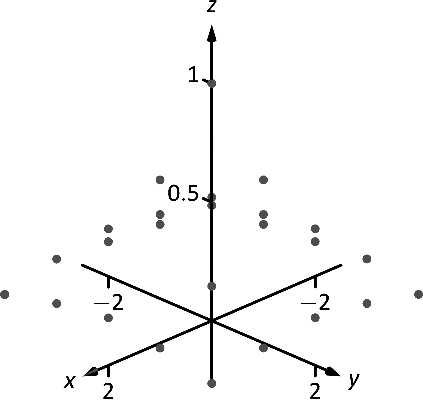
\includegraphics[width=0.43\textwidth]{fig_multi_var_1a}}
\qquad
\subfigure[\label{fig_multi_var_1b}]{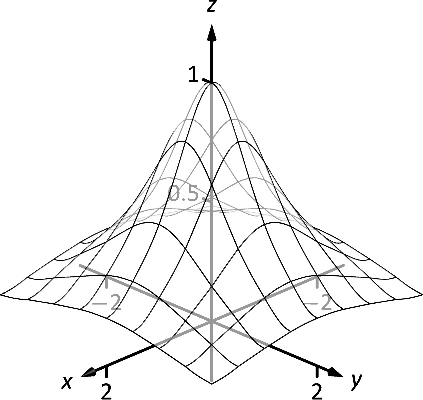
\includegraphics[width=0.43\textwidth]{fig_multi_var_1b} }
\caption{Graphing a function of two variables. }
\end{figure}


While technology is readily available to help us graph functions of two variables, there is still a paper--and--pencil approach that is useful to understand and master as it, combined with high--quality graphics, gives one great insight into the behaviour of a function. This technique is known as sketching \textbf{level curves} (\textit{ niveaukromme}).\index{level curve}\index[aut]{niveaukromme}\index[aut]{contourlijn}

It may be surprising to find that the problem of representing a three dimensional surface on paper is familiar to most people.\index{contour lines} Topographical maps, like the one of Dinant shown in Figure \ref{fig_multi_var_3}, represent the surface of Earth by indicating points with the same elevation with \textbf{contour lines} (\textit{countourlijn}). The elevations marked are equally spaced; in this example, each thin line indicates an elevation change in 10m increments and each thick line indicates a change of 50m. When lines are drawn close together, elevation changes rapidly. When lines are far apart,  elevation changes more gradually as one has to walk farther to rise 10m.

\begin{figure}
	\begin{center}
			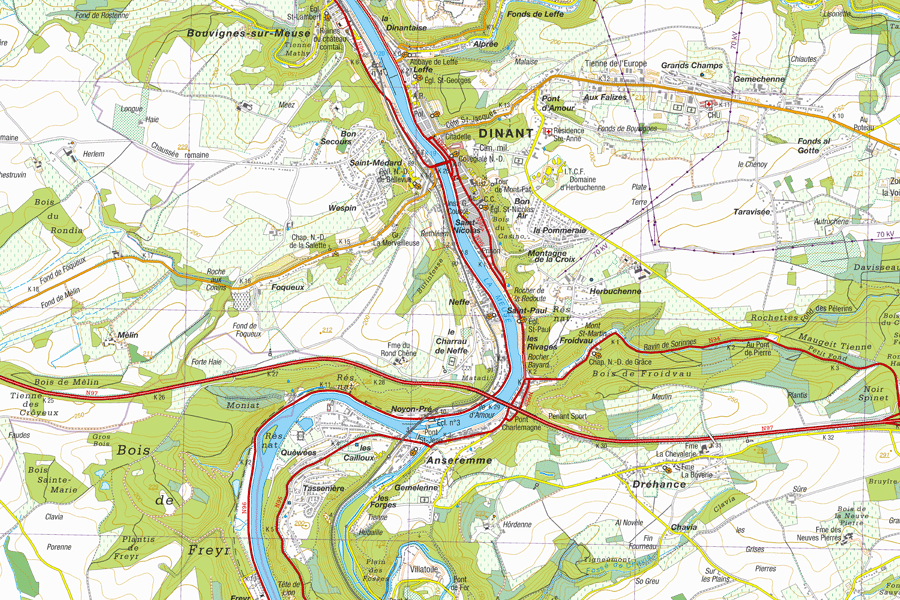
\includegraphics[width=0.5\textwidth]{fig_multi_var_3}
	\caption{The topographical map of Dinant displays elevation by drawing contour lines, along which the elevation is constant.}
	\label{fig_multi_var_3}
	\end{center}
\end{figure}

Given a function $z=f(x,y)$, we can draw a topographical map of $f$ by drawing \textbf{level curves} (or, contour lines). A level curve at $z=c$ is a curve in the $xy$-plane such that for all points $(x,y)$ on the curve, $f(x,y) = c$.  When drawing level curves, it is important that the $c$-values are spaced equally apart as that gives the best insight to how quickly the elevation is changing. 

\begin{example}\label{ex_levelcurves2}
Let $$\ds f(x,y) = \frac{x+y}{x^2+y^2+1}.$$ 
Find level curves.

\xhrulefill{gray}{2.5pt}Solution \xhrulefill{gray}{2.5pt}

We begin by setting $f(x,y)=c$ for an arbitrary $c$ and seeing if algebraic manipulation of the equation reveals anything significant.
\begin{equation*}
\frac{x+y}{x^2+y^2+1}  = c \qquad\qquad \Leftrightarrow \qquad\qquad x^2-\dfrac{1}{c}x+y^2-\dfrac{1}{c}y = -1.
\end{equation*}
We recognize this as a circle, though the centre and radius are not yet clear. By completing the square, we obtain:
$$
\left(x-\frac{1}{2c}\right)^2+\left(y-\frac1{2c}\right)^2=\frac{1}{2c^2}-1$$
a circle centred at $\big(1/(2c),1/(2c)\big)$ with radius $\sqrt{1/(2c^2)-1}$, where $|c|<1/\sqrt{2}$. The level curves for $c=\pm 0.2,\ \pm 0.4$ and $\pm0.6$ are sketched in Figure \ref{fig_multi_var_4a}. To help illustrate  elevation, we use dashed lines where $c<0$. There is one special level curve, when $c=0$. The level curve in this situation is $x+y=0$, the line $y=-x$.

In Figure \ref{fig_multi_var_4b} we see a graph of the surface. Note how the $y$-axis is pointing away from the viewer to more closely resemble the orientation of the level curves in Figure~\ref{fig_multi_var_4a}. Seeing the level curves helps us understand the graph. For instance, the graph does not make it clear that one can walk along the line $y=-x$ without elevation change, though the level curve does.

\begin{figure}[H]
\centering
%\raisebox{0.5cm}{
\subfigure[\label{fig_multi_var_4a}]{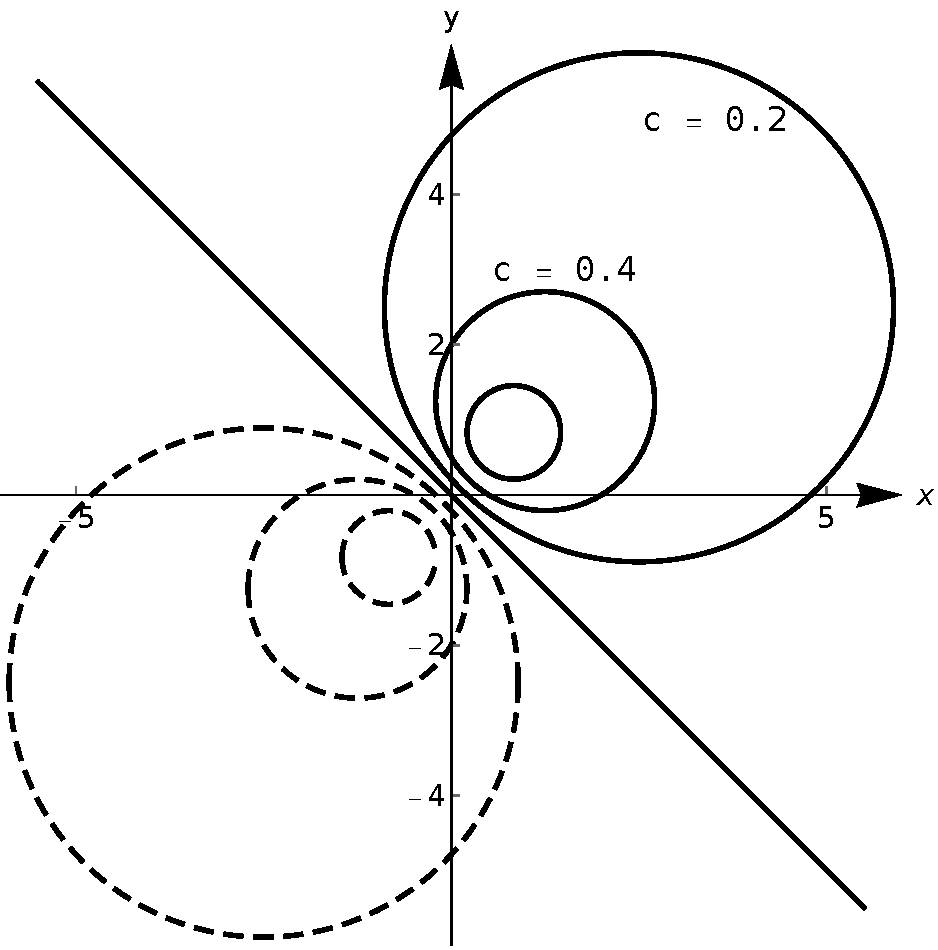
\includegraphics[width=0.43\textwidth]{fig_multi_var_4a}}
\qquad
\subfigure[\label{fig_multi_var_4b}]{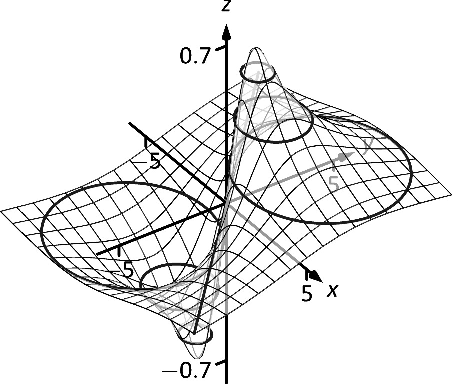
\includegraphics[width=0.43\textwidth]{fig_multi_var_4b} }
\caption{Graphing the level curves in Example \ref{ex_levelcurves2}. }
\end{figure}
\end{example}

%%%%% Vertalen naar het ENG

The contour lines are established as intersection between the surface defined by $z=f(x,y)$ with the horizontal plane $z=c$. However, there are two more special types of planes with which we can intersect the surface and which improve our understanding of functions of two variables, namely $x=x_0$ and $y=y_0$. These are planes perpendicular to the $x$- or $y$-axis. The  curves of intersection that we thus obtain  are  nothing more than the graphs of the so-called partial functions to $y$ or $x$.

\begin{definition}[Partial functions]
Let $f:\mathbb{R}^2\to\mathbb{R}$ be a function of two variables, then 
\begin{itemize}
    \item the partial function of $f$ with regard to $x$, or the first partial function is given by:
    $$
    f_1:\mathbb{R}\to\mathbb{R}: x\to z=f_1(x)=f(x,y_0)\,,
    $$
    with $y_0$ constant;
    \item the partial function of $f$ with regard to $y$,  or the second partial function is given by:
    $$
    f_2:\mathbb{R}\to\mathbb{R}: x\to z=f_2(y)=f(x_0,y)\,,
    $$
    with $x_0$ constant.    
\end{itemize}
\end{definition}

%%%%%

\ifcalculus
\subsection{Functions of three variables}

We extend our study of multivariable functions to functions of three variables. One can make a function of as many variables as one likes; we limit our study to three variables.

\begin{definition}[Function of three variables]\label{def:multi3}
Let $D$ be a subset of $\mathbb{R}^3$. A \textbf{function $f$ of three variables} (\textit{functie van drie veranderlijken}) is a rule that assigns each triple $(x,y,z)$ in $D$ a value $w=f(x,y,z)$ in $\mathbb{R}$. $D$ is the domain of $f$; the set of all outputs of $f$ is the range.
\index{multivariable function}\index{domain}\index{range}\index{function!of three variables}\index[aut]{domain}\index[aut]{bereik}
\end{definition}

It is very difficult to produce a meaningful graph of a function of three variables. A function of one variable is a curve drawn in 2 dimensions; a function of two variables is a surface drawn in 3 dimensions; a function of three variables is a \textbf{hypersurface} (\textit{hyperoppervlak}) drawn in 4 dimensions.\index{hypersurface}\index[aut]{hyperoppervlak}
\fi

\ifanalysis
\pagebreak
\subsection{Functions of $n$ variables}

We extend our study of multivariable functions to functions of $n$ variables. 

\begin{definition}[Function of $n$ variables]\label{def:multi3}
Let $D$ be a subset of $\mathbb{R}^n$. A \textbf{function $f$ of $n$ variables} is a rule that assigns each $\mathbf{x}=(x_1,x_2,\ldots,x_n)$ in $D$ a value $w=f(x_1,x_2,\ldots,x_n)=f(\mathbf{x})$ in $\mathbb{R}$. $D$ is the domain of $f$; the set of all outputs of $f$ is the range.
\index{multivariable function}\index{domain}\index{range}\index{function!of $n$ variables}\index[aut]{domain}\index[aut]{bereik}
\end{definition}

Note that in this definition, we are using the notation $\mathbf{x}$ to abbreviate the $n$-tuple $(x_1,x_2,\ldots,x_n)$. 
It is very difficult to produce a meaningful graph of a function of three variables. A function of one variable is a curve drawn in 2 dimensions; a function of two variables is a surface drawn in 3 dimensions; a function of $n$ variables is a \textbf{hypersurface} (\textit{hyperoppervlak}) drawn in $n+1$ dimensions.\index{hypersurface}\index[aut]{hyperoppervlak}

\fi


There are a few techniques one can employ to try to picture a graph of three variables. One is an analogue of level curves: \textbf{level surfaces} (\textit{ niveau-oppervlak}). Given $w=f(x,y,z)$, the level surface at $w=c$ is the surface in space formed by all points $(x,y,z)$ where $f(x,y,z)=c$. \index{level surface}\index[aut]{niveau-oppervlak}\index[aut]{contourlijn}

\begin{example}\label{ex_multi4}
If a point source $S$ is radiating energy, the intensity $I$ at a given point $P$ in space is inversely proportional to the square of the distance between $S$ and $P$. That is, when $S=(0,0,0)$,  
$$\ds I(x,y,z) = \frac{k}{x^2+y^2+z^2}$$
 for some constant $k$.

Let $k=1$; find the level surfaces of $I$.

\xhrulefill{gray}{2.5pt}Solution \xhrulefill{gray}{2.5pt}

We can  answer this question using common sense. If energy is emanating from the origin, its intensity will be the same at all points equidistant from the origin. That is, at any point on the surface of a sphere centred at the origin, the intensity should be the same. Therefore, the level surfaces are spheres.
We now find this mathematically. The level surface at $I=c$ for $c>0$ is defined by 
\begin{align*}
c &= \frac{1}{x^2+y^2+z^2}.
\intertext{A small amount of algebra reveals}
x^2+y^2+z^2 &= \frac1c.
\end{align*}
Given an intensity $c$, the level surface $I=c$ is a sphere of radius $1/\sqrt{c}$, centred at the origin. Table \ref{tab_multi_var_1} gives the radii of the spheres for given $c$-values. Normally one would use equally spaced $c$-values, but these values have been chosen purposefully. At a distance of 0.25 from the point source, the intensity is 16; to move to a point of half that intensity, one just moves out 0.1 to 0.35 -- not much at all. To again halve the intensity, one moves 0.15, a little more than before.

\begin{table}[H]
\caption{A table of $c$-values and corresponding radius $r$ of the spheres of constant value in Example \ref{ex_multi4}.}
\label{tab_multi_var_1}
\renewcommand{\arraystretch}{1.5}
\begin{tabular}{c|ccccccccc}
$c$ &16.&8.&4.&2.&1.&0.5&0.25&0.125&0.0625\\ \hline
$r$&0.25&0.35&0.5&0.71&1&1.41&2&2.83&4\\ 
\end{tabular}
\renewcommand{\arraystretch}{1}
\end{table}

Note how each time the intensity is halved, the distance required to move away grows. We conclude that the closer one is to the source, the more rapidly the intensity changes.
\end{example}

\ifanalysis
Finally, we note that the notion of partial functions can be extended to functions of $n$ variables. Let $f:\mathbb{R}^n\to\mathbb{R}$ a function of $n$ variables, than we call:
    $$
    f_i:\mathbb{R}\to\mathbb{R}: x_i\to z=f_i(x_i)=f(c_1,c_2,\ldots,c_{i-1},x_i,c_{i+1},\ldots,c_n)\,,
    $$
    with $c_j$ constant for $i=1,\ldots,n\, (j\neq i)$, the $i$-th partial function of $f$.
\fi

\section{Limits and continuity of multivariable functions}\label{sec:multi_limit}
This section investigates what it means for multivariable functions to be continuous.
\subsection{Introductory concepts and definitions}





\ifcalculus
We begin with a series of definitions. We are used to open  and closed intervals. We need analogous definitions for open and closed sets in the $xy$-plane.

\begin{definition}[Points and sets]\label{def:open}
An \textbf{open disk} (\textit{open schijf}) $B$ in $\mathbb{R}^2$ centred at $(x_0,y_0)$ with radius $r$ is the set of all points $(x,y)$ such that $\ds\sqrt{(x-x_0)^2+(y-y_0)^2} < r$. \\

Let $S$ be a set of points in $\mathbb{R}^2$. A point $P$ in $\mathbb{R}^2$ is a \textbf{boundary point} (\textit{randpunt}) of $S$  if all open disks centred at $P$ contain both points in $S$ and points not in $S$.\\

A point $P$ in $S$ is an \textbf{interior point} (\textit{inwendig punt}) of $S$ if there is an open disk centred at $P$ that contains only points in $S$. \\

A set $S$ is \textbf{open} (\textit{open}) if every point in $S$ is an interior point.\\

A set $S$ is \textbf{closed} (\textit{gesloten}) if it contains all of its boundary points.\\

A set $S$ is \textbf{bounded} (\textit{begrensd}) if there is an $M>0$ such that the open disk, centred at the origin with radius $M$, contains $S$. A set that is not bounded is unbounded.\\

A set $S$ is \textbf{convex} (\textit{convex}) if, given any two points, it contains the whole line segment that joins. A set that is not convex is called non-convex.


\index{open}\index{closed}\index{open disk}\index{closed disk}\index{boundary point}\index{interior point}\index{bounded set}\index{unbounded set}\index{convex set}
\index[aut]{inwendig punt}\index[aut]{open bol}\index[aut]{gesloten bol}\index[aut]{open verzameling}\index[aut]{gesloten verzameling}\index[aut]{begrensde verzameling}\index[aut]{onbegrensde verzameling}\index[aut]{randpunt}\index[aut]{convexe verzameling}
\end{definition}
\fi


\ifanalysis
We begin with a series of definitions. We are used to open  and closed intervals. We need analogous definitions for open and closed sets in the $n$-dimensional space.

\begin{definition}[Points and sets]\label{def:open}
An \textbf{open ball} (\textit{open bal}) $B$ in $\mathbb{R}^n$ centred at $\mathbf{x}_0$ with radius $r$ is the set of all points $\mathbf{x}$ such that $d(\mathbf{x},\mathbf{x}_0) < r$. \\[0.2cm]
Let $S$ be a set of points in $\mathbb{R}^n$. A point $P$ in $\mathbb{R}^n$ is a \textbf{boundary point} (\textit{randpunt}) of $S$  if all open disks centred at $P$ contain both points in $S$ and points not in $S$.\\[0.2cm]
A point $P$ in $S$ is an \textbf{interior point} (\textit{inwendig punt}) of $S$ if there is an open disk centred at $P$ that contains only points in $S$. \\[0.2cm]
A set $S$ is \textbf{open} (\textit{open}) if every point in $S$ is an interior point.\\[0.2cm]
A set $S$ is \textbf{closed} (\textit{gesloten}) if it contains all of its boundary points.\\[0.2cm]
A set $S$ is \textbf{bounded} (\textit{begrensd}) if there is an $M>0$ such that the open disk, centred at the origin with radius $M$, contains $S$. A set that is not bounded is unbounded.\\
A set $S$ is \textbf{convex} (\textit{convex}) if, given any two points, it contains the whole line segment that joins. A set that is not convex is called non-convex.


\index{open}\index{closed}\index{open disk}\index{closed disk}\index{boundary point}\index{interior point}\index{bounded set}\index{unbounded set}\index{convex set}
\index[aut]{inwendig punt}\index[aut]{open bol}\index[aut]{gesloten bol}\index[aut]{open verzameling}\index[aut]{gesloten verzameling}\index[aut]{begrensde verzameling}\index[aut]{onbegrensde verzameling}\index[aut]{randpunt}\index[aut]{convexe verzameling}
\end{definition}
\fi



Figure \ref{fig_multi_var_5} shows several sets in the $xy$-plane. In each set, point $P_1$ lies on the boundary of the set as all open disks centred there contain both points in, and not in, the set. In contrast, point $P_2$ is an interior point for there is an open disk centred there that lies entirely within the set. The set depicted in Figure \ref{fig_multi_var_5a} is a closed set as it contains all of its boundary points. The set in Figure~\ref{fig_multi_var_5b} is open, for all of its points are interior points (or, equivalently, it does not contain any of its boundary points). The set in Figure~\ref{fig_multi_var_5c} is neither open nor closed as it contains  some of its boundary points. Finally, it should be clear that all sets shown in Figure \ref{fig_multi_var_5} are non-convex because we can easily find pairs of points that can only be connected by a straight line that is not completely contained in the considered sets. 

\begin{figure}
\centering
%\raisebox{0.5cm}{
\subfigure[\label{fig_multi_var_5a}]{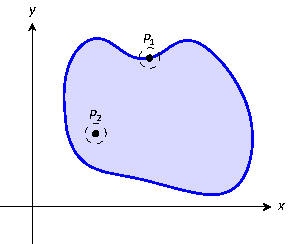
\includegraphics[width=0.33\textwidth]{fig_multi_var_5a}}
\qquad
\subfigure[\label{fig_multi_var_5b}]{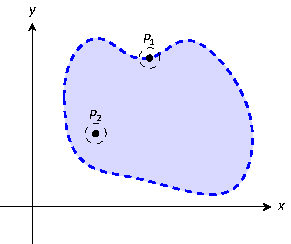
\includegraphics[width=0.33\textwidth]{fig_multi_var_5b} }
\qquad
\subfigure[\label{fig_multi_var_5c}]{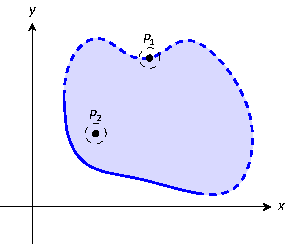
\includegraphics[width=0.33\textwidth]{fig_multi_var_5c} }
\caption{Illustrating open and closed sets in the $xy$-plane.}
\label{fig_multi_var_5}
\end{figure}

\ifanalysis\pagebreak\fi
\begin{example}\label{ex_multilimit1}
Determine if the domain of the functions 
\begin{multicols}{2}
\begin{enumerate}
\item $f(x,y)=\sqrt{1-\dfrac{x^2}9-\dfrac{y^2}4}$
\item  $g(x,y) = \dfrac{1}{x-y}$
\end{enumerate}
\end{multicols}
 is open, closed, or neither, and if it is bounded.

\xhrulefill{gray}{2.5pt}Solution \xhrulefill{gray}{2.5pt}

\begin{enumerate}
\item The domain of this function was found in Example \ref{ex_multi2} to be 
$$D = \bigg\{(x,y)\,\, \bigg| \,\, \frac{x^2}9+\frac{y^2}4\leq 1\bigg\},$$ the region bounded by the ellipse $\frac{x^2}{9}+\frac{y^2}{4}=1$. Since the region includes the boundary, the set contains all of its boundary points and hence is closed. The region is bounded as a disk of radius 4, centred at the origin, contains $D$.
\item As we cannot divide by 0, we find the domain to be $D = \big\{(x,y) \,\, \big|\,\, x-y\neq 0\big\}$. In other words, the domain is the set of all points $(x,y)$ not on the line $y=x$. 
The domain is sketched in Figure \ref{fig_multi_var_6}. Note how we can draw an open disk around any point in the domain that lies entirely inside the domain, and also note how the only boundary points of the domain are the points on the line $y=x$. We conclude the domain is an open set. The set is unbounded.
\end{enumerate}
\begin{figure}[H]
	\begin{center}
			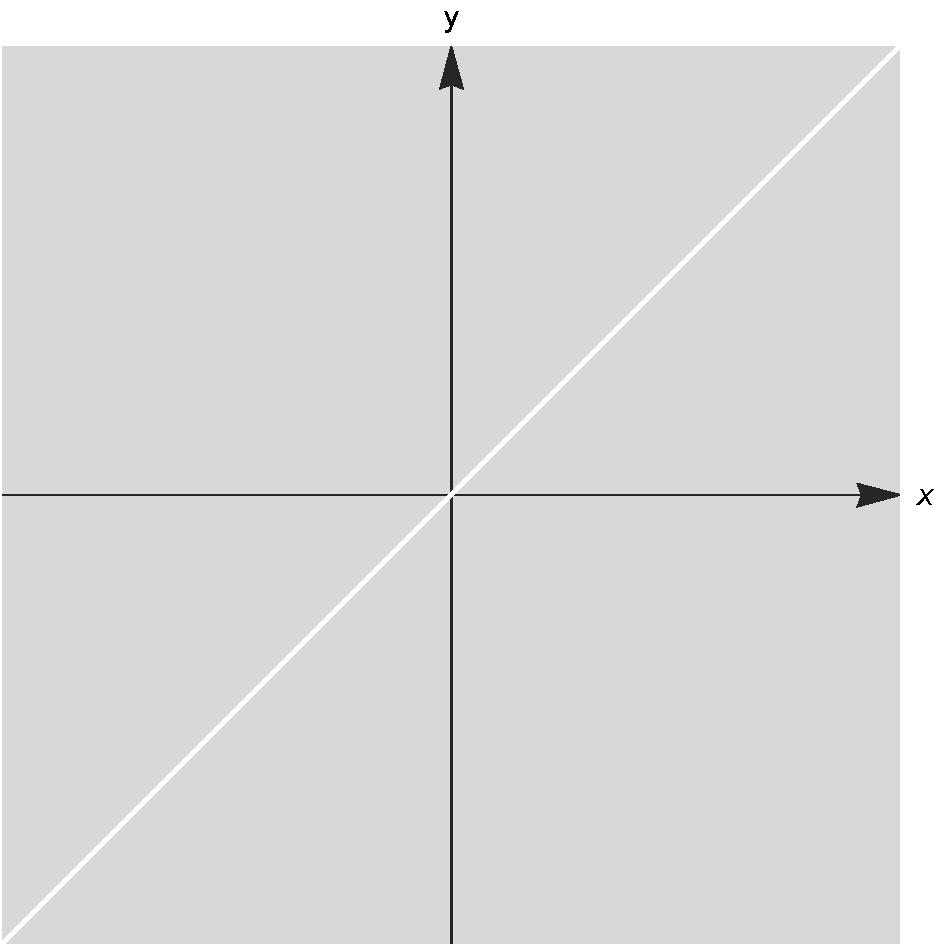
\includegraphics[width=0.5\textwidth]{fig_multi_var_6}
	\caption{Sketching the domain of the function in Example \ref{ex_multilimit1}.2.}
	\label{fig_multi_var_6}
	\end{center}
\end{figure}
\end{example}

\subsection{Limits}
\ifcalculus
We will say that 


\begin{center}
$\ds \lim_{(x,y)\to (x_0,y_0)} f(x,y) = L$ \end{center}
means if the point $(x,y)$ is really close to the point $(x_0,y_0)$, then $f(x,y)$ is really close to $L$. The formal definition is given below.



%\setboxwidth{40pt}

\begin{definition}[Limit of a function of two variables]\label{def:multilimita}
Let $S$ be a set containing $P=(x_0,y_0)$ where every open disk centred at $P$ contains points in $S$ other than $P$, i.e.\ $P$ is a limit point, let $f$ be a function of two variables defined on $S$, except possibly at $P$, and let $L$ be a real number. 
%Let $f(x,y)$ be a function of two variables and let $(x_0,y_0)$ be a point in the domain of $f$. 
The \textbf{limit of $f(x,y)$ as $(x,y)$ approaches $(x_0,y_0)$} is $L$, denoted $$\ds \lim_{(x,y)\to (x_0,y_0)} f(x,y) = L,$$
means that given any $\varepsilon>0$, there exists $\delta>0$ such that for all  $(x,y)$ in $S$, where $(x,y)\neq (x_0,y_0)$, if $(x,y)$ is in the open disk centred at $(x_0,y_0)$ with radius $\delta$, then $|f(x,y) - L|<\varepsilon.$
\index{limit!of multivariable function}\index{multivariable function!limit}\index[aut]{limiet}
\end{definition}
\fi


\ifanalysis
We will say that 


\begin{center}
$\ds \lim_{(x,y)\to (x_0,y_0)} f(x,y) = L$ \end{center}
means if the point $(x,y)$ is really close to the point $(x_0,y_0)$, then $f(x,y)$ is really close to $L$. The formal definition for a function of $n$ variables is given below.



%\setboxwidth{40pt}

\begin{definition}[Limit of a function of $n$ variables]\label{def:multilimita}
Let $S$ be a set containing $P=\mathbf{x}_0$ where every open disk centred at $P$ contains points in $S$ other than $P$, i.e.\ $P$ is a limit point, let $f$ be a function of two variables defined on $S$, except possibly at $P$, and let $L$ be a real number. 
%Let $f(x,y)$ be a function of two variables and let $(x_0,y_0)$ be a point in the domain of $f$. 
The \textbf{limit of $f(\mathbf{x})$ as $\mathbf{x}$ approaches $\mathbf{x}_0$} is $L$, denoted $$\ds \lim_{\mathbf{x}\to \mathbf{x}_0} f(\mathbf{x}) = L,$$
means that given any $\varepsilon>0$, there exists $\delta>0$ such that for all  $\mathbf{x}$ in $S$, where $\mathbf{x}\neq \mathbf{x}_0$, if $\mathbf{x}$ is in the open ball centred at $\mathbf{x}_0$ with radius $\delta$, then $|f(\mathbf{x}) - L|<\varepsilon.$
\index{limit!of multivariable function}\index{multivariable function!limit}\index[aut]{limiet}
\end{definition}
\fi


Note that we now define limits over a set $S$ in the plane (where $S$ does not have to be open). As planar sets can be far more complicated than intervals, our definition adds the restriction ``$\ldots$ where every open disk centred at $P$ contains points in $S$ other than $P$.'' This means that $P$ should be a so-called \textbf{limit point} (\textit{ophopingspunt}) of the set $S$. This in contrast to a so-called \textbf{isolated point} (\textit{g\"eisoleerd punt}) $Q$ of $S$ for which there exists a neighbourhood of $Q$ which does not contain any other points of $S$.\index{limit point}\index[aut]{ophopingspunt}\index[aut]{limietpunt}\index{isolated point}\index[aut]{ge\"eisoleerd punt}


The concept behind Definition~\ref{def:multilimita} is sketched in Figure \ref{fig_multi_var_7}. Given $\varepsilon>0$, find $\delta>0$ such that if $(x,y)$ is any point in the open disk centred at $(x_0,y_0)$ in the $xy$-plane with radius $\delta$, then $f(x,y)$ should be within $\varepsilon$ of $L$. 

\begin{figure}[H]
	\begin{center}
			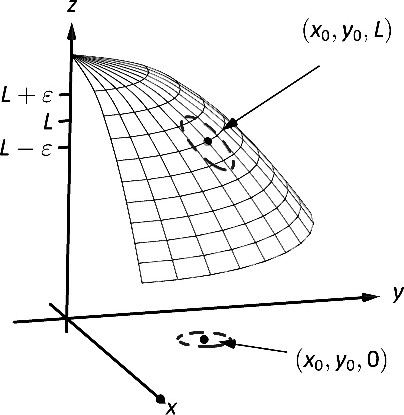
\includegraphics[width=0.5\textwidth]{fig_multi_var_7}
	\caption{Illustrating the definition of a limit of a function of two variables.}
	\label{fig_multi_var_7}
	\end{center}
\end{figure}

\ifcalculus
Computing limits using this definition is rather cumbersome. The following properties allow us to evaluate limits much more easily. For that purpose, let $b$, $x_0$, $y_0$, $L$ and $K$ be real numbers,  let $n$ be a positive integer, and let $f$ and $g$ be functions with the following limits:
$$\lim_{(x,y)\to (x_0,y_0)}f(x,y) = L \quad \text{\ and\ } \lim_{(x,y)\to (x_0,y_0)} g(x,y) = K.$$
The following limits hold.

\begin{itemize}
\item \textbf{Constants:} $$\displaystyle \lim_{(x,y)\to (x_0,y_0)} b = b$$
\item	\textbf{Identity }	$$\displaystyle \lim_{(x,y)\to (x_0,y_0)} x = x_0;\qquad \displaystyle \lim_{(x,y)\to (x_0,y_0)} y = y_0$$
\item	\textbf{Sums/Differences:} $$\displaystyle \lim_{(x,y)\to (x_0,y_0)}\big(f(x,y)\pm g(x,y)\big) = L\pm K$$
\item	\textbf{Scalar Multiples:}	$$\displaystyle \lim_{(x,y)\to (x_0,y_0)} b\cdot f(x,y) = bL$$
\item	\textbf{Products:}	$$\displaystyle \lim_{(x,y)\to (x_0,y_0)} f(x,y)\cdot g(x,y) = LK$$
\item	\textbf{Quotients:} $$\displaystyle \lim_{(x,y)\to (x_0,y_0)} f(x,y)/g(x,y) = L/K,\qquad (K\neq 0)$$
\item	\textbf{Powers:} 	$$\displaystyle \lim_{(x,y)\to (x_0,y_0)} \big[f(x,y)\big]^n = L^n$$
%\item	\parbox{80pt}{Roots:}		\parbox[t]{185pt}{$\displaystyle \lim_{(x,y)\to (x_0,y_0)} \sqrt[n]{f(x,y)} = \sqrt[n]{L}$}% \qquad \small (if $n$ is even then $L$ must be greater than 0; when $n$ is odd, it is true for all $L$.)}

\end{itemize}
\fi



\ifanalysis
Computing limits using this definition is rather cumbersome. The following properties allow us to evaluate limits much more easily. For that purpose, let $\mathbf{x}=(x_1,x_2,\ldots,x_n)$, let $\mathbf{x}_0$ have real components $(x_{0})_i$ and let $b$, $L$ and $K$ be real numbers,  let $n$ be a positive integer, and let $f$ and $g$ be functions with the following limits:
$$\lim_{\mathbf{x}\to \mathbf{x}_0}f(\mathbf{x}) = L \quad \text{\ and\ } \lim_{\mathbf{x}\to \mathbf{x}_0} g(\mathbf{x}) = K.$$
The following limits hold.

\begin{itemize}
\item \textbf{Constants:} $$\displaystyle \lim_{\mathbf{x}\to \mathbf{x}_0} b = b$$
\item	\textbf{Identity }	$$\displaystyle \lim_{\mathbf{x}\to \mathbf{x}_0} x_i = (x_{0})_i$$
\item	\textbf{Sums/Differences:} $$\displaystyle \lim_{\mathbf{x}\to \mathbf{x}_0}\big(f(\mathbf{x})\pm g(\mathbf{x})\big) = L\pm K$$
\item	\textbf{Scalar Multiples:}	$$\displaystyle \lim_{\mathbf{x}\to \mathbf{x}_0} b\cdot f(\mathbf{x}) = bL$$
\item	\textbf{Products:}	$$\displaystyle \lim_{\mathbf{x}\to \mathbf{x}_0} f(\mathbf{x})\cdot g(\mathbf{x}) = LK$$
\item	\textbf{Quotients:} $$\displaystyle \lim_{\mathbf{x}\to \mathbf{x}_0} \dfrac{f(\mathbf{x})}{g(\mathbf{x}} = \dfrac{L}{K},\qquad (K\neq 0)$$
\item	\textbf{Powers:} 	$$\displaystyle \lim_{\mathbf{x}\to \mathbf{x}_0} \big[f(\mathbf{x})\big]^n = L^n$$
%\item	\parbox{80pt}{Roots:}		\parbox[t]{185pt}{$\displaystyle \lim_{(x,y)\to (x_0,y_0)} \sqrt[n]{f(x,y)} = \sqrt[n]{L}$}% \qquad \small (if $n$ is even then $L$ must be greater than 0; when $n$ is odd, it is true for all $L$.)}

\end{itemize}
\fi


These properties, combined with the ones we introduced in Chapter~\ref{chap_limits}, allow us to evaluate many limits. For instance, we can easily evaluate
$$
	\lim_{(x,y)\to (1,\pi)} \left(\frac yx + \cos(xy)\right)  = \frac\pi{1}+\cos (\pi) = \pi -1.
$$
\ifmathematica
This limit may as well be evaluated in Mathematica with a nested application of the command \lstinline{Limit}.\index{\lstinline{Limit}}\index[aut]{\lstinline{Limit}}
	\begin{mdframed}[default,backgroundcolor=gray!40,roundcorner=8pt]
\begin{mmaCell}[morefunctionlocal={x,y}]{Input}
  Limit[Limit[y/x + Cos[x*y], x -> 1], y -> Pi]
\end{mmaCell}

\begin{mmaCell}{Output}
  -1+\(\pi\)
\end{mmaCell}
\end{mdframed}
\fi

\ifpython
This limit may as well be evaluated in Mathematica with a nested application of the command \lstinline{limit}.
\begin{pyin}
from sympy import symbols, limit, pi, cos
x, y = symbols('x y')
limit(limit(y/x + cos(x*y), x, 1), y, pi)
\end{pyin}
\begin{pyout}
-1+\pi
\end{pyout}
\fi


When dealing with functions of a single variable we also considered one--sided limits and stated
$$\lim_{x\to c}f(x) = L$$
if, and only if
$$
\lim_{x\underset{>}{\rightarrow}c}f(x) =L \quad \mbox{and}\quad \lim_{x\underset{<}{\rightarrow}c}f(x) =L.
$$
That is, the limit is $L$ if and only if $f(x)$ approaches $L$ when $x$ approaches $c$ from either direction, the left or the right.

In the plane, there are infinitely many directions from which $(x,y)$ might approach $(x_0,y_0)$. In fact, we do not have to restrict ourselves to approaching $(x_0,y_0)$ from a particular direction, but rather we can approach that point along a path that is not a straight line. It is possible to arrive at different limiting values by approaching $(x_0,y_0)$ along different paths. If this happens, we say that $\ds \lim_{(x,y)\to(x_0,y_0) } f(x,y)$ does not exist. This is analogous to the left and right hand limits of single variable functions not being equal.

Our theorems tell us that we can evaluate most limits quite simply, without worrying about  paths. When indeterminate forms arise, the limit may or may not exist. If it does exist, it can be difficult to prove this as we need to show the same limiting value is obtained regardless of the path chosen. The case where the limit does not exist is often easier to deal with, for we can often pick two paths along which the limit is different.

\begin{example}\label{ex_multilimit4}
\begin{enumerate}
	\item Show $$\ds \lim_{(x,y)\to (0,0)} \frac{3xy}{x^2+y^2}$$ does not exist by finding the limits along the lines $y=mx$.
	\item	Show $$\ds \lim_{(x,y)\to (0,0)} \frac{\sin(xy)}{x+y}$$ does not exist by finding the limit along the path $y=-\sin (x)$. 	
\end{enumerate}

\pagebreak
\xhrulefill{gray}{2.5pt}Solution \xhrulefill{gray}{2.5pt}

\begin{enumerate}
	\item Evaluating this limit along the lines $y=mx$ means replace all $y$'s with $mx$ and evaluating the resulting limit:
	\begin{align*}
	\lim_{(x,mx)\to (0,0)} \frac{3x(mx)}{x^2+(mx)^2} &=\lim_{x\to 0} \frac{3mx^2}{x^2(m^2+1)}\\[0.2cm]
				&= \lim_{x\to 0} \frac{3m}{m^2+1}\\[0.2cm]
				&= \frac{3m}{m^2+1}.
	\end{align*}
	While the limit exists for each choice of $m$, we get a different limit for each choice of $m$. That is, along different lines we get differing limiting values, meaning the limit does not exist.
	
	\item We are to show that $\ds \lim_{(x,y)\to (0,0)} f(x,y)$ does not exist by finding the limit along the path $y=-\sin (x)$. First, however, consider the limits found along the lines $y=mx$ as done above.
	\begin{align*}
	\lim_{(x,mx)\to (0,0)} \frac{\sin\big(x(mx)\big)}{x+mx} &= \lim_{x\to 0} \frac{\sin (mx^2)}{x(m+1)} \\[0.2cm]
	&= \lim_{x\to 0} \frac{\sin(mx^2)}{x}\cdot\frac1{m+1}.
	\end{align*}
	By applying L'H\^opital's rule, we can show this limit is 0 except when $m=-1$, that is, along the line $y=-x$. This line is not in the domain of $f$, so we have found the following fact: along every line $y=mx$ in the domain of $f$, $$\ds \lim_{(x,y)\to(0,0)} f(x,y)=0.$$ %Along this line, $f(x,y)$ is not defined, so it stands to reason that a limit along this line does not exist.
	
	Now consider the limit along the path $y=-\sin (x)$:
	\begin{align*}
	\lim_{(x,-\sin (x))\to (0,0)} \frac{\sin\big(-x\sin x\big)}{x-\sin (x)} &= \lim_{x\to0} \frac{\sin\big(-x\sin x\big)}{x-\sin (x)}\,.
	\end{align*}
	Now apply L'H\^opital's rule twice:
	\begin{align*}
	 \quad &= \lim_{x\to 0}\frac{\cos\big(-x\sin (x)\big)(-\sin (x)-x\cos (x))}{1-\cos (x)} \quad \left(= \dfrac{0}{0}\right)\\[0.2cm]
	&= \lim_{x\to 0}\frac{-\sin\big(-x\sin (x)\big)(-\sin (x)-x\cos (x))^2+\cos\big(-x\sin (x)\big)(-2\cos (x)+x\sin (x))}{\sin (x)}\\[0.2cm]
	&= \text{$\dfrac{-2}{0}$}.  
	\end{align*}
	It follows that the limit does not exist.
Step back and consider what we have just discovered. Along any line $y=mx$ in the domain of the $f(x,y)$, the limit is 0. However, along the path $y=-\sin (x)$, which lies in the domain of  $f(x,y)$ for all $x\neq 0$, the limit does not exist. Since the limit is not the same along every path to $(0,0)$, we say that the studied limit does not exist.
\end{enumerate}
\end{example}

\ifanalysis
\begin{example}\label{ex_multilimit5}

Let 
$$\ds f(x,y) = \frac{5x^2y^2}{x^2+y^2}.$$
Find $\ds\lim_{(x,y)\to (0,0)}  f(x,y) .$

\xhrulefill{gray}{2.5pt}Solution \xhrulefill{gray}{2.5pt}

It is relatively easy to show that along any line $y=mx$, the limit is 0. This is not enough to prove that the limit exists, as demonstrated in the previous example, but it tells us that if the limit does exist then it must be 0.

To prove the limit is 0, we apply Definition \ref{def:multilimita}. Let $\varepsilon >0$ be given. We want to find $\delta >0$ such that if $\sqrt{(x-0)^2+(y-0)^2} <\delta$, then $|f(x,y)-0| <\varepsilon$.

Set $\delta < \sqrt{\varepsilon/5}$. Note that $\ds \left|\frac{5y^2}{x^2+y^2}\right| <5$ for all $(x,y)\neq (0,0)$, and that if $\sqrt{x^2+y^2} <\delta$, then $x^2<\delta^2$.

Let $\sqrt{(x-0)^2+(y-0)^2} = \sqrt{x^2+y^2}<\delta$. Consider $|f(x,y)-0|$:
\begin{align*}
|f(x,y)-0| &= \left|\frac{5x^2y^2}{x^2+y^2}-0\right| \\
				&= \left|x^2\cdot\frac{5y^2}{x^2+y^2}\right|\\
				&< \delta^2\cdot 5 \\
				&< \frac{\varepsilon}{5}\cdot 5 \\
				&= \varepsilon.
\end{align*}
Thus if $\sqrt{(x-0)^2+(y-0)^2}<\delta$ then $|f(x,y)-0|<\varepsilon$, which is what we wanted to show. Thus $$\ds \lim_{(x,y)\to(0,0)} \frac{5x^2y^2}{x^2+y^2} = 0\,.$$

\end{example}
\fi

\subsection{Continuity}
Definition \ref{def:continuous} defines what it means for a function of one variable to be continuous. In brief, it meant that the graph of the function did not have breaks, holes, jumps, etc. We define continuity for functions of two variables in a similar way as we did for functions of one variable.

\ifcalculus
\begin{definition}[Continuity]\label{def:multi_continuous}
Let a function $f(x,y)$ be defined on a set $S$ containing the point $(x_0,y_0)$. 

\begin{enumerate}
	\item $f$ is continuous at $(x_0,y_0)$ if $\ds\lim_{(x,y)\to(x_0,y_0)} f(x,y) = f(x_0,y_0)$.
	\index{continuous function}\index{multivariable function!continuity}\index[aut]{functie ! continue}
	\item	$f$ is \textbf{continuous on $S$} (\textit{continu over}) if $f$ is continuous at all points in $S$. If $f$ is continuous at all points in $\mathbb{R}^2$, we say that $f$ is continuous everywhere.
\end{enumerate}
\end{definition}
\fi

\ifanalysis
\begin{definition}[Continuity]\label{def:multi_continuous}
Let a function $f(\mathbf{x})$ be defined on a set $S$ containing the point $\mathbf{x}_0$. 

\begin{enumerate}
	\item $f$ is continuous at $\mathbf{x}_0$ if $\ds\lim_{\mathbf{x}\to\mathbf{x}_0} f(\mathbf{x}) = f(\mathbf{x}_0)$.
	\index{continuous function}\index{multivariable function!continuity}\index[aut]{functie ! continue}
	\item	$f$ is \textbf{continuous on $S$} (\textit{continu over}) if $f$ is continuous at all points in $S$. If $f$ is continuous at all points in $\mathbb{R}^n$, we say that $f$ is continuous everywhere.
\end{enumerate}
\end{definition}
\fi

\begin{example}\label{ex_multicont1}
Let $$\ds f(x,y) = \left\{ \begin{array}{ll} \dfrac{\cos (y)\sin(x)}{x}, & \quad x\neq 0 \\
																						\cos(y), & \quad x=0.
													\end{array} \right.$$ Is $f$ continuous at $(0,0)$? Is $f$ continuous everywhere?

\xhrulefill{gray}{2.5pt}Solution \xhrulefill{gray}{2.5pt}

To determine if $f$ is continuous at $(0,0)$, we need to compare $\ds\lim_{(x,y)\to (0,0)} f(x,y)$ to $f(0,0)$. 
Applying the definition of $f$, we see that $f(0,0) = \cos(0) = 1$. 

We now consider the limit $\ds \lim_{(x,y)\to (0,0)} f(x,y)$. Substituting $0$ for $x$ and $y$ in $f(x,y)$ returns the indeterminate form ``0/0'', so we need to do more work to evaluate this limit.

Consider two related limits: 
$$\ds \lim_{(x,y)\to (0,0)} \cos(y)\qquad\text{and}\qquad \ds \lim_{(x,y)\to(0,0)} \frac{\sin(x)}x.$$ The first limit does not contain $x$, and since $\cos(y)$ is continuous, $$\ds \lim_{(x,y)\to (0,0)} \cos(y) =\lim_{y\to 0} \cos(y) = \cos(0) = 1.$$

The second limit does not contain $y$. By Theorem \ref{thm:special_limits} we can say
$$\lim_{(x,y)\to (0,0)} \frac{\sin(x)}{x} = \lim_{x\to 0} \frac{\sin(x)}{x} = 1.$$
Finally, following the properties of limits we can combine these two limits as follows:
\allowdisplaybreaks
\begin{align*}
\lim_{(x,y)\to (0,0)} \frac{\cos(y)\sin(x)}{x} &= \lim_{(x,y)\to (0,0)} \left(\cos(y)\left(\frac{\sin(x)}{x}\right)\right) \\ 
 & =\left(\lim_{(x,y)\to (0,0)} \cos(y)\right)\left(\lim_{(x,y)\to (0,0)} \frac{\sin(x)}{x}\right) \\
  & = (1)(1)=1.
\end{align*}

We have found that $$\ds \lim_{(x,y)\to (0,0)} \frac{\cos(y)\sin(x)}{x} = f(0,0),$$ so $f$ is continuous at $(0,0)$.

A similar analysis shows that $f$ is continuous at all points in $\mathbb{R}^2$. As long as $x\neq0$, we can evaluate the limit directly; when $x=0$, a similar analysis shows that the limit is $\cos(y)$. Thus we can say that $f$ is continuous everywhere. A graph of $f$ is given in Figure \ref{fig_multi_var_8}. Notice how it has no breaks, jumps, etc.

\begin{figure}[H]
	\begin{center}
			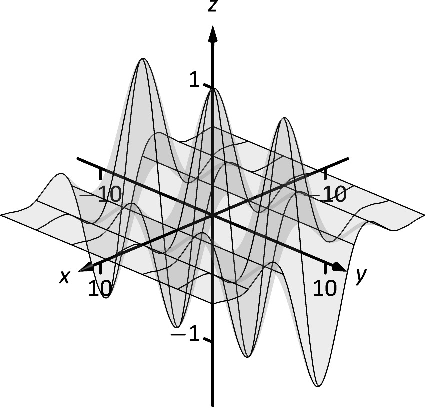
\includegraphics[width=0.5\textwidth]{fig_multi_var_8}
	\caption{A graph of $f(x,y)$ in Example \ref{ex_multicont1}.}
	\label{fig_multi_var_8}
	\end{center}
\end{figure}


\end{example}

Of course, as with functions of one variable, we may combine continuous functions to create other continuous functions. More specifically, let $f$ and $g$ be continuous on a set $S$, let $c$ be a real number, and let $n$ be a positive integer. Then, the following functions are continuous on $S$.
		\begin{itemize}
		\item		\textbf{Sums/Differences:}	$f\pm g$
		\item		\textbf{Constant multiples:}	$c\cdot f$
		\item		\textbf{Products:}	$f\cdot g$
		\item		\textbf{Quotients:}	$f/g$ \qquad  (if $g\neq 0$ on $S$)
		\item		\textbf{Powers:}	$f\,^n$
\end{itemize}
For roots of a continuous function, we have that $\sqrt[n]{f}$ is continuous provided that $f\geq 0$ on $S$ if $n$ is even, whereas, if $n$ is odd, this is true for all values of $f$ on $S$. For what concerns function compositions, we let $f$ be continuous on $S$, where the range of $f$ on $S$ is $J$, and let $g$ be a single variable function that is continuous on $J$. Then $g\circ f$, i.e., $g(f(x,y))$, is continuous on $S$.

\ifcalculus
\subsection{Functions of three variables}

The definitions and theorems given in this section can be extended in a natural way to definitions and theorems about functions of three variables. We cover the key concepts here; some terms from Definitions \ref{def:open} and \ref{def:multi_continuous} are not redefined but their analogous meanings should be clear to the reader.


\begin{definition}[Open balls, limit and continuity]\label{def:multi3defs}
\begin{enumerate}
\item An \textbf{open ball} (\textit{open bal}) in $\mathbb{R}^3$ centred at $(x_0,y_0,z_0)$ with radius $r$ is the set of all points $(x,y,z)$ such that $\sqrt{(x-x_0)^2+(y-y_0)^2+(z-z_0)^2} = r$.
\index{multivariable function!limit}\index{limit!of multivariable function}\index{multivariable function!continuity}\index{open ball}\index[aut]{open bal}\index[aut]{functie ! limiet}

\item Let $D$ be a set in $\mathbb{R}^3$ containing $(x_0,y_0,z_0)$ where every open ball centred at $(x_0,y_0,z_0)$ contains points of $D$ other than $(x_0,y_0,z_0)$, and let $f(x,y,z)$ be a function of three variables defined on $D$, except possibly at  $(x_0,y_0,z_0)$. The \textbf{limit of $f(x,y,z)$ as $(x,y,z)$ approaches $(x_0,y_0,z_0)$} is $L$, denoted 
$$\lim_{(x,y,z)\to (x_0,y_0,z_0)} f(x,y,z) = L,$$
means that given any $\varepsilon >0$, there is a $\delta >0$ such that for all  $(x,y,z)$ in $D$, $(x,y,z)\neq(x_0,y_0,z_0)$, if $(x,y,z)$ is in the open ball centred at $(x_0,y_0,z_0)$ with radius $\delta$, then $|f(x,y,z) - L|< \varepsilon$.\\

\item Let $f(x,y,z)$ be defined on a set $D$ containing $(x_0,y_0,z_0)$. $f$ is \textbf{continuous at $(x_0,y_0,z_0)$} if $$\ds \lim_{(x,y,z)\to (x_0,y_0,z_0)} f(x,y,z) = f(x_0,y_0,z_0)$$; if $f$ is continuous at all points in $D$, we say $f$ is continuous on $D$.
\end{enumerate}
\end{definition}

\fi

%\ifanalysis
%\subsection{Functions of $n$ variables}
%
%The definitions and theorems given in this section can be extended in a natural way to definitions and theorems about functions of $n$ variables. We cover the key concepts here; some terms from Definitions \ref{def:open} and \ref{def:multi_continuous} are not redefined but their analogous meanings should be clear to the reader.
%

%\begin{definition}[Open balls, limit and continuity]\label{def:multi3defs}
%
%\begin{enumerate}
%\item An open ball in $\mathbb{R}^n$ centred at $\mathbf{c}$ with radius $r$ is the set of all points $\mathbf{x}$ such that $d(\mathbf{c},\mathbf{x}) = r$.
%\index{multivariable function!limit}\index{limit!of multivariable function}\index{multivariable function!continuity}\index{open ball}\index[aut]{open bal}\index[aut]{functie ! limiet}

%\item Let $D$ be a set in $\mathbb{R}^n$ containing the limit point $\mathbf{c}$, and let $f(\mathbf{x})$ be a function of $n$ variables defined on $D$, except possibly at  $\mathbf{c}$. The limit of $f(\mathbf{x})$ as $\mathbf{x}$ approaches $\mathbf{c}$ is $L$, denoted 
%$$\lim_{\mathbf{x}\to \mathbf{c}} f(\mathbf{x}) = L,$$
%means that given any $\varepsilon >0$, there is a $\delta >0$ such that for all  $\mathbf{x}$ in $D$, $\mathbf{x}\neq\mathbf{c}$, if $\mathbf{x}$ is in the open ball centred at $\mathbf{c}$ with radius $\delta$, then $|f(\mathbf{x}) - L|< \varepsilon$.\\

%\item Let $f(\mathbf{x})$ be defined on a set $D$ containing $(\mathbf{c})$. $f$ is continuous at $\mathbf{c}$ if $\ds \lim_{\mathbf{x}\to \mathbf{c}} f(\mathbf{x}) = f(\mathbf{c})$; if $f$ is continuous at all points in $D$, we say $f$ is continuous on $D$.
%\end{enumerate}
%
%\end{definition}


%Theorem \ref{thm:multi_continuous_prop} also applies to function of three or more variables, allowing us to say that the function $$\ds f(x,y,z) = \frac{e^{x^2+y}\sqrt{y^2+z^2+3}}{\sin (xyz)+5}$$ is continuous everywhere.


%\fi


\ifanalysis

Having introduced the notion of continuity for functions of $n$ variables, the multivariable counterpart of the indermediate value theorem follows intuitively. 

\begin{theorem}[Intermediate value theorem for functions of $n$ variables]\label{thm:IVTmulti}
Let $f$ be a continuous function on $D$ and, without loss of generality, let $f(\mathbf{a}) < f(\mathbf{b})$. Then for every value $u$, where $f(\mathbf{a}) < u < f(\mathbf{b})$, there is at least one interior point $\mathbf{c}$ in $D$ such that $f(\mathbf{c}) = u$. \index{Intermediate value theorem}\index[aut]{Tussenwaardestelling}
\end{theorem}



\fi

When considering single variable functions, we studied limits, then continuity, then the derivative. In our current study of multivariable functions, we have studied limits and continuity. In the next section we study derivation, which takes on a slight twist as we are in a multivarible context.

\section{Partial derivatives}\label{sec:partial_derivatives}
\subsection{First partial derivatives}

	\checkoddpage
\marginpar{\ifoddpage\hspace*{-1.5cm}\else\hspace*{0.25cm}\fi
\includegraphics[width=0.075\textwidth]{youtube}\\
\ifoddpage\hspace*{-1.75cm}\else\hspace*{0.1cm}\fi
\qrcode[height=1.75cm]{https://youtu.be/dfvnCHqzK54}
%\includegraphics[width=0.1\textwidth]{partial}
}

Let $y$ be a function of $x$. We have studied in great detail the derivative of $y$ with respect to $x$, that is, which measures the rate at which $y$ changes with respect to $x$. Consider now $z=f(x,y)$. It makes sense to want to know how $z$ changes with respect to $x$ and/or $y$. This section begins our investigation into these rates of change.

Consider the function $z=f(x,y) = x^2+2y^2$, as graphed in Figure \ref{fig_multi_var_9a}. By fixing $y=2$, we focus our attention to all points on the surface where the $y$-value is 2, shown in Figures~\ref{fig_multi_var_9a} and \ref{fig_multi_var_9b}. These points form a curve in space: $z = f(x,2) = x^2+8$ which is a function of just one variable. We can take the derivative of $z$ with respect to $x$ along this curve and find equations of tangent lines, etc. 


\begin{figure}[h]
\centering
%\raisebox{0.5cm}{
\subfigure[\label{fig_multi_var_9a}]{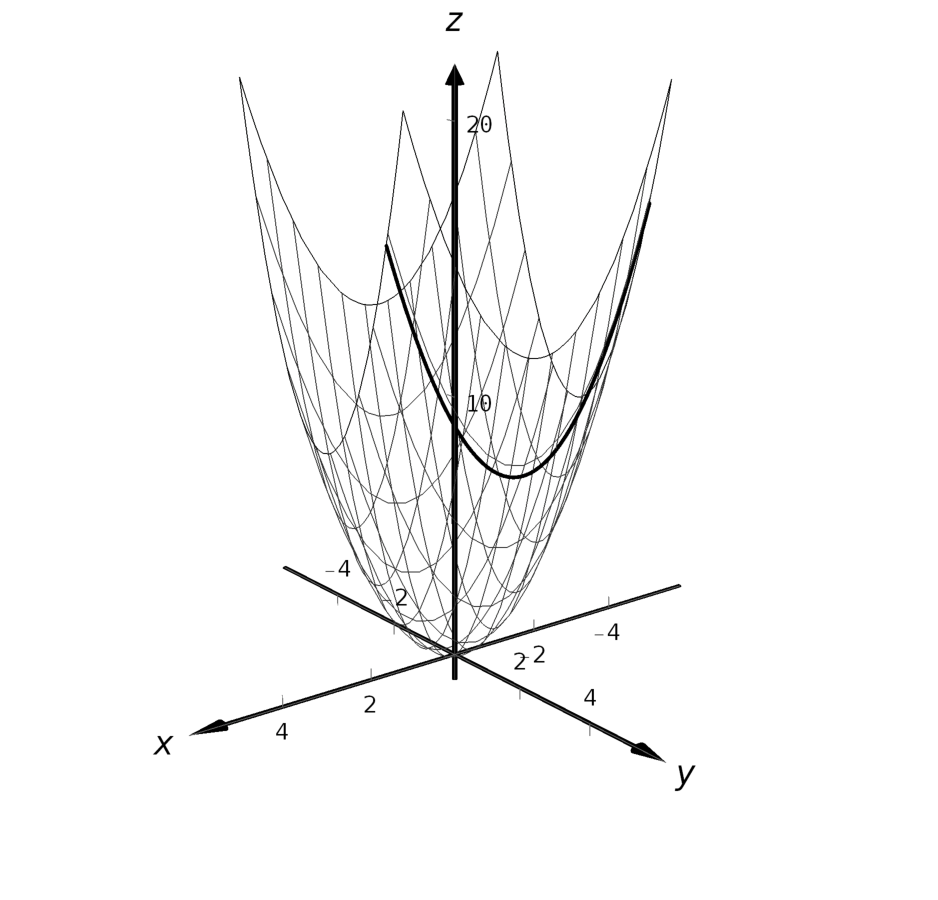
\includegraphics[width=0.43\textwidth]{fig_multi_var_9a}}
\qquad
\subfigure[\label{fig_multi_var_9b}]{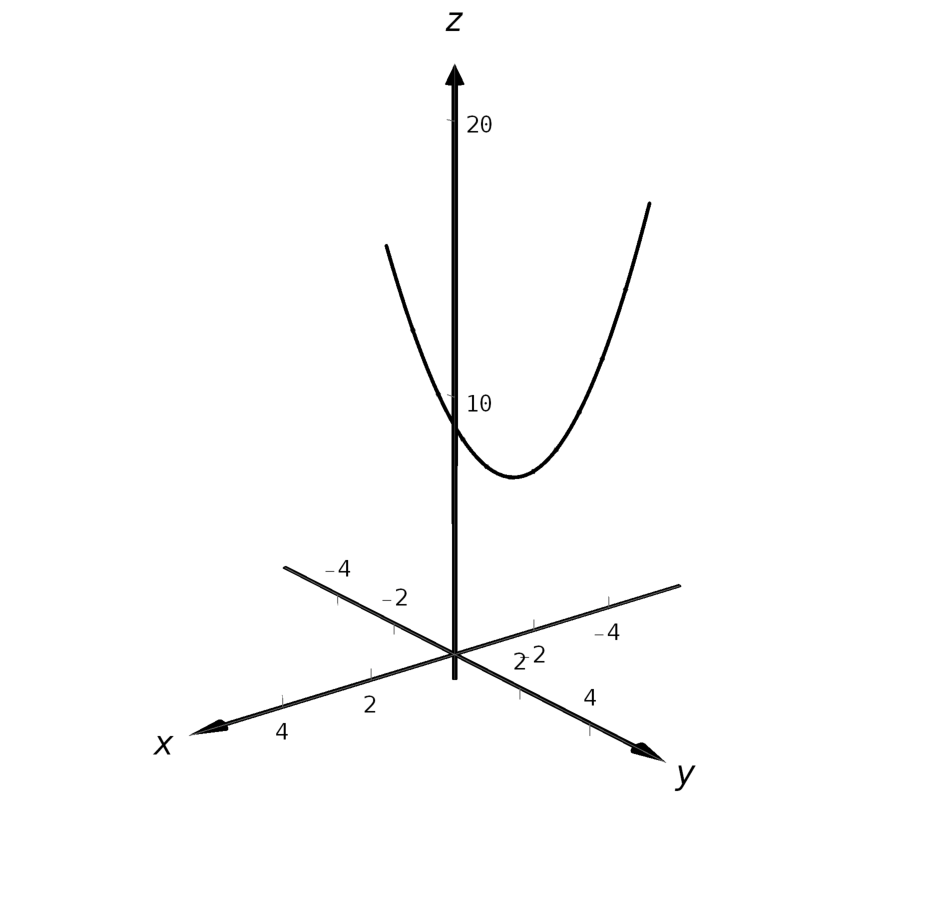
\includegraphics[width=0.43\textwidth]{fig_multi_var_9b} }
\caption{By fixing $y=2$, the surface $f(x,y) = x^2+2y^2$ is a curve in space.}
\end{figure}

The key notion to extract from this example is: by treating $y$ as  constant (it does not vary) we can consider how $z$ changes with respect to $x$. In a similar fashion, we can hold $x$ constant and consider how $z$ changes with respect to $y$. This is the underlying principle of \textbf{partial derivatives} (\textit{parti\"ele afgeleide}). We state the formal, limit--based definition first, then show how to compute these partial derivatives without directly taking limits.

\ifcalculus\pagebreak\fi
\begin{definition}[Partial derivative]\label{def:partial_derivative}
Let $z=f(x,y)$ be a continuous function on a set $S$ in $\mathbb{R}^2$.
\begin{enumerate}
	\item The \textbf{partial derivative of $f$ with respect to $x$} is:
	$$f_x(x,y) = \lim_{h\to 0} \frac{f(x+h,y) - f(x,y)}h.$$
	%Alternate notations for $\frac{\partial z}{\partial x}$ include: $\ds\frac{\partial}{\partial x}f(x,y),\ f_x(x,y),\ \text{and}\ z_x.$
	\item The \textbf{partial derivative of $f$ with respect to $y$} is:
	$$f_y(x,y) = \lim_{h\to 0} \frac{f(x,y+h) - f(x,y)}h.$$
	
	%\item		If $f_x$ and $f_y$ are continuous on $S$, then $f$ is \textbf{differentiable} on $S$.\footnote{This definition of differentiability is mathematically ``weak'' but easy to understand; see Section \ref{sec:total_differential} for a stronger definition that is less intuitive.}
	\end{enumerate}
	\index{partial derivative}\index{derivative!partial}\index[aut]{afgeleide ! partieel}\index[aut]{parti\"ele afgeleide}
\end{definition}

Alternate notations for $f_x(x,y)$ include: $$\frac{\partial}{\partial x}f(x,y),\ \ \frac{\pf}{\px},\ \ \frac{\pz}{\px},\ \ \text{and}\ z_x,$$ with similar notations for $f_y(x,y).$ For ease of notation, $f_x(x,y)$ is often abbreviated as $f_x$.

\ifanalysis
\begin{example}\label{ex_partial1}

Let $f(x,y) = x^2y + 2x+y^3$. Find $f_x(x,y)$ using the limit definition.

\xhrulefill{gray}{2.5pt}Solution \xhrulefill{gray}{2.5pt}

Using Definition \ref{def:partial_derivative}, we have:
\begin{align*}
f_x(x,y) &= \lim_{h\to 0} \frac{f(x+h,y) - f(x,y)}{h} \\
				&= \lim_{h\to 0} \frac{(x+h)^2y+2(x+h)+y^3 - (x^2y+2x+y^3)}{h}\\
				&= \lim_{h\to 0} \frac{x^2y+2xhy+h^2y+2x+2h+y^3-(x^2y+2x+y^3)}{h}\\
				&= \lim_{h\to 0} \frac{2xhy+h^2y+2h}{h}\\
				&=\lim_{h\to 0} \left(2xy+hy+2 \right)\\
				&= 2xy+2.
\end{align*}
We have found $f_x(x,y) = 2xy+2$.

\end{example}
\fi

Using limits to compute partial derivatives is not necessary, as we can rely on our previous knowledge of derivatives to compute partial derivatives easily. When computing $f_x(x,y)$, we hold $y$ fixed -- it does not vary. Therefore we can compute the derivative with respect to $x$ by treating $y$ as a constant or coefficient. 

\ifcalculus\pagebreak\fi
\begin{example}\label{ex_partial2}
Find $f_x(x,y)$ and $f_y(x,y)$ for each of the following functions.
\begin{multicols}{2}
\begin{enumerate}
	\item	$f(x,y) = \cos(xy^2)+\sin(x)$
	\item	$f(x,y) = e^{x^2y^3}\sqrt{x^2+1}$
\end{enumerate} 
\end{multicols}

\xhrulefill{gray}{2.5pt}Solution \xhrulefill{gray}{2.5pt}

\begin{enumerate}	
	\item Begin with $f_x(x,y)$. We need to apply the chain rule with the cosine term; $y^2$ is the coefficient of the $x$-term inside the cosine function.
	$$f_x(x,y) = -\sin(xy^2)(y^2)+\cos(x) = -y^2\sin(xy^2)+\cos(x).$$
	To find $f_y(x,y)$, note that $x$ is the coefficient of the $y^2$-term inside of the cosine term; also note that since $x$ is fixed, $\sin(x)$ is also fixed, and we treat it as a constant.
	$$f_y(x,y) = -\sin(xy^2)(2xy) = -2xy\sin(xy^2).$$
\ifmathematica
	We may check our answer for what concerns $f_x$ in Mathematica as follows:  \index{\lstinline{D}}\index[aut]{\lstinline{D}}
	\begin{mdframed}[default,backgroundcolor=gray!40,roundcorner=8pt]
\begin{mmaCell}[morefunctionlocal={x}]{Input}
  D[Cos[x*y^2] + Sin[x], x]
\end{mmaCell}

\begin{mmaCell}{Output}
  Cos[x]-\mmaSup{y}{2} Sin[x \mmaSup{y}{2}]
\end{mmaCell}
\end{mdframed}
And likewise for what concerns $f_y$:
	\begin{mdframed}[default,backgroundcolor=gray!40,roundcorner=8pt]
\begin{mmaCell}[morefunctionlocal={x}]{Input}
  D[Cos[x*y^2] + Sin[x], y]
\end{mmaCell}

\begin{mmaCell}{Output}
  -2 x y Sin[x \mmaSup{y}{2}]
\end{mmaCell}
\end{mdframed}
\fi

\ifpython
We may check our answer for what concerns $f_x$ in Python as follows:
\begin{pyin}
from sympy import symbols, cos, sin, diff
x, y = symbols('x y')
diff(cos(x*y**2)+sin(x), x)
\end{pyin}
\begin{pyout}
-y^2 \sin(xy^2) + \cos(x)
\end{pyout}
And likewise for what concerns $f_y$:
\begin{pyin}
from sympy import symbols, cos, sin, diff
x, y = symbols('x y')
diff(cos(x*y**2)+sin(x), y)
\end{pyin}
\begin{pyout}
-2xy \sin(xy^2)
\end{pyout}
\fi
	\item		Beginning with $f_x(x,y)$, note how we need to apply the product rule. 
	\begin{align*}
	f_x(x,y) &= e^{x^2y^3}(2xy^3)\sqrt{x^2+1} + e^{x^2y^3}\frac12\big(x^2+1\big)^{-1/2}(2x) \\[0.2cm]
					&= 2xy^3e^{x^2y^3}\sqrt{x^2+1}+\frac{xe^{x^2y^3}}{\sqrt{x^2+1}}.
	\end{align*}
	Note that when finding $f_y(x,y)$ we do not have to apply the product rule; since $\sqrt{x^2+1}$ does not contain $y$, we treat it as fixed and hence becomes a coefficient of the $e^{x^2y^3}$-term.
	$$f_y(x,y) = e^{x^2y^3}(3x^2y^2)\sqrt{x^2+1} = 3x^2y^2e^{x^2y^3}\sqrt{x^2+1}.$$
\end{enumerate}
\end{example}

We have shown how to compute a partial derivative, but it may still not be clear what a partial derivative means. Given $z=f(x,y)$, $f_x(x,y)$ measures the rate at which $z$ changes as only $x$ varies: $y$ is held constant. 

Imagine standing in a rolling meadow, then beginning to walk due east. Depending on your location, you might walk up, sharply down, or perhaps not change elevation at all. This is similar to measuring $z_x$: you are moving only east (in the $x$-direction) and not north/south at all. Going back to your original location, imagine now walking due north (in the $y$-direction). Perhaps walking due north does not change your elevation at all. This is analogous to $z_y=0$: $z$ does not change with respect to $y$. We can see that $z_x$ and $z_y$ do not have to be the same, or even similar, as it is easy to imagine circumstances where walking east means you walk downhill, though walking north makes you walk uphill. 

\subsection{Second partial derivatives}
Let $z=f(x,y)$. We have learned to find the partial derivatives $f_x(x,y)$ and $f_y(x,y)$, which are each functions of $x$ and $y$. Therefore we can take partial derivatives of them, each with respect to $x$ and $y$. We define these second partials along with the notation, give examples, then discuss their meaning.

\ifanalysis\pagebreak\fi
\begin{definition}[Second and mixed partial derivative]\label{def:second_partial}
Let $z=f(x,y)$ be continuous on a set $S$.
\begin{enumerate}
	\item The \textbf{second partial derivative of $f$ with respect to $x$ then $x$} (\textit{tweede parti\"ele afgeleide van $f$ naar $x$}) is $$\frac{\partial}{\partial x}\left(\frac{\partial f}{\px}\right) = \frac{\partial^2 f}{\px^2} = \big(\,f_x\,\big)_x = f_{xx}.$$

\item The \textbf{second partial derivative of $f$ with respect to $x$ then $y$ is} (\textit{tweede parti\"ele afgeleide van $f$ naar $x$ en $y$})  is $$\frac{\partial}{\partial y}\left(\frac{\partial f}{\px}\right) = \frac{\partial^2f}{\py\px} = \big(\,f_x\,\big)_y = f_{xy}.$$
\end{enumerate}
Similar definitions hold for $\ds \frac{\partial^2f}{\py^2} = f_{yy}$ and $\ds \frac{\partial^2f}{\px\py} = f_{yx}$. 
The second partial derivatives $f_{xy}$ and $f_{yx}$ are \textbf{mixed partial derivatives} (\textit{gemengde parti\"ele afgeleide}).
\index{partial derivative!mixed}\index{partial derivative!second derivative}\index{derivative!mixed partial}\index[aut]{parti\"ele afgeleide ! gemengd}\index[aut]{parti\"ele afgeleide ! tweede}
\end{definition}

The terms in Definition \ref{def:second_partial} all depend on limits, so each definition comes with the caveat where the limit exists.

\begin{example}\label{ex_partial6}
For each of the following functions, find all 6 first and second partial derivatives. That is, find 
$$f_x,\quad f_y,\quad f_{xx},\quad f_{yy},\quad f_{xy}\quad \text{and}\quad f_{yx}\,.$$
\begin{multicols}{2}
\begin{enumerate}
	\item	$\ds f(x,y) = \frac{x^3}{y^2}$
	\item	$f(x,y)=e^{x}\sin(x^2y)$
\end{enumerate}
\end{multicols}
\xhrulefill{gray}{2.5pt}Solution \xhrulefill{gray}{2.5pt}

In each, we give $f_x$ and $f_y$ immediately and then spend time deriving the second partial derivatives.

\begin{enumerate}	
	\item		$\ds f(x,y) = \frac{x^3}{y^2} = x^3y^{-2}$
\begin{multicols}{2}
	$\ds f_x(x,y) = \frac{3x^2}{y^2}$\\
	$\ds f_y(x,y) = -\frac{2x^3}{y^3}$\\
	$\ds f_{xx}(x,y) = \frac{\partial}{\px}\left(f_x\right) = \frac{\partial}{\px}\left(\frac{3x^2}{y^2}\right) = \frac{6x}{y^2}$\\		
$\ds f_{yy}(x,y) = \frac{\partial}{\py}\left(f_y\right) = \frac{\partial}{\py}\left(-\frac{2x^3}{y^3}\right) = \frac{6x^3}{y^4}$\\	
$\ds f_{xy}(x,y) = \frac{\partial}{\py}\left(f_x\right) = \frac{\partial}{\py}\left(\frac{3x^2}{y^2}\right) = -\frac{6x^2}{y^3}$\\
$\ds f_{yx}(x,y) = \frac{\partial}{\px}\left(f_y\right) = \frac{\partial}{\px}\left(-\frac{2x^3}{y^3}\right) = 
-\frac{6x^2}{y^3}$	
\end{multicols}
\item	$\ds f(x,y) = e^x\sin(x^2y)$

  Because the following partial derivatives get rather long, we omit the extra notation and just give the results. In several cases, multiple applications of the product and chain rules will be necessary, followed by some basic combination of like terms.


$\ds f_x(x,y) = e^x\sin(x^2y) + 2xye^x\cos(x^2y)$
	
	$\ds f_y(x,y) = x^2e^x\cos(x^2y)$
	
	$\ds f_{xx}(x,y) = e^x\sin(x^2y)+4xye^x\cos(x^2y)+2ye^x\cos(x^2y)-4x^2y^2e^x\sin(x^2y)$ 
	
	
		$\ds f_{yy}(x,y) =  -x^4e^x\sin(x^2y)$
		
		$\ds f_{xy}(x,y) = x^2e^x\cos(x^2y)+2xe^x\cos(x^2y)-2x^3ye^x\sin(x^2y)$
		
		$\ds f_{yx}(x,y) = x^2e^x\cos(x^2y)+2xe^x\cos(x^2y)-2x^3ye^x\sin(x^2y)$

\end{enumerate}
\end{example}

\ifmathematica
Higher-order partial derivatives can also be computed in Mathematica. For instance, given $ f(x,y) = x^3/y^2$ from Example~\ref{ex_partial6}, we can find $f_{xy}$ as follows:
	\begin{mdframed}[default,backgroundcolor=gray!40,roundcorner=8pt]
\begin{mmaCell}[morefunctionlocal={x,y}]{Input}
  D[x^3/y^2, x, y]
\end{mmaCell}

\begin{mmaCell}{Output}
  -\mmaFrac{6 \mmaSup{x}{2}}{\mmaSup{y}{3}}
\end{mmaCell}
\end{mdframed}
\fi

\ifpython
Higher-order partial derivatives can also be computed in Python. For instance, given $ f(x,y) = x^3/y^2$ from Example~\ref{ex_partial6}, we can find $f_{xy}$ as follows:
\begin{pyin}
from sympy import symbols, diff
x, y = symbols('x y')
diff(x**3/y**2, x, y)
\end{pyin}
\begin{pyout}
-\frac{6x^2}{y^3}
\end{pyout}
\fi

Notice how for each of the two functions in Example \ref{ex_partial6}, $f_{xy} = f_{yx}$. Due to the complexity of the examples, this likely is not a coincidence. The following theorem states that it is not. It is also known as \textbf{Schwarz's theorem}, \textbf{Clairaut's theorem}, or \textbf{Young's theorem}.

\begin{theorem}[Symmetry of second derivatives]\label{thm:mixed_partial}
Let $f$ be defined such that $f_{xy}$ and $f_{yx}$ are continuous on a set $S$. Then for each point $(x,y)$ in $S$, $f_{xy}(x,y) = f_{yx}(x,y)$.
\end{theorem}



Now that we know how to find second partials, we investigate what they tell us. 

Again we refer back to a function $y=f(x)$ of a single variable. The second derivative of $f$ is ``the derivative of the derivative,'' or ``the rate of change of the rate of change.'' The second derivative measures how much the derivative is changing. If $\fp'(x)<0$, then the derivative is getting smaller (so the graph of $f$ is concave down); if $\fp'(x)>0$, then the derivative is growing, making the graph of $f$ concave up. 

Now consider $z=f(x,y)$. Similar statements can be made about $f_{xx}$ and $f_{yy}$ as could be made about $\fp'(x)$ above. When taking derivatives with respect to $x$ twice, we measure how much $f_x$ changes with respect to $x$. If $f_{xx}(x,y)<0$, it means that as $x$ increases, $f_x$ decreases, and the graph of $f$ will be concave down in the $x$-direction. Using the analogy of standing in the rolling meadow used earlier in this section, $f_{xx}$ measures whether one's path is concave up/down when walking due east.
Similarly, $f_{yy}$ measures the concavity in the $y$-direction. If $f_{yy}(x,y)>0$, then $f_y$ is increasing with respect to $y$ and the graph of $f$ will be concave up in the $y$-direction. Appealing to the rolling meadow analogy again, $f_{yy}$ measures whether one's path is concave up/down when walking due north.

We now consider the mixed partials $f_{xy}$ and $f_{yx}$. The mixed partial $f_{xy}$ measures how much $f_x$ changes with respect to $y$. Once again using the rolling meadow analogy, $f_{x}$ measures the slope if one walks due east. Looking east, begin walking north (side--stepping). Is the path towards the east getting steeper? If so, $f_{xy}>0$. Is the path towards the east not changing in steepness? If so, then $f_{xy}=0$. A similar thing can be said about $f_{yx}$: consider the steepness of paths heading north while side--stepping to the east.

The following example examines these ideas with concrete numbers and graphs.

\begin{example}\label{ex_partial7}
Let $z=x^2-y^2+xy$. Evaluate the 6 first and second partial derivatives at $(-1/2,1/2)$ and interpret what each of these numbers mean.

\ifanalysis\pagebreak\fi
\xhrulefill{gray}{2.5pt}Solution \xhrulefill{gray}{2.5pt}

We find that:

$f_x(x,y) = 2x+y$,\quad  $f_y(x,y) = -2y+x$,\quad $f_{xx}(x,y) = 2$, \quad $f_{yy}(x,y) = -2$ and $f_{xy}(x,y) = f_{yx}(x,y) = 1$. Thus at $(-1/2,1/2)$ we have 
$$f_x\left(-\dfrac{1}{2},\dfrac{1}{2}\right) = -\dfrac{1}{2},\qquad f_y\left(-\dfrac{1}{2},\dfrac{1}{2}\right) = -\dfrac{3}{2}.$$
The slope of the tangent line at $(-1/2, 1/2, -1/4)$ in the direction of $x$ is $-1/2$: if one moves from that point parallel to the $x$-axis, the instantaneous rate of change will be $-1/2$. The slope of the tangent line
 at this point in the direction of $y$ is $-3/2$: if one moves from this point parallel to the $y$-axis, the instantaneous rate of change will be $-3/2$. These tangents lines are graphed in Figure \ref{fig_multi_var_10a} and \ref{fig_multi_var_10b}, together with the curve where $x=-1/2$ and $y=1/2$, respectively, where the tangent lines are drawn in a solid line. 

\begin{figure}[H]
\centering
%\raisebox{0.5cm}{
\subfigure[\label{fig_multi_var_10a}]{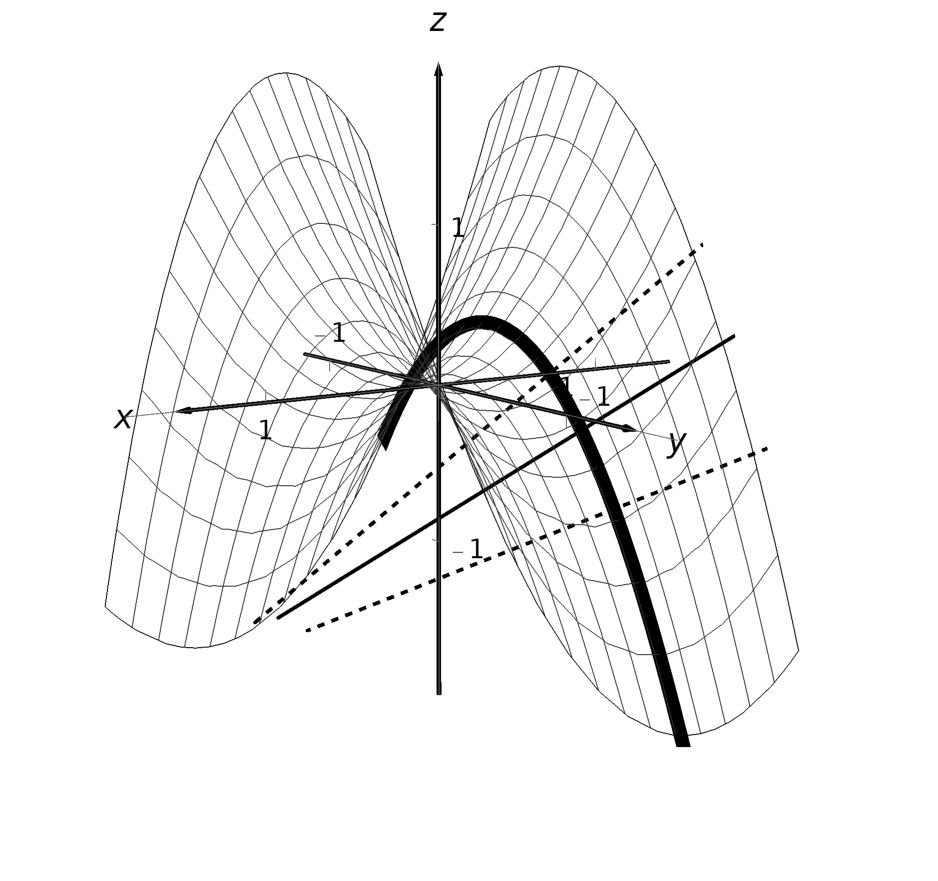
\includegraphics[width=0.43\textwidth]{fig_multi_var_10a}}
\qquad
\subfigure[\label{fig_multi_var_10b}]{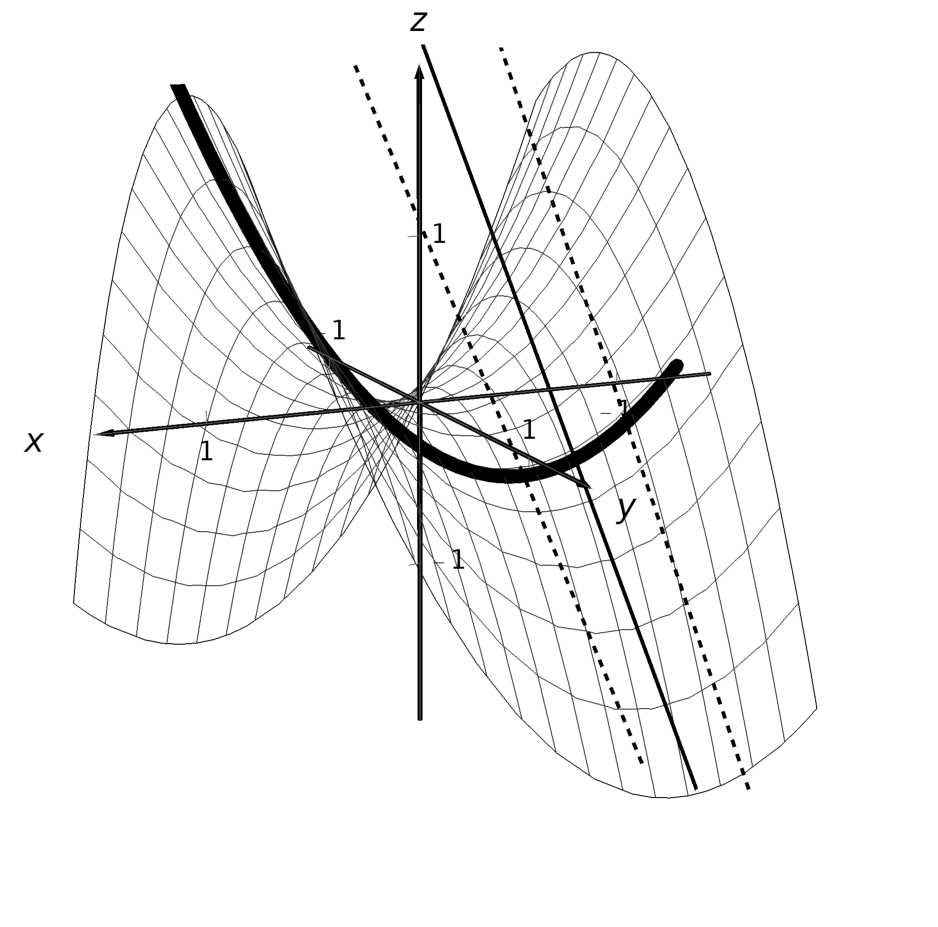
\includegraphics[width=0.43\textwidth]{fig_multi_var_10b} }
\caption{Understanding the second partial derivatives in Example \ref{ex_partial7}.}
\end{figure}


Now consider only Figure \ref{fig_multi_var_10a}. Three directed tangent lines are drawn (two are dashed), each in the direction of $x$; that is, each has a slope determined by $f_x$. Note how as $y$ increases, the slope of these lines get closer to $0$. Since the slopes are all negative, getting closer to 0 means the slopes are increasing. The slopes given by $f_x$ are increasing as $y$ increases, meaning $f_{xy}$ must be positive. 

Since $f_{xy}=f_{yx}$, we also expect $f_y$ to increase as $x$ increases. Consider Figure \ref{fig_multi_var_10b} where again three directed tangent lines are drawn, this time each in the direction of $y$ with slopes determined by $f_y$. As $x$ increases, the slopes become less steep (closer to 0). Since these are negative slopes, this means the slopes are increasing.

Thus far we have a visual understanding of $f_x$, $f_y$, and $f_{xy}=f_{yx}$. We now interpret $f_{xx}$ and $f_{yy}$. In Figure \ref{fig_multi_var_10a}, we see a curve drawn where $x$ is held constant at $x=-1/2$: only $y$ varies. This curve is clearly concave down, corresponding to the fact that $f_{yy}<0$. In Figure~\ref{fig_multi_var_10b}, we see a similar curve where $y$ is constant and only $x$ varies. This curve is concave up, corresponding to the fact that $f_{xx}>0$.
\end{example}

\subsection{Higher-order partial derivatives}
Essentially, we can continue taking partial derivatives of partial derivatives of partial derivatives of \ldots; we do not have to stop with second partial derivatives. These higher order partial derivatives do not have a tidy graphical interpretation; nevertheless they are not hard to compute and worthy of some practice. 
\index{partial derivative!high order}

We do not formally define each higher order derivative, but rather give just a few examples of the notation. For instance, 
$$f_{xyx}(x,y)  =\frac{\partial}{\px}\left(\frac{\partial}{\py}\left(\frac{\pf}{\px}\right)\right) \quad \text{ and }\quad
f_{xxz}(x,y)  =\frac{\partial}{\partial z}\left(\frac{\partial}{\px}\left(\frac{\pf}{\px}\right)\right)  .$$

\begin{example}\label{ex_partial9}
Let $$f(x,y) = x^2y^2+\sin(xy).$$
 Find $f_{xxy}$ and $f_{yxx}$. 

\xhrulefill{gray}{2.5pt}Solution \xhrulefill{gray}{2.5pt}

 To find $f_{xxy}$, we first find $f_x$, then $f_{xx}$, then $f_{xxy}$:
\begin{multicols}{2}
	$f_x = 2xy^2+y\cos(xy)$\\
	$f_{xx} = 2y^2-y^2\sin(xy)$\\
	$f_{xxy} = 4y-2y\sin(xy) - xy^2\cos(xy).$
	\end{multicols}
	To find $f_{yxx}$, we first find $f_y$, then $f_{yx}$, then $f_{yxx}$:
	\allowdisplaybreaks
	\begin{align*}
	f_y &= 2x^2y+x\cos(xy)\\
	f_{yx} &= 4xy + \cos(xy) - xy\sin(xy)\\
	f_{yxx} &= 4y-y\sin(xy) - \big(y\sin(xy) + xy^2\cos(xy)\big)\\ &= 4y-2y\sin(xy)-xy^2\cos(xy).
	\end{align*}
	
	Note how $f_{xxy} = f_{yxx}$.
	
\end{example}

In the previous example we saw that $f_{xxy} = f_{yxx}$; this is not a coincidence. While we do not state this as a formal theorem, as long as each partial derivative is continuous, it does not matter the order in which the partial derivatives are taken. For instance, $f_{xxy} = f_{xyx} = f_{yxx}$. 

With $z=f(x,y)$, the partial derivatives $f_x$ and $f_y$ measure the instantaneous rate of change of $z$ when moving parallel to the $x$- and $y$-axes, respectively. How do we measure the rate of change at a point when we do not move parallel to one of these axes? What if we move in the direction given by the vector $\left( 2,1\right)$? Can we measure that rate of change? The answer is, of course, yes, we can. This is the topic of Section \ref{sec:directional_derivative}. First, we need to define what it means for a function of two variables to be differentiable.

\ifcalculus
\subsection{Functions of three variables}

The concepts underlying partial derivatives can be easily extend to more than two variables. We give some definitions and examples in the case of three variables.

\begin{definition}[Partial derivative with three variables]\label{def:partial_multiple}
Let $w=f(x,y,z)$ be a continuous function on a set $D$ in $\mathbb{R}^3$. 

The \textbf{partial derivative of $f$ with respect to $x$} is:
	$$f_x(x,y,z) = \lim_{h\to 0} \frac{f(x+h,y,z)-f(x,y,z)}{h}.$$
	
	Similar definitions hold for $f_y(x,y,z)$ and $f_z(x,y,z)$.
	%\item The \textbf{second partial derivative of $f$ }
%\end{itemize}
\index{derivative!partial}\index{partial derivative}
\end{definition}

By taking partial derivatives of partial derivatives, we can find second partial derivatives of $f$ with respect to $z$ then $y$, for instance, just as before.

\fi


\ifanalysis
\subsection{Functions of $n$ variables}

The concepts underlying partial derivatives can be easily extend to $n$ variables.

\begin{definition}[Partial derivative with $n$ variables]\label{def:partial_multiple}

Let $w=f(\mathbf{x})$ be a continuous function on a set $D$ in $\mathbb{R}^n$. 

The \textbf{partial derivative of $f$ with respect to $x_i$} is:
	$$f_{x_i}(\mathbf{x}) = \lim_{h\to 0} \frac{f(x_1,x_2,\ldots,x_i+h,\ldots,x_n)-f(x_1,x_2,\ldots,x_i,\ldots,x_n)}{h}.$$
	
	%\item The \textbf{second partial derivative of $f$ }
%\end{itemize}
\index{derivative!partial}\index{partial derivative}

\end{definition}


By taking partial derivatives of partial derivatives, we can find second partial derivatives of $f$ with respect to $z$ then $y$, for instance, just as before.

\fi

\begin{example}\label{ex_partial8}
For each of the following functions, find $f_x$,\ \ $f_y$,\ \ $f_z$,\ \  $f_{xz}$,\ \  $f_{yz}$, and $f_{zz}$.
\begin{multicols}{2}
\begin{enumerate}
	\item $f(x,y,z) = x^2y^3z^4+x^2y^2+x^3z^3+y^4z^4$
	\item	$f(x,y,z) = x\sin (yz)$
\end{enumerate}
\end{multicols}

\xhrulefill{gray}{2.5pt}Solution \xhrulefill{gray}{2.5pt}

\begin{enumerate}
	\item \begin{multicols}{2}
 $f_x = 2xy^3z^4+2xy^2+3x^2z^3$\\
	$f_y = 3x^2y^2z^4+2x^2y+4y^3z^4$\\
	$f_z = 4x^2y^3z^3+3x^3z^2+4y^4z^3$\\
	$f_{xz} = 8xy^3z^3+9x^2z^2$\\
	$f_{yz} = 12x^2y^2z^3+16y^3z^3$\\
	$f_{zz} = 12x^2y^3z^2+6x^3z+12y^4z^2$
	\end{multicols}
	\item	\begin{multicols}{3} 
	$f_x = \sin(yz)$\\
	 $f_y = xz\cos(yz)$\\
	  $f_z = xy\cos(yz)$\\
	   $f_{xz} = y\cos(yz)$\\
	    $f_{yz} = x\cos(yz) - xyz\sin(yz)$\\
	     $f_{zz} = -xy^2\sin(xy)$\end{multicols}
	\end{enumerate}
	\end{example}
	
	% Bewijs MVT: http://steiner.math.nthu.edu.tw/disk3/cal01/chain.pdf
	
	
	\section{Total differential and differentiability}\label{sec:total_differential}
\subsection{Total differential}
	\checkoddpage
\marginpar{\ifoddpage\hspace*{-1.5cm}\else\hspace*{0.25cm}\fi
\includegraphics[width=0.075\textwidth]{youtube}\\
\ifoddpage\hspace*{-1.75cm}\else\hspace*{0.1cm}\fi

\qrcode[height=1.75cm]{https://youtu.be/KjwF0_y97XA}
%\includegraphics[width=0.1\textwidth]{differential}
}

We studied  differentials in Section \ref{sec:differentials}, where Definition \ref{def:differential}  states that if $y=f(x)$ and $f$ is differentiable, then $dy=\fp(x)dx$. One important use of this differential is in integration by substitution. Another important application is approximation. Let $\dx = dx$ represent a change in $x$. When $dx$ is small, $dy\approx \dy$, the change in $y$ resulting from the change in $x$. So, as $dx$ goes to 0, the error in approximating $\dy$ with $dy$ goes to 0.

We extend this idea to functions of two variables. Let $z=f(x,y)$, and let $\dx = dx$ and $\dy=dy$ represent changes in $x$ and $y$, respectively (Figure~\ref{fig_multi_var_11}). Let $\ddz = f(x+dx,y+dy) - f(x,y)$ be the change in $z$ over the change in $x$ and $y$. Recalling that $f_x$ and $f_y$ give the instantaneous rates of $z$-change in the $x$- and $y$-directions, respectively, we can approximate $\ddz$ with $dz = f_xdx+f_ydy$; in words, the total change in $z$ is approximately the change caused by changing $x$ plus the change caused by changing $y$. In a moment we give an indication of whether or not this approximation is any good. First we give a name to $dz$.



\begin{figure}
	\begin{center}
			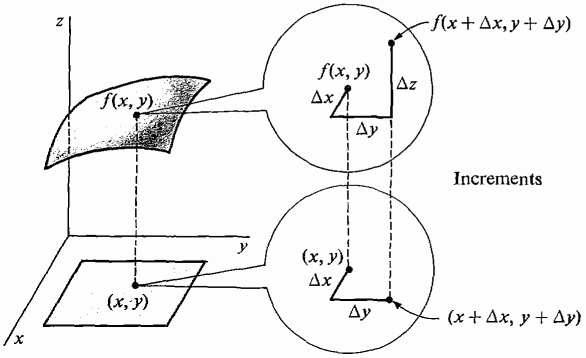
\includegraphics[width=0.5\textwidth]{fig_multi_var_11}
	\caption{Understanding the total differential of a function of two variables.}
	\label{fig_multi_var_11}
	\end{center}
\end{figure}

\ifanalysis\pagebreak\fi
\begin{definition}[Total differential]\label{def:total_differential}
Let $z=f(x,y)$ be continuous on a set $S$. Let $dx$ and $dy$ represent changes in $x$ and $y$, respectively. Where the partial derivatives $f_x$ and $f_y$ exist, the \textbf{total differential of $z$} (\textit{totale differentiaal van $z$}) is \index{total differential}\index{partial derivative!total differential}\index[aut]{totale differentiaal}\index[aut]{differentiaal ! totale}
$$dz = f_x(x,y)dx + f_y(x,y)dy.$$
\end{definition}

Note that from  Definition \ref{def:total_differential}, we can as well use vector notation: $$dz = \left(\, f_x,f_y\right)\cdot\left( dx,dy\right).$$

\subsection{Differentiability}
\subsubsection{Definition}
We can approximate $\ddz$ with $dz$, but as with all approximations, there is error involved. A good approximation is one in which the error is small. At a given point $(x_0,y_0)$, let $E_x$ and $E_y$ be functions of $dx$ and $dy$ such that $E_xdx+E_ydy$ describes this error. Then
\begin{align*}
\ddz &= dz + E_xdx+ E_ydy \\
		&= f_x(x_0,y_0)dx+f_y(x_0,y_0)dy + E_xdx+E_ydy.
\end{align*}
If the approximation of $\ddz$ by $dz$ is good, then as $dx$ and $dy$ get small,  so does $E_xdx+E_ydy$. The approximation of $\ddz$ by $dz$ is even better if, as $dx$ and $dy$ go to 0, so do $E_x$ and $E_y$. This leads us to our definition of differentiability.

\begin{definition}[Multivariable differentiability]\label{def:multi_differentiability}
Let $z=f(x,y)$ be defined on a set $S$ containing $(x_0,y_0)$ where $f_x(x_0,y_0)$ and $f_y(x_0,y_0)$ exist. Let $dz$ be the total differential of $z$ at $(x_0,y_0)$, let $\ddz = f(x_0+dx,y_0+dy) - f(x_0,y_0)$, and let $E_x$ and $E_y$ be functions of $dx$ and $dy$  such that 
$$\ddz = dz + E_xdx + E_ydy.$$
\begin{enumerate}
	\item We say \textbf{$f$ is differentiable at $(x_0,y_0)$} (\textit{afleidbaar}) if, given $\varepsilon >0$, there is a $\delta >0$ such that if $||\left(dx,dy\right)|| < \delta$, then $||\left(E_x,E_y\right)|| < \varepsilon$. That is, as $dx$ and $dy$ go to 0, so do $E_x$ and $E_y$.
	\item	We say \textbf{$f$ is differentiable on $S$} (\textit{afleidbaar over $S$}) if $f$ is differentiable at every point in $S$. If $f$ is differentiable on $\mathbb{R}^2$, we say that $f$ is differentiable everywhere.
	\index{differentiability}\index[aut]{afleidbaarheid}\index{multivariable function!differentiability}
\end{enumerate}
\end{definition}


\begin{example}\label{ex_totaldiff1}
Show $f(x,y) = xy+3y^2$ is differentiable.

\xhrulefill{gray}{2.5pt}Solution \xhrulefill{gray}{2.5pt}

We begin by finding $f(x+dx,y+dy)$, $\ddz$, $f_x$ and $f_y$.
\begin{align*}
f(x+dx,y+dy) &= (x+dx)(y+dy) + 3(y+dy)^2 \\
						&= xy + xdy+ydx+dxdy + 3y^2+6ydy+3dy^2.
\end{align*}
$\ddz = f(x+dx,y+dy) - f(x,y)$, so
$$\ddz = xdy + ydx + dxdy + 6ydy+3dy^2.$$
It is straightforward to compute $f_x = y$ and $f_y = x+6y$. Consider once more $\ddz$:
\begin{align*}
\ddz &= xdy + ydx + dxdy + 6ydy+3dy^2 \qquad \text{ (Now reorder.)}\\
		&= ydx + xdy+6ydy+ dxdy + 3dy^2\\
		&= \underbrace{(y)}_{f_x}dx + \underbrace{(x+6y)}_{f_y}dy + \underbrace{(dy)}_{E_x}dx+\underbrace{(3dy)}_{E_y}dy\\
		&= f_xdx + f_ydy + E_xdx+E_ydy.
\end{align*}
With $E_x = dy$ and $E_y = 3dy$, it is clear that as $dx$ and $ dy$ go to 0, $E_x$ and $E_y$ also go to 0. Since this did not depend on a specific point $(x_0,y_0)$, we can say that $f(x,y)$ is differentiable for all pairs $(x,y)$ in $\mathbb{R}^2$, or, equivalently, that $f$ is differentiable everywhere. 
\end{example}

Our intuitive understanding of differentiability of functions $y=f(x)$ of one variable was that the graph of $f$ was \textbf{smooth} (\textit{glad}). A similar intuitive understanding of functions $z=f(x,y)$ of two variables is that the surface defined by $f$ is also smooth, not containing cusps, edges, breaks,  etc. The following theorem states that differentiable functions are continuous, followed by another theorem that   provides a
more tangible way of determining whether a great number of functions are differentiable or not.

\begin{theorem}[Continuity and differentiability of multivariable functions]\label{thm:diff_cont_multi}
Let $z=f(x,y)$ be defined on a set $S$ containing $(x_0,y_0)$. 
If $f$ is differentiable at $(x_0,y_0)$, then $f$ is continuous at $(x_0,y_0)$.
\index{multivariable function!differentiability}\index{multivariable function!continuity}\index[aut]{continu\"iteit}
\end{theorem}

\begin{theorem}[Differentiability of multivariable functions]\label{thm:differentiable}
Let $z=f(x,y)$ be defined on a set $S$. 
If $f_x$ and $f_y$ are both continuous on $S$, then $f$ is differentiable on $S$.
\index{multivariable function!differentiability}\index[aut]{afleidbaarheid}
\end{theorem}

%\ifanalysis
%
%Bewijs toevoegen
%
%\fi
These theorems assure us that  essentially all functions that we see in the course of our studies here are differentiable (and hence continuous) on their natural domains. There is a difference between Definition \ref{def:multi_differentiability} and Theorem \ref{thm:differentiable}, though: it is possible for a function $f$ to be differentiable yet $f_x$ and/or $f_y$ is not continuous. 
So when $f_x$ and $f_y$  exist at a point but are not continuous at that point, we need to use other methods to determine whether or not $f$ is differentiable at that point.

For instance, consider the function 
$$f(x,y) = \left\{\begin{array}{ll} \dfrac{xy}{x^2+y^2}, & \quad  (x,y)\neq (0,0), \\
0, & \quad (x,y) = (0,0),\end{array}\right.$$
We can find $f_x(0,0)$ and $f_y(0,0)$ using Definition 	\ref{def:partial_derivative}:
\begin{align*}
f_x(0,0) &= \lim_{h\to 0} \frac{f(0+h,0) - f(0,0)}{h} \\[0.2cm]
				&= \lim_{h\to 0} \frac{0}{h^2} = 0;\\[0.2cm]
f_y(0,0) &= \lim_{h\to 0} \frac{f(0,0+h) - f(0,0)}{h} \\[0.2cm]
				&= \lim_{h\to 0} \frac{0}{h^2} = 0.
\end{align*}
Both $f_x$ and $f_y$ exist at $(0,0)$, but they are not continuous at $(0,0)$, as 
$$f_x(x,y) = \frac{y(y^2-x^2)}{(x^2+y^2)^2} \qquad \text{and}\qquad f_y(x,y) = \frac{x(x^2-y^2)}{(x^2+y^2)^2} $$ are not continuous at $(0,0)$. Take the limit of $f_x$ as $(x,y)\to(0,0)$ along the $x$- and $y$-axes; they give different results. So even though $f_x$ and $f_y$ exist at every point in the $xy$-plane, they are not continuous. Therefore it is possible, by Theorem \ref{thm:differentiable}, for $f$ to not be differentiable.

 Indeed, it is not. One can show that $f$ is not continuous at $(0,0)$ (see Example \ref{ex_multilimit4}), and by Theorem \ref{thm:diff_cont_multi}, this means $f$ is not differentiable at $(0,0)$.\\
														
\subsubsection{Approximating with differentials}

By the definition, when $f$ is differentiable $dz$ is a good approximation for $\ddz$ when $dx$ and $dy$ are small. We give a simple example of how this is used here.  We can use this to approximate error propagation; that is, if the input is a little off from what it should be, how far from correct will the output be? We demonstrate this in an example.

\begin{example}\label{ex_totaldiff4}
A cylindrical steel storage tank is to be built that is 10m tall and 4m across in diameter. It is known that the steel will expand/contract with temperature changes; is the overall volume of the tank more sensitive to changes in the diameter or in the height of the tank?

\xhrulefill{gray}{2.5pt}Solution \xhrulefill{gray}{2.5pt}

A cylindrical solid with height $h$ and radius $r$ has volume $V = \pi r^2h$. We can view $V$ as a function of two variables, $r$ and $h$. We can compute partial derivatives of $V$:
$$\frac{\partial V}{\partial r} = V_r(r,h) = 2\pi rh \qquad \text{and}\qquad \frac{\partial V}{\partial h} = V_h(r,h) = \pi r^2.$$
The total differential is $dV = (2\pi rh)dr + (\pi r^2)dh.$ When $h = 10$ and $r = 2$, we have \\ $dV = 40\pi dr + 4\pi dh$.
Note that the coefficient of $dr$ is $40\pi\approx 125.7$; the coefficient of $dh$ is a tenth of that, approximately $12.57$. A small change in radius will be multiplied by 125.7, whereas a small change in height will be multiplied by 12.57. Thus the volume of the tank is more sensitive to changes in radius than in height.
\end{example}


The previous example showed that the volume of a particular tank was more sensitive to changes in radius than in height. Keep in mind that this analysis only applies to a tank of those dimensions. A tank with a height of 0.3 m and radius of 5 m would be more sensitive to changes in height than in radius. One could make a chart of small changes in radius and height and find exact changes in volume given specific changes. %While this provides exact numbers, it does not give as much insight as the error analysis using the total differential.

\ifcalculus
\subsection{Functions of three variables}


The definition of differentiability for functions of three variables is very similar to that of functions of two variables. We again start with the total differential.

\begin{definition}[Total differential]\label{def:total_differential3}
Let $w=f(x,y,z)$ be continuous on a set $D$. Let $dx$, $dy$ and $dz$ represent changes in $x$, $y$ and  $z$, respectively. Where the partial derivatives $f_x$, $f_y$ and $f_z$ exist, the \textbf{total differential of $w$} is
\index{total differential}\index{partial derivative!total differential}\index[aut]{totale differentiaal}\index[aut]{differentiaal ! totale}
$$dw = f_x(x,y,z)dx + f_y(x,y,z)dy+f_z(x,y,z)dz.$$
\end{definition}

This differential can be a good approximation of the change in $w$ when $w = f(x,y,z)$ is differentiable.

\begin{definition}[Multivariable differentiability]\label{def:multi_differentiability3}
Let $w=f(x,y,z)$ be defined on a set $D$ containing $(x_0,y_0,z_0)$ where $f_x(x_0,y_0,z_0)$, $f_y(x_0,y_0,z_0)$ and $f_z(x_0,y_0,z_0)$ exist. Let $dw$ be the total differential of $w$ at $(x_0,y_0,z_0)$, let $\Delta w = f(x_0+dx,y_0+dy,z_0+dz) - f(x_0,y_0,z_0)$, and let $E_x$, $E_y$ and $E_z$ be functions of $dx$, $dy$ and $dz$  such that
\index{differentiable}\index{derivative!multivariable differentiability}\index{multivariable function!differentiability}\index[aut]{afleidbaarheid}
$$\Delta w = dw + E_xdx + E_ydy + E_zdz.$$
\begin{enumerate}
	\item We say $f$ is differentiable at $(x_0,y_0,z_0)$ if, given $\varepsilon >0$, there is a $\delta >0$ such that if $||\left(dx,dy,dz\right)|| < \delta$, then $||\left(E_x,E_y,E_z\right)|| < \varepsilon$. 
	\item	We say $f$ is differentiable on $B$ if $f$ is differentiable at every point in $B$. If $f$ is differentiable on $\mathbb{R}^3$, we say that $f$ is differentiable everywhere.
\end{enumerate}
\end{definition}

Just as before, this definition gives a rigorous statement about what it means to be differentiable that is not very intuitive. We follow it with a theorem similar to Theorem \ref{thm:differentiable}.

\ifcalculus\pagebreak\fi
\begin{theorem}[Continuity and differentiability of functions of three variables]\label{thm:differentiable3}
Let $w=f(x,y,z)$ be defined on a set $D$ containing $(x_0,y_0,z_0)$. 
\begin{enumerate}
\item	If $f$ is differentiable at $(x_0,y_0,z_0)$, then $f$ is continuous at $(x_0,y_0,z_0)$.
\item If $f_x$, $f_y$  and $f_z$ are continuous on $D$, then $f$ is differentiable on $D$.
\index{multivariable function!differentiability}\index{multivariable function!continuity}\index[aut]{afleidbaarheid}\index[aut]{continu\"iteit}
\end{enumerate}
\end{theorem}
\fi


\ifanalysis
\subsection{Functions of $n$ variables}


The definition of differentiability for functions of $n$ variables is very similar to that of functions of two variables. We again start with the total differential.

\begin{definition}[Total differential]\label{def:total_differential3}
Let $w=f(\mathbf{x})$ be continuous on a set $D$. Let $dx_i$ represent change in $x_i$. Where the partial derivatives $f_i$, $i=1,\ldots,n$, exist, \textbf{the total differential of $w$} is
\index{total differential}\index{partial derivative!total differential}\index[aut]{totale differentiaal}\index[aut]{differentiaal ! totale}
$$dw = \ds\sum\limits_{i=1}^nf_{x_i}(\mathbf{x})dx_i.$$
\end{definition}

Of course, assuming that we stick to the same increments $dx_i$, it is relatively straightforward to see that we can extend this definition to higher-order differentials.


\begin{definition}[The $n$-th order total differential]\label{def:total_differential4}
Let $w=f(\mathbf{x})$ be continuous on a set $D$. Let $dx_i$ represent change in $x_i$. Where the partial derivatives $f_i$, $i=1,\ldots,n$, exist, \textbf{the $n$-th order total differential of $w$} is
\index{total differential}\index{partial derivative!total differential}\index[aut]{totale differentiaal}\index[aut]{differentiaal ! totale}
$$d^n w =\left( \ds\sum\limits_{i=1}^nf_{x_i}(\mathbf{x})dx_i\right)^n.$$
\end{definition}

To understand this definition correctly, it is important to realize that $\frac{\partial^n}{\partial x_i^n}$ represents the $n$-th power of $\frac{\partial}{\partial x_i}$ when expanding the power $n$ according to the binomial theorem. 

The first-order total differential given in Definition~\ref{def:total_differential3} can be a good approximation of the change in $w$ when $w = f(\mathbf{x})$ is differentiable.

\begin{definition}[Multivariable differentiability]\label{def:multi_differentiability3}
Let $w=f(\mathbf{x})$ be defined on a set $D$ containing $\mathbf{c}$ where $f_{x_i}(\mathbf{c})$, $i=1,\ldots,n$ exist. Let $dw$ be the total differential of $w$ at $\mathbf{c}$, let $\Delta w = f(c_1+dx_1,c_2+dx_2,\ldots,c_n+dx_n) - f(c_1,c_2, \ldots, c_n)$ \\$=f(\mathbf{c}+\mathbf{dx}) - f(\mathbf{c})$, and let $E_{x_i}$ be functions of $dx_i$ for $i=1,\ldots,n$  such that
\index{differentiable}\index{derivative!multivariable differentiability}\index{multivariable function!differentiability}\index[aut]{afleidbaarheid}
$$\Delta w = dw + \ds\sum\limits_{i=1}^nE_{x_i}dx_i.$$
\begin{enumerate}
	\item We say \textbf{$f$ is differentiable at $\mathbf{c}$} if, given $\varepsilon >0$, there is a $\delta >0$ such that if $||\mathbf{dx}|| < \delta$, then $||\mathbf{E_x}|| < \varepsilon$. 
	\item	We say $f$ is differentiable on $B$ if $f$ is differentiable at every point in $B$. If $f$ is differentiable on $\mathbb{R}^n$, we say that $f$ is differentiable everywhere.
\end{enumerate}
\end{definition}

Just as before, this definition gives a rigorous statement about what it means to be differentiable that is not very intuitive. We follow it with a theorem similar to Theorem \ref{thm:differentiable}.

\begin{theorem}[Continuity and differentiability of functions of three variables]\label{thm:differentiable3}
Let $w=f(\mathbf{x})$ be defined on a set $D$ containing $\mathbf{c}$. 
\begin{enumerate}
\item	If $f$ is differentiable at $\mathbf{c}$, then $f$ is continuous at $\mathbf{c}$.
\item If the $f_{x_i}$, $i=1,\ldots,n$ are continuous on $B$, then $f$ is differentiable on $B$.
\index{multivariable function!differentiability}\index{multivariable function!continuity}\index[aut]{afleidbaarheid}\index[aut]{continu\"iteit}
\end{enumerate}
\end{theorem}






\fi

\ifcalculus\section{The multivariable chain rule}\label{sec:multi_chain}\fi
\ifanalysis\section{The multivariable chain rule and  implicit function theorem}\label{sec:multi_chain}\fi
\subsection{Rationale}
Consider driving an off-road vehicle along a dirt road. As you drive, your elevation likely changes. What factors determine how quickly your elevation rises and falls? 
After some thought, generally one recognizes that one's velocity (speed and direction) and the terrain influence your rise and fall. 

One can represent the terrain as the surface defined by a multivariable function $z=f(x,y)$; one can represent the path of the off-road vehicle, as seen from above, with a vector--valued function \linebreak $\vec r(t) = \left( x(t), y(t)\right)$; the velocity of the vehicle is thus $\vrp(t) = \left( x'(t),y'(t)\right)$.

Consider Figure \ref{fig_multi_var_12} in which a surface $z=f(x,y)$ is drawn, along with a dashed curve in the $xy$-plane. Restricting $f$ to just the points on this circle gives the curve shown on the surface (i.e., the path of the vehicle.) The derivative $\frac{df}{dt}$ gives the instantaneous rate of change of $f$ with respect to $t$. If we consider an object travelling along this path, $\frac{df}{dt}=\frac{dz}{dt}$ gives the rate at which the object rises/falls. Conceptually, the multivariable chain rule combines terrain and velocity information properly to compute this rate of elevation change. 



\begin{figure}
	\begin{center}
			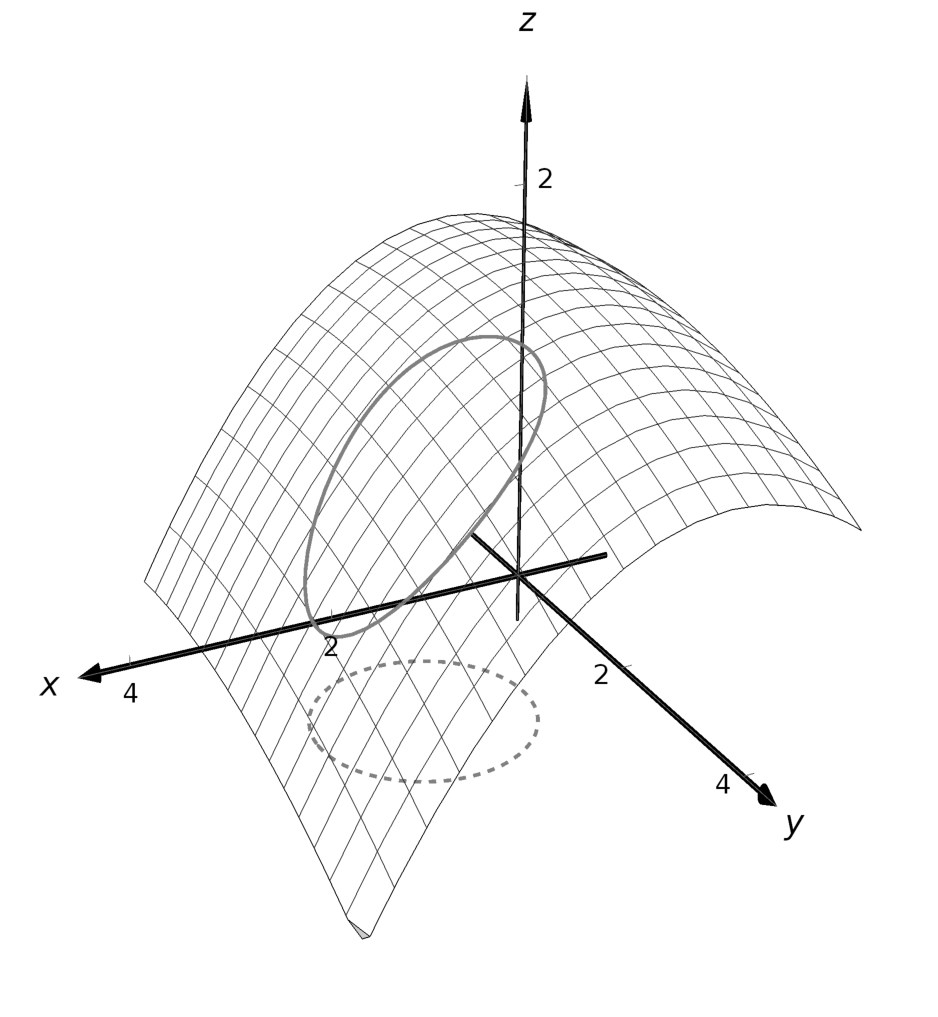
\includegraphics[width=0.5\textwidth]{fig_multi_var_12}
	\caption{Understanding the application of the multivariable chain rule.}
	\label{fig_multi_var_12}
	\end{center}
\end{figure}


Abstractly, let $z$ be a function of $x$ and $y$; that is, $z=f(x,y)$ for some function $f$, and let $x$ and $y$ each be functions of $t$. By choosing a $t$-value, $x$- and $y$-values are determined, which in turn determine $z$: this defines $z$ as a function of $t$. The multivariable chain rule gives a method of computing $ \frac{dz}{dt}$.


\begin{theorem}[Multivariable chain rule, Part I]\label{thm:multi_chain}
Let $z=f(x,y)$, $x=g(t)$ and $y=h(t)$, where $f$, $g$ and $h$ are differentiable functions. Then \linebreak $z = f(x,y) = f\big(g(t),h(t)\big)$ is a function of $t$, and 
\index{derivative!chain rule}\index{chain rule}\index[aut]{kettingregel}\index[aut]{afgeleide ! kettingregel}
\begin{align}
\frac{dz}{dt} = \frac{df}{dt} &= f_x(x,y)\frac{dx}{dt}+f_y(x,y)\frac{dy}{dt}\nonumber\\[5pt]
		&= \frac{\partial f}{\partial x}\frac{dx}{dt}+\frac{\partial f}{\partial y}\frac{dy}{dt}\label{ketting1}\\[0.2cm]
		&= \left( f_x,f_y\right) \cdot \left( x',y'\right).\nonumber
\end{align}
\end{theorem}

\ifanalysis

Although this theorem should be clear if one has a good understanding of the chain rule, which forces you to work from outer function to the inner one, it can be shown more formally, for instance, by resorting to Definition~\ref{def:total_differential}, which allows us to write that
$$dz = f_x(x,y)\,dx+f_y(x,y)\,dy\,.$$
Dividing both sides by $dt$ and recalling that $x=g(t)$ and $y=h(t)$ are differentiable functions, we get
$$
\dfrac{dz}{dt}=\frac{\partial f}{\partial x}\frac{dx}{dt}+\frac{\partial f}{\partial y}\frac{dy}{dt}\,.
$$

\fi
Notice, the third line of equations in Theorem \ref{thm:multi_chain}. The vector $\left(f_x,f_y\right)$ contains information about the surface (terrain); the vector $\left( x',y'\right)$ can represent velocity. In the context measuring the rate of elevation change of the off-road vehicle, the multivariable chain rule states it can be found through a product of terrain and velocity information.


We now practice applying the multivariable chain rule.


\begin{example}\label{ex_mchain1}
Let $z=f(x,y)=x^2y+x$, where $x=\sin(t)$ and $y=e^{5t}$. Find $ \frac{dz}{dt}$ using the chain rule.

\xhrulefill{gray}{2.5pt}Solution \xhrulefill{gray}{2.5pt}

Following Theorem \ref{thm:multi_chain}, we first find
$$f_x(x,y) = 2xy+1,\qquad f_y(x,y) = x^2,\qquad \frac{dx}{dt} = \cos(t),\qquad \frac{dy}{dt}= 5e^{5t}.$$
Applying the theorem, we have
$$\frac{dz}{dt} = (2xy+1)\cos(t) + 5x^2e^{5t}.$$
This may look odd, as it seems that $\frac{dz}{dt}$ is a function of $x$, $y$ and $t$. Since $x$ and $y$ are functions of $t$, $\frac{dz}{dt}$ is really just a function of $t$, and we can replace $x$ with $\sin(t)$ and $y$ with $e^{5t}$ to arrive of:
$$\frac{dz}{dt} = (2\sin (t)e^{5t}+1)\cos(t) + 5e^{5t}\sin^2(t).$$
\end{example}

The previous example can make us wonder: if we substituted for $x$ and $y$ at the end to show that $\frac{dz}{dt}$ is really just a function of $t$, why not substitute before differentiating, showing clearly that $z$ is a function of $t$?

That is, $z = x^2y+x = \sin^2(t)e^{5t}+\sin(t).$ Applying the chain and product rules, we have 
$$\frac{dz}{dt} = 2\sin(t)\cos(t)\, e^{5t}+ 5\sin^2(t)\,e^{5t}+\cos(t),$$ which matches the result from the example.

This may now make one wonder ``What's the point? If we could already find the derivative, why learn another way of finding it?'' In some cases, applying this rule makes deriving simpler, but this is hardly the power of the chain rule. Rather, in the case where $z=f(x,y)$, $x=g(t)$ and $y=h(t)$, the chain rule is extremely powerful when we do not know what $f$, $g$ and/or $h$ are. We demonstrate this in the next example.

\begin{example}\label{ex_mchain100}
An object travels along a path on a surface. The exact path and surface are not known, but at time $t=t_0$ it is known that :
$$\frac{\partial z}{\partial x} = 5,\qquad \frac{\partial z}{\partial y}=-2,\qquad \frac{dx}{dt}=3\qquad \text{and}\qquad \frac{dy}{dt}=7.$$
Find $\frac{dz}{dt}$ at time $t_0$.

\xhrulefill{gray}{2.5pt}Solution \xhrulefill{gray}{2.5pt}

The multivariable chain rule states that 
\begin{align*}
\frac{dz}{dt} &= \frac{\partial z}{\partial x}\frac{dx}{dt} + \frac{\partial z}{\partial y}\frac{dy}{dt} \\
				&= 5(3)+(-2)(7) \\
				&=1.
\end{align*}
By knowing certain rates--of--change information about the surface and about the path of the particle in the $xy$-plane, we can determine how quickly the object is rising/falling. 
\end{example}

\ifanalysis
Of course, we might as well be interested in the second derivative of $z=f(x,y)$. To compute that derivative, it is important to realize that one again gets a function of $t$ upon substituting $x=g(t)$ and $y=h(t)$ in the right-hand side of Equation~\eqref{ketting1}. So we may compute
$$
\frac{d^2z}{dt^2}=\frac{d}{dt}\left(\frac{\partial f}{\partial x}\frac{dx}{dt}+\frac{\partial f}{\partial y}\frac{dy}{dt}\right)\,.
$$
Applying the product rule, we get
$$
\frac{d^2z}{dt^2}=\frac{d}{dt}\left(\frac{\partial f}{\partial x}\right)\frac{dx}{dt}+\frac{\partial f}{\partial x}\frac{d^2x}{dt^2}+\frac{d}{dt}\left(\frac{\partial f}{\partial y}\right)\frac{dy}{dt}+\frac{\partial f}{\partial y}\frac{d^2y}{dt^2}\,, 
$$
and after expanding the derivatives in the first and third term:
$$
\frac{d^2z}{dt^2}=\left(\frac{\partial^2 f}{\partial x^2}\frac{dx}{dt}+\frac{\partial^2 f}{\partial y\partial x}\frac{dy}{dt}\right)\frac{dx}{dt}+\frac{\partial f}{\partial x}\frac{d^2x}{dt^2}+\left(\frac{\partial^2 f}{\partial x\partial y}\frac{dx}{dt}+\frac{\partial^2 f}{\partial y^2}\frac{dy}{dt}\right)\frac{dy}{dt}+\frac{\partial f}{\partial y}\frac{d^2y}{dt^2}.
$$
After simplification, we arrive at
$$
\frac{d^2z}{dt^2}=\frac{\partial^2 f}{\partial x^2}\left(\frac{dx}{dt}\right)^2+2\frac{\partial^2 f}{\partial x\partial y}\frac{dx}{dt}\frac{dy}{dt}+\frac{\partial^2 f}{\partial y^2}\left(\frac{dy}{dt}\right)^2+\frac{\partial f}{\partial x}\frac{d^2x}{dt^2}+\frac{\partial f}{\partial y}\frac{d^2y}{dt^2}\,,
$$
which we can write as
$$
\frac{d^2z}{dt^2}=\left(\frac{\partial }{\partial x}\frac{dx}{dt}+\frac{\partial }{\partial y}\frac{dy}{dt}\right)^2f+\frac{\partial f}{\partial x}\frac{d^2x}{dt^2}+\frac{\partial f}{\partial y}\frac{d^2y}{dt^2}\,.
$$

A similar reasoning is possible for higher-order derivatives. Note that, again, just as in Definition~\ref{def:total_differential4},  $\left(\frac{\partial}{\partial x}\right)^2$ is to be understood as $\frac{\partial^2}{\partial x^2}$.

\fi 
We can also extend the chain rule to include the situation where $z$ is a function of more than one variable, and each of these variables is also a function of more than one variable. The basic case of this is where $z=f(x,y)$, and $x$ and $y$ are functions of two variables, say $s$ and $t$. \\

\ifcalculus
\begin{theorem}[Multivariable chain rule, Part II]\label{thm:multi_chain2}
\begin{enumerate}
	\item Let $z=f(x,y)$, $x=g(s,t)$ and $y=h(s,t)$, where $f$, $g$ and $h$ are differentiable functions. Then $z$ is a function of $s$ and $t$, and
		\begin{multicols}{2}
			$\ds \frac{\partial z}{\partial s} = \frac{\partial f}{\partial x}\frac{\partial x}{\partial s} + \frac{\partial f}{\partial y}\frac{\partial y}{\partial s}$\\
			$\ds \frac{\partial z}{\partial t} = \frac{\partial f}{\partial x}\frac{\partial x}{\partial t} + \frac{\partial f}{\partial y}\frac{\partial y}{\partial t}$
			\end{multicols}
			\index{derivative!Chain Rule}\index{Chain Rule!multivariable}

		
		\item		Let $w = f(x,y,z)$ be a differentiable function of three variables, where $x, y$ and $z$ are differentiable functions of the variables $t_1,t_2,\ldots,t_n$. Then $w$ is a function of the $t_i$, and 
		$$\frac{\partial z}{\partial t_i} = \frac{\partial f}{\partial x}\frac{\partial x}{\partial t_i} + \frac{\partial f}{\partial y}\frac{\partial y}{\partial t_i} +  \frac{\partial f}{\partial z}\frac{\partial z}{\partial t_i}.$$
\end{enumerate}
\end{theorem}
\fi


\ifanalysis
\begin{theorem}[Multivariable chain rule, Part II]\label{thm:multi_chain2}

\begin{enumerate}
	\item Let $z=f(x,y)$, $x=g(s,t)$ and $y=h(s,t)$, where $f$, $g$ and $h$ are differentiable functions. Then $z$ is a function of $s$ and $t$, and
		\begin{multicols}{2}
			$\ds \frac{\partial z}{\partial s} = \frac{\partial f}{\partial x}\frac{\partial x}{\partial s} + \frac{\partial f}{\partial y}\frac{\partial y}{\partial s}$\\
			$\ds \frac{\partial z}{\partial t} = \frac{\partial f}{\partial x}\frac{\partial x}{\partial t} + \frac{\partial f}{\partial y}\frac{\partial y}{\partial t}.$
			\end{multicols}
			\index{derivative!Chain Rule}\index{Chain Rule!multivariable}
		%\end{itemize}
		
		\item		Let $z = f(\mathbf{x})$ be a differentiable function of $n$ variables, where each of the $x_i$ is a differentiable function of the variables $t_1,t_2,\ldots,t_n$. Then $z$ is a function of the $t_j$, and 
		$$\frac{\partial z}{\partial t_j} = \sum\limits_{i=1}^n\frac{\partial f}{\partial x_i}\frac{\partial x_i}{\partial t_j}.$$
\end{enumerate}

\end{theorem}
\fi

\begin{example}\label{ex_mchain3}
Let $z=f(x,y)=x^2y+x$, $x=s^2+3t$ and $y=2s-t$. Find $\frac{\partial z}{\partial s}$ and $\frac{\partial z}{\partial t}$, and evaluate each when $s=1$ and $t=2$.

\ifcalculus\pagebreak\fi
\xhrulefill{gray}{2.5pt}Solution \xhrulefill{gray}{2.5pt}

Following Theorem \ref{thm:multi_chain2}, we compute the following partial derivatives:
$$\frac{\partial f}{\partial x} = 2xy+1\qquad\qquad \frac{\partial f}{\partial y} = x^2,$$
$$\frac{\partial x}{\partial s} = 2s \qquad\qquad \frac{\partial x}{\partial t} = 3\qquad\qquad \frac{\partial y}{\partial s} = 2 \qquad\qquad \frac{\partial y}{\partial t} = -1.$$
Thus 
$$\ds \frac{\partial z}{\partial s}=\frac{\partial f}{\partial x}\frac{\partial x}{\partial s} +\frac{\partial f}{\partial y}\frac{\partial y}{\partial s}= (2xy+1)(2s) + (x^2)(2) = 4xys+2s + 2x^2,$$
and
$$\ds \frac{\partial z}{\partial t}=\frac{\partial f}{\partial x}\frac{\partial x}{\partial t} +\frac{\partial f}{\partial y}\frac{\partial y}{\partial t} = (2xy+1)(3) + (x^2)(-1) = 6xy-x^2+3.$$
When $s=1$ and $t=2$, $x= 7$ and $y= 0$, so 
$$\frac{\partial z}{\partial s} = 100\qquad \text{and}\qquad \frac{\partial z}{\partial t} = -46.$$
\end{example}

\begin{example}\label{ex_mchain4}
Let $w = xy+z^2$, where $x= t^2e^s$, $y= t\cos(s)$, and $z=s\sin(t)$. Find $\frac{\partial w}{\partial t}$ when $s=0$ and $t=\pi$.

\xhrulefill{gray}{2.5pt}Solution \xhrulefill{gray}{2.5pt}

Following Theorem \ref{thm:multi_chain2}, we compute the following partial derivatives:
$$\frac{\partial f}{\partial x} = y\qquad\qquad \frac{\partial f}{\partial y} = x\qquad\qquad \frac{\partial f}{\partial z} = 2z,$$
$$\frac{\partial x}{\partial t} = 2te^s\qquad\qquad \frac{\partial y}{\partial t} = \cos (s)\qquad\qquad \frac{\partial z}{\partial t} = s\cos (t).$$
Thus $$\ds \frac{\partial w}{\partial t} = y(2te^s) + x(\cos(s)) + 2z(s\cos(t)).$$ 
When $s=0$ and $t=\pi$, we have $x=\pi^2$, $y=\pi$ and $z=0$. Thus
$$\frac{\partial w}{\partial t} = \pi(2\pi) + \pi^2 = 3\pi^2.$$
\end{example}


\ifanalysis

As indicated before, the real strength of the multivariable chain rule lies in the fact that one can compute derivatives and differentials of multivariable functions even not knowing the underlying function definitions. This is illustrated in the following example.

\begin{example}

In each of the following cases, determine $dz$ and $d^2z$
\begin{multicols}{2}
\begin{enumerate}
\item $z=f(u)$ and $u=g(x,y)$
\item  $z=f(u,v)$, $u=g(x,y)$ and $v=h(x,y)$
\end{enumerate}
\end{multicols}

\xhrulefill{gray}{2.5pt}Solution \xhrulefill{gray}{2.5pt}

\begin{enumerate}
\item \begin{enumerate}
\item \begin{tabbing}
$dz \;\; $\= $ = \;\; \ds\frac{\partial z}{\partial x} \; dx + \ds\frac{\partial z}{\partial y} \; dy $\\[0.2cm]
\> $ = \;\;\ds\frac{d f}{d u}\;\ds\frac{\partial u}{\partial x} \; dx+\ds\frac{df}{du}\ds\frac{\partial u}{\partial y}\; dy$\\[0.2cm]
\>$ = \;\;\ds\frac{d f}{d u}\; \left [\ds\frac{\partial u}{\partial x} \; dx + \ds\frac{\partial u}{\partial y} \; dy \right ]$\\[0.2cm]
\>$ = \;\ds\frac{d f}{d u}\; du$
\end{tabbing}
\item[]
\item \begin{tabbing}
$d^2 z \;\; $\= $ = \;\; \ds\frac{\partial^2 z}{\partial x^2} \; dx^2 + 2 \ds\frac{\partial^2 z}{\partial x \partial y}\;   dx \; dy + \ds\frac{\partial^2 z}{\partial y^2} \; dy^2$\\[0.2cm]
\>$ = \;\; \left [ \ds\frac{d^2 f}{d u^2} \; \left(\ds\frac{\partial u}{\partial x} \right)^2  + \ds\frac{d f}{d u}\; \ds\frac{\partial^2 u}{\partial x^2} \right] \; dx^2 +  2 \left[ \ds\frac{d^2 f}{d u^2} \; \ds\frac{\partial u}{\partial x} \;\ds\frac{\partial u}{\partial y} + \ds\frac{d f}{d u}\;\ds\frac{\partial^2 u}{\partial x \partial y} \; \right ] dx \; dy
$\\[0.2cm]
\> \hspace{7.5cm} $ + \left[\ds\frac{d^2 f}{d u^2} \; \left(\ds\frac{\partial u}{\partial y} \right)^2  + \ds\frac{d f}{d u}\; \ds\frac{\partial^2 u}{\partial y^2} \right] \; dy^2$\\[0.2cm]
\>$ = \;\; \ds\frac{d^2 f}{du^2} \; \left[\ds\frac{\partial u}{\partial x} \; dx +  \ds\frac{\partial u}{\partial y} \; dy \right]^2+ \ds\frac{d f}{du} \; \left[\ds\frac{\partial }{\partial x} \; dx +  \ds\frac{\partial }{\partial y} \; dy \right]^2 \; u $\\[0.2cm]
\> $ = \;\;  \ds\frac{d^2 f}{d u^2}\; du^2 +  \ds\frac{d f}{d u}\; d^2 u$
\end{tabbing}
\end{enumerate}
\item 
\begin{enumerate}
\item \begin{tabbing}
$dz \;\; $\= $ = \;\; \ds\frac{\partial z}{\partial x} \; dx + \ds\frac{\partial z}{\partial y} \; dy $\\[0.18cm]
\> $ = \;\;  \left( \ds\frac{\partial f}{\partial u}  \; \ds\frac{\partial u}{\partial x} + \ds\frac{\partial f}{\partial v}  \; \ds\frac{\partial v}{\partial x}\right) \; dx + \left(\ds\frac{\partial f}{\partial u}  \; \ds\frac{\partial u}{\partial y} +\ds\frac{\partial f}{\partial v}  \; \ds\frac{\partial v}{\partial y}\right) \; dy$\\[0.18cm]
\> $ = \;\; \ds\frac{\partial f}{\partial u}  \; \left(\ds\frac{\partial u}{\partial x} \; dx + \ds\frac{\partial u}{\partial y} \; dy \right ) + \ds\frac{\partial f}{\partial v}  \; \left( \ds\frac{\partial v}{\partial x} \;  dx
+  \ds\frac{\partial v}{\partial y} \; dy \right)$\\[0.18cm]
\> $ = \;\; \ds\frac{\partial f}{\partial u}  \; du + \ds\frac{\partial f}{\partial v} \; dv $
\end{tabbing}
\item[]
\item \begin{tabbing}
$d^2 z \;\; $\= $ = \;\; \ds\frac{\partial^2 z}{\partial x^2} \; dx^2 + 2 \; \ds\frac{\partial^2 z}{\partial x \partial y}  \; dx \; dy + \ds\frac{\partial^2 z}{\partial y^2} \; dy^2$\\[0.18cm]
\>$ = \;\; \left[\ds\frac{\partial^2 f}{\partial u^2} \left(\ds\frac{\partial u}{\partial x} \right)^2 + 2\; \ds\frac{\partial^2 f}{\partial u \partial v}\ds\frac{\partial u}{\partial x}\ds\frac{\partial v}{\partial x}+
\ds\frac{\partial^2 f}{\partial v^2} \; \left(\ds\frac{\partial v}{\partial x} \right )^2+\ds\frac{\partial f}{\partial u}
\ds\frac{\partial^2 u}{\partial x^2} +\ds\frac{\partial f}{\partial v}\ds\frac{\partial^2 v}{\partial x^2}\right]\; dx^2
$\\[0.18cm]
\> $ \hspace{0.7cm} +\; 2 \left[\ds\frac{\partial^2 f}{\partial u^2}\;\ds\frac{\partial u}{\partial x} \;\ds\frac{\partial u}{\partial y}+\ds\frac{\partial^2 f}{\partial u \partial v} \;\ds\frac{\partial u}{\partial x} \;\ds\frac{\partial v}{\partial y}+ \ds\frac{\partial^2 f}{\partial u \partial v}\;\ds\frac{\partial u}{\partial y}\;\ds\frac{\partial v}{\partial x}\right.$\\[0.18cm]
\>$ \left. \hspace{5.3cm} +\;
%\ds\frac{\partial^2 f}{\partial u^2} \;
%\ds\frac{\partial u}{\partial y}\;
%\ds\frac{\partial v}{\partial x}
\ds\frac{\partial^2 f}{\partial v^2}\;\ds\frac{\partial v}{\partial x} \;\ds\frac{\partial v}{\partial y}\;+
\ds\frac{\partial f}{\partial u}\ds\frac{\partial^2 u}{\partial x \partial y}+\ds\frac{\partial f}{\partial v}\ds\frac{\partial^2 v}{\partial x \partial y}\right] \; dx dy $\\[0.18cm]
\> $ \hspace{0.7cm} + \left[\ds\frac{\partial^2 f}{\partial u^2} \left(\ds\frac{\partial u}{\partial y} \right)^2+ 2 \ds\frac{\partial^2 f}{\partial u \partial v}\ds\frac{\partial u}{\partial y} \ds\frac{\partial v}{\partial y} +
\ds\frac{\partial^2 f}{\partial v^2} \left(\ds\frac{\partial v}{\partial y} \right)^2+\ds\frac{\partial f}{\partial u}
\ds\frac{\partial^2 u}{\partial y^2} +\ds\frac{\partial f}{\partial v} \ds\frac{\partial^2 v}{\partial y^2} \right]  dy^2$\\[0.18cm]
\> $ = \;\;  \ds\frac{\partial^2 f}{\partial u^2} \left[\left(\ds\frac{\partial u}{\partial x} \right )^2 dx^2+ 2 \;
\ds\frac{\partial u}{\partial x} \;\ds\frac{\partial u}{\partial y} \; dx \; dy +\left(\ds\frac{\partial u}{\partial y} \right)^2  dy^2\right ] $\\[0.18cm]
\> $ \hspace{0.7cm} + \; 2 \; \ds\frac{\partial^2 f}{\partial u \partial v} \left[\ds\frac{\partial u}{\partial x} \;
\ds\frac{\partial v}{\partial x} \; dx^2+\ds\frac{\partial u}{\partial x} \;\ds\frac{\partial v}{\partial y} \; dx \; dy
+\ds\frac{\partial u}{\partial y} \;\ds\frac{\partial v}{\partial x} \; dx \; dy+\ds\frac{\partial u}{\partial y}\ds\frac{\partial v}{\partial y} \; dy^2\right] $\\[0.18cm] 
\> $ \hspace{0.7cm} +\;\ds\frac{\partial^2 f}{\partial v^2} \left[ \left(\ds\frac{\partial v}{\partial x} \right )^2  dx^2
+ \; 2 \;\ds\frac{\partial v}{\partial x} \;\ds\frac{\partial v}{\partial y} \;dx \; dy +\left(\ds\frac{\partial v}{\partial y} \right )^2 dy^2\right ]$\\[0.18cm]
\>$ \hspace{0.7cm} + \; \ds\frac{\partial f}{\partial u} \left[\ds\frac{\partial^2 u}{\partial x^2} \; dx^2+ 2 \; \ds\frac{\partial^2 u}{\partial x \partial y} \; dx \; dy +\ds\frac{\partial^2 u}{\partial y^2} \; dy^2\right ] $\\[0.18cm] 
\>$ \hspace{0.7cm} + \;\ds\frac{\partial f}{\partial v} \left[\ds\frac{\partial^2 v}{\partial x^2} \; dx^2
+ 2 \; \ds\frac{\partial^2 v}{\partial x \partial y} \; dx \; dy +\ds\frac{\partial^2 v}{\partial y^2} \; dy^2
\right ]$\\[0.18cm]
\>$ = \;\; \ds\frac{\partial f^2}{\partial u^2} \; du^2 + 2 \ds\frac{\partial^2 f}{\partial u \partial v}  \;   du \; dv + \ds\frac{\partial^2 f}{\partial v^2} \; dv^2 +  \ds\frac{\partial f}{\partial u} \; d^2 u +\ds\frac{\partial f}{\partial v}  \; d^2 v$\\[0.18cm]
\>$ = \;\; \left[\ds\frac{\partial }{\partial u } \; du +  \ds\frac{\partial }{\partial v} \; dv \right]^2 f
+  \ds\frac{\partial f}{\partial u} \; d^2 u +\ds\frac{\partial f}{\partial v}  \; d^2 v$
\end{tabbing}
\end{enumerate}
\end{enumerate}

\end{example}



\fi

\ifcalculus\subsection{Implicit functions}\fi
\ifanalysis\subsection{The implicit function theorem}\fi
	\checkoddpage
\marginpar{\ifoddpage\hspace*{-1.5cm}\else\hspace*{0.25cm}\fi
\includegraphics[width=0.075\textwidth]{youtube}\\
\ifoddpage\hspace*{-1.75cm}\else\hspace*{0.1cm}\fi
\qrcode[height=1.75cm]{https://youtu.be/bk9IKHS5KbY}
%\includegraphics[width=0.1\textwidth]{IFT}
}
We studied finding $\frac{dy}{dx}$ when $y$ is given as an implicit function of $x$ in detail in Section \ref{sec:imp_deriv}. We find here that the multivariable chain rule gives a simpler method of finding $\frac{dy}{dx}$.

For instance, consider the implicit function $x^2y-xy^3=3.$ We learned to use the following steps to find $\frac{dy}{dx}$:
\begin{align}
\frac{d}{dx}\Big(x^2y-xy^3\big) &= \frac{d}{dx}\Big(3\Big) \notag\\
\Rightarrow \quad  2xy + x^2\frac{dy}{dx}-y^3-3xy^2\frac{dy}{dx} &= 0\notag \\
\Leftrightarrow \quad \frac{dy}{dx} = -\frac{2xy-y^3}{x^2-3xy^2}.\label{eq:mchain2}
\end{align}

Instead of using this method, consider $z=x^2y-xy^3$. The implicit function above describes the level curve $z=3$. Considering $x$ and $y$ as functions of $x$, the multivariable chain rule states that
\begin{equation}\frac{dz}{dx} = \frac{\partial z}{\partial x}\frac{dx}{dx}+\frac{\partial z}{\partial y}\frac{dy}{dx}.\label{eq:mchain1}\end{equation}
Since $z$ is constant (in our example, $z=3$) it holds that, $\frac{dz}{dx} = 0$. We also know $\frac{dx}{dx} = 1$. Consequently, equation \eqref{eq:mchain1} becomes
\begin{align}
0 &= \frac{\partial z}{\partial x}(1) + \frac{\partial z}{\partial y}\frac{dy}{dx}. \quad \nonumber\\[5pt]
\intertext{Consequently,}
\frac{dy}{dx} &= -\frac{\partial z}{\partial x}\Big/\frac{\partial z}{\partial y} = -\frac{\,f_x\,}{f_y}\label{eq:implicit_deriv_chain}
\end{align}

Note how our solution for $\frac{dy}{dx}$ in Equation \eqref{eq:mchain2} is just the partial derivative of $z$ with respect to $x$, divided by the partial derivative of $z$ with respect to $y$, all multiplied by $(-1)$.

\ifcalculus
Actually, Equation~\eqref{eq:implicit_deriv_chain} is a consequence of the powerful implicit function theorem, which is, however, beyond the scope of this course. 
\fi

\ifanalysis

Actually, Equation~\eqref{eq:implicit_deriv_chain} is a consequence of the powerful implicit function theorem (\textit{impliciete functiestelling}), which can be formulated as follows for implicit functions of two variables $F(x,y)=0$. 

\pagebreak
\begin{theorem}[The implicit function theorem]
\label{thm:implicit1}
Let $F$ be a continuously differentiable implicit function of two variables $x$ and $y$, i.e.\ it is of differentiability  class $C^1$,  let $(x_0,y_0)$ be a point for which $F(x_0,y_0)=0$ and let 
$$
\dfrac{\partial F}{\partial y}(x_0,y_0)\neq0\,.
$$
Then there exists an open interval $I$ containing $x_0$ and a unique $C^1$ function $f:I\mapsto\mathbb{R}$ such that
$f(x_0)=y_0$ and $F(x,f(x))=0$ for all $x\in\,I$.
\end{theorem}

Essentially, the implicit function theorem allows relations 
$$\left\{(x,y)\in\mathbb{R}^2\mid F(x,y)=0\right\}$$
 to be converted to functions of a real variable. It does so by representing the relation as the graph of a function. There may, however, not be a single function whose graph can represent the entire relation, but there may be such a function on a restriction of the domain of the relation. The implicit function theorem gives a sufficient condition to ensure that there is such a function. 

\begin{example}
Let us consider  $\displaystyle F(x,y)=x^{2}+y^{2}-1=0$. We know that the equation $x^{2}+y^{2}-1=0$  cuts out the unit circle. There is no way to represent the unit circle as the graph of a function of one variable $y = f(x)$ because for each choice of $x\in[-1,1]$, there are two choices of $y$, namely $y= \pm {\sqrt {1-x^{2}}}$. It even works in situations where we do not have a formula for $F(x, y)$. 

Still, as long as $y_0\neq 0$, the conditions of Theorem~\ref{thm:implicit1} are fulfilled and we are guaranteed that there exists a unique function $f$ of one variable $x$ on $]-1,1[$ for which $f(x_0)=y_0$.   More specifically, for $-1 < x_0 < 1$ and $y_0>0$,  we let $f_{1}(x)={\sqrt {1-x^{2}}}$  and the graph of $y=f_{1}(x)$ provides the upper half of the circle. Similarly, for $-1 < x_0 < 1$ and $y_0<0$, we let $f_{2}(x)=-{\sqrt {1-x^{2}}}$ and the graph of $y=f_{2}(x)$ gives the lower half of the circle. So, it is possible to represent part of the circle as the graph of a function of one variable.

At the intersections  of the unit circle with $x$-axis, i.e.\ where $y=0$, however, we observe that 
$$
\dfrac{\partial F}{\partial y}=0\,,
$$
which implies that the conditions in Theorem~\ref{thm:implicit1} are not met and we hence may not use it. We observe that these points of intersection lie on the graphs of both $f_1$ and $f_2$ when these are extended to the closed interval $[-1,1]$.

The purpose of the implicit function theorem is to tell us the existence of functions like $f_1(x)$ and $f_2(x)$, even in situations where we cannot write them down with explicit formulas. The theorem guarantees that $f_1(x)$ and $f_2(x)$ are differentiable. For instance, for what concerns the implicit function at stake, we may take advantage of the fact that $F(x,f_i(x))=0$ as long as $y_0\neq0$ to write
\begin{eqnarray}
\dfrac{\partial F}{\partial x}+\dfrac{\partial F}{\partial y}\dfrac{df_i}{dx}&=&0\,,\label{vbimpliciet}\\[0.2cm]
\Leftrightarrow\quad2x+2y\dfrac{df_i}{dx}&=&0\,,\nonumber
\end{eqnarray}
from which we conclude that
$$
\dfrac{df_i}{dx}=-\dfrac{x}{y}\,.
$$
Consequently, we find that
$$
\dfrac{df_1}{dx}=-\dfrac{x}{\sqrt{1-x^2}}
$$
or
$$
\dfrac{df_2}{dx}=\dfrac{x}{\sqrt{1-x^2}}\,.
$$
Of course, the second-order derivatives can computed by applying the chain rule once more to Equation~\eqref{vbimpliciet} to arrive at
$$
\dfrac{\partial^2 F}{\partial x^2}+2\dfrac{\partial^2 F}{\partial x\partial y}\dfrac{df_i}{dx}+\dfrac{\partial F}{\partial y}\dfrac{d^2f_i}{dx^2}+\dfrac{\partial^2 F}{\partial y^2}\left(\dfrac{df_i}{dx}\right)^2=0\,.
$$
From this expression, it is easy to compute $\frac{d^2f_i}{dx^2}$.
\end{example}

Having introduced the implicit function theorem for functions of two variables, we now extend it to implicit functions of $n+1$ variables $F(\mathbf{x},y)$.

\begin{theorem}[The general implicit function theorem]
\label{thm:implicit2}
Let $F$ be a continuously differentiable implicit function of $n+1$ variables $\mathbf{x}=(x_1,x_2,\ldots,x_n)$ and $y$, i.e.\ it is of differentiability  class $C^1$,  let $(\mathbf{x}_0,y_0)$ be a point for which $F(\mathbf{x}_0,y_0)=0$ and let 
$$
\dfrac{\partial F}{\partial y}(\mathbf{x}_0,y_0)\neq0\,.
$$
Then there exists an open $n-$dimensional ball $B$ containing $\mathbf{x}_0$ and a unique $C^1$ function $f:B\mapsto\mathbb{R}$ such that
$f(\mathbf{x}_0)=y_0$ and $F(\mathbf{x},f(\mathbf{x}))=0$ for all $\mathbf{x}\in\,B$.
\end{theorem}

To settle the mind, let us consider one more example. 

\begin{example}
Consider the following implicit function of three variables $$
F(x,y,z)=ze^z-x-3y=0\,.
$$

Clearly, near the point $(e,0,1)$ the conditions of Theorem~\ref{thm:implicit2} are fulfilled since $F(e,0,1)=0$ and 
$$
\dfrac{\partial F}{\partial z}(e,0,1)=2e\,.
$$
So, there exists a function $z=f(x,y)$, and we may proceed by computing its first-order derivatives as follows
\begin{equation}
\begin{array}{rcl}
\dfrac{\partial F}{\partial x}+\dfrac{\partial F}{\partial z}\dfrac{\partial f}{\partial x}=-1+(z+1)e^z\dfrac{\partial f}{\partial x}&=&0,\\[0.4cm]
\dfrac{\partial F}{\partial y}+\dfrac{\partial F}{\partial z}\dfrac{\partial f}{\partial y}=-3+(z+1)e^z\dfrac{\partial f}{\partial y}&=&0,
\end{array}
\label{vbimpliciet2}
\end{equation}
from which we obtain
$$
\dfrac{\partial f}{\partial x}=\dfrac{e^{-z}}{z+1}\qquad \text{ and } \qquad
\dfrac{\partial f}{\partial y}=\dfrac{3e^{-z}}{z+1}.
$$

Taking the derivatives of the expressions in Equation~\eqref{vbimpliciet2} yields 
\begin{equation*}
\begin{array}{rcl}
(z+2)e^z\left(\dfrac{\partial f}{\partial x}\right)^2+(z+1)e^z\dfrac{\partial^2 f}{\partial x^2}&=&0,\\[0.4cm]
(z+2)e^z\dfrac{\partial f}{\partial x}\dfrac{\partial f}{\partial y}+(z+1)e^z\dfrac{\partial^2 f}{\partial x\partial y}&=&0,\\[0.4cm]
(z+2)e^z\left(\dfrac{\partial f}{\partial y}\right)^2+(z+1)e^z\dfrac{\partial^2 f}{\partial y^2}&=&0,
\end{array}
\end{equation*}
such that
$$
\dfrac{\partial^2 f}{\partial x^2}=-\dfrac{(z+2)e^z}{(z+1)e^z}\left(\dfrac{\partial f}{\partial x}\right)^2=-\dfrac{(z+2)e^{-2z}}{(z+1)^3}\,.
$$
\end{example}


\fi

\ifcalculus
We illustrate this approach for a problem from Section \ref{sec:imp_deriv}.\\

\begin{example}\label{ex_mchain5}
Given the implicitly defined function $\sin(x^2y^2)+y^3=x+y$, find $y'$. Note that this is the same problem as given in Example \ref{ex_implicit5} of Section \ref{sec:imp_deriv}, where the solution took about a full page to find.

\xhrulefill{gray}{2.5pt}Solution \xhrulefill{gray}{2.5pt}

Let $f(x,y) = \sin(x^2y^2)+y^3-x-y$; the implicitly defined function above is equivalent to \\$f(x,y)=0$. We find $\frac{dy}{dx}$ by applying Theorem \ref{eq:implicit_deriv_chain}. We find 
$$f_x(x,y) = 2xy^2\cos(x^2y^2)-1\qquad \text{and}\qquad f_y(x,y) = 2x^2y\cos(x^2y^2)+3y^2-1,$$
so 
$$\frac{dy}{dx} = -\frac{2xy^2\cos(x^2y^2)-1}{2x^2y\cos(x^2y^2)+3y^2-1},$$
which matches our solution from Example \ref{ex_implicit5}.
\end{example}
\fi

In Section \ref{sec:partial_derivatives} we learned how partial derivatives give certain instantaneous rate of change information about a function $z=f(x,y)$. In that section, we measured the rate of change of $f$ by holding one variable constant and letting the other vary. We can visualize this change by considering the surface defined by $f$ at a point and moving parallel to the $x$-axis.

What if we want to move in a direction that is not parallel to a coordinate axis? Can we still measure instantaneous rates of change? Yes; we find out how in the next section. In doing so, we will see how the multivariable chain rule informs our understanding of these directional derivatives.

\section{Directional derivatives}\label{sec:directional_derivative}
\subsection{Definition}
	\checkoddpage
\marginpar{\ifoddpage\hspace*{-1.5cm}\else\hspace*{0.25cm}\fi
\includegraphics[width=0.075\textwidth]{youtube}\\
\ifoddpage\hspace*{-1.75cm}\else\hspace*{0.1cm}\fi
\qrcode[height=1.75cm]{https://youtu.be/4tdyIGIEtNU}
%\includegraphics[width=0.1\textwidth]{directional}
}
Partial derivatives give us an understanding of how a surface changes when we move in the $x$- and $y$- directions. We made the comparison to standing in a rolling meadow and heading due east: the amount of rise/fall in doing so is comparable to $f_x$. Likewise, the rise/fall in  moving due north is comparable to $f_y$. The steeper the slope, the greater in magnitude $f_y$.

But what if we did not move due north or east? What if we needed to move northeast and wanted to measure the amount of rise/fall? Partial derivatives alone cannot measure this. This section investigates \textbf{directional derivatives} (\textit{richtingsafgeleide}), which do measure this rate of change. 

We begin with a definition.

\begin{definition}[Directional derivative]\label{def:direct_deriv}
Let $z=f(x,y)$ be continuous on a set $S$ and let $\hat u = \left(u_1,u_2\right)$ be a unit vector. For all points $(x,y)$, the \textbf{directional derivative of $f$ at $(x,y)$ in the direction of $\hat u$} is
\index{derivative!directional}\index{directional derivative}\index[aut]{richtingsafgeleide}\index[aut]{afgeleide ! richting}
$$D_{\hat u\,}f(x,y) = \lim_{h\to 0} \frac{f(x+hu_1,y+hu_2) - f(x,y)}h.$$
\end{definition}

The partial derivatives $f_x$ and $f_y$ are defined with similar limits, but only $x$ or $y$ varies with $h$, not both. Here both $x$ and $y$ vary with a weighted $h$, determined by a particular unit vector $\hat u$. In practice it can be a very difficult limit to evaluate, so we need an easier way of taking directional derivatives. 

For that purpose, let us define a new function of a single variable,
$$
g(z)=f(x_0+az,y_0+bz),
$$
where $x_0$, $y_0$, $a$, and $b$ are some fixed numbers. Then, by the definition of the derivative for functions of a single variable we have,
$$
g'(z)=\ds\lim_{h\to0}\dfrac{g(z+h)-g(z)}{h},
$$
while the derivative at $z=0$ is given by,
$$
g'(0)=\ds\lim_{h\to0}\dfrac{g(h)-g(0)}{h}.
$$
If we now substitute our expression for $g(z)$ we get,
\begin{equation}
g'(0)=\ds\lim_{h\to0}\dfrac{g(h)-g(0)}{h}=\ds\lim_{h\to0}\dfrac{f(x_0+ah,y_0+bh)-f(x_0,y_0)}{h}=D_{\hat u\,}f(x_0,y_0).
\label{richting1}
\end{equation}
Now, let us look at this from another perspective and rewrite $g(z)$ as follows,
$$
g(z)=f(x,y),
$$
where $x=x_0+az$ and $y=y_0+bz$. We can now use the chain rule to compute,
\begin{equation}
g'(z)=\dfrac{dg}{dz}=\dfrac{\partial f}{\partial x}\dfrac{dx}{dz}+\dfrac{\partial f}{\partial y}\dfrac{dy}{dz}=f_x(x,y)a+f_y(x,y)b.
\label{richting2}
\end{equation}
If we now take $z=0$ we will get that $x=x_0$ and $y=y_0$ and plug these into Equation~\eqref{richting2} we get
\begin{equation}
g'(0)=f_x(x_0,y_0)a+f_y(x_0,y_0)b.
\label{richting3}
\end{equation}
Now, simply equate Equations~\eqref{richting1} and \eqref{richting3} to get that
$$
D_{\hat u\,}f(x_0,y_0)=f_x(x_0,y_0)a+f_y(x_0,y_0)b.
$$
If we now go back to allowing x and y to be any number we get the following formula for computing directional derivatives:
$$
D_{\hat u\,}f(x,y)=f_x(x,y)a+f_y(x,y)b.
$$

This leads to the following theorem. 

\begin{theorem}[Directional derivatives]\label{thm:direct_deriv1}
Let $z=f(x,y)$ be differentiable on a set $S$ containing $(x_0,y_0)$, and let $\hat u = \left( u_1,u_2\right)$ be a unit vector. The directional derivative of $f$ at $(x_0,y_0)$ in the direction of $\hat u$ is
\index{derivative!directional}\index{directional derivative}
$$D_{\hat u\,}f(x_0,y_0)=\left(f_x,f_y\right)\cdot\left(u_1,u_2\right)=f_x(x_0,y_0)u_1 + f_y(x_0,y_0)u_2.$$
\end{theorem}

\begin{example}\label{ex_direct1}
Let $z= 14-x^2-y^2$ and let $P=(1,2)$. Find the directional derivative of $f$, at $P$, in the following directions:
\begin{enumerate}
	\item toward the point $Q=(3,4)$,
	\item in the direction of $\left( 2,-1\right)$, and
	\item toward the origin.
\end{enumerate}

The surface is plotted in Figure \ref{fig_multi_var_13}, where the point $P=(1,2)$ is indicated in the $xy$-plane as well as the point $(1,2,9)$ which lies on the surface of $f$. 

\begin{figure}[H]
	\begin{center}
			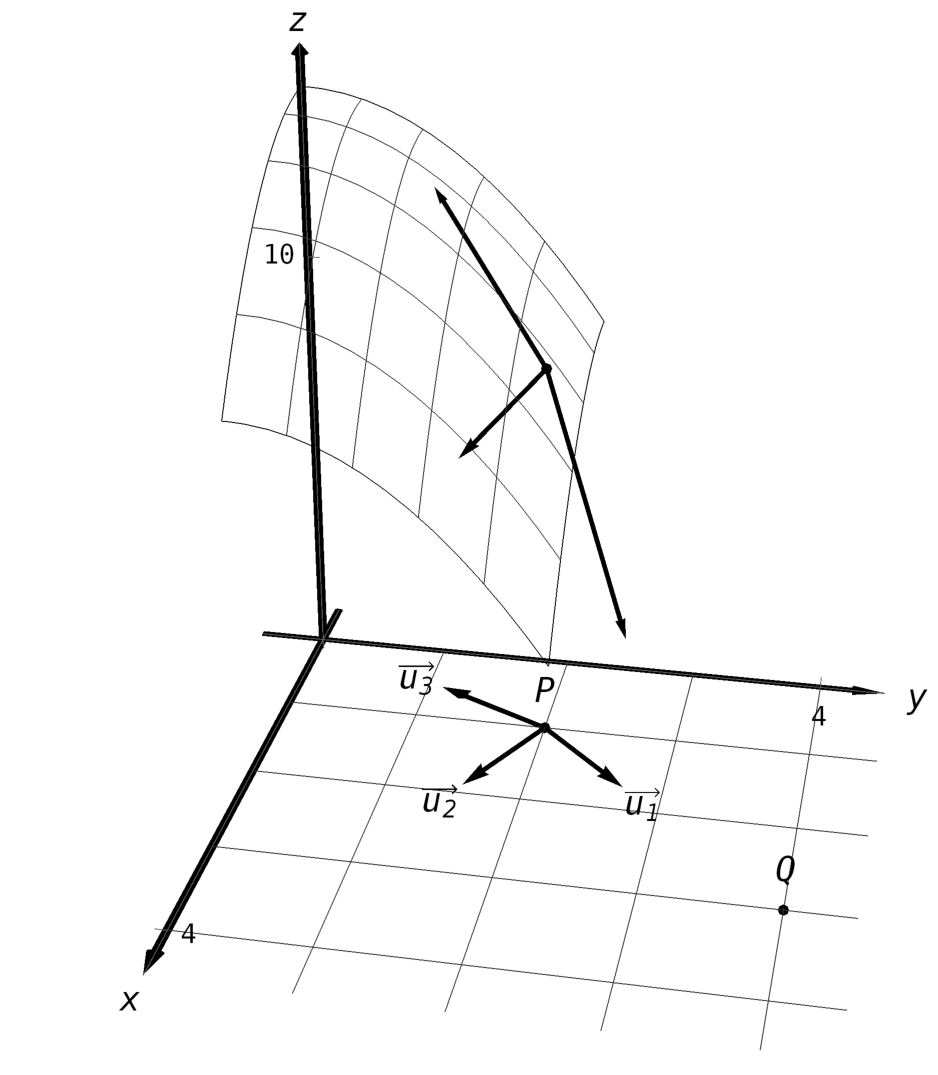
\includegraphics[width=0.4\textwidth]{fig_multi_var_13}
	\caption{Understanding the directional derivative in Example \ref{ex_direct1}.}
	\label{fig_multi_var_13}
	\end{center}
\end{figure}

\xhrulefill{gray}{2.5pt}Solution \xhrulefill{gray}{2.5pt}


We find that $f_x(x,y) = -2x$ and $f_x(1,2) = -2$; $f_y(x,y) = -2y$ and $f_y(1,2) = -4$. 
\begin{enumerate}
	\item Let $\hat u_1$ be the unit vector that points from the point $P=(1,2)$ to the point $Q=(3,4)$, as shown in the figure. The vector $\vv{PQ} = \left( 2,2\right)$; the unit vector in this direction is $\hat u_1=\left( 1/\sqrt{2}, 1/\sqrt{2}\right)$. Thus the directional derivative of $f$ at $(1,2)$ in the direction of $\hat u_1$ is
	$$D_{\hat u_1}f(1,2) = -2\left(\dfrac{1}{\sqrt{2}}\right) +(-4)\left(\dfrac{1}{\sqrt{2}}\right) = -\dfrac{6}{\sqrt{2}}\approx -4.24.$$
	Thus the instantaneous rate of change in moving from the point $(1,2,9)$ on the surface in the direction of $\hat u_1$ (which points toward the point $Q$) is about $-4.24$. Moving in this direction moves one steeply downward.
	
	\item		We seek the directional derivative in the direction of $\left( 2,-1\right)$. The unit vector in this direction is $\hat u_2 = \left( 2/\sqrt{5},-1/\sqrt{5}\right)$. Thus the directional derivative of $f$ at $(1,2)$ in the direction of $\hat u_2$ is
	$$D_{\hat u_2}f(1,2) = -2\left(\dfrac{2}{\sqrt{5}}\right)+(-4)\left(-\dfrac{1}{\sqrt{5}}\right) = 0.$$
	Starting on the surface of $f$ at $(1,2)$ and moving in the direction of $\left( 2,-1\right)$ (or $\hat u_2$) results in no instantaneous change in $z$-value. This is analogous to standing on the side of a hill and choosing a direction to walk that does not change the elevation. One neither walks up nor down, rather just along the side of the hill.
	
	
	\item		At $P=(1,2)$, the direction towards the origin is given by the vector $\left( -1,-2\right)$; the unit vector in this direction is $\hat u_3=\left( -1/\sqrt{5},-2/\sqrt{5}\right)$. The directional derivative of $f$ at $P$ in the direction of the origin is
	$$D_{\hat u_3}f(1,2) = -2\left(-\dfrac{1}{\sqrt{5}}\right) + (-4)\left(-\dfrac{2}{\sqrt{5}}\right) = \dfrac{10}{\sqrt{5}} \approx 4.47.$$
	Moving towards the origin means walking uphill quite steeply, with an initial slope of about $4.47$.
\end{enumerate}
\ifcalculus\vspace{-1cm}\fi
\end{example}

\subsection{The gradient}
	\checkoddpage
\marginpar{\ifoddpage\hspace*{-1.5cm}\else\hspace*{0.25cm}\fi
\includegraphics[width=0.075\textwidth]{youtube}\\
\ifoddpage\hspace*{-1.75cm}\else\hspace*{0.1cm}\fi
\qrcode[height=1.75cm]{https://youtu.be/tIpKfDc295M}
%\includegraphics[width=0.1\textwidth]{gradient}
}

As we study directional derivatives, it will help to make an important connection between the unit vector $\hat u = \left( u_1,u_2\right)$ that describes the direction and the partial derivatives $f_x$ and $f_y$. We start with a definition.

\begin{definition}[Gradient]\label{def:gradient}
Let $z=f(x,y)$ be differentiable on a set $S$ that contains the point $(x_0,y_0)$.
\index{gradient} \index[aut]{gradi\"ent}
\begin{enumerate}
	\item The \textbf{gradient} (\textit{gradi\"ent}) of $f$ is $$\vec{\nabla} f(x,y) = \left( f_x(x,y),f_y(x,y)\right).$$
	\item The \textbf{gradient}  of $f$ at $(x_0,y_0)$ is $$\vec{\nabla} f(x_0,y_0) = \left( f_x(x_0,y_0),f_y(x_0,y_0)\right).$$
\end{enumerate}
\end{definition}

The symbol $\vec{\nabla}$ is named \textbf{nabla}, derived from the Greek name of a Jewish harp. Oddly enough, in mathematics the expression $\vec{\nabla} f$ is pronounced del $f$.

To simplify notation, we often express the gradient as $\vec{\nabla} f = \left( f_x, f_y\right)$. The gradient allows us to compute directional derivatives in terms of a dot product:
\begin{equation}
D_{\hat u\,}f = \vec{\nabla} f\cdot \hat u.
\label{idea:gradient_direct}
\end{equation}

The properties of the dot product studied in Chapter~\ref{chap_vector} allow us to investigate the properties of the directional derivative. Given that the directional derivative gives the instantaneous rate of change of $z$ when moving in the direction of $\hat u$, three questions naturally arise:
\begin{enumerate}
	\item In what direction(s) is the change in $z$ the greatest (i.e., the steepest uphill)?
	\item In what direction(s) is the change in $z$ the least (i.e.,  the steepest downhill)?
	\item In what direction(s) is there no change in $z$?
\end{enumerate}

Relying on the geometric interpretation of the dot product (Theorem~\ref{dotproductgeo}), we have
\begin{equation}\vec{\nabla} f\cdot \hat u = \norm{\vec{\nabla} f}\,\vnorm u \cos(\theta) = \norm{\vec{\nabla} f}\cos(\theta), \label{eq:gradient}\end{equation}
where $\theta$ is the angle between the gradient and $\hat u$. (Since $\hat u$ is a unit vector, $\vnorm{u} = 1$.) This equation allows us to answer the three questions stated previously.

\begin{enumerate}
	\item Equation \eqref{eq:gradient} is maximized when $\cos(\theta) =1$, i.e., when the gradient and $\hat u$ have the same direction. We conclude the gradient points in the direction of greatest $z$ change.
	\item	Equation \eqref{eq:gradient} is minimized when $\cos(\theta) = -1$, i.e., when the gradient and $\hat u$ have opposite directions. We conclude the gradient points in the opposite direction of the least $z$ change.
	\item Equation \eqref{eq:gradient} is 0 when $\cos(\theta) = 0$, i.e., when the gradient and $\hat u$ are orthogonal to each other. We conclude the gradient is orthogonal to directions of no $z$ change. 
\end{enumerate}

This result is rather amazing. Once again imagine standing in a rolling meadow and face the  direction that leads you steepest uphill. Then the direction that leads steepest downhill is directly behind you, and side--stepping either left or right (i.e., moving perpendicularly to the direction you face) does not change your elevation at all.


Recall that a level curve is defined as a curve in the $xy$-plane along which the $z$-values of a function do not change. Let a surface $z=f(x,y)$ be given, and let us represent one such level curve as a vector--valued function, $\vrt = \left( x(t), y(t)\right)$. As the output of $f$ does not change along this curve, $f\big(x(t),y(t)\big) = c$ for all $t$, for some constant $c$.

Since $f$ is constant for all $t$, $\frac{df}{dt} = 0$. By the multivariable chain rule, we also know
\begin{align*}
\frac{df}{dt} &= f_x(x,y)x'(t) + f_y(x,y)y'(t)\\[0.2cm]						
						&= \left( f_x(x,y),f_y(x,y)\right) \cdot \left( x'(t),y'(t)\right)\\[0.2cm]
						&= \vec{\nabla} f \cdot \vrp(t)\\[0.2cm]
						&=0.
\end{align*}

This last equality states $\vec{\nabla} f \cdot \vrp(t) = 0$: the gradient is orthogonal to the derivative of $\vec r$, meaning the gradient is orthogonal to the graph of $\vec r$. Our conclusion: at any point on a surface, the gradient at that point is orthogonal to the level curve that passes through that point.

We restate these ideas in a theorem, then use them in an example.



\begin{theorem}[The gradient and directional derivatives]\label{thm:gradient}
Let $z=f(x,y)$ be differentiable on a set $S$ with gradient $\vec{\nabla} f$, let $P=(x_0,y_0)$ be a point in $S$ and let $\hat u$ be a unit vector.
\begin{enumerate}
	\item The maximum value of $D_{\hat u\,}f(x_0,y_0)$ is $\norm{\vec{\nabla} f(x_0,y_0)}$; the direction of maximal $z$ increase is $\vec{\nabla} f(x_0,y_0)$.
	%obtained when the angle between $\vec{\nabla} f$ and $\hat u$ is 0, i.e.,  the direction of maximal increase is $\vec{\nabla} f$.
	\item   The minimum value of $D_{\hat u\,}f(x_0,y_0)$ is $-\norm{\vec{\nabla} f(x_0,y_0)}$; the direction of maximal $z$ decrease is $-\vec{\nabla} f(x_0,y_0)$.
	%The minimum value of $D_{\hat u\,}f$ is $-\norm{\vec{\nabla} f}$, obtained when the angle between $\vec{\nabla} f$ and $\hat u$ is $\pi$, i.e., the direction of minimal increase is $-\vec{\nabla} f$.
	\item At $P$, $\vec{\nabla} f(x_0,y_0)$ is orthogonal to the level curve passing through $\big(x_0,y_0,f(x_0,y_0)\big)$.
	%$D_{\hat u\,}f = 0$ when $\vec{\nabla} f$ and $\hat u$ are orthogonal.
	\index{gradient}\index{directional derivative}\index{derivative!directional}\index{level curves}\index{gradient!and level curves}\index[aut]{gradi\"ent}\index[aut]{richtingsafgeleide}
\end{enumerate}
\end{theorem}

We now illustrate how to find the directions of  maximal increase and decrease. 

\begin{example}\label{ex_direct2}
Let $f(x,y) = \sin(x)\cos(y)$ and let $P=(\pi/3,\pi/3)$. Find the directions of maximal increase and decrease, and find a direction where the instantaneous rate of $z$ change is 0.

\xhrulefill{gray}{2.5pt}Solution \xhrulefill{gray}{2.5pt}

We begin by finding the gradient. We have that $f_x = \cos (x)\cos(y)$ and $f_y = -\sin(x)\sin(y)$, thus 
$$\vec{\nabla} f = \left( \cos(x)\cos(y),-\sin(x)\sin(y)\right)$$
and, at $P$
$$ \vec{\nabla} f\left(\frac{\pi}3,\frac{\pi}3\right) = \left(\frac14,-\frac34\right).$$
Thus the direction of maximal increase is $\left( 1/4, -3/4\right)$. In this direction, the instantaneous rate of $z$ change is $||\left( 1/4,-3/4\right)|| = \sqrt{10}/4 \approx 0.79.$ 

Figure \ref{fig_multi_var_14} shows the surface. The gradient is drawn at $P$ with a dashed line (because of the nature of this surface, the gradient points into the surface). Let $\hat u = \left( u_1, u_2\right) $ be the unit vector in the direction of $\vec{\nabla} f$ at $P$. The graph also contains the vector $\left( u_1, u_2, ||\vec{\nabla} f\,||\right)$. This vector has a run of 1 (because in the $xy$-plane it moves 1 unit) and a rise of $||\vec{\nabla} f\,||$, hence we can think of it as a vector with slope of $||\vec{\nabla} f\,||$ in the direction of $\vec{\nabla} f$, helping us visualize how steep the surface is in its steepest direction. 


\begin{figure}[H]
	\begin{center}
			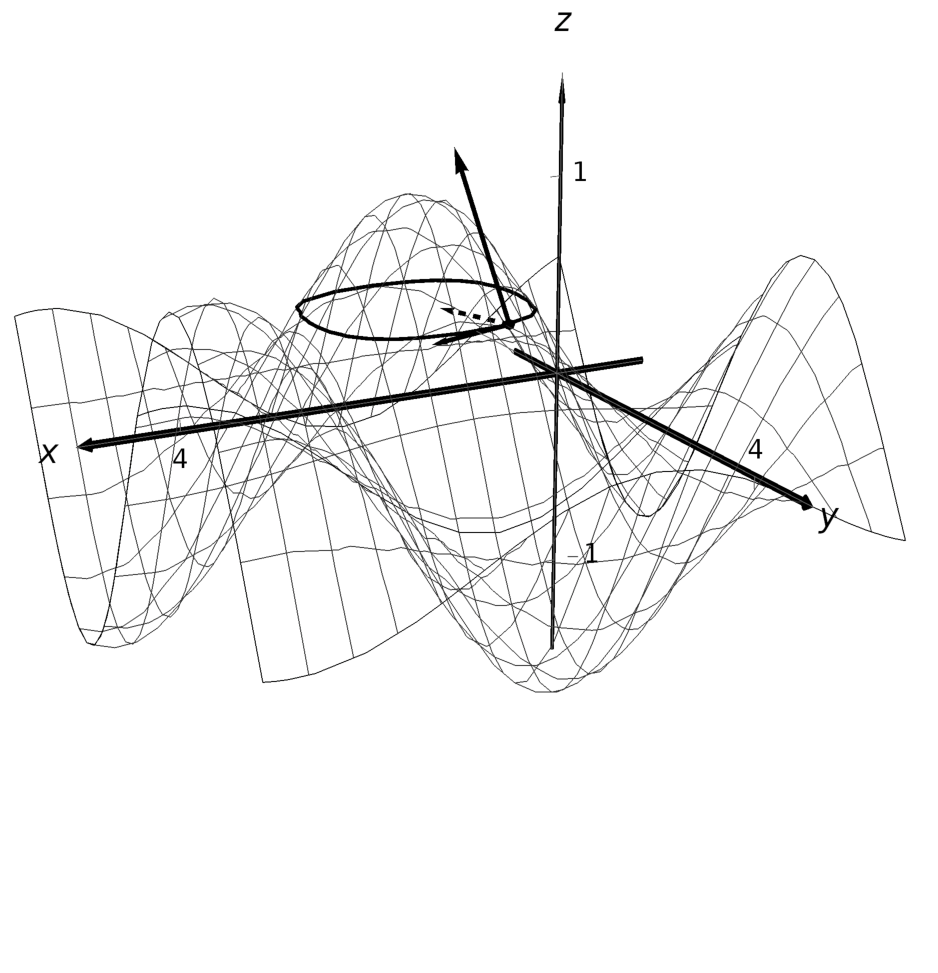
\includegraphics[width=0.5\textwidth]{fig_multi_var_14}
	\caption{Graphing the surface and important directions in Example \ref{ex_direct2}.}
	\label{fig_multi_var_14}
	\end{center}
\end{figure}



The direction of maximal decrease is $\left( -1/4,3/4\right)$; in this direction the instantaneous rate of $z$ change is $-\sqrt{10}/4 \approx -0.79$.

Any direction orthogonal to $\vec{\nabla} f$ is a direction of no $z$ change. We have two choices: the direction of $\left( 3,1\right)$ and the direction of $\left( -3,-1\right)$. The unit vector in the direction of $\left( 3,1\right)$ is shown in the graph as well. The level curve at $z=\sqrt{3}/4$ is drawn: recall that along this curve the $z$-values do not change. Since $\left( 3,1\right)$ is a direction of no $z$-change, this vector is tangent to the level curve at $P$.
\end{example}

It is as well important to figure out when $\vec{\nabla} f=0$. 

\begin{example}\label{ex_direct9}
Let $f(x,y) = -x^2+2x-y^2+2y+1$. Find the directional derivative of $f$ in any direction at $P=(1,1)$.

\xhrulefill{gray}{2.5pt}Solution \xhrulefill{gray}{2.5pt}

We find $\vec{\nabla} f = \left( -2x+2, -2y+2\right)$. At $P$, we have $\vec{\nabla} f(1,1) = \left(0,0\right)$. 
According to Theorem \ref{thm:gradient}, this is the direction of maximal increase. However, $\left( 0,0\right)$ is directionless; it has no displacement. And regardless of the unit vector $\hat u$ chosen, $D_{\hat u\,}f = 0$.

Figure \ref{fig_multi_var_15} helps us understand what this means. We can see that $P$ lies at the top of a paraboloid. In all directions, the instantaneous rate of change is 0. So what is the direction of maximal increase? It is fine to give an answer of $\vec 0 = \left( 0,0\right)$, as this indicates that all directional derivatives are 0.

\begin{figure}[H]
	\begin{center}
			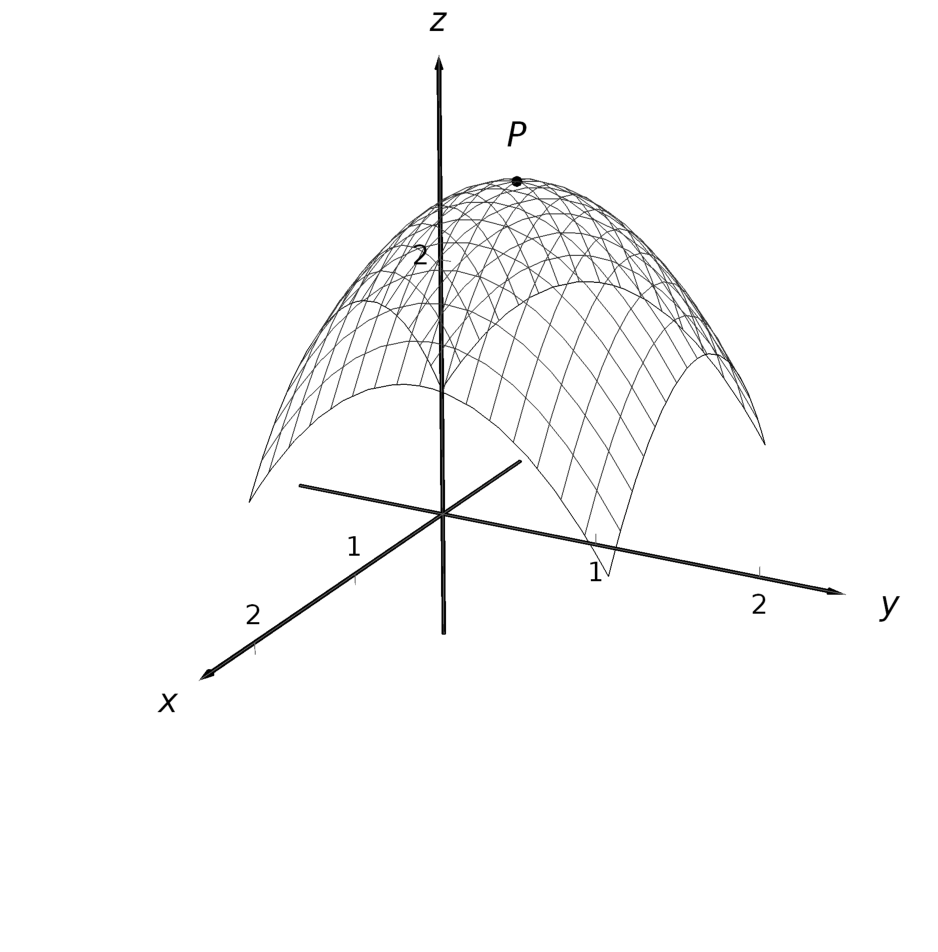
\includegraphics[width=0.5\textwidth]{fig_multi_var_15}
	\caption{At the top of a paraboloid, all directional derivatives are 0.}
	\label{fig_multi_var_15}
	\end{center}
\end{figure}


\end{example}

\ifmathematica
In Mathematica, we could have computed the gradient in Example~\ref{ex_direct9} using the command \lstinline{Grad} as follows \index{\lstinline{Grad}}\index[aut]{\lstinline{Grad}}
	\begin{mdframed}[default,backgroundcolor=gray!40,roundcorner=8pt]
\begin{mmaCell}[morefunctionlocal={x,y}]{Input}
  Grad[-x^2 + 2*x - y^2 + 2*y + 1, \{x, y\}]
\end{mmaCell}

\begin{mmaCell}{Output}
  \{2-2 x,2-2 y\}
\end{mmaCell}
\end{mdframed}
\fi

\ifpython
In Mathematica, we could have computed the gradient in Example~\ref{ex_direct9} using the command \lstinline{diff} as follows
\begin{pyin}
from sympy import symbols, diff
x, y = symbols('x y')
f = -x**2+2*x-y**2+2*y+1
(diff(f, x), diff(f, y))
\end{pyin}
\begin{pyout}
(2 - 2*x, 2 - 2*y)
\end{pyout}
\fi

The fact that the gradient of a surface always points in the direction of steepest increase/decrease is very useful, as illustrated in the following example.

\begin{example}\label{ex_direct3}
Consider the surface given by $f(x,y)= 20-x^2-2y^2$. Water is poured on the surface at $(1,1/4)$. What path does it take as it flows downhill?

\xhrulefill{gray}{2.5pt}Solution \xhrulefill{gray}{2.5pt}

Let $\vrt = \left( x(t), y(t)\right)$ be the vector--valued function describing the path of the water in the $xy$-plane; we seek $x(t)$ and $y(t)$. We know that water will always flow downhill in the steepest direction; therefore, at any point on its path, it will be moving in the direction of $-\vec{\nabla} f$. We ignore the physical effects of momentum on the water. Thus $\vrp(t)$ will be parallel to $\vec{\nabla} f$, and there is some constant $c$ such that $c\vec{\nabla} f = \vrp(t) = \left( x'(t), y'(t)\right)$. 

We find $\vec{\nabla} f = \left( -2x, -4y\right)$ and write $x'(t)$ as $\frac{dx}{dt}$ and $y'(t)$ as $\frac{dy}{dt}$. Then 
\begin{align*}
c\vec{\nabla} f &= \left( x'(t), y'(t)\right) \\
\Leftrightarrow \qquad \left( -2cx, -4cy \right) & = \left( \frac{dx}{dt}, \frac{dy}{dt}\right).
\end{align*}
This implies
$$-2cx = \frac{dx}{dt} \qquad \text{and} \qquad  -4cy =\frac{dy}{dt},$$
i.e.\
$$c = -\frac{1}{2x}\frac{dx}{dt} \qquad \text{and} \qquad  c =-\frac{1}{4y}\frac{dy}{dt}.$$
As $c$ equals both expressions, we have
%\drawexampleline%
$$\frac{1}{2x}\frac{dx}{dt} =\frac{1}{4y}\frac{dy}{dt}.$$
To find an explicit relationship between $x$ and $y$, we can integrate both sides with respect to $t$. Recall from our study of differentials that $\ds \frac{dx}{dt}dt = dx$. Thus:
\begin{align*}
\int \frac{1}{2x}\frac{dx}{dt}\ dt &=\int \frac{1}{4y}\frac{dy}{dt}\ dt \\
\Leftrightarrow \qquad \int \frac{1}{2x}\ dx &=\int\frac{1}{4y}\ dy \\
\Leftrightarrow \qquad \qquad \frac 12\ln|x| &= \frac14\ln|y| +C_1\\
\Leftrightarrow \qquad \qquad 2\ln|x| &= \ln|y| +4C_1\\
\Leftrightarrow \qquad \qquad \ln (x^2) &= \ln|y|+4C_1.% &= y,
\intertext{Now raise both sides as a power of $e$:}
%\end{align*}
%where we skip some algebra in the last step. 
%\begin{align*}
x^2 & = e^{\ln |y|+4C_1}\\
  \qquad \Leftrightarrow \qquad x^2 & = e^{\ln |y|}e^{4C_1}.\\
 \intertext{From which it follows that}
 x^2 & = yC_2,\\
 \intertext{where  $C_2=\pm e^{4C_1}$, or alternatively}
 Cx^2 &= y,
\end{align*}
where $C=1/C_2$. As the water started at the point $(1,1/4)$, we can solve for $C$:
$$C(1)^2 = \frac14 \quad \Leftrightarrow \quad C = \frac14.$$

Thus the water follows the curve $y=x^2/4$ in the $xy$-plane. The surface and the path of the water is graphed in Figure \ref{fig_multi_var_16a}. In Figure~\ref{fig_multi_var_16b}, the level curves of the surface are plotted in the $xy$-plane, along with the curve $y=x^2/4$. Notice how the path intersects the level curves at right angles. As the path follows the gradient downhill, this reinforces the fact that the gradient is orthogonal to level curves.


\begin{figure}[H]
\centering
%\raisebox{0.5cm}{
\subfigure[\label{fig_multi_var_16a}]{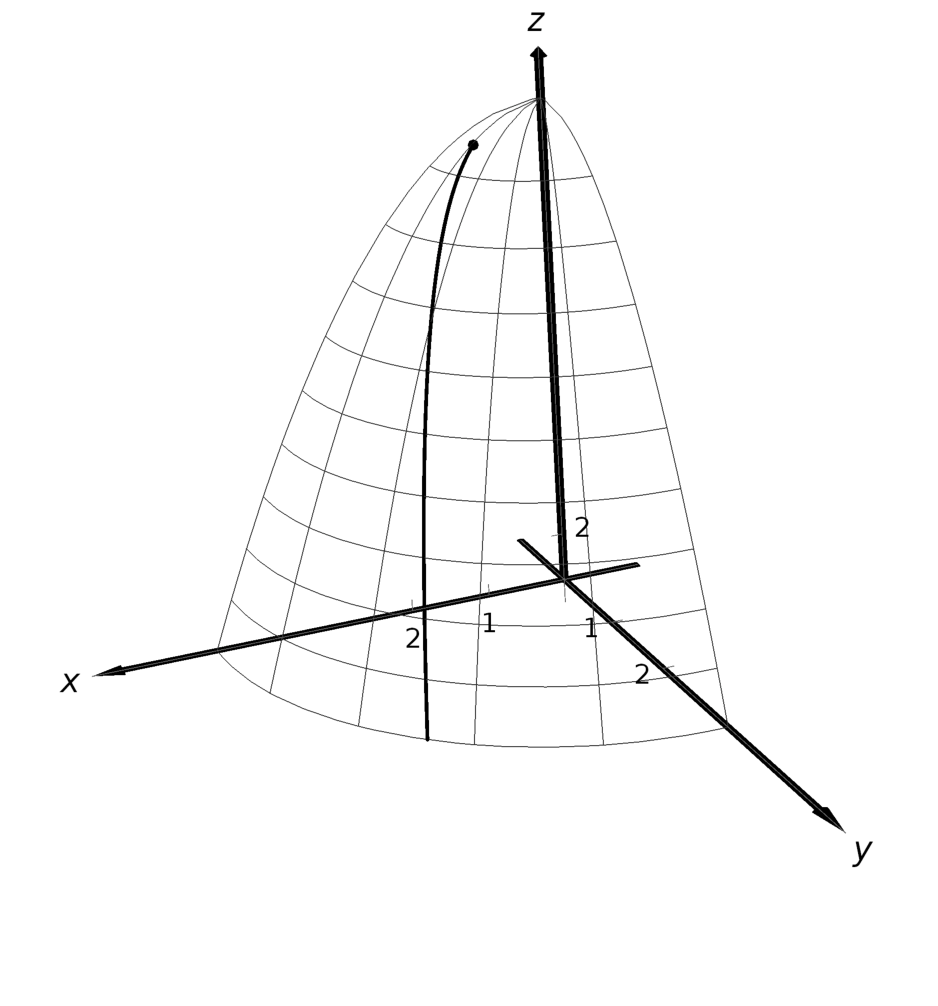
\includegraphics[width=0.43\textwidth]{fig_multi_var_16a}}
\qquad
\subfigure[\label{fig_multi_var_16b}]{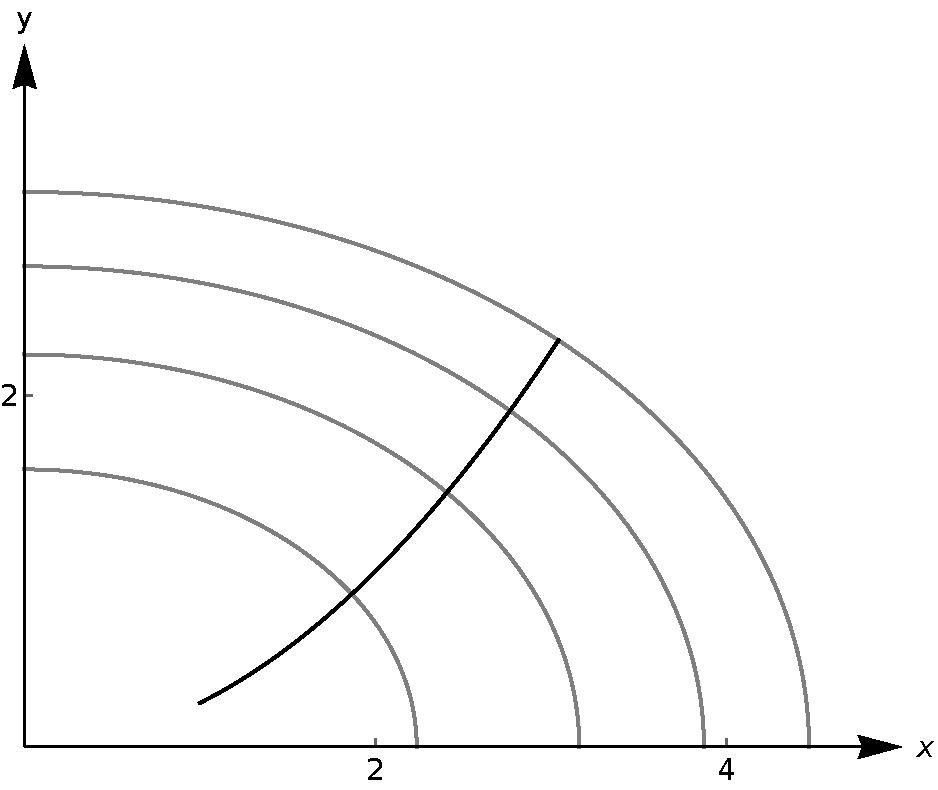
\includegraphics[width=0.43\textwidth]{fig_multi_var_16b} }
\caption{A graph of the surface described in Example \ref{ex_direct3} along with the path in the $xy$-plane with the level curves.}
\end{figure}

\end{example}


\ifcalculus
\subsection{Functions of three variables}
The concepts of directional derivatives and the gradient are easily extended to three (and more) variables. We combine the concepts behind Definitions \ref{def:direct_deriv} and \ref{def:gradient} and Theorem \ref{thm:direct_deriv1} into one set of definitions.

\begin{definition}[Directional derivatives and gradient with three variables]\label{def:direct_deriv3}
Let $w=f(x,y,z)$ be differentiable on a set $D$ and let $\hat u $ be a unit vector in $\mathbb{R}^3$.\index{gradient}\index{directional derivative}\index{derivative!directional}\index[aut]{gradi\"ent}\index[aut]{richtingsafgeleide}
\begin{enumerate}
	\item	The \textbf{gradient of $f$} is $\vec{\nabla} f = \left(f_x,f_y,f_z\right)$.
	\item The \textbf{directional derivative of $f$ in the direction of $\hat u$} is $$D_{\hat u\,}f=\vec{\nabla} f\cdot \hat u.$$
\end{enumerate}
\end{definition}

The same properties of the gradient given in Theorem \ref{thm:gradient}, when $f$ is a function of two variables, hold for $f$, a function of three variables.

\begin{theorem}[The gradient and directional derivatives with three variables]\label{thm:gradient3}
Let $w=f(x,y,z)$ be differentiable on a set $D$, let $\vec{\nabla} f$ be the gradient of $f$, and let $\hat u$ be a unit vector.\index{gradient}\index{directional derivative}\index{derivative!directional}\index[aut]{gradi\"ent}\index[aut]{richtingsafgeleide}
\begin{enumerate}
	\item The maximum value of $D_{\hat u\,}f$ is $\norm{\vec{\nabla} f}$, obtained when the angle between $\vec{\nabla} f$ and $\hat u$ is 0, i.e.,  the direction of maximal increase is $\vec{\nabla} f$.
	\item The minimum value of $D_{\hat u\,}f$ is $-\norm{\vec{\nabla} f}$, obtained when the angle between $\vec{\nabla} f$ and $\hat u$ is $\pi$, i.e., the direction of maximal decrease is $-\vec{\nabla} f$.
	\item $D_{\hat u\,}f = 0$ when $\vec{\nabla} f$ and $\hat u$ are orthogonal.
\end{enumerate}
\end{theorem}

We interpret the third statement of the theorem as the gradient is orthogonal to level surfaces, the three--variable analogue to level curves.

\fi

\ifanalysis
\subsection{Functions of $n$ variables}

The concepts of directional derivatives and the gradient are easily extended to $n$ variables. We combine the concepts behind Definitions \ref{def:direct_deriv} and \ref{def:gradient} and Theorem \ref{thm:direct_deriv1} into one set of definitions.


\begin{definition}[Directional derivatives and gradient with $n$ variables]\label{def:direct_deriv3}

Let $w=f(\mathbf{x})$ be differentiable on a set $D$ and let $\hat u $ be a unit vector in $\mathbb{R}^n$.\index{gradient}\index{directional derivative}\index{derivative!directional}\index[aut]{gradi\"ent}\index[aut]{richtingsafgeleide}
\begin{enumerate}
	\item	The \textbf{gradient of $f$} is $\vec{\nabla} f = \mathbf{f_x}=\left( f_{x_1},f_{x_2},\ldots,f_{x_n}\right)$.
	\item The \textbf{directional derivative of $f$ in the direction of $\hat u$} is $$D_{\hat u\,}f=\vec{\nabla} f\cdot \hat u.$$
\end{enumerate}

\end{definition}

The same properties of the gradient given in Theorem \ref{thm:gradient}, hold for a function of three variables.

\begin{theorem}[The gradient and directional derivatives with $n$ variables]\label{thm:gradient3}

Let $w=f(\mathbf{x})$ be differentiable on a set $D$, let $\vec{\nabla} f$ be the gradient of $f$, and let $\hat u$ be a unit vector.\index{gradient}\index{directional derivative}\index{derivative!directional}\index[aut]{gradi\"ent}\index[aut]{richtingsafgeleide}
\begin{enumerate}
	\item The maximum value of $D_{\hat u\,}f$ is $\norm{\vec{\nabla} f}$, obtained when the angle between $\vec{\nabla} f$ and $\hat u$ is 0, i.e.,  the direction of maximal increase is $\vec{\nabla} f$.
	\item The minimum value of $D_{\hat u\,}f$ is $-\norm{\vec{\nabla} f}$, obtained when the angle between $\vec{\nabla} f$ and $\hat u$ is $\pi$, i.e., the direction of maximal decrease is $-\vec{\nabla} f$.
	\item $D_{\hat u\,}f = 0$ when $\vec{\nabla} f$ and $\hat u$ are orthogonal.
\end{enumerate}

\end{theorem}

We interpret the third statement of the theorem as the gradient is orthogonal to level surfaces, the three--variable analogue to level curves.



\fi

\begin{example}\label{ex_direct5}
If a point source $S$ is radiating energy, the intensity $I$ at a given point $P$ in space is inversely proportional to the square of the distance between $S$ and $P$. That is, when $S=(0,0,0)$, it holds that \linebreak $$\ds I(x,y,z) = \frac{k}{x^2+y^2+z^2}$$ for some constant $k$.

Let $k=1$, let $\hat u = \left( 2/3, 2/3, 1/3\right)$ be a unit vector, and let $P = (2,5,3).$ Measure distances in centimetres. Find the directional derivative of $I$ at $P$ in the direction of $\hat u$, and find the direction of greatest intensity increase at $P$.

\xhrulefill{gray}{2.5pt}Solution \xhrulefill{gray}{2.5pt}

We need the gradient $\vec{\nabla} I$, so we compute $I_x$, $I_y$ and $I_z$:
$$\begin{array}{rrl}
&\vec{\nabla} I &= \left( \dfrac{-2x}{(x^2+y^2+z^2)^2},\dfrac{-2y}{(x^2+y^2+z^2)^2},\dfrac{-2z}{(x^2+y^2+z^2)^2}\right)\\[0.2cm]
\Rightarrow &\vec{\nabla} I(2,5,3) &= \left( \dfrac{-4}{1444},\dfrac{-10}{1444},\dfrac{-6}{1444}\right) \approx \left( -0.003,-0.007,-0.004\right)\\[0.2cm]
\Rightarrow &D_{\hat u\,}I &= \vec{\nabla} I(2,5,3)\cdot \hat u\\[0.2cm]
&					&= -\dfrac{17}{2166} \approx -0.0078.\\[0.2cm]
\end{array}$$
The directional derivative tells us that moving in the direction of $\hat u$ from $P$ results in a decrease in intensity of about $-0.008$ units per centimetre. The intensity is decreasing as $\hat u$ moves one farther from the origin than $P$.

The gradient gives the direction of greatest intensity increase. Notice that 
\begin{align*}
\vec{\nabla} I(2,5,3) &= \left( \frac{-4}{1444},\frac{-10}{1444},\frac{-6}{1444}\right)\\
			&= \frac{2}{1444}\left(-2,-5,-3\right).
\end{align*}
That is, the gradient at $(2,5,3)$ is pointing in the direction of $\left( -2,-5,-3\right)$, that is, towards the origin. That should make intuitive sense: the greatest increase in intensity is found by moving towards to source of the energy.
\end{example}

The directional derivative allows us to find the instantaneous rate of $z$ change in any direction at a point. We can use these instantaneous rates of change to define lines and planes that are tangent to a surface at a point, which is the topic of the next section.

\ifanalysis


  Using the gradient of functions of $n$ variables introduced in Definition~\ref{def:direct_deriv3}, we can easily state the multivariable counterpart of the mean value theorem of differentiation (Theorem~\ref{thm:mvt}). 
\pagebreak
  \begin{theorem}[Mean value theorem for functions of $n$ variables]\label{thm:mvtmulti}

Let $f$ be differentiable on $D$, let $\vec{a}$ and $\vec{b}$ belong to $D$ and let $\vec{\nabla} f$ be the gradient of $f$, then there exists a point $\vec{c}$ on the line segment $L$ connecting $\vec{a}$ and $\vec{b}$ for which it holds that
$$
\vec{\nabla} f(\vec{c})\cdot\left(\vec{b}-\vec{a}\right)=f(\vec{b})-f(\vec{a})\,.
$$

\end{theorem}

\begin{proof}
The key of the proof of this theorem is to design an appropriate function of one variable to which we can then apply the mean value theorem for functions of one variable (Theorem~\ref{thm:mvt}). For that purpose, we ought to realize that as we let $t$ range from 0 to 1, $\vec{a}+t(\vec{b}-\vec{a})$ traces out the line segment $L$.   So, the idea of the proof is to apply the one-variable mean-value theorem to the function
$$
\vec{\phi}(t) =\vec{a}+t\left(\vec{b}-\vec{a}\right)=(1-t)\vec{a}+t\vec{b}\,,
$$
for $t\in[0,1]$. Clearly, $\vec{\phi}(t)$ is differentiable with $\vec{\phi}'(t)=\vec{b}-\vec{a}$. Consequently, the composition $g=f\circ\,\vec{\phi}$ is differentiable  by the chain rule. Since $g$ provides a mapping from the unit interval to the real numbers, i.e. $g:[0,1]\mapsto\mathbb{R}$, the mean value theorem for functions of one variable applied to $g$ gives us a point $\xi$ in $[0,1]$, such that
$$
g(1)-g(0)=g'(\xi)\,.
$$
Now, let $\mathbf{c}=\vec{\phi}(\xi)\in\,L$. We then have
\begin{eqnarray*}
f(\vec{b})-f(\vec{a})&=&g(1)-g(0)\\
&=&g'(\xi)\,,\\
&=&\vec{\nabla}\,f\left(\vec{\phi}(\xi)\right)\cdot\vec{\phi}'(\xi)\,\\
&=&\vec{\nabla}\,f(\vec{c})\cdot(\vec{b}-\vec{a})\,,
\end{eqnarray*}
which concludes the proof. 
\end{proof}
For comprehensiveness, it should be noted that the transition from $g'(\xi)$ to $\vec{\nabla}\,f\left(\vec{\phi}(\xi)\right)\cdot\vec{\phi}'(\xi)$ in the right-hand side follows from clever use of the chain rule. More precisely, $f$ is a function of $n$ variables $x_i$ applied to the output of the single-variable vector-valued function $\vec{\phi}(t)$ with components $x_i=\phi_i(t)$, so the chain rule (Theorem~\ref{thm:multi_chain}) immediately gives
$$
\dfrac{dg}{dt}=\dfrac{\partial f}{\partial x_1}\dfrac{dx_1}{dt}+\dfrac{\partial f}{\partial x_2}\dfrac{dx_2}{dt}+\cdots+\dfrac{\partial f}{\partial x_n}\dfrac{dx_n}{dt}\,,
$$
which can be written using the dot product as
$$
\dfrac{dg}{dt}=\left(\dfrac{\partial f}{\partial x_1},\dfrac{\partial f}{\partial x_2},\ldots,\dfrac{\partial f}{\partial x_n}\right)\cdot\left(\dfrac{dx_1}{dt},\dfrac{dx_2}{dt},\ldots,\dfrac{dx_n}{dt}\right)\,.
$$


%https://books.google.be/books?id=HxHjBQAAQBAJ&pg=PA85&lpg=PA85&dq=mean+value+theorem+proof+several+variables&source=bl&ots=DT7tunuIUi&sig=ACfU3U0kZGq-Qh1aIvdyxo79ZnGhjKcqxw&hl=nl&sa=X&ved=2ahUKEwiDy87U_pDhAhUjSRUIHdo7Asc4ChDoATAJegQICRAB#v=onepage&q=mean%20value%20theorem%20proof%20several%20variables&f=false


\fi

\section{Tangent lines, normal lines, and tangent planes}\label{sec:multi_tangent}

\subsection{Tangent and normal lines}
Derivatives and tangent lines go hand--in--hand. Given $y=f(x)$, the line tangent to the graph of $f$ at $x=x_0$ is the line through $\big(x_0,f(x_0)\big) $ with slope $\fp(x_0)$; that is, the slope of the tangent line is the instantaneous rate of change of $f$ at $x_0$. When dealing with functions of two variables, the graph is no longer a curve but a surface. At a given point on the surface, it seems there are many lines that fit our intuition of being tangent to the surface. 

In Figure \ref{fig_multi_var_17} we see lines that are tangent to curves in space. Since each curve lies on a  surface, it makes sense to say that the lines are also tangent to the surface. The next definition formally defines what it means to be tangent to a surface. %Recall that to write the equation of a line we need a point and a direction. 

\begin{figure}[H]
	\begin{center}
			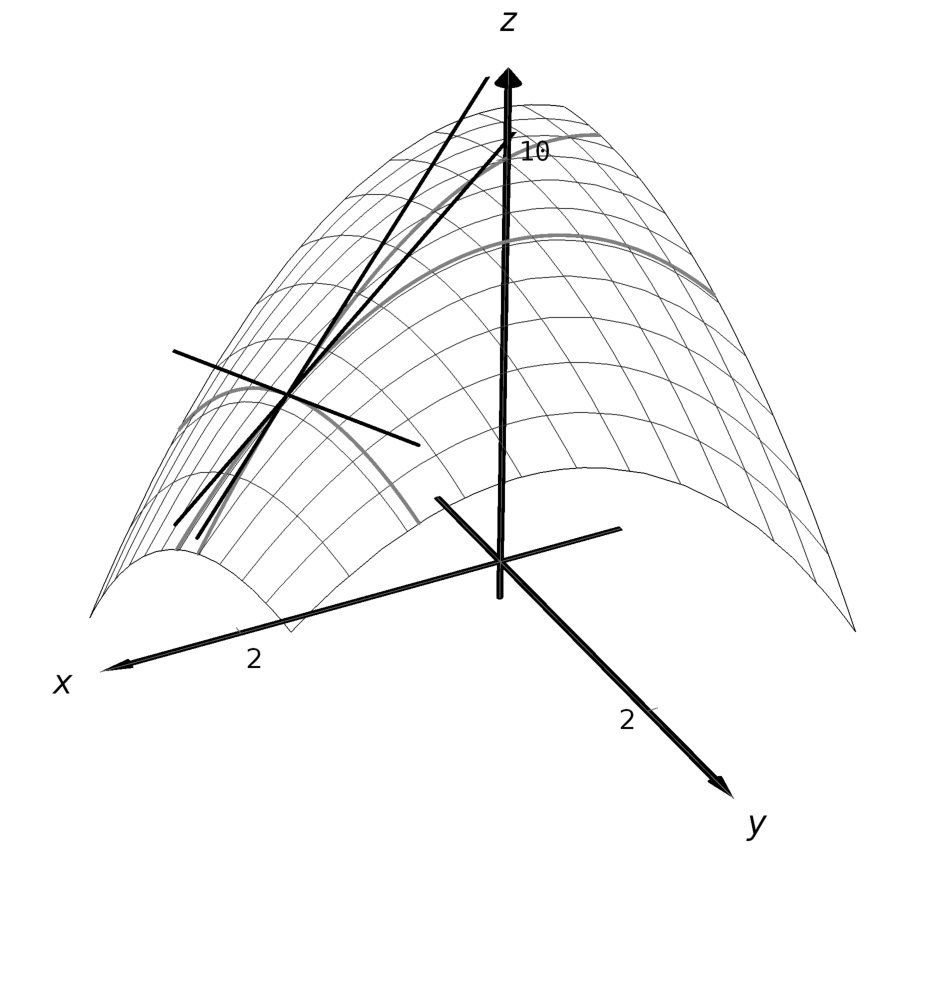
\includegraphics[width=0.5\textwidth]{fig_multi_var_17}
	\caption{Showing various lines tangent to a surface.}
	\label{fig_multi_var_17}
	\end{center}
\end{figure}






\begin{definition}[Directional tangent line]\label{def:directional_tangent_line}
Let $z=f(x,y)$ be differentiable on a set $S$ containing $(x_0,y_0)$ and let $\hat u = \left( u_1, u_2\right)$ be a unit vector.
\index{tangent line!directional} \index[aut]{raaklijn}
\vspace{-0.5cm}
\begin{enumerate}
	\item The line $\ell_x$ through $\big(x_0,y_0,f(x_0,y_0)\big)$ parallel to $\left( 1,0,f_x(x_0,y_0)\right)$	is \textbf{the tangent line to $f$ in the direction of $x$ at $(x_0,y_0)$}.
	
	\item The line $\ell_y$  through $\big(x_0,y_0,f(x_0,y_0)\big)$ parallel to $\left( 0,1,f_y(x_0,y_0)\right)$ is \textbf{the tangent line to $f$ in the direction of $y$ at $(x_0,y_0)$}.
	
	\item	 The line $\ell_{\hat u}$ through $\big(x_0,y_0,f(x_0,y_0)\big)$ parallel to $\left( u_1,u_2,D_{\hat u\,}f(x_0,y_0)\right)$ is \textbf{the tangent line to $f$ in the direction of $\hat u$ at $(x_0,y_0)$}.
	\end{enumerate}
\end{definition}


It is instructive to consider each of three directions given in the definition in terms of slope. The direction of $\ell_x$ is $\left( 1,0,f_x(x_0,y_0)\right)$; that is, the ``run'' is one unit in the $x$-direction and the rise is $f_x(x_0,y_0)$ units in the $z$-direction. Note how the slope is just the partial derivative with respect to $x$. A similar statement can be made for $\ell_y$. The direction of $\ell_{\hat u}$ is $\left( u_1,u_2,D_{\hat u\,}f(x_0,y_0)\right)$; the run is one unit in the $\hat u$ direction (where $\hat u$ is a unit vector) and the rise is the directional derivative of $z$ in that direction.


Definition \ref{def:directional_tangent_line} leads to the following parametric equations of directional tangent lines:


$$\ell_x(t) = \left\{\begin{array}{rcl} x&=&x_0+t \\ y&=&y_0\\z&=&z_0+f_x(x_0,y_0)t, \end{array}\right. \, \ell_y(t)=\left\{\begin{array}{rcl} x&=&x_0 \\ y&=&y_0+t\\z&=&z_0+f_y(x_0,y_0)t \end{array}\right.\  \text{and}\, \ell_{\hat u}(t)=\left\{\begin{array}{rcl} x&=&x_0+u_1t \\ y&=&y_0+u_2t\\z&=&z_0+D_{\hat u\,}f(x_0,y_0)t. \end{array}\right.$$
where $z_0=f(x_0,y_0)$.

\begin{example}\label{ex_tpl1}
Find the lines tangent to the surface $z=\sin (x)\cos(y)$ at $(\pi/2,\pi/2)$ in the $x$- and $y$- directions and also in the direction of $\vec v = \left( -1,1\right).$

\xhrulefill{gray}{2.5pt}Solution \xhrulefill{gray}{2.5pt}

The partial derivatives with respect to $x$ and $y$ are:
\begin{align*}
f_x(x,y) &= \cos(x)\cos(y)\\
f_y(x,y) &= -\sin(x)\sin(y) .
\end{align*}
from which it follows that $f_x(\pi/2,\pi/2) = 0$ and $f_y(\pi/2,\pi/2)=-1$. At $(\pi/2,\pi/2)$, the $z$-value is 0.

Thus the parametric equations of the line tangent to $f$ at $(\pi/2,\pi/2)$ in the directions of $x$  and $y$ are:
$$\ell_x(t) = \left\{\begin{array}{l} x=\pi/2 + t\\ y=\pi/2 \\z=0 \end{array}\right. \quad \text{and}\quad 
\ell_y(t) = \left\{\begin{array}{l} x=\pi/2 \\ y=\pi/2+t \\z=-t. \end{array}\right.$$
The two lines are shown with the surface in Figure \ref{fig_multi_var_18a}.

\begin{figure}[H]
\centering
%\raisebox{0.5cm}{
\subfigure[\label{fig_multi_var_18a}]{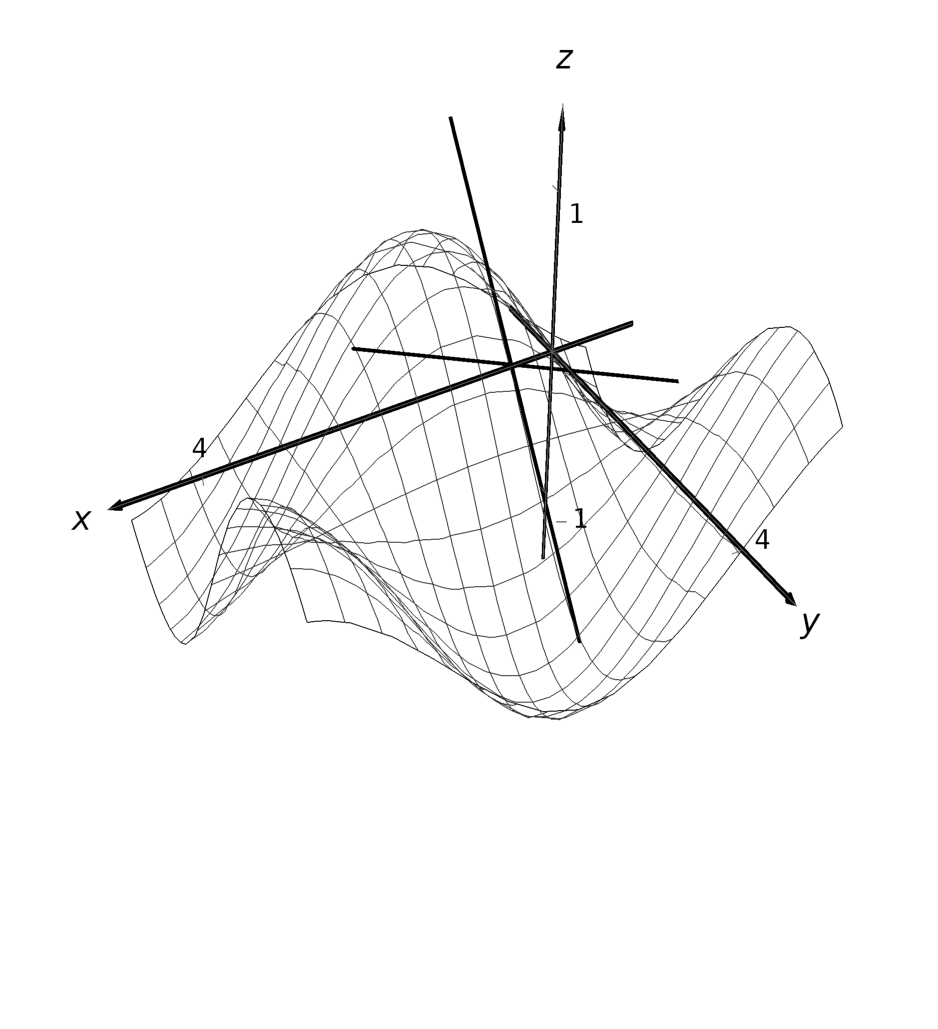
\includegraphics[width=0.43\textwidth]{fig_multi_var_18a}}
\qquad
\subfigure[\label{fig_multi_var_18b}]{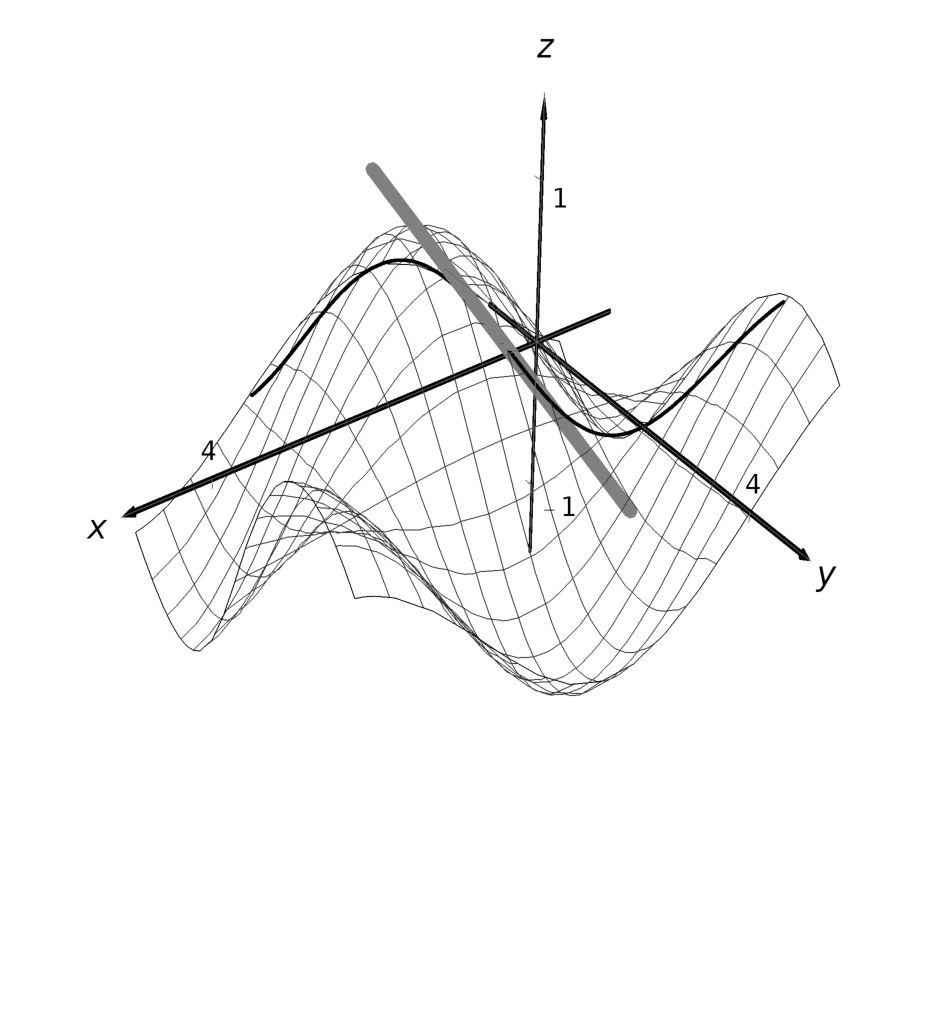
\includegraphics[width=0.43\textwidth]{fig_multi_var_18b}}
\caption{A surface and directional tangent lines in Example \ref{ex_tpl1}.}
\end{figure}

To find the equation of the tangent line in the direction of $\vec v$, we first find the unit vector in the direction of $\vec v$: $\hat u = \left( -1/\sqrt{2},1/\sqrt{2}\right)$. The directional derivative at $(\pi/2,\pi/2)$ in the direction of $\hat u$ is 
$$D_{\hat u\,}f\left(\dfrac{\pi}{2},\dfrac{\pi}{2}\right) = \left( 0,-1\right) \cdot \left( -\dfrac{1}{\sqrt{2}},\dfrac{1}{\sqrt{2}}\right) = -\dfrac{1}{\sqrt{2}}.$$
Thus the directional tangent line is 
$$\ell_{\hat u}(t) = \left\{\begin{array}{l} x= \dfrac{\pi}{2} -\dfrac{t}{\sqrt{2}}\\ y = \dfrac{\pi}{2} + \dfrac{t}{\sqrt{2}} \\ z= -\dfrac{t}{\sqrt{2}}\end{array}\right. .$$
The curve through $(\pi/2,\pi/2,0)$ in the direction of $\vec v$ is shown in Figure \ref{fig_multi_var_18b} along with $\ell_{\hat u}(t)$.



\end{example}


The following example shows that the points on surfaces where all tangent lines have a slope of 0 can give us some information about the extrema of functions of several variables. 

\begin{example}\label{ex_tpl2}
Let $f(x,y) = 4xy-x^4-y^4$. Find the equations of all directional tangent lines to $f$ at $(1,1)$.

\xhrulefill{gray}{2.5pt}Solution \xhrulefill{gray}{2.5pt}

First note that $f(1,1) = 2$. We need to compute directional derivatives, so we need $\vec{\nabla} f$. We begin by computing partial derivatives.
$$f_x = 4y-4x^3 \quad \Rightarrow \quad f_x(1,1) = 0;\qquad f_y = 4x-4y^3 \quad \Rightarrow \quad f_y(1,1) = 0.$$
Thus $\vec{\nabla} f(1,1) = \left( 0,0\right)$. Let $\hat u = \left( u_1,u_2\right)$ be any unit vector. The directional derivative of $f$ at $(1,1)$ will be $D_{\hat u\,}f(1,1) = \left( 0,0\right)\cdot \left( u_1,u_2\right) = 0$. It does not matter what direction we choose; the directional derivative is always 0. Therefore
$$\ell_{\hat u}(t) = \left\{\begin{array}{l} x= 1 +u_1t\\ y = 1+ u_2 t\\ z= 2. \end{array}\right.$$
Figure \ref{fig_multi_var_19} shows a graph of $f$ and the point $(1,1,2)$. Note that this point comes at the top of a hill, and therefore every tangent line through this point will have a slope of 0. 

\begin{figure}[H]
	\begin{center}
			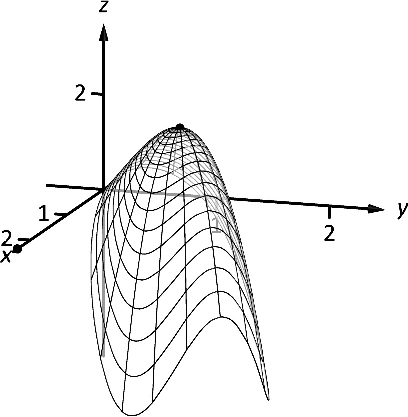
\includegraphics[width=0.5\textwidth]{fig_multi_var_19}
	\caption{Graphing $f$ in Example \ref{ex_tpl2}.}
	\label{fig_multi_var_19}
	\end{center}
\end{figure}

That is, consider any curve on the surface that goes through this point. Each curve will have a relative maximum at this point, hence its tangent line will have a slope of 0. The following section investigates the points on surfaces where all tangent lines have a slope of 0.




\end{example}


When dealing with a function $y=f(x)$ of one variable, we stated that a line through $(c,f(c))$ was tangent to $f$ if the line had a slope of $\fp(c)$ and was normal to $f$ if it had a slope of $-1/\fp(c)$. We extend the concept of normal, or orthogonal, to functions of two variables. 

Let $z=f(x,y)$ be a differentiable function of two variables. By Definition \ref{def:directional_tangent_line}, at $(x_0,y_0)$, $\ell_x(t)$ is a line parallel to the vector $\vec d_x=\left( 1,0,f_x(x_0,y_0)\right)$ and $\ell_y(t)$ is a line parallel to $\vec d_y=\left( 0,1,f_y(x_0,y_0)\right)$. Since lines in these directions through $\big(x_0,y_0,f(x_0,y_0)\big)$ are tangent to the surface, a line through this point and orthogonal to these directions would be orthogonal, or normal, to the surface. We can use this direction to create a normal line.

The direction of the normal line is orthogonal to $\vec d_x$ and $\vec d_y$, hence the direction is parallel to \linebreak $\vec d_n = \vec d_x\times \vec d_y$. It turns out this cross product has a very simple form:
$$ \vec d_x\times \vec d_y = \left( 1,0,f_x\right) \times \left( 0,1,f_y\right) = \left( -f_x,-f_y,1\right).$$
It is often more convenient to refer to the opposite of this direction, namely $\left( f_x,f_y,-1\right)$. This leads to a definition.

%\enlargethispage{3\baselineskip}

\begin{definition}[Normal line]\label{def:normal_line_space}
Let $z=f(x,y)$ be differentiable on a set $S$ containing $(x_0,y_0)$ where
$$a = f_x(x_0,y_0) \quad \text{and}\quad b=f_y(x_0,y_0)$$
are defined.\index{normal line}\index{orthogonal}\index[aut]{normaal}

\begin{enumerate}
\item	A nonzero vector parallel to $\vec n=\left( a,b,-1\right)$ is orthogonal to $f$ at $P=\big(x_0,y_0,f(x_0,y_0)\big)$.

\item The line $\ell_n$ through $P$ with direction parallel to $\vec n$ is the \textbf{normal line} (\textit{normaal}) to $f$ at $P$.
\end{enumerate}
\end{definition}

Thus the parametric equations of the normal line to a surface $f$ at $\big(x_0,y_0,f(x_0,y_0)\big)$ are:
$$\ell_{n}(t) = \left\{\begin{array}{l} x= x_0+at\\ y = y_0 + bt \\ z = f(x_0,y_0) - t. \end{array}\right.$$


The direction of the normal line has many uses, one of which is the definition of the \textbf{tangent plane} (\textit{raakvlak}) which we define shortly. Another use is in measuring distances from the surface to a point. Given a point $Q$ in space, it is a general geometric concept to define the distance from $Q$ to the surface as being the length of the shortest line segment $\vv{PQ}$ over all points $P$ on the surface. This, in turn, implies that $\vv{PQ}$ will be orthogonal to the surface at $P$. Therefore we can measure the distance from $Q$ to the surface $f$ by finding a point $P$ on the surface such that $\vv{PQ}$ is parallel to the normal line to $f$ at $P$.\\

\begin{example}\label{ex_tpl4}
Let $f(x,y) = 2-x^2-y^2$ and let $Q = (2,2,2)$. Find the distance from $Q$ to the surface defined by $f$.

\xhrulefill{gray}{2.5pt}Solution \xhrulefill{gray}{2.5pt}

From Definition~\ref{def:normal_line_space}, we know that at $(x,y)$ the direction of the normal line will be $\vec d_n = \left( -2x,-2y,-1\right)$. A point $P$ on the surface will have coordinates $(x,y,2-x^2-y^2)$, so we have $\vv{PQ} = \left( 2-x,2-y,x^2+y^2\right)$. To find where $\vv{PQ}$ is parallel to $\vec d_n$, we need to find $x$, $y$ and $c$ such that $c\vv{PQ} = \vec d_n$.
$$\begin{array}{rrcl}
 &c\vv{PQ} &=& \vec d_n \\
\Rightarrow &c\left( 2-x,2-y,x^2+y^2\right) &=& \left( -2x,-2y,-1\right)
\end{array}$$
This implies
\begin{align*}
c(2-x) &= -2x,\\
c(2-y) &= -2y,\\
c(x^2+y^2) &= -1.
\end{align*}

In each equation, we can solve for $c$:
$$c = \frac{-2x}{2-x} = \frac{-2y}{2-y} = \frac{-1}{x^2+y^2}.$$
The first two fractions imply $x=y$, and so the last fraction can be rewritten as $c=-1/(2x^2)$. Then
$$\begin{array}{rrcl}
 & \dfrac{-2x}{2-x}& = & \dfrac{-1}{2x^2} \\[0.2cm]
\Leftrightarrow  & -2x(2x^2) & = & -1(2-x) \\[0.2cm]
\Leftrightarrow  & 4x^3 & = & 2-x\\[0.2cm]
\Leftrightarrow  & 4x^3+x-2 &= & 0.
\end{array}$$
This last equation is a cubic, which is not difficult to solve with a numeric solver. We find that $x\approx 0.689$, hence $P = (0.689,0.689, 1.051)$. We find the distance from $Q$ to the surface of $f$ is 
$$\norm{\vv{PQ}} = \sqrt{(2-0.689)^2 +(2-0.689)^2+(2-1.051)^2} = 2.083.$$ 
\end{example}


We can of course take the concept of measuring the distance from a point to a surface to find a point $Q$ a particular distance from a surface at a given point $P$ on the surface.

\subsection{Tangent plane}
We can use the direction of the normal line to define a plane. With $a=f_x(x_0,y_0)$, $b=f_y(x_0,y_0)$ and $P = \big(x_0,y_0,f(x_0,y_0)\big)$, the vector $\vec n=\left( a,b,-1\right)$ is orthogonal to $f$ at $P$. The plane through $P$ with normal vector $\vec n$ is therefore tangent to $f$ at $P$.
	\checkoddpage
\marginpar{\ifoddpage\hspace*{-1.5cm}\else\hspace*{0.25cm}\fi
\includegraphics[width=0.075\textwidth]{icon_demo}}


\begin{definition}[Tangent plane]\label{def:tangent_plane}
Let $z=f(x,y)$ be differentiable on a set $S$ containing $(x_0,y_0)$, where
$a = f_x(x_0,y_0)$, $b=f_y(x_0,y_0)$, $\vec n= \left( a,b,-1\right)$ and $P=\big(x_0,y_0,f(x_0,y_0)\big)$.\\

The plane through $P$ with normal vector $\vec n$ is the \textbf{tangent plane to $f$ at $P$} (\textit{raakvlak aan $f$ in $P$}). The standard form of this plane is 
\index{tangent plane}\index{planes!tangent}\index[aut]{raakvlak}
\begin{eqnarray*}
\vec{n}\cdot\left((x-x_0),(y-y_0),(z-f(x_0,y_0))\right)&=&0\\
\Leftrightarrow\qquad a(x-x_0) + b(y-y_0) - \big(z-f(x_0,y_0)\big)&=&0.
\end{eqnarray*}
\end{definition}


\ifcalculus\pagebreak\fi
\begin{example}\label{ex_tpl6}
Find the equation of the normal line and tangent plane to $z=-x^2-y^2+2$ at $(0,1)$.

\pagebreak
\xhrulefill{gray}{2.5pt}Solution \xhrulefill{gray}{2.5pt}

We find $z_x(x,y) = -2x$ and $z_y(x,y) = -2y$; at $(0,1)$, we have $z_x = 0$ and $z_y = -2$. We take the direction of the normal line, following Definition \ref{def:normal_line_space}, to be $\vec n=\left( 0,-2,-1\right)$. The line with this direction going through the point $(0,1,1)$ is 
$$\ell_n(t) = \left\{\begin{array}{l} x=0\\y=1-2t\\z=1-t\end{array}\right.\quad \text{or}\quad \ell_n(t)=\left( 0,1,1\right)+\left( 0,-2,-1\right) t.$$
The surface $z=-x^2-y^2+2$, along with the found normal line, is graphed in Figure \ref{fig_multi_var_20a}. 

Since we have that $\vec n = \left( 0,-2,-1\right)$ and $P = (0,1,1)$,  the equation of the tangent plane is 
$$-2(y-1)-(z-1)=0.$$
The surface $z=-x^2-y^2+2$ and tangent plane are graphed in Figure \ref{fig_multi_var_20b}. 

\begin{figure}[H]
\centering
%\raisebox{0.5cm}{
\subfigure[\label{fig_multi_var_20a}]{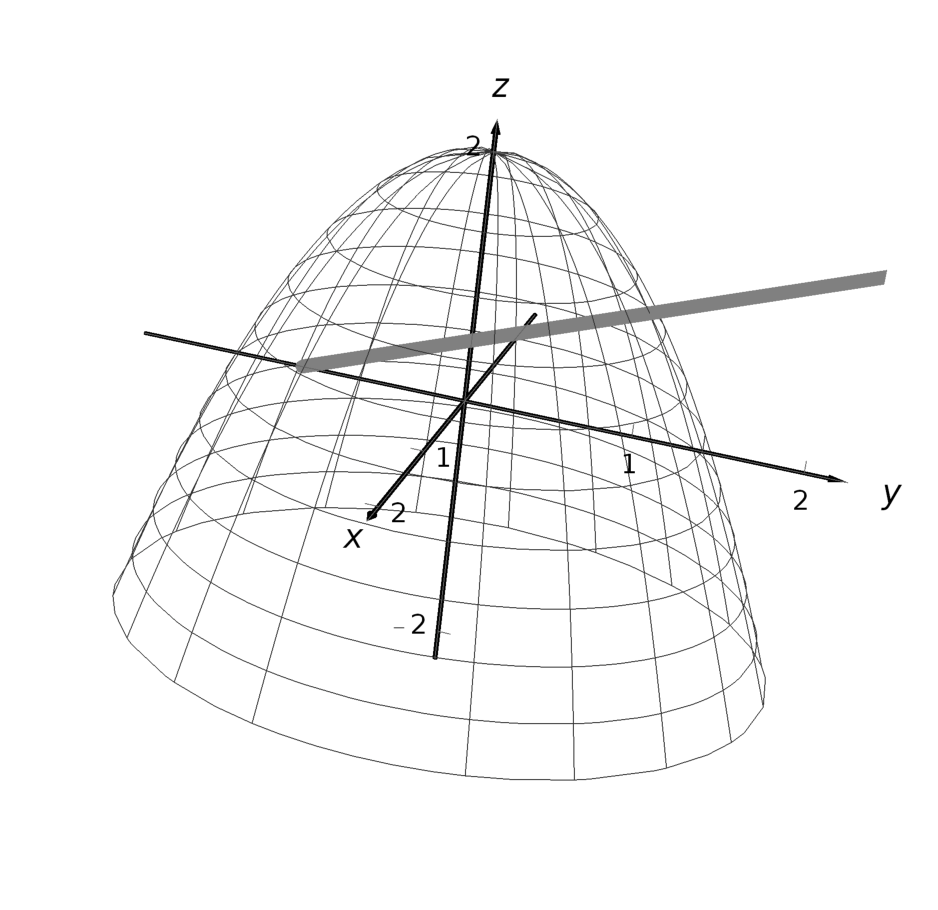
\includegraphics[width=0.43\textwidth]{fig_multi_var_20a}}
\qquad
\subfigure[\label{fig_multi_var_20b}]{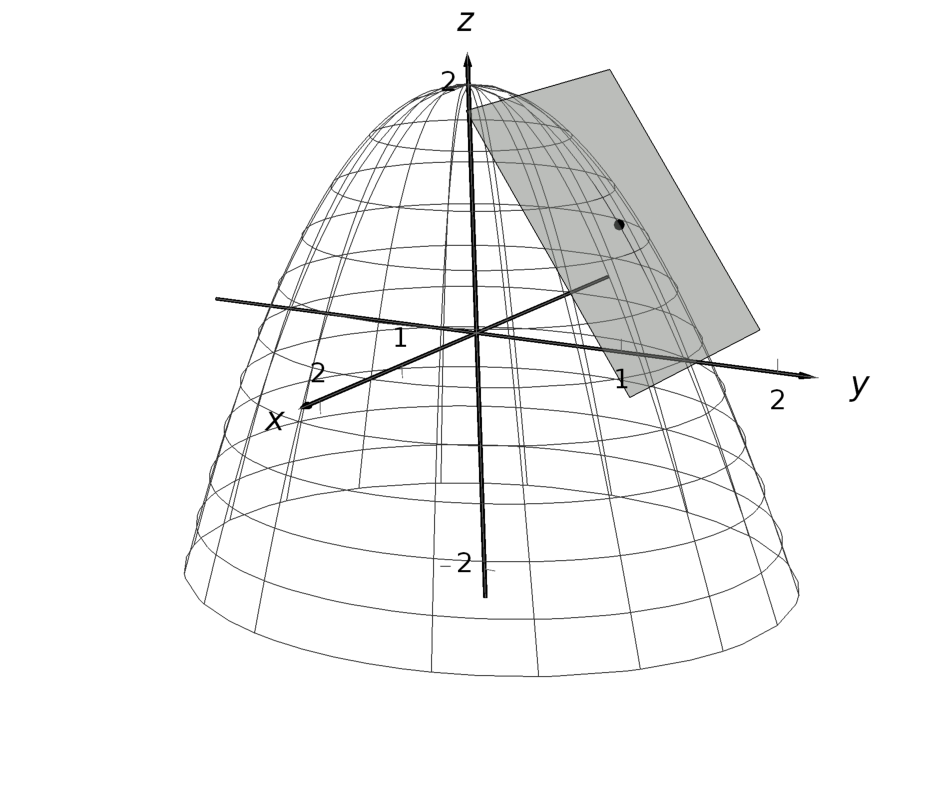
\includegraphics[width=0.43\textwidth]{fig_multi_var_20b}}
\caption{Graphing a surface with  normal line and tangent plane from Example \ref{ex_tpl6}.}
\end{figure}
\end{example}


Just as tangent lines can be used to approximate function values of functions of one variable, tangent planes can be used to achieve this for functions of two variables. 


\begin{example}\label{ex_tpl7}
The point $(3,-1,4)$ lies on the surface of an unknown differentiable function $f$ where $f_x(3,-1) = 2$ and $f_y(3,-1) = -1/2$. Find the equation of the tangent plane to $f$ at $P$, and use this to approximate the value of $f(2.9,-0.8)$.

\xhrulefill{gray}{2.5pt}Solution \xhrulefill{gray}{2.5pt}

Knowing the partial derivatives at $(3,-1)$ allows us to form the normal vector to the tangent plane, $\vec n = \left( 2,-1/2,-1\right)$. Thus the equation of the tangent line to $f$ at $P$ is:
\begin{equation}
2(x-3)-\dfrac{1}{2}(y+1) - (z-4) = 0 \quad \Leftrightarrow \quad z = 2(x-3)-\dfrac{1}{2}(y+1)+4.\label{eq:tpl7}\end{equation}
Just as tangent lines provide excellent approximations of curves near their point of intersection, tangent planes provide excellent approximations of surfaces near their point of intersection. So $f(2.9,-0.8) \approx z(2.9,-0.8) = 3.7.$

This is not a new method of approximation. Compare the right hand expression for $z$ in Equation \eqref{eq:tpl7} to the total differential:
$$dz = f_xdx + f_ydy \quad \text{and} \quad z = \underbrace{\underbrace{2}_{f_x}\underbrace{(x-3)}_{dx}+\underbrace{-1/2}_{f_y}\underbrace{(y+1)}_{dy}}_{dz}+4.$$
Thus the new $z$-value is the sum of the change in $z$ (i.e., $dz$) and the old $z$-value (4). As mentioned when studying the total differential, it is not uncommon to know partial derivative information about an unknown function $f$, and tangent planes are used to give accurate approximations of $f$.
\end{example}


Recall that when $w=f(x,y,z)$, the gradient $\vec{\nabla} f = \left( f_x,f_y,f_z\right)$ is orthogonal to level surfaces of $f$. Given a point $(x_0,y_0,z_0)$, let $c = f(x_0,y_0,z_0)$. Then $f(x,y,z) = c$ is a level surface that contains the point $(x_0,y_0,z_0)$ and $\vec{\nabla} f(x_0,y_0,z_0)$ is orthogonal to this level surface. So, the gradient at a point gives a vector orthogonal to the surface at that point. This direction can be used to find tangent planes and normal lines.

\begin{example}\label{ex_tpl8}
Find the equation of the plane tangent to the ellipsoid $$\ds \frac{x^2}{12} +\frac{y^2}{6}+\frac{z^2}{4}=1$$ at $P = (1,2,1)$.

\xhrulefill{gray}{2.5pt}Solution \xhrulefill{gray}{2.5pt}

We consider the equation of the ellipsoid as a level surface of a function $F$ of three variables, where $F(x,y,z) = \frac{x^2}{12} +\frac{y^2}{6}+\frac{z^2}{4}$.  The gradient is:
\begin{align*}
\vec{\nabla} F(x,y,z) &= \left( F_x, F_y,F_z\right) \\
			&= \left( \frac x6, \frac y3, \frac z2\right).
\end{align*}
At  $P$, the gradient is $\vec{\nabla} F(1,2,1) = \left( 1/6, 2/3, 1/2\right)$. Thus the equation of the plane tangent to the ellipsoid at $P$ is
$$\frac 16(x-1) + \frac23(y-2) + \frac 12(z-1) = 0.$$ The ellipsoid and tangent plane are graphed in Figure \ref{fig_multi_var_21}.

\begin{figure}[H]
	\begin{center}
			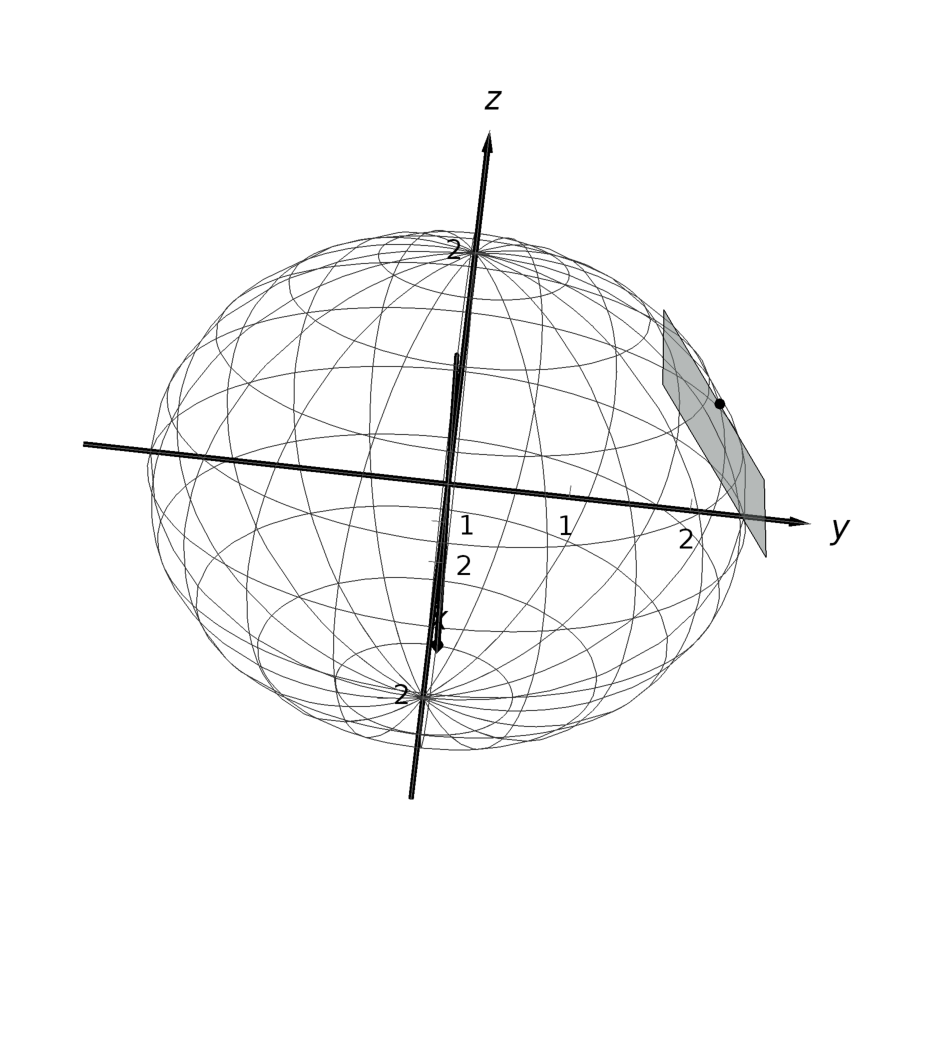
\includegraphics[width=0.5\textwidth]{fig_multi_var_21}
	\caption{An ellipsoid and its tangent plane at a point.}
	\label{fig_multi_var_21}
	\end{center}
\end{figure}

\end{example}

Tangent lines and planes to surfaces have many uses, including the study of instantaneous rates of changes and making approximations. Normal lines also have many uses. In this section we focused on using them to measure distances from a surface. Another interesting application is in computer graphics, where the effects of light on a surface are determined using normal vectors.

The next section investigates another use of partial derivatives: Taylor series expansions of functions of several variables.

\section{Taylor series expansions}\label{sec:taylor_multi_var}
Recall that we found in Section~\ref{sec:taylor_series} a way of rewriting a continuous function of one variable as a series by relying on Taylor's theorem. Having introduced all mathematical tools that are needed to analyse functions of several variables, we are now ready to introduce Taylor's theorem for a function of two variables.

\begin{theorem}[Taylor's theorem for a function of two variables]\label{thm:taylor2thm}
Let $f$ be a $C^{n+1}$ function on a set $D$ containing $(x_0,y_0)$. Then, for each $(x,y)$ in $D$, there exists $(\theta_x,\theta_y)$ between $(x,y)$ and $(x_0,y_0)$ such that
\begin{equation*}
f(x,y) =\sum_{i=0}^n\dfrac{1}{i!}\left(\dfrac{\partial}{\partial x}(x-x_0)+\dfrac{\partial}{\partial y}(y-y_0)\right)^i f(x_0,y_0)+R_n(x,y)\,,
\end{equation*}
where
\begin{multline*}
f(x,y)=f(x_0,y_0)+\dfrac{1}{1!}f_x(x_0,y_0)(x-x_0)+\dfrac{1}{1!}f_y(x_0,y_0)(y-y_0)+\dfrac{1}{2!}f_{xx}(x_0,y_0)(x-x_0)^2+\\[0.2cm]
\dfrac{2}{2!} f_{xy}(x_0,y_0)(x-x_0)(y-y_0)+\dfrac{1}{2!}f_{yy}(x_0,y_0)(y-y_0)^2+\ldots
\end{multline*}
and the remainder term is given by
$$
R_n(x,y)=\dfrac{1}{(n+1)!}\left(\dfrac{\partial}{\partial x}(x-x_0)+\dfrac{\partial}{\partial y}(y-y_0)\right)^{n+1}f(\theta_x,\theta_y).
$$
\index{Taylor Polynomial!Taylor's Theorem}\index{Taylor's Theorem}

\end{theorem}

%More explicitly, this theorem allows us to write a function $f(x,y)$ at a point $(x_0,y_0)$ as
%\begin{multline*}
%f(x,y)=f(x_0,y_0)+\dfrac{1}{1!}f_x(x_0,y_0)(x-x_0)+\dfrac{1}{1!}f_y(x_0,y_0)(y-y_0)+\dfrac{1}{2!}f_{xx}(x_0,y_0)(x-x_0)^2+\\[0.2cm]
%\dfrac{2}{2!} f_{xy}(x_0,y_0)(x-x_0)(y-y_0)+\dfrac{1}{2!}f_{yy}(x_0,y_0)(y-y_0)^2+\ldots
%\end{multline*}

\ifanalysis


\begin{proof}
For the sake of brevity, we will restrict the proof to functions of two variables, though the same reasoning may be followed to arrive at a full proof of the $n$ variables case. 

Essentially, the proof starts off in a similar way as the one of the mean value theorem for functions of $n$ variables (Theorem~\ref{thm:mvtmulti})  by devising an appropriate one-variable function to which we can apply Taylor's theorem of functions of one variable (Theorem~\ref{thm:taylorthm}).

We start by considering a point in the neighbourhood of $(x_0,y_0)$. Let us say, the point  $(x_0+\Delta x,y_0+\Delta y)$ and we then look for a formula for $f(x_0+\Delta x,y_0+\Delta y)$. As we will try to use Taylor's theorem for functions of one variable, we consider the  vector-valued function $\vec{\phi}:\mathbb{R}\mapsto\mathbb{R}^2$ of one variable:
$$
\vec{\phi}(t)=(x_0+t\Delta x,y_0+t\Delta y)
$$
for $t\in[0,1]$, which traces out the line segment connecting $(x_0,y_0)$ and $(x_0+\Delta x,y_0+\Delta y)$. Subsequently, we consider the composition
$$
g=f\circ\,\vec{\phi}\,,
$$
which is $C^{n+1}$ in agreement with what we concluded in the proof of Theorem~\ref{thm:mvtmulti}. Consequently, we may apply Taylor's theorem of functions of one variable to $g$, meaning that for every $t\in[0,1]$ there exists a $\theta_t\in]0,1[$ such that
\begin{equation}
g(t)=g(0) + g'(0)t + \frac{g''(0)}{2!}t^2+ \cdots +\frac{g\,^{(n)}(0)}{n!}t^n+R_n(t)\,,
\label{taylormulti_stap1}
\end{equation}
where 
$$\ds R_n(t) = \frac{g\,^{(n+1)}(\theta_t)}{(n+1)!}t^{(n+1)}.$$
Now, note that
$$
g(0)=f(x_0,y_0)\qquad\text{and}\qquad\,g(1)=f(x_0+\Delta x,y_0+\Delta y)\,,
$$
while the higher-order derivatives in Equation~\eqref{taylormulti_stap1} can be obtained using the chain rule. In this way, we obtain
\allowdisplaybreaks
\begin{eqnarray*}
g(t)&=&f(x_0+t\Delta x,y_0+t\Delta y)\\
g'(t)&=&\Delta x\dfrac{\partial f}{\partial x}(x_0+t\Delta x,y_0+t\Delta y)+\Delta y\dfrac{\partial f}{\partial y}(x_0+t\Delta x,y_0+t\Delta y)\\[0.2cm]
&=&\left(\Delta x\dfrac{\partial}{\partial x}+\Delta y\dfrac{\partial}{\partial y}\right)f(x_0+t\Delta x,y_0+t\Delta y)\\[0.2cm]
g''(t)&=&\Delta x^2\dfrac{\partial^2 f}{\partial x^2}(x_0+t\Delta x,y_0+t\Delta y)+2\Delta x\Delta y\dfrac{\partial^2 f}{\partial x\partial y}(x_0+t\Delta x,y_0+t\Delta y)+\Delta y^2\dfrac{\partial^2 f}{\partial y^2}(x_0+t\Delta x,y_0+t\Delta y)\\[0.2cm]
&=&\left(\Delta x\dfrac{\partial}{\partial x}+\Delta y\dfrac{\partial}{\partial y}\right)^2f(x_0+t\Delta x,y_0+t\Delta y)\\[0.2cm]
&\ldots&\\
g^{(n)}(t)&=&\left(\Delta x\dfrac{\partial}{\partial x}+\Delta y\dfrac{\partial}{\partial y}\right)^nf(x_0+t\Delta x,y_0+t\Delta y)
\end{eqnarray*}
More specifically, we immediately get
$$
g^{(n)}(0)=\left(\Delta x\dfrac{\partial}{\partial x}+\Delta y\dfrac{\partial}{\partial y}\right)^nf(x_0,y_0)\,.
$$
Consequently, choosing $t=1$ in Equation~\eqref{taylormulti_stap1} we arrive at 
\begin{multline*}
g(1)=f(x_0+\Delta x,y_0+\Delta y)=f(x_0,y_0)+\left(\Delta x\dfrac{\partial}{\partial x}+\Delta y\dfrac{\partial}{\partial y}\right)f(x_0,y_0)+\cdots\\[0.2cm]
+\dfrac{1}{2!}\left(\Delta x\dfrac{\partial}{\partial x}+\Delta y\dfrac{\partial}{\partial y}\right)^2f(x_0,y_0)+ \cdots +
\dfrac{1}{n!}\left(\Delta x\dfrac{\partial}{\partial x}+\Delta y\dfrac{\partial}{\partial y}\right)^nf(x_0,y_0)+R_n(x,y)\,,
\end{multline*}
where
$$
R_n(x,y)=\dfrac{1}{(n+1)!}\left(\Delta x\dfrac{\partial}{\partial x}+\Delta y\dfrac{\partial}{\partial y}\right)^{n+1}f(x_0+\theta_t\Delta x,y_0+\theta_t\Delta y)\,.
$$
Finally, acknowledging that $\Delta x=x-x_0$ and $\Delta y=y-y_0$, we can restate the previous expression as
\begin{multline*}
g(1)=f(x,y)=f(x_0,y_0)+\left((x-x_0)\dfrac{\partial}{\partial x}+(y-y_0)\dfrac{\partial}{\partial y}\right)f(x_0,y_0)+\cdots\\[0.2cm]
+\dfrac{1}{2}\left((x-x_0)\dfrac{\partial}{\partial x}+(y-y_0)\dfrac{\partial}{\partial y}\right)^2f(x_0,y_0)+ \cdots +
\dfrac{1}{n!}\left((x-x_0)\dfrac{\partial}{\partial x}+(y-y_0)\dfrac{\partial}{\partial y}\right)^nf(x_0,y_0)+R_n(x,y)\,,
\end{multline*}
$$
R_n(x,y)=\dfrac{1}{(n+1)!}\left((x-x_0)\dfrac{\partial}{\partial x}+(y-y_0)\dfrac{\partial}{\partial y}\right)^{n+1}f(\theta_x,\theta_y)\,,
$$
where $\theta_x=x_0+\theta_t(x-x_0)$ and $\theta_y=y_0+\theta_t(y-y_0)$.
\end{proof}

\fi

As for functions of one variable, the Talor polynomial of degree $n$ provides the best $n$-th degree polynomial approximation of $f(x,y)$ near a point $(x_0,y_0)$. For instance, letting $n=1$, we obtain
$$
f(x,y)\approx f(x_0,y_0)+f_x(x_0,y_0)(x-x_0)+f_y(x_0,y_0)(y-y_0).
$$

\begin{example}
Find a second-degree polynomial approximation to the function
$$
f(x,y)=\sqrt{x^2+y^3}
$$
near the point $(1,2)$ and use it to estimate the value of $\sqrt{1.02^2+1.97^3}$.

\xhrulefill{gray}{2.5pt}Solution \xhrulefill{gray}{2.5pt}

For a second-degree approximation we need the values of the partial derivatives of $f$ up to the second order at the point $(1,2)$. We have

$$
\renewcommand{\arraystretch}{1.5}
\begin{tabular}{rcl|crcl}
\multicolumn{3}{c}{Derivative function}&\multicolumn{3}{c}{Derivative at $(1,2)$}\\\hline
$f(x,y)$      & = & $\sqrt{x^2+y^3}$ &  &  $f(1,2)$&=&$3$\\
$f_x(x,y)$    & = & $\dfrac{x}{\sqrt{x^2+y^3}}$ &  & $f_x(1,2)$    & = & $\dfrac{1}{3}$\\
$f_y(x,y)$    & = & $\dfrac{3y^2}{2\sqrt{x^2+y^3}}$ &  & $f_x(1,2)$ & = & $2$\\
$f_{xx}(x,y)$ & = & $\dfrac{y^3}{\left(x^2+y^3\right)^{3/2}}$ &  &  $f_{xx}(1,2)$ & = & $\dfrac{8}{27}$\\
$f_{xy}(x,y)$& = & $\dfrac{-3xy^2}{2\left(x^2+y^3\right)^{3/2}}$&  &  $f_{xy}(1,2)$& = & $-\dfrac{2}{9}$\\
$f_{yy}(x,y)$& = &$\dfrac{12x^2y+3y^4}{4\left(x^2+y^3\right)^{3/2}}$&  & $f_{yy}(1,2)$& = &$\dfrac{2}{3}$.\\
\end{tabular}
\renewcommand{\arraystretch}{1}
$$
Thus, we get after evaluating the partial derivatives in $(1,2)$
$$
f(x,y)\approx 3+\dfrac{1}{3}(x-1)+2(y-2)+\dfrac{4}{27}(x-1)^2-\dfrac{2}{9}(x-1)(y-2)+\dfrac{1}{3}(y-2)^2.
$$
This is the required second-degree Taylor polynomial for $f$ near $(1,2)$. Therefore,
\begin{eqnarray*}
\sqrt{1.02^2+1.97^3}&=&f(1+0.02,2-0.03)\\[0.2cm]
&\approx&3+\dfrac{1}{3}(0.02)+2(-0.03)+\dfrac{4}{27}(0.02)^2-\dfrac{2}{9}(0.02)(-0.03)+\dfrac{1}{3}(-0.03)^2\\[0.2cm]
&\approx&2.9471593.
\end{eqnarray*}
\ifanalysis It can be verified that the true value is 2.9471636, so our approximation is accurate to six significant figures. \fi

\end{example}


	\checkoddpage
\marginpar{\ifoddpage\hspace*{-1.5cm}\else\hspace*{0.25cm}\fi
\includegraphics[width=0.075\textwidth]{youtube}\\
\ifoddpage\hspace*{-1.75cm}\else\hspace*{0.1cm}\fi
\qrcode[height=1.75cm]{https://youtu.be/JEvGbsl8hXw}
%\includegraphics[width=0.1\textwidth]{taylor_multi}
}

Clearly, in line with what we devised for functions of one variable, the Taylor series expansion of a function of two variables is given by
$$
f(x,y) =\sum_{i=0}^{+\infty}\dfrac{1}{i!}\left(\dfrac{\partial}{\partial x}(x-x_0)+\dfrac{\partial}{\partial y}(y-y_0)\right)^i f(x_0,y_0),$$
and likewise a Maclaurin series expansion can be formulated.


\begin{example}
Find a second-order Taylor series expansion of the function
$$
\displaystyle f(x,y)=e^{x}\ln(1+y),
$$
around the point $(0, 0)$. 

\xhrulefill{gray}{2.5pt}Solution \xhrulefill{gray}{2.5pt}

In order to compute a second-order Taylor series expansion we first compute the necessary partial derivatives and evaluate these derivatives at the origin:
\begin{center}
\renewcommand{\arraystretch}{1.5}
\begin{tabular}{rcl|crcl}
\multicolumn{3}{c}{Derivative function}&\multicolumn{3}{c}{Derivative at $(0,0)$}\\\hline
$f_{x}(x,y)$ & =&$e^{x}\ln(1+y)$& &$f_{x}(0,0)$& =&$0$\\[6pt]
$f_{y}(x,y) $& =& ${\dfrac {e^{x}}{1+y}}$&  &$f_{y}(0,0)$& =&$1$\\[6pt]
$f_{xx}(x,y)$& =& $e^{x}\ln(1+y)$&  & $f_{xx}(0,0)$&=&$0$\\[6pt]
$f_{xy}(x,y)$& =& $f_{yx} = {\dfrac {e^{x}}{1+y}}$ &  &$f_{xy}(0,0)$& =&$1$\\[6pt]
$f_{yy}(x,y)$& =& $-{\dfrac {e^{x}}{(1+y)^{2}}}$ &  &$f_{yy}(0,0)$& =&$ -1$
\end{tabular}
\renewcommand{\arraystretch}{1}
\end{center}


%Evaluating these derivatives at the origin gives the Taylor coefficients 
%$$
%\displaystyle {\begin{aligned}
%f_{x}(0,0)&=0\\
%f_{y}(0,0)&=1\\
%f_{xx}(0,0)&=0\\
%f_{yy}(0,0)&=-1\\
%f_{xy}(0,0)&=f_{yx}(0,0)=1.
%\end{aligned}
%}
%$$

Relying on Taylor's theorem, this leads to
$$
\displaystyle {\begin{aligned}f(x,y)&=0+0(x-0)+1(y-0)+{\frac {1}{2}}{\Big (}0(x-0)^{2}+2(x-0)(y-0)+(-1)(y-0)^{2}{\Big )}+\cdots \\&=y+xy-{\frac {y^{2}}{2}}+\cdots \end{aligned}}.
$$
Finally, we have
$$
\displaystyle e^{x}\ln(1+y)=y+xy-{\frac {y^{2}}{2}}+\cdots
$$
for $y>-1$.


\end{example}



\ifanalysis
Of course, Taylor series expansions may be extended to functions of $n$ variables. 
\fi
\ifcalculus
Of course, Taylor series expansions may be extended to functions of 3 variables. 
\fi


\section{Extreme values}\label{sec:multi_extreme_values}
\ifcalculus
In this section we discuss the basic concepts for analyzing extrema of functions of several variables. This will provide us a number of tools that are extremely useful for solving practical engineering problems, such as cost reduction in economics, yield optimization in synthetic biology or learning from data in artificial intelligence, to name just a few. For simplicity we will first discuss functions of two variables, for which concepts can be graphically visualized, before moving to functions of \ifanalysis several\fi \ifcalculus three \fi variables, for which things get a bit more abstract and less intuitive. We start by analyzing necessary conditions for extrema (i.e.\ conditions that must hold for a point to be a candidate for an extremum), before moving to sufficient conditions (i.e.\ if such conditions hold, then we are sure that we have an extremum). 


\subsection{Necessary conditions for extrema}
\label{FTV}

Figure~\ref{fig_multi_var_22} shows two functions of two variables. The function $f(x,y) = x^2 + y^2$ obviously has a minimum value of $0$ (Figure~\ref{fig_multi_var_22a}). This minimum value is found in the point $(x=0,y=0)$. Conversely, the function $g(x,y) = 1 - x^2 - y^2$ has a maximum value at $(x=0,y=0)$ (Figure~\ref{fig_multi_var_22b}). At this point $g(0,0)=1$, while $g$ has a smaller value for any other point of its domain. What techniques could be used to find such minima and maxima, if they were not immediately visible from a plot? 


\begin{figure}
\centering
%\raisebox{0.5cm}{
\subfigure[\label{fig_multi_var_22a}]{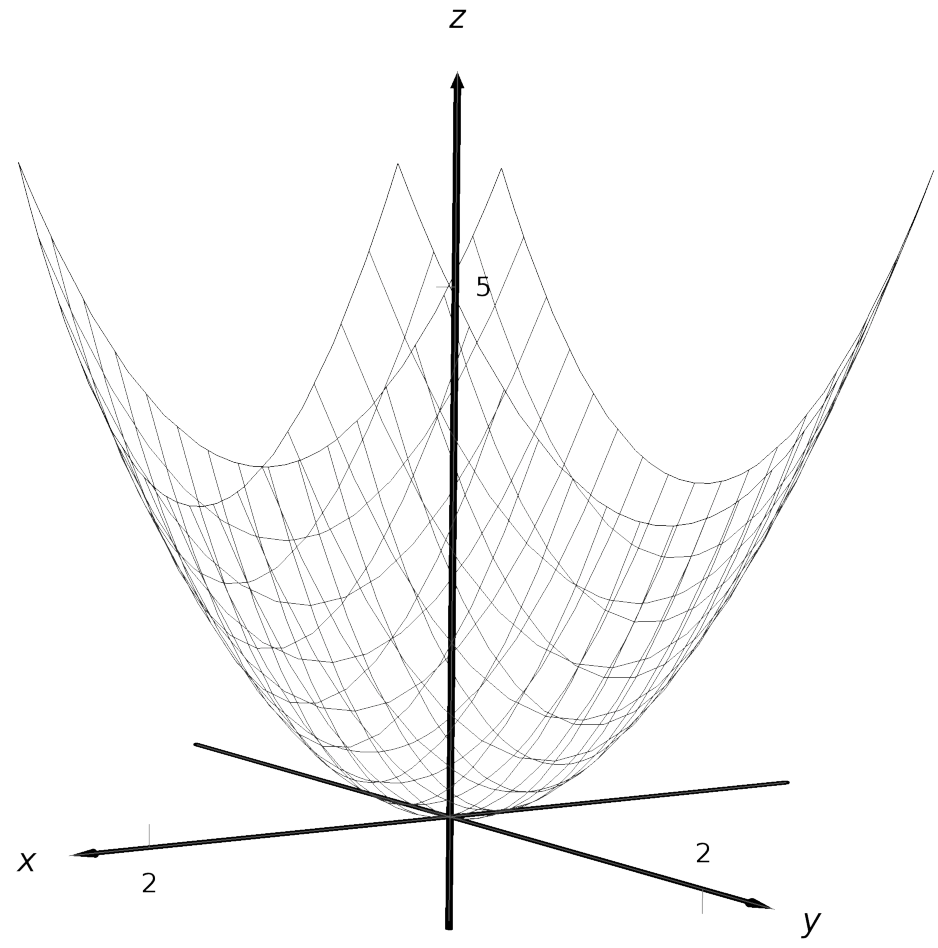
\includegraphics[width=0.43\textwidth]{fig_multi_var_22a}}
\qquad
\subfigure[\label{fig_multi_var_22b}]{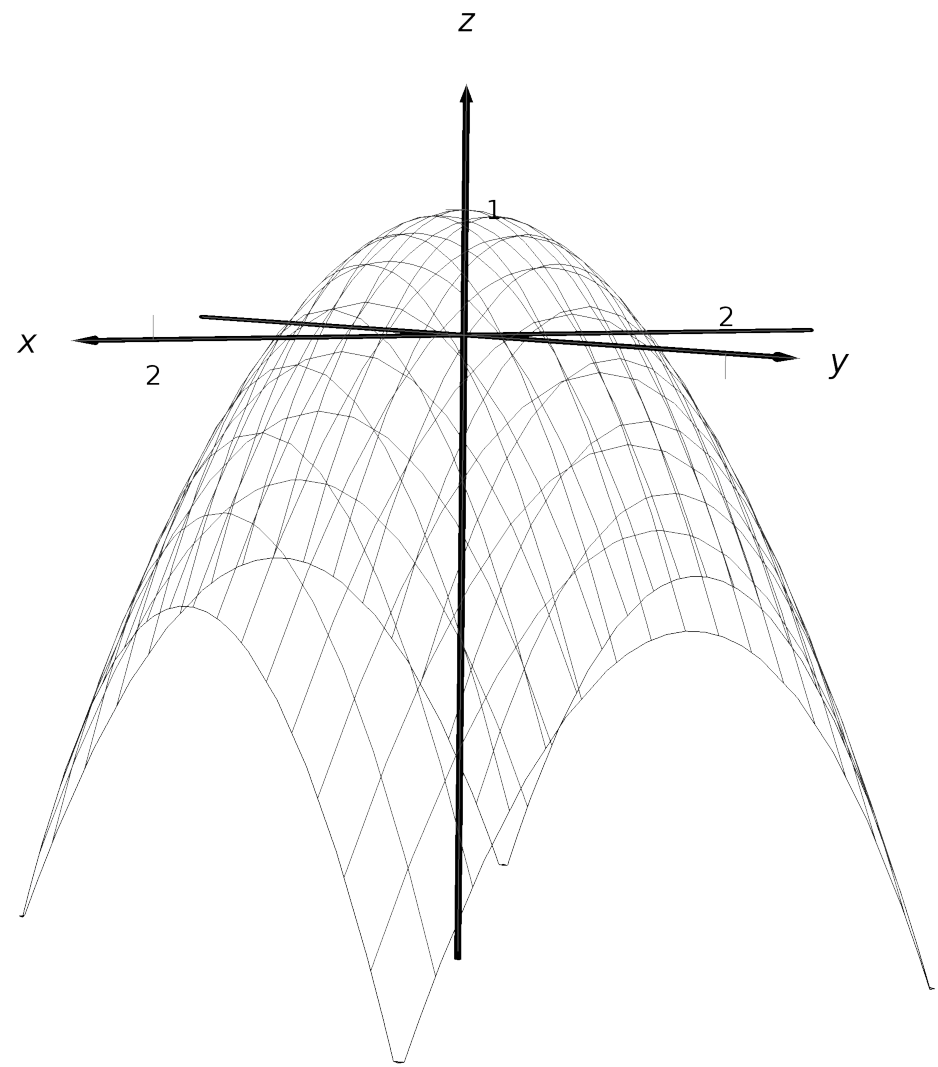
\includegraphics[width=0.43\textwidth]{fig_multi_var_22b}}
\caption{A plot of two simple functions that have  a single  minimum (a) and maximum (b). \label{fig_multi_var_22}}
\end{figure}

Unfortunately, the techniques for finding the minima and maxima of functions of several variables are substantially more complicated than those for functions of one variable.

First of all, we formalise the notion relative and absolute extrema of a function of two variables in agreement with the definition given for functions of one variable (Definitions~\ref{def:extreme_values} and \ref{def:rel_ext}). 

\begin{definition}[Relative and absolute extrema]\label{def:multi_extrema}
Let $z=f(x,y)$ be defined on a set $S$ containing the point $P=(x_0,y_0)$.
\begin{enumerate}
	\item	If $f(x_0,y_0)\geq f(x,y)$ for all $(x,y)$ in $S$, then $f$ has an \textbf{absolute maximum} (\textit{globaal maximum}) at $P$.
	
	If $f(x_0,y_0)\leq f(x,y)$ for all $(x,y)$ in $S$, then $f$ has an \textbf{absolute minimum} (\textit{globaal minimum}) at $P$.
	
	\item If there is an open disk $D$ containing $P$ such that $f(x_0,y_0) \geq f(x,y)$ for all points $(x,y)$ that are in both $D$ and $S$, then $f$ has a \textbf{relative maximum} (\textit{lokaal maximum}) at $P$.
	
	If there is an open disk $D$ containing $P$ such that $f(x_0,y_0) \leq f(x,y)$ for all points $(x,y)$ that are in both $D$ and $S$, then $f$ has a \textbf{relative minimum} (\textit{lokaal minimum}) at $P$.
	
	
	\item		If $f$ has an absolute maximum or minimum at $P$, then $f$ has an \textbf{absolute extremum} at $P$.
	
	If $f$ has a relative maximum or minimum at $P$, then $f$ has a \textbf{relative extremum} at $P$.
	
	
\end{enumerate}
\index{function ! (absolute) maximum}\index[aut]{functie ! (absoluut) maximum}
\index{function ! (absolute) minimum}\index[aut]{functie ! (absoluut) minimum}
\index{extreme values}\index[aut]{extreme waarden}
\index{absolute maximum}\index[aut]{absoluut maximum}
\index{absolute minimum}\index[aut]{absoluut minimum}
\index{maximum}\index[aut]{maximum}
\index{minimum}\index[aut]{minimum}
\index{extrema}\index[aut]{extrema}
\index{extremum}\index[aut]{extremum}
\end{definition}

 Similarly to functions of one variable, $z=f(x,y)$ can have an extremum in critical and singular points and in the end points of the domain of $f$, in situations where the domain is not $\mathbb{R}$.  Critical points of functions of two variables are defined as follows. 

\begin{definition}[Critical point]\label{def:multi_critical_point}
Let $z = f(x,y)$ be continuous on a set $S$. A \textbf{critical point} (\textit{kritisch punt}) $P=(x_0,y_0)$ of $f$ is a point in $S$ such that, at $P$,\index{critical point}\index[aut]{kritisch punt}
$$
f_x(x_0,y_0) = 0 \qquad \text{ and } \qquad f_y(x_0,y_0) = 0\,..
$$
\end{definition}

Besides, when $f_x(x_0,y_0)$ and/or $f_y(x_0,y_0)$ is undefined, we call $P=(x_0,y_0)$ a \textbf{singular point} (\textit{singulier punt}), just as we did within the framework of functions of one variable (Definition~\ref{def:singularnum}). \index{singular point}



In what follows we will present methods to find local minima or maxima. The determination of global minima and maxima becomes a trivial task once the local minima and maxima are found. The global minima are simply the points with minimal value among the local mimina (usually we have a single global minimum, the exception is the case where two or more points have exactly the same minimal value). Likewise, the global maxima are the points with maximal value among the local maxima. Figure~\ref{fig_multi_var_23} shows a plot of a function of two variables where local and global extrema are distinguished. 

\begin{figure}
\centering
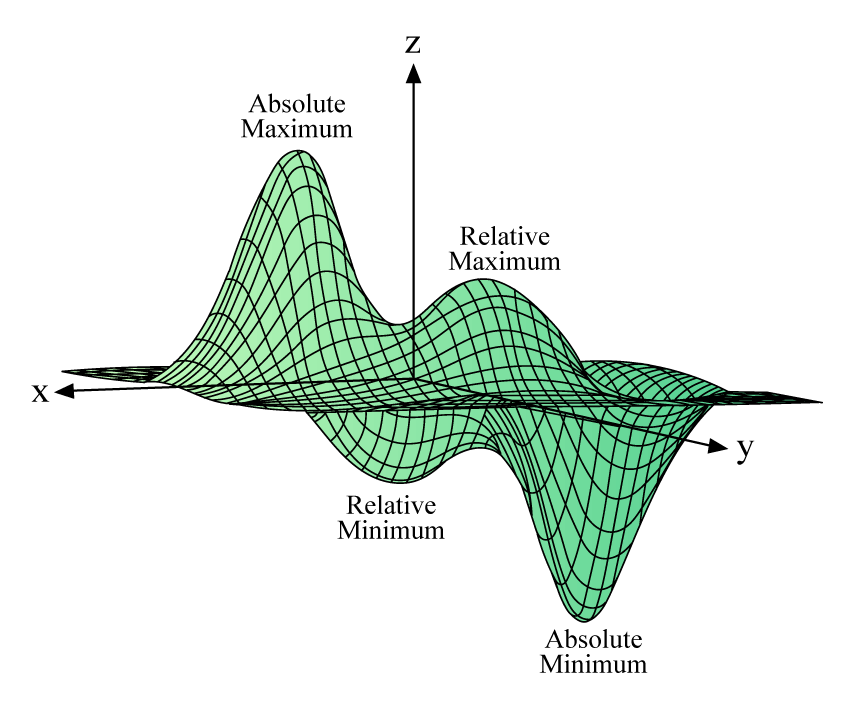
\includegraphics[scale=1]{fig_multi_var_23.png} 
\caption{A plot of a function with more than one local minimum and maximum. The global minimum and maximum are indicated.}
\label{fig_multi_var_23}
\end{figure}


If $f$ has a relative or absolute maximum at $P=(x_0,y_0)$, it means that every curve on the surface of $f$ through $P$ will also have a relative or absolute maximum at $P$. Recalling what we learned in Section \ref{sec:extreme_values}, the slopes of the tangent lines to these curves at $P$ must be 0 or undefined. Since directional derivatives are computed using $f_x$ and $f_y$, we are led to the following theorem.

\pagebreak
\begin{theorem}[Necessary Conditions for Extreme Values]\label{NCFE}
A function $f(x,y)$ can have a local extremum in a point $(a,b)$ of its domain only if $(a,b)$ is one of the following:  
\begin{enumerate}
\item a critical point, i.e., a point where $\vec{\nabla} f(a,b)=\vec{0}$;
\item a singular point, i.e., a point where $\vec{\nabla} f(a,b)$ does not exist;
\item an end point of the domain of $f$.
\end{enumerate}
\end{theorem}

\ifanalysis

\begin{proof}
The proof goes as follows. Suppose $(a,b)$ belongs to the domain of $f$. If $(a,b)$ is not an end point of the domain, then it must be an interior point of the domain. If $(a,b)$ is not a singular point, then the gradient in $(a,b)$ exists.  
In your calculus course you have learned that the gradient $\vec{\nabla} f(a,b)$ defines the direction of steepest increase of the function $f $ in $(a,b)$. Also, the opposite direction (so, an angle of 180 degrees) defines the direction of steepest decrease in that point. As a result, if $(a,b)$ is not a critical point, then the function increases in $(a,b)$ in the direction of the gradient, and the function decreases in the opposite direction. So, in that case $(a,b)$ cannot be a local minimum or a local maximum. Hence the only candidate local minima and maxima are the critical points, singular points and end points of the domain.
\end{proof}

\fi

In this section we will only consider functions with an unrestricted domain. 
Therefore, to find local extrema, we find the critical and singular points of $f$ and determine which correspond to local maxima, local minima, or neither. The examples below will demonstrate this process. For functions with a restricted domain, the analysis will be require specific techniques, which are discussed in the next chapter. Also, remark that Theorem~\ref{NCFE} remains valid for functions of more than two variables, with identical arguments as the ones given in its proof. 

\begin{example}\label{ex_multi_extreme2}
Let $f(x,y) = -\sqrt{x^2+y^2}+2$. Find the relative extrema of $f$. The surface of $f$ is graphed in Figure \ref{fig_multi_var_24} along with the point $(0,0,2)$.

\begin{figure}[H]
	\begin{center}
			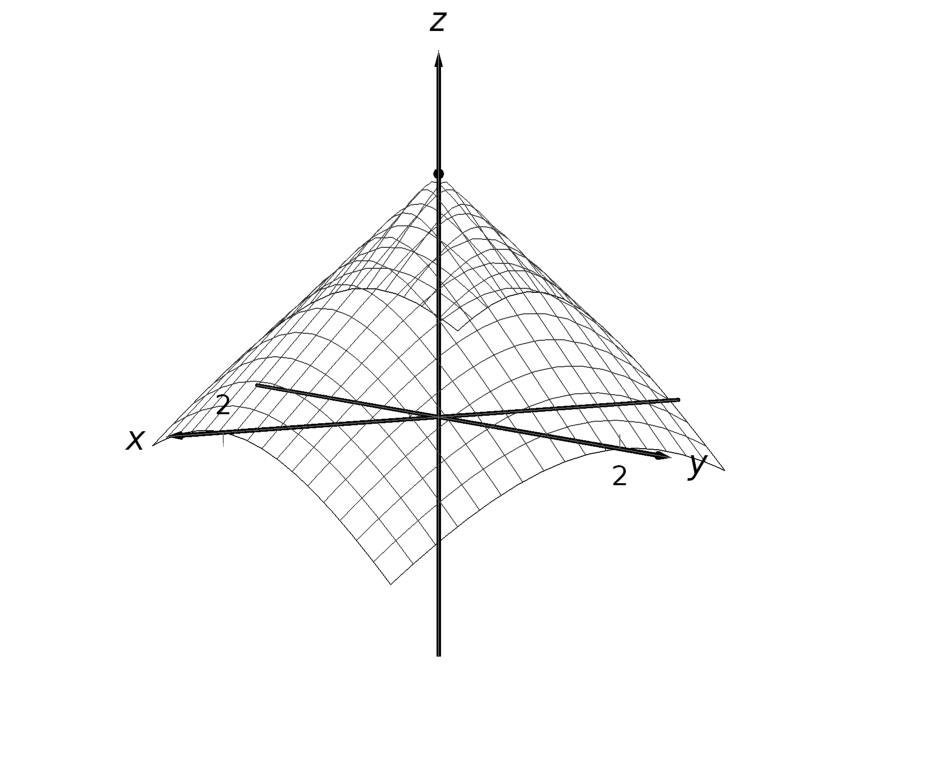
\includegraphics[width=0.4\textwidth]{fig_multi_var_24}
	\caption{The surface in Example \ref{ex_multi_extreme2} with its absolute maximum indicated.}
	\label{fig_multi_var_24}
	\end{center}
\end{figure}

\xhrulefill{gray}{2.5pt}Solution \xhrulefill{gray}{2.5pt}

We start by computing the partial derivatives of $f$:
$$f_x(x,y) = \frac{-x}{\sqrt{x^2+y^2}}\qquad \text{and}\qquad f_y(x,y) = \frac{-y}{\sqrt{x^2+y^2}}.$$
It is clear that $f_x=0$ when $x=0$ and $y\neq0$, and that $f_y=0$ when $y=0$ and $x\neq0$. At $(0,0)$, both $f_x$ and $f_y$ are not $0$, but  undefined. The point $(0,0)$ is hence a singular point, though.  The graph in Figure~\ref{fig_multi_var_24} shows that this point is the absolute maximum of $f$.
\end{example}


In this example we found a critical point of $f$ and then determined whether or not it was a local (or global) maximum or minimum by graphing. It would be nice to be able to determine whether a critical point corresponded to a max or a min without a graph. Before we develop such a test, we do two more examples that shed more light on the issues our test needs to consider.

\begin{example}\label{ex_multi_extreme3}
Let $f(x,y) = x^3-3x-y^2+4y$. Find the relative extrema of $f$.

\xhrulefill{gray}{2.5pt}Solution \xhrulefill{gray}{2.5pt}

Once again we start by finding the partial derivatives of $f$:
$$f_x(x,y) = 3x^2-3\qquad \text{and} \qquad f_y(x,y) = -2y+4.$$
Each is always defined. Setting each equal to 0 and solving for $x$ and $y$, we find
\begin{align*}
f_x(x,y) = 0 \quad & \Leftrightarrow \quad x = \pm 1\,,\\
f_y(x,y) = 0 \quad & \Leftrightarrow \quad y = 2.
\end{align*}
We have two critical points: $(-1,2)$ and $(1,2)$, while there are no singular points. To determine if they correspond to a relative maximum or minimum, we consider the graph of $f$ in Figure \ref{fig_multi_var_25}.


The critical point $(-1,2)$ clearly corresponds to a relative maximum. However, the critical point at $(1,2)$ is neither a maximum nor a minimum, displaying a different, interesting characteristic. 

If one walks parallel to the $y$-axis towards this critical point, then this point becomes a relative maximum along this path. But if one walks towards this point parallel to the $x$-axis, this point becomes a relative minimum along this path. A point that seems to act as both a maximum and a minimum is a saddle point. A formal definition follows.

\begin{figure}[H]
	\begin{center}
			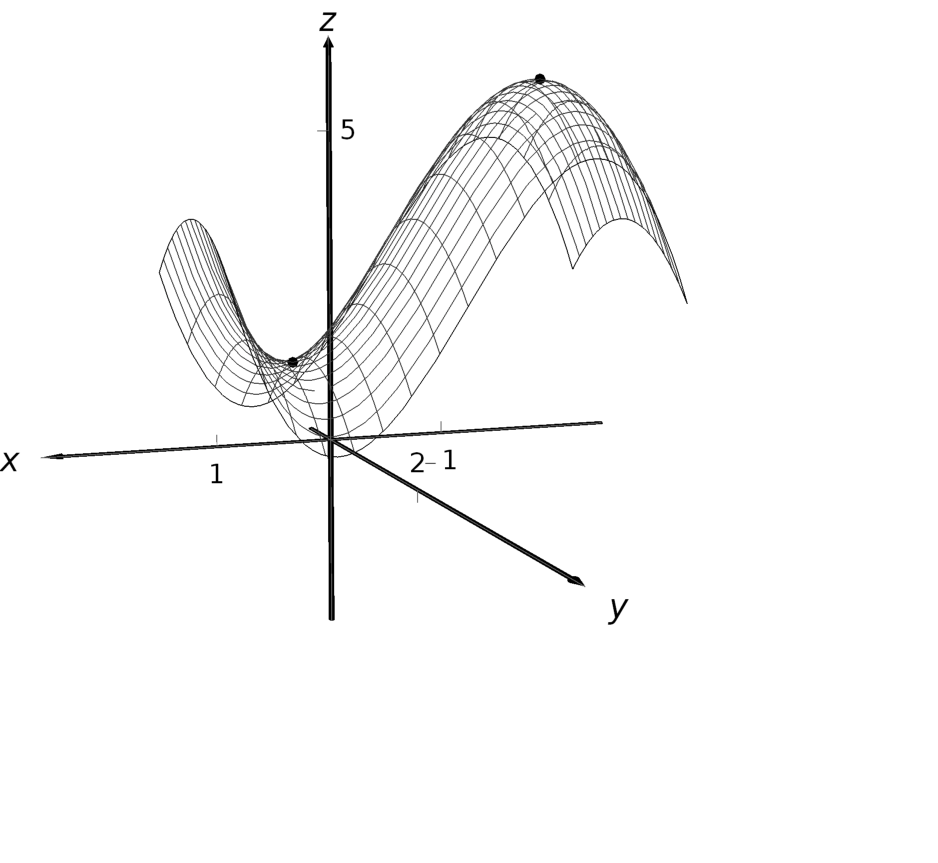
\includegraphics[width=0.5\textwidth]{fig_multi_var_25}
	\caption{The surface in Example \ref{ex_multi_extreme3} with both critical points marked.}
	\label{fig_multi_var_25}
	\end{center}
\end{figure}
\end{example}

\begin{definition}[Saddle  point]\label{def:saddle_point}
Let $P=(x_0,y_0)$ be in the domain of $f$ where $f_x=0$ and $f_y=0$ at $P$. We say $P$ is a \textbf{saddle point} (\textit{zadelpunt}) of $f$ if, for every open disk $D$ containing $P$, there are points $(x_1,y_1)$ and $(x_2,y_2)$ in $D$ such that $f(x_0,y_0)>f(x_1,y_1)$ and $f(x_0,y_0)<f(x_2,y_2)$.
\index{saddle point}\index{critical point}\index[aut]{zadelpunt}
\end{definition}

At a saddle point, the instantaneous rate of change in all directions is 0 and there are points nearby with $z$-values both less than and greater than the $z$-value of the saddle point.

\begin{example}
\label{FCP4}
Let us try to classify the critical points of $f(x,y) = 2 x^3 - 6 x y + 3 y^2$. As in the previous examples we start by setting the partial derivatives of $f$ to zero, resulting in the following nonlinear system: 

\begin{eqnarray*}
f_x(x,y) &=& 6 x^2 - 6 y = 0\,,\\ 
f_y(x,y) &=& -6 x + 6 y = 0\,.
\end{eqnarray*}
These partial derivatives are defined everywhere, so we have no singular points. To analyze the critical points, let us first put $f_y$ to zero, which yields $x=y$. Setting $f_x$ to zero and utilizing this observation then gives
$$6x^2 - 6x = 0 \qquad 
\Leftrightarrow \qquad 6x(x-1) = 0 \,. $$
As a result, $x$ must be $0$ or $1$. In both cases we also find a solution for $y$ when putting $f_y$ to zero. We obtain in this way two critical points: $(0,0)$ and $(1,1)$. 

Let us start by analyzing the point $(0,0)$. If this point is a minimum, then the value of the function has to increase when we move away from $(0,0)$ with a small step, irrespective of the direction. Similarly, if the point is a maximum, then the function must decrease if we move in any direction. So, let us assume that we move to the point $(h,k)$ from $(0,0)$ and let us analyze the difference in function values.     
$$
\Delta f = f(h,k) - f(0,0) =   2 h^3 - 6 hk + 3 k^2
$$
This difference $\Delta f$ does not have a fixed sign. It is sometimes negative, e.g.\ for $(h=-0.1,k=0)$, and sometimes positive, e.g.\ for $(h=0,k=0.1)$. So the point $(0,0)$ can neither be a local maximum, nor a local minimum. The point is a saddle point because the function increases when we move in a certain direction, while it decreases when we move in another direction. 

In a similar way let us analyze the point $(1,1)$. Again, we analyze the difference between the function in $(1,1)$ and a point close to $(1,1)$, namely the point $(1+h,1+k)$ in which $h$ and $k$ take positive or negative values that are close to zero (both values have to be close to zero because we are investigating local extrema, so we want to analyze the neighborhood of a critical point). A few manipulations will yield the following:  
\begin{eqnarray*}
 \Delta f &=& f(1+h,1+k) - f(1,1) \\ 
&=& 2 (1+h)^3 - 6 (1+h)(1+k) + 3 (1+k)^2 - (-1) \\
&=& \cdots \\
&=& 3 (h-k)^2 + h^2 (3+2h). \\ 
\end{eqnarray*}
For $h$ and $k$ close to zero this $\Delta f$ has a fixed sign. The first term is a square, and hence always positive. The second term is positive when $3+2h > 0$, so when $h > -3/2$. $\Delta f$ is always positive for $h$ and $k$ close to zero, so $f(1+h,1+k) \geq f(1,1)$ in that case.  We are sure that $(1,1)$ is a local minimum. Figure~\ref{fig_multi_var_26} plots the function $f$, and one can see that $(1,1)$ indeed is a point where $f$ reaches a local minimum. 

\begin{figure}[H]
\centering
%\raisebox{0.5cm}{
\subfigure[\label{fig_multi_var_26a}]{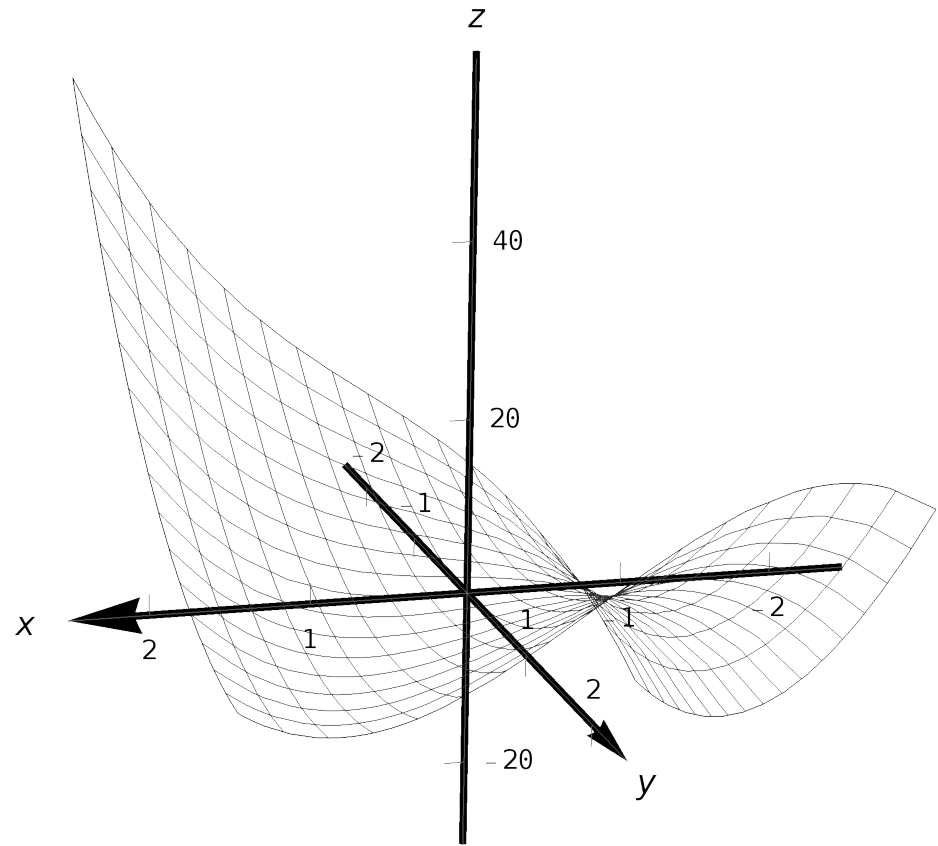
\includegraphics[width=0.43\textwidth]{fig_multi_var_26a}}
\qquad
\subfigure[\label{fig_multi_var_26b}]{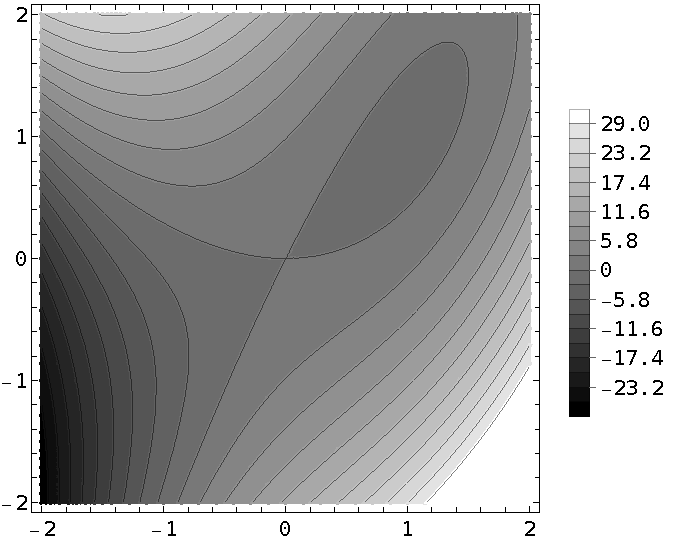
\includegraphics[width=0.43\textwidth]{fig_multi_var_26b}}
\caption{A plot of the function $f(x,y) = 2 x^3 - 6 x y + 3 y^2$:  graph of $z=f(x,y)$ (a) and  level curves (b).  \label{fig_multi_var_26}}
\end{figure}
\end{example} 


\subsection{Sufficient conditions for extrema}
\label{FMV}

\subsubsection{Functions of two variables}


Before Example \ref{ex_multi_extreme3} we mentioned the need for a test to differentiate between relative maxima and minima. We now recognize that our test also needs to account for saddle points. To do so, we consider the second partial derivatives of $f$. Recall that with single variable functions, such as $y=f(x)$, if $\fp'(c)>0$, then if $f$ is concave up at $c$, and if $\fp(c) =0$, then $f$ has a relative minimum at $x=c$.  Note that at a saddle point, it seems the graph is both concave up and concave down, depending on which direction you are considering.

It would be nice if the following were true:
\begin{center}
	\begin{tabular}{ccl}
	$f_{xx}\,\,\,$ and $\,\,\,f_{yy} >0$ & $\Rightarrow$ & relative minimum,\\
	$f_{xx}\,\,\,$ and $\,\,\,f_{yy} <0$ & $\Rightarrow$ & relative maximum,\\
	$f_{xx}\,\,\,$ and $\,\,\,f_{yy}$ have opposite signs & $\Rightarrow$ & saddle point.
	\end{tabular}
\end{center}

However, this is not the case. Functions $f$ exist where $f_{xx}$ and $f_{yy}$ are both positive  but a saddle point still exists. In such a case, while the concavity in the $x$-direction is up (i.e., $f_{xx}>0$) and the concavity in the $y$-direction is also up (i.e., $f_{yy}>0$), the concavity switches somewhere in between the $x$- and $y$-directions.



In Example~\ref{FCP4} we presented a simple procedure to determine whether a critical point corresponds to a local minimum, local maximum or a saddle point. This procedure was rather ad-hoc, because some arithmatic manipulations were needed to bring $\Delta f$ in a shape, so that we could analyze whether $\Delta f$ has a fixed sign. In addition to being ad-hoc, the procedure is also not very scalable, because the complexity of those manipulations increases when moving to functions of three \ifanalysis or more \fi variables. We will need a more systematic test to classify critical points. Remember from Theorem~\ref{NCFE} that we need to investigate for that purpose the critical points, singular points and end points of the domain. To analyze the critical and singular points, the gradient  $\vec{\nabla} f$ has to be analyzed and we have to set both partial derivatives to zero, which leads to a system of two equations. The solutions of this system will be the critical points, which will need further investigation. It is at this stage that so-called Hessian matrices come into play.

\begin{definition}[Hessian Matrix (of a function of two variables)]
\label{HM}
Suppose that $z=f(x,y)$ is a function that is twice differentiable w.r.t.\ all variables $x$ and $y$ Then, \textbf{the Hessian matrix $\mathscr{H}(x,y)$} (\textit{Hessiaan (matrix)}) of $f$ in the point $(x,y)$ is defined as
$$ \mathscr{H}(x,y) =
\begin{bmatrix}  f_{xx}(x,y) & f_{xy}(x,y) \\  f_{yx}(x,y) &   f_{yy}(x,y) \end{bmatrix} \,. $$
\end{definition} 
\index{Hessian}
\index[aut]{Hessiaan}

This Hessian matrix is the foundation for the so-called second derivative test that allows to classify critical points.

\begin{theorem}[Second derivative test]
\label{SDT}
Suppose that $P=(x_0,y_0) \in \mathbb{R}^2$ is a critical point of the function $f(x,y)$ and lying in the interior of the domain of $f$. Also, suppose that all  the second partial derivatives are continuous throughout a neighborhood of $P$ so that the Hessian matrix is also continuous in that neighborhood.
\begin{enumerate}
\item If $\mathscr{H}(x_0,y_0)$ is positive definite, then $f$ has a local minimum at $P$;
\item If $\mathscr{H}(x_0,y_0)$ is negative definite, then $f$ has a local maximum  at $P$;
\item If $\mathscr{H}(x_0,y_0)$ is indefinite, then $f$ has a saddle point at $P$;
\item If $\mathscr{H}(x_0,y_0)$ is neither positive definite, nor negative definite, nor indefinite, then this test gives no information. 
\end{enumerate}
\end{theorem}
 Note that the continuity of the partials guarantees that $\mathscr{H}(x_0,y_0)$ is a symmetric matrix. 
 
 Clearly, it is crucial to know the nature of $\mathscr{H}(x_0,y_0)$ in terms of it definiteness. Fortunately, we can rely on the following theorem for this purpose. 
 
 \begin{theorem}[Definiteness of symmetric matrices]
 \label{CQFUD}
Let $A$ be a real, symmetric $m \times m$ matrix. Let us consider the sequence $D_1,D_2,...,D_m$ of determinants defined by
$$D_1 = \begin{vmatrix} a_{11} \end{vmatrix} \,, \quad  D_2 = \begin{vmatrix} a_{11} & a_{12}  \\ a_{21} & a_{22} \end{vmatrix} \,, \quad  D_i = \begin{vmatrix} a_{11} & \ldots & a_{1i} \\ \vdots& &\vdots \\ a_{i1} & \ldots &  a_{ii} \end{vmatrix} \,,$$ 
where $1 \leq i \leq m$. Then the following hold:
\begin{itemize}
\item If $D_i > 0$ for $1 \leq i \leq m$, then $A$ is positive definite;
\item If $D_i > 0$ for all even $i$ and $D_i < 0$ for all odd $i$, then $A$ is negative definite;
\item If $D_m = \det(A) \neq 0$ and the above situations do not apply, then $A$ is indefinite; 
\item If $D_m = \det(A) = 0$, then $A$ is positive or negative semi-definite.  
\end{itemize}
\end{theorem}

 
 We now first practice using this test with some of the functions in the previous examples, where we visually determined whether a critical point corresponded to a local minimum, local maximum or saddle point. 
 
 \begin{example}
 \label{USDT}
Let $f(x,y) = x^3-3x-y^2+4y$ be as in Example~\ref{ex_multi_extreme3} and let us investigate whether the function has a local minimum, local maximum, or saddle point at each critical point.
We determined previously that the critical points of $f$ are $(-1,2)$ and $(1,2)$. To use the second derivative test, we must find the second partial derivatives of $f$:
$$f_{xx}(x,y) = 6x,\qquad f_{yy}(x,y) = -2,\qquad f_{xy}(x,y) = 0.$$
Organizing them in the Hessian matrix gives
\begin{eqnarray*}
\mathscr{H}(x,y) &=&  \begin{bmatrix} 6x & \quad 0 \\  0 & -2  \end{bmatrix} \,.
\end{eqnarray*}
For the critical point $(-1,2)$ one obtains the following matrix:
\begin{eqnarray*}
 \mathscr{H}(-1,2) &=& \begin{bmatrix} -6 & 0 \\ 0 & -2  \end{bmatrix} \,.
\end{eqnarray*}
Applying Theorem~\ref{CQFUD} gives $D_1 = -6 < 0$ and $D_2 = 12 >0$, so the matrix is negative definite and we have a local maximum. 
For the critical point $(1,2)$ one obtains 
\begin{eqnarray*} 
\mathscr{H}(1,2) &=& \begin{bmatrix} 6 & 0 \\ 0 & -2  \end{bmatrix} \,.
\end{eqnarray*}
Applying Theorem~\ref{CQFUD} gives in this case $D_1 = 6>0$ and $D_2 = -12 < 0$, so the matrix is indefinite and we have a saddle point. 
The second derivative test confirmed what we determined visually.
\end{example}

\begin{example}
\label{USDT2}
Let $f(x,y) = 2 x^3 - 6 x y + 3 y^2$ be as in Example~\ref{FCP4}. We found two critical points $(0,0)$ and $(1,1)$. Let us first construct the Hessian matrix for an arbitrary point $(x,y)$.
\begin{eqnarray*}
\mathscr{H}(x,y) &=& \begin{bmatrix} f_{xx}(x,y) & \quad f_{xy}(x,y) \\ f_{yx}(x,y) & \quad f_{yy}(x,y)  \end{bmatrix} =  \begin{bmatrix} 12x & \quad -6 \\  -6 & 6  \end{bmatrix}
\end{eqnarray*}
For the critical point $(0,0)$ one obtains the following matrix:
\begin{eqnarray*}
 \mathscr{H}(0,0) &=& \begin{bmatrix} 0 & -6 \\ -6 & 6  \end{bmatrix} \,.
\end{eqnarray*}
Applying Theorem~\ref{CQFUD} gives $D_1= 0$ and $D_2=-36 \neq 0$, so the matrix is indefinite and we have a saddle point. 
For the critical point $(1,1)$ one obtains 
\begin{eqnarray*} 
\mathscr{H}(1,1) &=& \begin{bmatrix} 12 & -6 \\ -6 & 6  \end{bmatrix}  \,.
\end{eqnarray*}
Applying Theorem~\ref{CQFUD} gives in this case $D_1=12>0$ and $D_2=36>0$, so the matrix is positive definite and we have a local minimum. 
\end{example}


\subsubsection{Functions of three variables}
To determine the extrema of a function of three variables $w=f(x,y,z)$, we proceed in the same way as before upon intuitively extending Theorem~\ref{NCFE} the definition of the Hessian to such functions.

\begin{definition}[Hessian Matrix (of a function of three variables)]
\label{HM3}
Suppose that $w=f(x,y,z)$ is a function that is twice differentiable w.r.t.\ all variables $x$, $y$ and $z$. Then, \textbf{the Hessian matrix $\mathscr{H}(x,y,z)$} (\textit{Hessiaan (matrix)}) of $f$ in the point $(x,y,z)$ is defined as
$$ \mathscr{H}(x,y,z) =
\begin{bmatrix}  f_{xx}(x,y,z) & f_{xy}(x,y,z) & f_{xz}(x,y,z) \\  f_{yx}(x,y,z) & f_{yy}(x,y,z)&  f_{yz}(x,y,z)\\
f_{zx}(x,y,z)&f_{zy}(x,y,z)&f_{zz}(x,y,z)\end{bmatrix} \,. $$
\end{definition} 
\index{Hessian}
\index[aut]{Hessiaan}

Combining this definition with the intuitive extension of Theorem~\ref{SDT} to functions of three variables allows us to classify the critical points of such functions. 

\begin{example}
\label{3V}
Determine the nature of the  extrema of $f(x,y,z) = x^2y + y^2z +z^2 -2x$. 

\xhrulefill{gray}{2.5pt}Solution \xhrulefill{gray}{2.5pt}

We start by computing the partial derivatives and equating them to zero, which results in the following system: 
\begin{eqnarray*}
f_x(x,y,z) &=& 2xy - 2=0\,, \\
f_y(x,y,z) &=& x^2 + 2yz=0\,, \\
f_z(x,y,z) &=& y^2 + 2z=0  \,. 
\end{eqnarray*}
From the third equation we learn that $z = -y^2 / 2$.  Substituting this in the second equation gives $ 
x^2 - y^3 = 0$. Substituting this last result in the first equation gives $y^{5/2}= 1$. As a result we have $y=1$ and we find one critical point $(1,1,-1/2)$. Let us compute the Hessian in that point: 
\begin{eqnarray*}
\mathscr{H}(x,y,z) = \begin{bmatrix} 
2y & 2x & 0 \\ 
2x & 2z  & 2y \\  
0 & 2y & 2
\end{bmatrix} & \mbox{and hence }&  
\mathscr{H}\left(1,1,-\frac{1}{2}\right) =  \begin{bmatrix} 
2 & 2 & 0 \\ 
2 & -1 & 2 \\
0 & 2 & 2
\end{bmatrix} \,. 
\end{eqnarray*}
Theorem~\ref{CQFUD} results in  $D_1 = 2$, $D_2 = -6$ and $D_3 = -20$. The matrix is indefinite, and the critical point is a saddle point. 
\end{example}

\section{Constrained optimisation}
\label{ERD}
In the previous chapter we have analyzed extrema of functions up to three variables without making any restrictions on the domain. In this section we further specialize in functions with a restricted domain. This portion of mathematics is often entitled \textbf{constrained optimization} (\textit{gebonden extremumproblemen}) because we want to optimize a function (i.e.\ find its maximum and/or minimum values) subject to a constraint -- some limit to what values the function can attain. 

Solving constrained optimization problems is a very important topic in applied mathematics, and we will discuss some applications in this chapter. In Section~\ref{CO} we first present some general techniques for finding extrema in a restricted domain, before discussing the specific but widely-applicable case of linear functions in Section~\ref{LP}.  We will mainly focus on functions of two variables to keep things simple, but the techniques developed here are the basis for solving larger problems, where more than two variables are involved.

\subsection{Extrema in a restricted domain}
\label{CO}
When optimizing functions of one variable such as $y=f(x)$, you made use of the extreme value theorem (Theorem~\ref{thm:extreme_val}), which said that over a closed interval $I$, a continuous function has both a maximum and minimum value.

A similar theorem applies to functions of several variables  over a closed set (see Definition~\ref{def:open}). We can find these values by evaluating the function at the critical and singular points in the set and over the boundary of the set. After formally stating this extreme value theorem for functions of three variables, we give examples.

\begin{theorem}[Extreme Value Theorem]
\label{EVT}
Let $w=f(x,y,z)$ be a continuous function defined on a closed, bounded set $S$. Then $f$ has a global maximum and minimum value on $S$.
\end{theorem}
\ifanalysis
A formal proof of the theorem is beyond the scope of this course. The next two examples will make it intuitively clear that the theorem must hold. 
\fi

\begin{example}
\label{FECS}
Let $f(x,y) = x^2-y^2+5$ and let $S$ be the triangle with vertices $(-1,-2)$, $(0,1)$ and $(2,-2)$. Determine the maximum and minimum values of $f$ on $S$.

\xhrulefill{gray}{2.5pt}Solution \xhrulefill{gray}{2.5pt}

It can help to see a graph of $f$ along with the set $S$. In Figure \ref{fig_multi_var_27a} the triangle defining $S$ is shown on the surface of $f$, as we are only concerned with the portion of $f$ enclosed by the triangle on its surface. 


\begin{figure}[H]
\centering
%\raisebox{0.5cm}{
\subfigure[\label{fig_multi_var_27a}]{\includegraphics[width=0.43\textwidth]{fig_multi_var_27a}}
\qquad
\subfigure[\label{fig_multi_var_27b}]{\includegraphics[width=0.43\textwidth]{fig_multi_var_27b}}
\caption{Plot of the surface of $f$ in Example~\ref{FECS} (a), along with the restricted domain $S$ (b). \label{fig_multi_var_27}}
\end{figure}


We begin by finding the critical points of $f$. With $f_x = 2x$ and $f_y = -2y$, we find only one critical point, at $(0,0)$, which is situated in $S$. 

We now find the maximum and minimum values that $f$ attains along the boundary of $S$, that is, along the edges of the triangle. In Figure \ref{fig_multi_var_27b} we see the triangle sketched in the plane with the equations of the lines forming its edges labeled. Start with the bottom edge, along the line $y=-2$. If $y=-2$, then on the surface, we are considering points $f(x,-2)$; that is, our function reduces to $f(x,-2) = x^2-(-2)^2+5 = x^2+1=f_1(x)$. We want to maximize/minimize $f_1(x)=x^2+1$ on the interval $[-1,2]$. To do so, we evaluate $f_1(x)$ at its critical points and at the endpoints. The critical points of $f_1$ are found by setting its derivative equal to 0:
$$f_1'(x)= 2x = 0\qquad \Leftrightarrow \qquad x=0.$$
Evaluating $f_1$ at this critical point, and at the endpoints of $[-1,2]$ gives:
\begin{align*}
f_1(-1) = 2 \qquad&\Rightarrow\qquad f(-1,-2) = 2,\\
f_1(0) = 1 \qquad&\Rightarrow \qquad f(0,-2) = 1,\\
f_1(2) = 5 \qquad&\Rightarrow \qquad f(2,-2) = 5.
\end{align*}
Notice how evaluating $f_1$ at a point is the same as evaluating $f$ at its corresponding point.

We need to do this process twice more, for the other two edges of the triangle. Along the left edge, along the line $y=3x+1$, we substitute $3x+1$ in for $y$ in $f(x,y)$:
$$f(x,y) = f(x,3x+1) = x^2-(3x+1)^2+5 = -8x^2-6x+4 = f_2(x).$$
We want the maximum and minimum values of $f_2$ on the interval $[-1,0]$, so we evaluate $f_2$ at its critical points and the endpoints of the interval. We find the critical points:
$$f_2'(x) = -16x-6=0 \qquad \Leftrightarrow \qquad x=-3/8.$$
Evaluate $f_2$ at its critical point and the endpoints of $[-1,0]$:
\begin{align*}
f_2(-1) = 2 \qquad&\Rightarrow\qquad f(-1,-2) = 2,\\
f_2(-3/8) = 5.125  \qquad&\Rightarrow \qquad f(-3/8,-1/8) = 5.125,\\
f_2(0) = 1 \qquad&\Rightarrow \qquad f(0,1) = 4.
\end{align*}
Finally, we evaluate $f$ along the right edge of the triangle, where $y = -\frac{3}{2}x+1$. 
$$f(x,y) = f\left(x,-\frac{3}{2}x+1\right) = x^2-\left(-\frac{3}{2}x+1\right)^2+5 = -\frac54x^2+3x+4=f_3(x).$$
The critical points of $f_3(x)$ are:
$$f_3'(x) = -\frac{5}{2} x+3 = 0 \qquad \Leftrightarrow \qquad x=\frac{6}{5}=1.2.$$
We evaluate $f_3$ at this critical point and at the endpoints of the interval $[0,2]$:
\begin{align*}
f_3(0) = 4 \qquad&\Rightarrow\qquad f(0,1) = 4,\\
f_3(1.2) = 5.8  \qquad&\Rightarrow \qquad f(1.2,-0.8) = 5.8,\\
f_3(2) = 5 \qquad&\Rightarrow \qquad f(2,-2) = 5.
\end{align*}
One last point to test: the critical point of $f$, $(0,0)$. We find $f(0,0) = 5$.


We have evaluated $f$ at a total of 7 different places. We checked each vertex of the triangle twice, as each showed up as the endpoint of an interval twice. Of all the $z$-values found, the maximum is 5.8, found at $(1.2,-0.8)$; the minimum is 1, found at $(0,-2)$. 
\end{example}


We illustrate the technique once more with a classic problem that also emphasizes the practical usefulness of constrained optimization.  

\begin{example}
 Post NL states that the girth pluslength of a standard post package must not exceed 130. Given a rectangular box, the length is the longest side, and the so-called girth is twice the width+height. Given a rectangular box where the width and height are equal, what are the dimensions of the box that give the maximum volume subject to the constraint of the size of a standard post package?

\xhrulefill{gray}{2.5pt}Solution \xhrulefill{gray}{2.5pt}


Let $w$, $h$ and $\ell$ denote the width, height and length of a rectangular box; we assume here that $w=h$. The girth is then $2(w+h) = 4w$. The volume of the box is $V(w,\ell) = wh\ell = w^2\ell$. We want to maximize this volume subject to the constraint $4w+\ell\leq 130$, or $\ell\leq 130-4w$. Common sense also indicates that $\ell \geq 0, w \geq 0$. Moreover, for $\ell = 0$ or $w  = 0$ one cannot obtain a maximum, so this part of the boundary does not need further investigation. 

We begin by finding the critical values of $V$. We find that $V_w = 2w\ell$ and $V_\ell = w^2$; these are simultaneously 0 only at $(0,0)$. This gives a volume of 0, so we can ignore this critical point. 

We now consider the volume along the constraint $\ell=130-4w.$ Along this line, we have:
$$V(w,\ell) = V(w,130-4w) = w^2(130-4w) = 130w^2-4w^3 = V_1(w).$$
The constraint is applicable on the $w$-interval $[0,130/4]$ as indicated in the figure. Thus we want to maximize $V_1$ on $[0,32.5]$. Finding the critical values of $V_1$, we take the derivative and set it equal to 0:
$$V'_1(w) = 260w-12w^2 = 0 \quad \Leftrightarrow \quad w(260-12w)= 0 \quad \Leftrightarrow \quad w=0 \vee\,\frac{260}{12}\approx 21.67.$$
We found two critical values: when $w=0$ and when $w=21.67$. We again ignore the $w=0$ solution, because then $V=0$. The maximum volume, subject to the constraint, comes at $w=h=21.67$, $\ell = 130-4(21.67) =43.33.$ This gives a volume of $V(21.67,43.33) \approx 20.343$in$^3$. 

The volume function $V(w,\ell)$ is shown in Figure \ref{fig_multi_var_28} along with the constraint $\ell = 130-4w$. As done previously, the constraint is drawn dashed in the $xy$-plane and also along the surface of the function. The point where the volume is maximized is indicated.

\begin{figure}[H]
\centering
\includegraphics[width=0.43\textwidth]{fig_multi_var_28}
\caption{Graphing the volume of a box with girth $4w$ and length $\ell$, subject to a size constraint.}
\label{fig_multi_var_28}
\end{figure}


\end{example}

In the previous two examples we have deployed the same procedure to find the global maximum and minimum in a restricted domain. In essence this procedure consists of three steps. 
\begin{enumerate}
\item Find any critical or singular points in the interior of the domain $S$.
\item Find any points on the boundary of $S$ where $f$ might have extreme values. To do so, you can parameterize the whole boundary, or parts of it, and express $f$ as a function of the parameters. If you break the boundary into pieces, you must analyze the end points of those pieces. 
\item Evaluate $f$ on all the points found in steps 1 and 2. 
\end{enumerate}


\subsection{Linear programming}
\label{LP}
It is hard to overemphasize the importance of optimization. In ``the real world'', we routinely seek to make something better. By expressing the something as a mathematical function, ``making something better'' means ``optimize some function''.  In this section we further specialize in methods to achieve the best outcome (such as maximum profit or lowest cost) in a mathematical model whose requirements are represented by linear relationships. 

More formally, linear programming is a technique for the optimization of a linear objective function, subject to linear equality and linear inequality constraints. Its feasible region is a convex polytope, which is a special type of convex set, defined by one or several linear inequalities. Its objective function is a real-valued linear function defined on this convex polytope. A linear programming algorithm finds a point in the convex polytope where this function has the smallest (or largest) value if such a point exists. Linear programs are problems that can be expressed in canonical form as
$${\displaystyle {\begin{aligned}&{\text{Maximize}}&&\vec{c}^T \vec{x}, \\&{\text{subject to}}&&A\vec{x} \leq \vec {b}, \\&{\text{and}}&&\vec{x} \geq \vec{0}. \end{aligned}}}$$
where $\vec{x}$ represents the vector of variables (to be determined), $\vec{c}$ and $\vec{b}$ are vectors of (known) coefficients, $A$ is a (known) matrix of coefficients. The expression to be maximized or minimized is called the objective function ($\vec{c}^T \vec{x}$ in this case). The inequalities $A\vec{x} \leq \vec {b}$ and $\vec{x} \geq \vec{0}$ are the constraints which specify a convex polytope over which the objective function is to be optimized. In this context, two vectors are comparable when they have the same dimensions. If every entry in the first is less-than or equal-to the corresponding entry in the second, then it can be said that the first vector is less-than or equal-to the second vector.

Linear programming can be applied to various fields of study. It is widely used in mathematics, and to a lesser extent in business, economics, and for some engineering problems. Industries that use linear programming models include transportation, energy, telecommunications, and manufacturing. It has proven useful in modeling diverse types of problems in planning, routing, scheduling, assignment, and design. 


\begin{example}
\label{LP_ex_1}
A store has requested a manufacturer to produce pants and sports jackets. For materials, the manufacturer has 750 $m^2$ of cotton textile and 1000 $m^2$ of polyester. Every pair of pants (1 unit) needs $1 m^2$ of cotton and 2 $m^2$ of polyester. Every jacket needs $1.5 m^2$ of cotton and 1 $m^2$ of polyester. The price of the pants is fixed at \euro 50 and the jacket at  \euro 40. What is the number of pants and jackets that the manufacturer must give to the stores so that these items obtain a maximum sale?


\xhrulefill{gray}{2.5pt}Solution \xhrulefill{gray}{2.5pt}


 To solve this problem, let us start with defining the unknowns. 
\begin{eqnarray*}
x &=& \mbox{number of pants} \\
y &=& \mbox{number of jackets}
\end{eqnarray*}
In the second step the objective function needs to be constructed. The manufacturer wants to have a maximum sale, so the following objective needs to be maximized. 

$$f(x,y)= 50x + 40y$$

We have to maximize this function subject to a number of constraints. With the unknowns that we have defined, those constraints become
\begin{eqnarray*}
x + 1.5y &\leq& 750\,, \\
2x + y &\leq& 1000 \,.
\end{eqnarray*}
Simplifying the first constraints, and observing that the number of pants and jackets are natural numbers, we end up with the following set of four constraints: 
\begin{eqnarray*}
 2x+3y &\leq& 1500\,, \\
2x + y &\leq& 1000\,, \\
x &\geq& 0\,, \\
y &\geq& 0 \,.
\end{eqnarray*}
Those four constraints define the restricted domain of $f$, in which a maximum needs to be found. 

In the next step, let us represent the restricted domain in a two-dimensional graph.  As $x \geq 0$ and $y \geq 0$, we work in the first quadrant. Next, we plot the other two constraints as straight lines by replacing the inequality by an equality. To draw these lines, determine their points of intersection with the axes, as shown in Figure~\ref{fig_multi_var_29}. Together the four constraints define a feasible region that represents the restricted domain of the function $f$. 

\begin{figure}[H]
\centering
\includegraphics[width=0.5\textwidth]{fig_multi_var_29}
\caption{A plot of the restricted domain of the objective function in Example~\ref{LP_ex_1}. The lines correspond to the constraints of the linear program, and the grey region represents the feasible region.}
\label{fig_multi_var_29}
\end{figure}

To find the maximum, we have to analyze the interior and the boundary of this restricted domain. The objective function $f$ is a linear function, and its gradient is the vector $$\vec{\nabla} f(x,y) = \begin{bmatrix}50 \\ 40\end{bmatrix} \,.$$ Hence the function $f$ does not have any critical points or singular points in the interior. 

It suffices to analyze the boundary, and the gradient can give us useful information on which part of the boundary needs further investigation. In this case the gradient points in a direction that makes more or less an angle of $\pi/4$ with the horizontal axis. The optimal solution, if unique, must be in a vertex, and the origin can be excluded because $f(0,0) =0$.  We therefore analyze the other three vertices of the feasible region. These are the solutions to the systems:
\begin{eqnarray*}
2x + 3y = 1500; x = 0          & \quad \Rightarrow \quad &(x,y)= (0, 500) \\
2x + y = 1000; y = 0           & \quad \Rightarrow \quad &(x,y)= (500, 0)\\
2x + 3y =1500;\,  2x + y = 1000   &\quad \Rightarrow \quad &(x,y)= (375, 250)
\end{eqnarray*}
We have to calculate the value of the objective function at each of the vertices to determine which of them has the maximum or minimum values. The possible non-existence of a solution must be taken into account, if the compound is not bounded:
\begin{eqnarray*}
f(0, 500) &=& 50\times0 + 40\times500 = \text{\euro }\,20000, \\
f(500, 0) &=& 50\times500 + 40\times0 = \text{\euro }\,25000, \\
f(375, 250) &=& 50\times375 + 40\times250 = \text{\euro }\,28750. 
\end{eqnarray*}
The optimum solution is to make 375 pants and 250 jackets to obtain a benefit of \euro $28750$.
\end{example}

Let us remark that in the previous example we did not make use of vectors notations, as we were analyzing a linear program in two variables. In vector notation the objective function $\vec{c}^T \vec{x}$ would have been the vectors $$\vec{c} = \begin{bmatrix}50 \\ 40\end{bmatrix} \qquad  \mbox{and} \qquad  \vec{x} = \begin{bmatrix}x \\ y\end{bmatrix} \,. $$ 
The first two constraints could be written as $A \vec{x} \leq \vec{b}$ with 
$$A = \begin{bmatrix} 2 & 3 \\ 2 & 1 \end{bmatrix} \qquad  \mbox{and} \qquad  \vec{b} = \begin{bmatrix} 1500 \\ 1000 \end{bmatrix} \,.$$
The last two constraints could simply be written as $\vec{x} \geq 0$.   

The previous example has provided a couple of interesting properties of linear programs. When the objective function is linear, no critical points or singular points can occur in the interior of the feasible region, because the gradient will always differ from zero. In linear programs it will suffice to analyze the boundary, and because the feasible region is a convex polytope, this analysis will also be straightforward. For linear programs in two or three variables one can often determine the maxima visually. For more than three variables, there exist computer algorithms that find the maxima efficiently. A method called the simplex algorithm is commonly used. In this course we will only consider pen-and-paper techniques for objective functions with two or three variables. 

In the previous example a unique solution was found. However, the solution is not always unique, as shown in the next and final example. 

\pagebreak
\begin{example}
\label{LP_ex_2}
If the objective function of Example~\ref{LP_ex_1} is modified to
$$f(x,y) = 20x + 30y \,,$$
then we find
\begin{eqnarray*}
f(0,500) &=& 20\times 0 + 30 \times 500 = \text{\euro} 15000 \\
f(500, 0) &=& 20 \times 500 + 30 \times 0 = \text{\euro} 10000 \\
f(375, 250) &=& 20 \times 375 + 30 \times 250 = \text{\euro} 15000 
\end{eqnarray*}
In this case, we will find more than one maximum. The objective function will have a maximum at all $(x,y)$ points with integer solutions on the segment that connects $(0,500)$ and $(375,250)$. This line segment is drawn with dashes Figure~\ref{fig_multi_var_30}. 


\begin{figure}[H]
\centering
\includegraphics[width=0.5\textwidth]{fig_multi_var_30}
\caption{A plot of the restricted domain of the objective function in Example~\ref{LP_ex_2}. In this case the maximum is not unique. The objective function has a maximum at value at all points on the black line.}
\label{fig_multi_var_30}
\end{figure}


So, when exactly will a linear program have more than one solution? Observe that for this modified objective function the gradient is $$\vec{\nabla} f(x,y) = \begin{bmatrix}20 \\ 30 \end{bmatrix} \,.$$
The gradient points in a direction orthogonal to the dashed line segment. The line segment coincides with a level curve of the function $f$. 
\end{example}

More generally, if a part of the boundary coincides with a level curve of the objective function, then a linear program can have more than one solution. Moreover, because the objective is linear, the level curves will always be straight lines. In economics these lines are also known as iso-profit lines. 


\fi

\ifanalysis

\section{Extreme values}
\label{ERD}
Given a function $z=f(x,y)$, we are often interested in points where $z$ takes on the largest or smallest values. For instance, if $z$ represents a cost function, we would likely want to know what $(x,y)$ values minimize the cost. If $z$ represents the ratio of a volume to surface area, we would likely want to know where $z$ is greatest. This leads to the following definition.

\begin{definition}[Relative and absolute extreme]\label{def:multi_extrema}
Let $z=f(x,y)$ be defined on a set $S$ containing the point $P=(x_0,y_0)$.
\begin{enumerate}
	\item	If $f(x_0,y_0)\geq f(x,y)$ for all $(x,y)$ in $S$, then $f$ has an \textbf{absolute maximum} (\textit{globaal maximum}) at $P$.
	
	If $f(x_0,y_0)\leq f(x,y)$ for all $(x,y)$ in $S$, then $f$ has an \textbf{absolute minimum} (\textit{globaal minimum}) at $P$.
	
	\item If there is an open disk $D$ containing $P$ such that $f(x_0,y_0) \geq f(x,y)$ for all points $(x,y)$ that are in both $D$ and $S$, then $f$ has a \textbf{relative maximum} (\textit{lokaal maximum}) at $P$.
	
	If there is an open disk $D$ containing $P$ such that $f(x_0,y_0) \leq f(x,y)$ for all points $(x,y)$ that are in both $D$ and $S$, then $f$ has a \textbf{relative minimum} (\textit{lokaal minimum}) at $P$.
	
	
	\item		If $f$ has an absolute maximum or minimum at $P$, then $f$ has an \textbf{absolute extrema} at $P$.
	
	If $f$ has a relative maximum or minimum at $P$, then $f$ has a \textbf{relative extrema} at $P$.
	
	
\end{enumerate}
\index{function ! (absolute) maximum}\index[aut]{functie ! (absoluut) maximum}
\index{function ! (absolute) minimum}\index[aut]{functie ! (absoluut) minimum}
\index{extreme values}\index[aut]{extreme waarden}
\index{absolute maximum}\index[aut]{absoluut maximum}
\index{absolute minimum}\index[aut]{absoluut minimum}
\index{maximum}\index[aut]{maximum}
\index{minimum}\index[aut]{minimum}
\index{extrema}\index[aut]{extrema}
\end{definition}

If $f$ has a relative or absolute maximum at $P=(x_0,y_0)$, it means that every curve on the surface of $f$ through $P$ will also have a relative or absolute maximum at $P$. Recalling what we learned in Section \ref{sec:extreme_values}, the slopes of the tangent lines to these curves at $P$ must be 0 or undefined. Since directional derivatives are computed using $f_x$ and $f_y$, we are led to the following definition and theorem.

\begin{definition}[Critical point]\label{def:multi_critical_point}
Let $z = f(x,y)$ be continuous on a set $S$. A \textbf{critical point} (\textit{kritisch punt}) $P=(x_0,y_0)$ of $f$ is a point in $S$ such that, at $P$,\index{critical point}\index[aut]{kritisch punt}
$$
f_x(x_0,y_0) = 0 \text{ and } f_y(x_0,y_0) = 0
$$
\end{definition}

Besides, when $f_x(x_0,y_0)$ and/or $f_y(x_0,y_0)$ is undefined, we call $P=(x_0,y_0)$ a \textbf{singular point}, just as we did within the framework of functions of one variable (Definition~\ref{def:singularnum}). \index{singular point}

\begin{theorem}[Critical and singular points and relative extrema]\label{thm:multi_critical_point}
Let $z=f(x,y)$ be defined on an open set $S$ containing $P=(x_0,y_0)$. If $f$ has a relative extrema at $P$, then $P$ is a critical or singular point of $f$.\index{extrema!relative}\index{critical point}
\end{theorem}

Therefore, to find relative extrema, we find the critical and singular points of $f$ and determine which correspond to relative maxima, relative minima, or neither. The following examples demonstrates this.

\begin{example}\label{ex_multi_extreme2}
Let $f(x,y) = -\sqrt{x^2+y^2}+2$. Find the relative extrema of $f$. The surface of $f$ is graphed in Figure \ref{fig_multi_var_22} along with the point $(0,0,2)$.

\begin{figure}[H]
	\begin{center}
			\includegraphics[width=0.4\textwidth]{fig_multi_var_24}
	\caption{The surface in Example \ref{ex_multi_extreme2} with its absolute maximum indicated.}
	\label{fig_multi_var_22}
	\end{center}
\end{figure}

\xhrulefill{gray}{2.5pt}Solution \xhrulefill{gray}{2.5pt}

We start by computing the partial derivatives of $f$:
$$f_x(x,y) = \frac{-x}{\sqrt{x^2+y^2}}\qquad \text{and}\qquad f_y(x,y) = \frac{-y}{\sqrt{x^2+y^2}}.$$
It is clear that $f_x=0$ when $x=0$ and $y\neq0$, and that $f_y=0$ when $y=0$ and $x\neq0$. At $(0,0)$, both $f_x$ and $f_y$ are not $0$, but rather undefined. The point $(0,0)$ is hence a singular point, though.  The graph in Figure~\ref{fig_multi_var_22} shows that this point is the absolute maximum of $f$.
\end{example}





\begin{example}\label{ex_multi_extreme3}
Let $f(x,y) = x^3-3x-y^2+4y$. Find the relative extrema of $f$.

\pagebreak
\xhrulefill{gray}{2.5pt}Solution \xhrulefill{gray}{2.5pt}

Once again we start by finding the partial derivatives of $f$:
$$f_x(x,y) = 3x^2-3\qquad \text{and} \qquad f_y(x,y) = -2y+4.$$
Each is always defined. Setting each equal to 0 and solving for $x$ and $y$, we find
\begin{align*}
f_x(x,y) = 0 \quad & \Rightarrow \quad x = \pm 1\\
f_y(x,y) = 0 \quad & \Rightarrow \quad y = 2.
\end{align*}
We have two critical points: $(-1,2)$ and $(1,2)$, while there are no singular points. To determine if they correspond to a relative maximum or minimum, we consider the graph of $f$ in Figure \ref{fig_multi_var_23}.


The critical point $(-1,2)$ clearly corresponds to a relative maximum. However, the critical point at $(1,2)$ is neither a maximum nor a minimum, displaying a different, interesting characteristic. 

If one walks parallel to the $y$-axis towards this critical point, then this point becomes a relative maximum along this path. But if one walks towards this point parallel to the $x$-axis, this point becomes a relative minimum along this path. A point that seems to act as both a maximum and a minimum is a saddle point. A formal definition follows.

\begin{figure}[H]
	\begin{center}
			\includegraphics[width=0.5\textwidth]{fig_multi_var_25}
	\caption{The surface in Example \ref{ex_multi_extreme3} with both critical points marked.}
	\label{fig_multi_var_23}
	\end{center}
\end{figure}
\end{example}

\begin{definition}[Saddle  point]\label{def:saddle_point}
Let $P=(x_0,y_0)$ be in the domain of $f$ where $f_x=0$ and $f_y=0$ at $P$. We say $P$ is a \textbf{saddle point} (\textit{zadelpunt}) of $f$ if, for every open disk $D$ containing $P$, there are points $(x_1,y_1)$ and $(x_2,y_2)$ in $D$ such that $f(x_0,y_0)>f(x_1,y_1)$ and $f(x_0,y_0)<f(x_2,y_2)$.
\index{saddle point}\index{critical point}\index[aut]{zadelpunt}
\end{definition}

At a saddle point, the instantaneous rate of change in all directions is 0 and there are points nearby with $z$-values both less than and greater than the $z$-value of the saddle point.

Before Example \ref{ex_multi_extreme3} we mentioned the need for a test to differentiate between relative maxima and minima. We now recognize that our test also needs to account for saddle points. To do so, we consider the second partial derivatives of $f$. Recall that with single variable functions, such as $y=f(x)$, if $\fp'(c)>0$, then if $f$ is concave up at $c$, and if $\fp(c) =0$, then $f$ has a relative minimum at $x=c$.  Note that at a saddle point, it seems the graph is both concave up and concave down, depending on which direction you are considering.

It would be nice if the following were true:
\begin{center}
	\begin{tabular}{ccl}
	$f_{xx}\,\,\,$ and $\,\,\,f_{yy} >0$ & $\Rightarrow$ & relative minimum,\\
	$f_{xx}\,\,\,$ and $\,\,\,f_{yy} <0$ & $\Rightarrow$ & relative maximum,\\
	$f_{xx}\,\,\,$ and $\,\,\,f_{yy}$ have opposite signs & $\Rightarrow$ & saddle point.
	\end{tabular}
\end{center}

However, this is not the case. Functions $f$ exist where $f_{xx}$ and $f_{yy}$ are both positive  but a saddle point still exists. In such a case, while the concavity in the $x$-direction is up (i.e., $f_{xx}>0$) and the concavity in the $y$-direction is also up (i.e., $f_{yy}>0$), the concavity switches somewhere in between the $x$- and $y$-directions.

To account for this, consider 
$$D = f_{xx}f_{yy} \, - \, f_{xy}f_{yx}.$$
 Since $f_{xy}$ and $f_{yx}$ are equal when continuous (refer back to Theorem \ref{thm:mixed_partial}), we can rewrite this as $D = f_{xx}f_{yy}-f_{xy}^{\,2}$. $D$ can be used to test whether the concavity at a point changes depending on direction. If $D>0$, the concavity does not switch (i.e., at that point, the graph is concave up or down in all directions). If $D<0$, the concavity does switch. If $D=0$, our test fails to determine whether concavity switches or not. We state the use of $D$ in the following theorem.

\begin{theorem}[Second derivative test]\label{thm:multi_second_test}
Let $R$ be an open set on which a function $z=f(x,y)$ and all its first and second partial derivatives are defined, let $P = (x_0,y_0)$ be a critical point of $f$ in $R$, and let 
\index{Second Derivative Test}\index{maximum!relative/local}\index{minimum!relative/local}\index{saddle point}
$$D(x_0,y_0) = f_{xx}(x_0,y_0)f_{yy}(x_0,y_0)-f_{xy}^{\,2}(x_0,y_0).$$
\begin{enumerate}
	\item If $D>0$ and $f_{xx}(x_0,y_0)>0$, then $f$ has a relative minimum at $P$.
	\item If $D>0$ and $f_{xx}(x_0,y_0)<0$, then $f$ has a relative maximum at $P$.
	\item	If $D<0$, then $f$ has a saddle point at $P$.
	\item If $D=0$, the test is inconclusive.
\end{enumerate}
\end{theorem}

We practice this test with the function in the previous example, where we visually determined we had a relative maximum and a saddle point.\\
%\clearpage

\begin{example}\label{ex_multi_extreme4}
Let $f(x,y) = x^3-3x-y^2+4y$ as in Example \ref{ex_multi_extreme3}. Determine whether the function has a relative minimum, maximum, or saddle point at each critical point.


\xhrulefill{gray}{2.5pt}Solution \xhrulefill{gray}{2.5pt}

We determined previously that the critical points of $f$ are $(-1,2)$ and $(1,2)$. To use the second derivative test, we must find the second partial derivatives of $f$:
$$f_{xx} = 6x;\qquad f_{yy} = -2;\qquad f_{xy} = 0.$$
Thus $D(x,y) = -12x$. 

At $(-1,2)$: $D(-1,2) = 12>0$, and $f_{xx}(-1,2) = -6$. By the second derivative test, $f$ has a relative maximum at $(-1,2)$.

At $(1,2)$: $D(1,2) = -12 <0$. The second derivative test states that $f$ has a saddle point at $(1,2)$.

The second derivative test confirmed what we determined visually.
\end{example}


\fi

	\begin{center}
			\includegraphics[width=0.65\textwidth]{GreatMath_6.jpg}
	\end{center}
 
\newpage
\section{Exercices}
\renewcommand{\ExerciseListName}{Assignement}

\subsection*{\nameref{sec:multi_intro}}
%%%%%%%%%%%%%%%%
%Exercise 1
%%%%%%%%%%%%%%%%
\begin{Exercise} Find the domain and image of the functions below.
\begin{multicols}{2}
	\ifcalculus
	\Question[difficulty=1] $f(x,y) = \dfrac{1}{\sqrt{4-x^2-y^2}}$ 
	\fi
	\Question[difficulty=1] $f(x,y)=\dfrac{\ln (x)}{\sin (y)}$
	\Question[difficulty=3] $f(x,y)=\dfrac{2+\arcsin (y)}{\ln (2x)}$
	\ifanalysis\Question[difficulty=1]\fi\ifcalculus\Question[difficulty=2]\fi  $f(x,y) = \sqrt{1-x^2-y^2}$
	\ifanalysis\Question[difficulty=1]\fi\ifcalculus\Question[difficulty=2]\fi $f(x,y) = \sin (xy)$
	\ifanalysis\Question[difficulty=2]\fi\ifcalculus\Question[difficulty=3]\fi $f(x,y) = |x| - |y|$
	\Question[difficulty=1] $f(x,y)=\dfrac{1}{x-y}$
	\ifanalysis\Question[difficulty=2]\fi\ifcalculus\Question[difficulty=3]\fi $f(x,y) = \ln^{-1} (x^2 + y^2 - 3)$
	\ifanalysis\Question[difficulty=2]\fi\ifcalculus\Question[difficulty=3]\fi $f(x,y)=\pi - \arcsin (x^2 + 2y^2)$
    \EndCurrentQuestion
\end{multicols}
\end{Exercise}

\setboolean{firstanswerofthechapter}{true}
\begin{Answer}
    
    \Question $\dom\, f = \left\{ (x,y) | \ x^2 + y^2 < 4 \right\}$ \quad and \quad $\im\, f =  \mathbb{R}_0^+$ %Uit Van Hecke H2, vb 2.1

    \Question $\dom\, f = \left\{ (x,y) | \ x \in \mathbb{R}^+_0 \; \wedge \; y \in \mathbb{R} \backslash \{k \pi, k \in \mathbb{Z} \}\right\}$ \quad and \quad $\im\, f = \mathbb{R}$
    \Question $\dom\, f = \left\{ (x,y) | \ x \in \mathbb{R}^+\backslash \left\{0,1/2\right\} \; \wedge \; y \in [-1,1]\right\}$ \quad and \quad $\im\, f = \mathbb{R}_0$
    \Question $\dom\, f = \left\{ (x,y) | \ x^2 + y^2 \leq 1 \right\}$ \quad and \quad $\im\, f = [0,1]$
    \Question $\dom\, f = \left\{ (x,y) | \ x \in \mathbb{R}\; \wedge \; y \in \mathbb{R} \right\}$ \quad and \quad $\im\, f = [-1,1]$
    \Question $\dom\, f = \left\{ (x,y) | \ x \in \mathbb{R}\; \wedge \; y \in \mathbb{R} \right\}$ \quad and \quad $\im\, f = \mathbb{R}$
    \Question $\dom\, f = \left\{ (x,y) | \ x \neq y \right\}$ \quad and \quad $\im\, f = \mathbb{R}_0$
    \Question $\dom\, f = \left\{ (x,y) | \ x^2 + y^2 > 3; \wedge \; x^2 + y^2 \neq 4 \right\}$ \quad and \quad $\im\, f = \mathbb{R}_0$
    \Question $\dom\, f = \left\{ (x,y) |  \ x^2 + 2y^2 \leq 1 \right\}$ \quad and \quad $\im\, f = \left[ \dfrac{\pi}{2}, \pi \right]$
    
\end{Answer}
\setboolean{firstanswerofthechapter}{false}

%%%%%%%%%%%%%%%%
%Oefening 2
%%%%%%%%%%%%%%%%
\begin{Exercise} Sketch some level curves for the functions below
\begin{multicols}{2}
		\Question[difficulty=1] $f(x,y)=\dfrac{x^2}{y}$ 
		\ifanalysis\Question[difficulty=2]\fi\ifcalculus\Question[difficulty=3]\fi $f(x,y) = \dfrac{y}{x^2+y^2}$ 
		\Question[difficulty=2] $f(x,y)=\sqrt{\dfrac{1}{y}-x^2}$ 
        \EndCurrentQuestion
\end{multicols}
\end{Exercise}

\begin{Answer}
    
        \Question The level curves corresponding to $c \neq 0$ are parabolas with their vertex at the origin and the $y$-axis as axis of symmetry. The level curves corresponding to $c=0$ is  al ine (the $y$-axis). 
        \Question The level curves corresponding to $c \neq 0$ are circles with the center at the $y$-axis. The level curves corresponding to $c=0$ are lines (the $x$-axis). 
        \Question The level curves corresponding to $c \neq 0$ are bell-shaped curves with the $y$-axis as the axis of symmetry. The level curve for $c=0$ is a curve with the $y$-axis as its vertical asymptote. 
\end{Answer}


%%%%%%%%%%%%%%%%
%Oefening 3 Bio-irs
%%%%%%%%%%%%%%%%
\ifanalysis
\begin{Exercise}[difficulty = 3, label=oef_niveaukrommes] In each case, describe the graph of the function $f(x,y)$ whose level curves $f(x,y)=C$ are represented in Figure \ref{fig_mult_var_31} (a) and (b). 
\begin{figure}[H]
\includegraphics[scale=0.4]{fig_mult_var_31a} \hspace{1.5cm}
\includegraphics[scale=0.4]{fig_mult_var_31b}
\caption{Level curves $f(x,y) = C$ of the function $f(x,y)$ from Exercise 3. }
\label{fig_mult_var_31}
\end{figure}

\end{Exercise}

\begin{Answer}
    
        \Question The circles in figure (a) all have the origin as their center. The circle with radius $5$ corresponds to $C=0$, the origin to $C=5$. The relationship between the radius $r$ of the circles and the constant $C$ is $r+C=5$. The circles are given by $x^2+y^2 = (5-C)^2$. Therefore, we conclude that $C=5-\sqrt{x^2+y^2} \ (C \leq 5)$. The level curves are derived from the surface $z=f(x,y)=5-\sqrt{x^2+y^2}$. This is a semicircular cone with top in $(0,0,5)$.
        \Question The lines in figure (b) are not equidistant. We see that $C=10$ corresponds to $y=5$ and $C=0$ with $y=-5$. The relationship between $C$ and $y$ is $C-y=5$. Therefore we conclude that $C=y+5$. The level curves are derived from the surface $z=f(x,y)=\sqrt{y+5}$. This is a parabolic cylinder parallel to the $x$-axis.
    
\end{Answer}

\pagebreak\fi
\subsection*{\nameref{sec:partial_derivatives}}
\ifanalysis
%%%%%%%%%%%%%%%%
%Oefening 4 Bio-irs
%%%%%%%%%%%%%%%%
\begin{Exercise}[difficulty = 2] Find $f_x(0,0)$ and $f_y(0,0)$ for the functions below, if they exist, by using definition: \ref{def:partial_derivative}. 
\[ f(x,y) = \left\{\begin{array}{ll} (x^3+y) \sin \left(\dfrac{1}{x^2+y^2} \right), \quad & \quad \text{ if } (x,y) \neq (0,0), \\
0, &\quad \text{ if } (x,y) = (0,0). \end{array} \right. \]
Find $f_x(x,y)$. Is it continuous in $(0,0)$?
\end{Exercise}

\begin{Answer}

    $f_x(0,0) = \ds \lim_{h \to 0} \dfrac{1}{h} \left(h^3 \sin \left( \dfrac{1}{h^2} \right)  \right) = 0$\\[0.2cm]
    $f_y(0,0) = \ds \lim_{k \to 0} \dfrac{1}{k} \left(k \sin \left( \dfrac{1}{k^2} \right)  \right)$ does not exist \\[0.2cm]
    $f_x(x,y) = 3 x^2 \sin \left( \dfrac{1}{x^2+y^2} \right) - \dfrac{(x^3+y)2x}{\left(x^2+y^2\right)^2} \cos\left( \dfrac{1}{x^2+y^2} \right)$ \\[0.2cm]
    $\ds \lim_{(x,y)\to (0,0)} f_x(x,y)$ does not exist, thus $f_x(x,y)$ is not continuous in $(0,0)$.
\end{Answer}

\fi

%%%%%%%%%%%%%%%%
%Extra oefening Ings
%%%%%%%%%%%%%%%%
\ifcalculus
\begin{Exercise} Calculate the first-order partial derivatives of the functions below.
%\begin{multicols}{2}
    \Question[difficulty=1] $f(x,y) = x^2+2y^2-3x+2y+3$
    \Question[difficulty=1] $f(x,y) = 2x^3y^2+2y+4x$
    \Question[difficulty=1] $f(x,y) = \sin\left(2x^3-y^3\right)$
    \Question[difficulty=2] $f(x,y) = e^{x^2}\cos(xy)$
    \Question[difficulty=2] $f(x,y) = y\sin\left(x^2+y^2\right)$
    \Question[difficulty=2] $f(x,y) = x^4\sin\left(xy^3\right)$
    \Question[difficulty=2] $f(x,y) = e^{xy}\sin\left(4y^2\right)$
    \Question[difficulty=2] $f(x,y) = \dfrac{x+y}{x-y}$
    \Question[difficulty=3] $f(x,y) = y^{-3/2}\arctan\left(\dfrac{x}{y}\right)$
    \Question[difficulty=1] $f(x,y) = \sqrt{x^2+4y^2}$
    \Question[difficulty=1] $f(x,y,z) = x^2-2y^2+3z^2+4xy+5xz+6yz$
    \Question[difficulty=1] $f(x,y,z) = x^2y^4z^3+xy+z^2+1$
    \Question[difficulty=1] $f(x,y,z) = \sqrt{x^2+y^2+z^2}$
    \Question[difficulty=1] $f(x,y,z) = x^2y\cos(z)$
    \Question[difficulty=2] $f(x,y,z) = z^2\ln(x^2y)$
%\end{multicols}
\end{Exercise}

\begin{Answer}

    \Question $f_x = 2x-3$\qquad and \qquad $f_y = 4y+2$ 
    \Question $f_x = 6x^2y^2+4$\qquad and\qquad $f_y = 4x^3y+2$ 
    \Question $f_x = 6x^2\cos\left(2x^3-y^3\right)$\qquad and\qquad $f_y = -3y^2 \cos\left(2x^3-y^3\right)$ 
    \Question $f_x = e^{x^2}\left(2x\cos(xy)-y\sin(xy)\right)$\qquad and\qquad $f_y = -x\,e^{x^2}\sin(xy)$ 
    \Question  $f_x = 2xy\cos\left(x^2+y^2\right)$\qquad and\qquad $f_y = \sin\left(x^2+y^2\right) + 2y^2 \cos\left(x^2+y^2\right)$ 
    \Question $f_x = 4x^3\sin\left(xy^3\right) + x^4y^3\cos\left(xy^3\right) $\qquad and\qquad $f_y = 3x^5y^2\cos\left(xy^3\right)$  
    \Question $f_x = y\,e^{xy}\sin\left(4y^2\right)$\qquad en\qquad $f_y = x\,e^{xy}\sin\left(4y^2\right) + 8y\,e^{xy}\cos\left(4y^2\right)$ 
    \Question $f_x = -\dfrac{2y}{(x-y)^2}$\qquad and\qquad $f_y = \dfrac{2x}{(x-y)^2}$ 
    \Question $f_x = \dfrac{1}{\sqrt{y}\left(x^2+y^2\right)}$\qquad and\qquad $f_y = -\dfrac{x}{y^{3/2} \left(x^2 + y^2\right)} - \dfrac{3}{2}y^{-5/2} \arctan\left(\dfrac{x}{y}\right)$ 
    \Question $f_x = \dfrac{x}{\sqrt{x^2+4y^2}} $\qquad and\qquad $f_y = \dfrac{4y}{\sqrt{x^2+4y^2}}$ 
    
    \Question  $f_x = 2x+4y+5z$\qquad and\qquad $f_y = -4y+4x+6z$\qquad and\qquad $f_z = 6z+5x+6y$ 
    \Question $f_x = 2xy^4z^3+y$\qquad and\qquad $f_y = 4x^2y^3z^3+x $\qquad and\qquad $f_z = 3x^2y^4z^2+2z$  
    \Question $f_x = \dfrac{x}{\sqrt{x^2+y^2+z^2}}$\qquad and\qquad $f_y = \dfrac{y}{\sqrt{x^2+y^2+z^2}}$\qquad and\qquad $f_z = \dfrac{z}{\sqrt{x^2+y^2+z^2}}$  
    \Question $f_x = 2xy\cos(z)$\qquad and\qquad $f_y = x^2\cos(z) $\qquad and\qquad $f_z = -x^2y\sin(z)$  
    \Question $f_x = \dfrac{2z^2}{x}$\qquad and\qquad $f_y = \dfrac{z^2}{y}$\qquad and\qquad $f_z = 2z\ln(x^2y)$  
    
\end{Answer}
\fi





%%%%%%%%%%%%%%%%
%Oefening 6 Bio-irs
%Oefening 4 Ings
%%%%%%%%%%%%%%%%
\begin{Exercise} Find the partial derivatives of the first and second order of the functions below, and at the specified point. \label{part_afg_3_verand}
	\Question[difficulty=2] $f(x,y,z) = \arctan ( x + y + z ) \hfill  (1,0,0) \hspace{2cm}$
	\Question[difficulty=1] $f(x,y,z) = x^2 + 3 y^2 + 6 z^2 - 2 x y + 6 x z + 7 y z + 4 x - 3 y + 7\hfill  (0,0,0)\hspace{2cm}$
	\ifanalysis\Question[difficulty=1]\fi\ifcalculus\Question[difficulty=2]\fi $f(x,y,z) = \sqrt{xy+z^2} \hfill  (1,1,1)\hspace{2cm}$
	\ifanalysis\Question[difficulty=2]\fi\ifcalculus\Question[difficulty=3]\fi $f(x,y,z) = x e^{xy+z} \hfill  (1,0,0)\hspace{2cm}$
	\Question[difficulty=2] $f(x,y,z) = e^{x+y^2+z^3} \hfill  (0,0,0)\hspace{2cm}$
	\Question[difficulty=2] $f(x,y,z) = x\sin (y) + y\ln (z) \hfill  (1,\pi,1)\hspace{2cm}$
	\Question[difficulty=3] $f(x,y,z) = (xy)^z + z^{xy} \hfill  (1,1,1)\hspace{2cm}$
\end{Exercise}

\begin{Answer}\\
    \vspace{-0.65cm}
    $\renewcommand{\arraystretch}{1.5}\begin{array}{|c|c|c|c|c|c|c|}
    &&&&&&\vspace{-0.77cm}\\
    \hline
    &&&&&&\vspace{-0.6cm}\\
    & f_x & \mbox{in } a  & f_y & \mbox{in } a & f_z & \mbox{in } a   \\
    &&&&&&\vspace{-0.65cm}\\
    \hline
    &&&&&&\vspace{-0.55cm}\\
    \mbox{(a)} & \dfrac{1}{1+(x+y+z)^2} & \dfrac{1}{2} & \dfrac{1}{1+(x+y+z)^2} & \dfrac{1}{2}  & \dfrac{1}{1+(x+y+z)^2} & \dfrac{1}{2} \\[0.25cm]
    \hline
    \mbox{(b)} & 2x-2y+6z+4 & 4 & 6y-2x+7z-3 & -3  & 12z+6x+7y & 0  \\ 
    \hline
    &&&&&&\vspace{-0.55cm}\\
    \mbox{(c)} & \dfrac{y}{2\sqrt{xy+z^2}} & \dfrac{\sqrt{2}}{4} & \dfrac{x}{2\sqrt{xy+z^2}} & \dfrac{\sqrt{2}}{4}   & \dfrac{z}{\sqrt{xy+z^2}} & \dfrac{\sqrt{2}}{2}  \\[0.35cm] 
    \hline
    \mbox{(d)} & \left(1+xy\right)e^{xy+z} & 1 & x^2\,e^{xy+z} & 1  & x\, e^{xy+z} & 1  \\
    \hline
    \mbox{(e)} & e^{x+y^2+z^3} & 1 & 2y\,e^{x+y^2+z^3} & 0  & 3z^2\,e^{x+y^2+z^3} & 0  \\ 
    \hline
    &&&&&&\vspace{-0.55cm}\\
    \mbox{(f)} & \sin (y) & 0 & x\cos (y) + \ln (z) & -1 & \dfrac{y}{z} & \pi  \\[0.25cm] 
    \hline
    &&&&&&\vspace{-0.55cm}\\
    \mbox{(g)} & \mbox{\begin{small}$\dfrac{(xy)^z\,z}{x}+z^{xy}\,y\ln (z)$\end{small}} & 1 & \mbox{\begin{small}$\dfrac{(xy)^z\,z}{y}+z^{xy}\,x\ln (z)$\end{small}} & 1 & \mbox{\begin{small}$(xy)^z\ln (xy) + \dfrac{z^{xy}\,xy}{z}$\end{small}} & 1  \vspace{-0.5cm} \\
    &&&&&&\vspace{-0.07cm}\\
    \hline
    \end{array}$
    
    \npar
    
    $\renewcommand{\arraystretch}{1.5}\begin{array}{|c|c|c|c|c|c|c|}
    &&&&&&\vspace{-0.77cm}\\
    \hline
    &&&&&&\vspace{-0.6cm}\\
    & f_{xx} & \mbox{in } a & f_{xy} & \mbox{in } a & f_{yy} & \mbox{in } a\\
    &&&&&&\vspace{-0.65cm}\\
    \hline
    &&&&&&\vspace{-0.55cm}\\
    \mbox{(a)} & \mbox{\begin{footnotesize}$-\dfrac{2(x+y+z)}{(1+(x+y+z)^2)^2}$\end{footnotesize}} & -\dfrac{1}{2} & =f_{xx} & -\dfrac{1}{2} & =f_{xx} & -\dfrac{1}{2} \\[0.25cm]
    \hline
    \mbox{(b)} & 2 & 2 & -2 & -2 & 6 & 6  \\ 
    \hline
    &&&&&&\vspace{-0.65cm}\\
    \mbox{(c)} & -\dfrac{y^2}{4(xy+z^2)^\frac{3}{2}} & -\dfrac{\sqrt{2}}{16} & \dfrac{xy+2z^2}{4(xy+z^2)^\frac{3}{2}} & \dfrac{3\sqrt{2}}{16} & -\dfrac{x^2}{4(xy+z^2)^\frac{3}{2}} & -\dfrac{\sqrt{2}}{16} \\[0.35cm]
    \hline
    \mbox{(d)} & y e^{xy+z}\left(xy+2\right) & 0 & \mbox{\begin{small}$x e^{xy+z}\left(xy+2\right)$\end{small}} & 2 & x^3e^{xy+z} & 1  \\ 
    \hline
    \mbox{(e)} & e^{x+y^2+z^3} & 1 & 2y e^{x+y^2+z^3} & 0 & \mbox{\begin{small}$2\left(2y^2+1\right)e^{x+y^2+z^3}$\end{small}} & 2  \\ 
    \hline
    \mbox{(f)} & 0 & 0 & \cos (y) & -1 & -x\sin (y) & 0  \\
    \hline
    \mbox{(g)} & \mbox{(*)} & 0 & \mbox{(*)} & 1 & \mbox{(*)} & 0 \vspace{-0.7cm} \\ 
    &&&&&&\vspace{-0.07cm}\\
    \hline
    \end{array}$
    \npar
    \mbox{(*)}: These expressions are too long to fit in the table
    \npar
    $\renewcommand{\arraystretch}{1.5}\begin{array}{|c|c|c|c|c|c|c|}
    &&&&&&\vspace{-0.77cm}\\
    \hline
    &&&&&&\vspace{-0.6cm}\\
    & f_{xz} & \mbox{in } a & f_{yz} & \mbox{in } a & f_{zz} & \mbox{in } a\\
    &&&&&&\vspace{-0.65cm}\\
    \hline
    &&&&&&\vspace{-0.55cm}\\
    \mbox{(a)} & =f_{xx} & -\dfrac{1}{2} & =f_{xx} & -\dfrac{1}{2} & =f_{xx} & -\dfrac{1}{2} \\[0.25cm]
    \hline
    \mbox{(b)} & 6 & 6 & 7 & 7 & 12 & 12  \\ 
    \hline
    &&&&&&\vspace{-0.65cm}\\
    \mbox{(c)} & -\dfrac{yz}{2(xy+z^2)^\frac{3}{2}} & -\dfrac{\sqrt{2}}{8} & -\dfrac{xz}{2(xy+z^2)^\frac{3}{2}} & -\dfrac{\sqrt{2}}{8} & \dfrac{xy}{(xy+z^2)^\frac{3}{2}} & \dfrac{\sqrt{2}}{4} \\[0.35cm]
    \hline
    \mbox{(d)} & e^{xy+z}\left(xy+1\right) & 1 & x^2 e^{xy+z} & 1 & x e^{xy+z} & 1  \\ 
    \hline
    \mbox{(e)} & 3z^2e^{x+y^2+z^3} & 0 & 6yz^2 e^{x+y^2+z^3} & 0 & 3z\left(3z^3+2\right)e^{x+y^2+z^3} & 0  \\ 
    \hline
    &&&&&&\vspace{-0.55cm}\\
    \mbox{(f)} & 0 & 0 & \dfrac{1}{z} & 1 & -\dfrac{y}{z^2} & -\pi  \\[0.25cm] 
    \hline
    \mbox{(g)} & \mbox{(*)} & 2 & \mbox{(*)} & 2 & \mbox{(*)} & 0 \vspace{-0.7cm}
     \\ 
    &&&&&&\vspace{-0.07cm}\\
    \hline
    \end{array}$
    \npar
    \mbox{(*)}: These expressions are too long to fit in the table
\end{Answer}


%%%%%%%%%%%%%%%%%
%Extra oefening Ings
%Uit Van Hecke H11 oef 2(a, b, d)
%%%%%%%%%%%%%%%%%
\ifcalculus
\begin{Exercise} Determine what's requested.
    \Question[difficulty=1] $\dfrac{\partial z}{\partial x}$ \quad if \ $z = e^{xy(x^2+y^2)}$
    \Question[difficulty=1] $\dfrac{\partial u}{\partial x}, \dfrac{\partial u}{\partial y}, \dfrac{\partial u}{\partial z}$ \quad if \  $u = 2y\sqrt{x} + 3y^2 \sqrt[3]{z^2}$
    \Question[difficulty=2] $dz$ \quad if \  $z = \arctan \left( \dfrac{x+y}{x-y} \right)$

\end{Exercise}

\begin{Answer}
    
    \Question $\dfrac{\partial z}{\partial x} = e^{xy(x^2+y^2)} (3x^2y + y^3)$
    \Question $\dfrac{\partial u}{\partial x} = \dfrac{y}{\sqrt{x}}, \quad  \dfrac{\partial u}{\partial y} = 2\sqrt{x} + 6y \sqrt[3]{z^2}, \quad \dfrac{\partial u}{\partial z} = \dfrac{2y^2}{\sqrt[3]{z}}$ 
    \Question $dz = \dfrac{x dy - y dx}{x^2 + y^2} $ 

\end{Answer}
\fi

%%%%%%%%%%%%%%%%
%Oefening 7 Bio-irs
%Oefening 5 Ings
%%%%%%%%%%%%%%%%
\ifanalysis\begin{Exercise}[difficulty = 1]\fi\ifcalculus\begin{Exercise}[difficulty = 2]\fi Let $z = \ln \left( \sqrt{x^2 + y^2} \right)\,.$ Then, prove $$x \, \dfrac{\partial z}{\partial x}+ y \, \dfrac{\partial z}{\partial y} = 1.$$  
\ifanalysis\end{Exercise}\fi\ifcalculus\end{Exercise}\fi

\begin{Answer}

    $\dfrac{\partial z}{\partial x} = \dfrac{x}{x^2 + y^2}, \quad  \dfrac{\partial z}{\partial y}= \dfrac{y}{x^2 + y^2} $
\end{Answer}

%\ifanalysis\pagebreak\fi
%%%%%%%%%%%%%%%%
%Oefening 8 Bio-irs
%Oefening 6 Ings
%%%%%%%%%%%%%%%%
\ifanalysis\begin{Exercise}[difficulty = 2]\fi\ifcalculus\begin{Exercise}[difficulty = 3]\fi Let
$$z = e^\frac{x}{y} \sin \left( \dfrac{x}{y} \right) + e^\frac{y}{x}\cos \left( \dfrac{y}{x} \right).$$
Then, prove
$$x \, \frac{\partial z}{\partial x} + y \, \frac{\partial z}{\partial y} = 0.$$  
\ifanalysis\end{Exercise}\fi\ifcalculus\end{Exercise}\fi

\begin{Answer}

    $\dfrac{\partial z}{ \partial x} = \dfrac{e^\frac{x}{y} }{y}\left(\sin \left( \dfrac{x}{y} \right) + \cos \left( \dfrac{x}{y} \right) \right) - \dfrac{ye^\frac{y}{x} }{x^2} \left(\cos \left( \dfrac{y}{x}\right)   - \sin\left(  \dfrac{y}{x}\right) \right)$\\[0.2cm] 
$\dfrac{\partial z}{ \partial y} = -\dfrac{xe^\frac{x}{y} }{y^2}\left(\sin\left(  \dfrac{x}{y} \right)  + \cos \left( \dfrac{x}{y}\right)  \right) + \dfrac{e^\frac{y}{x}}{x} \left(\cos \left(  \dfrac{y}{x} \right)  - \sin \left( \dfrac{y}{x}\right)  \right) $
\end{Answer}


\ifanalysis

%%%%%%%%%%%%%%%%
%Oefening 9 Bio-irs
%%%%%%%%%%%%%%%%
\begin{Exercise}[difficulty = 3] Prove that $z=f(x)g(y)$ satisfies
$$z\, \dfrac{\partial^2 z}{\partial x \partial y} = \dfrac{\partial z}{\partial x }\,  \dfrac{\partial z}{\partial y }. $$ 
\end{Exercise}

\begin{Answer}

    $\dfrac{\partial z}{\partial x } = f'(x)g(y), \quad  \dfrac{\partial z}{\partial y } = f(x)g'(y), \quad \dfrac{\partial^2 z}{\partial x \partial y} = f'(x)g'(y)$
\end{Answer}

\ifanalysis\pagebreak\fi
%%%%%%%%%%%%%%%%
%Oefening 10 Bio-irs
%%%%%%%%%%%%%%%%
\begin{Exercise}[difficulty = 3] Let $z = A\sin (a\lambda y+\varphi)\sin (\lambda x)$. Then, prove that
$$\dfrac{\partial^2 z}{\partial y^2}=a^2\dfrac{\partial^2 z}{\partial x^2}\cdot$$  
\end{Exercise}

\begin{Answer}
    $\dfrac{\partial^2 z}{\partial x^2} = -A \lambda^2 \sin \left(\lambda x \right)\sin (a\lambda y+\varphi), \quad \dfrac{\partial^2 z}{\partial y^2}= -a^2 A \lambda^2\sin \left(\lambda x \right)\sin (a\lambda y+\varphi)$
\end{Answer}

%%%%%%%%%%%%%%%%
%Oefening 11 Bio-irs
%%%%%%%%%%%%%%%%
\begin{Exercise}[difficulty = 2] Prove that the function $u(x,y,t) = t^{-1}\, e^{-(x^2+y^2)/(4t)}$ is a solution of the two-dimensional heat equation
\[ \dfrac{\partial u}{\partial t} = \dfrac{\partial^2 u}{\partial x^2} + \dfrac{\partial^2 u}{\partial y^2}. \]
\end{Exercise}

\begin{Answer}

    $\dfrac{\partial u}{ \partial t} = \dfrac{e^{-(x^2+y^2)/(4t)}}{t^2} \left( -1 + \dfrac{x^2+y^2}{4t} \right)$ \\[0.2cm]
 $\dfrac{\partial^2 u}{ \partial x^2} = \dfrac{e^{-(x^2+y^2)/(4t)}}{2t^2} \left( -1 + \dfrac{x^2}{2t} \right)$\\[0.2cm]
 $\dfrac{\partial^2 u}{ \partial y^2} = \dfrac{e^{-(x^2+y^2)/(4t)}}{2t^2} \left( -1 + \dfrac{y^2}{2t} \right)$
\end{Answer}

%%%%%%%%%%%%%%%%
%Oefening 12 Bio-irs
%%%%%%%%%%%%%%%%
\begin{Exercise}[difficulty = 2] Let$u=x^2y+y^2z+z^2x$. Then, prove  $$\dfrac{\partial u}{\partial x}+\dfrac{\partial u}{\partial y}+\dfrac{\partial u}{\partial z} = (x+y+z)^2.$$ 
\end{Exercise}

\begin{Answer}

    $\dfrac{\partial u}{ \partial x} = 2xy + z^2, \quad \dfrac{\partial u}{ \partial y} = x^2 + 2yz, \quad \dfrac{\partial u}{ \partial z} = y^2 + 2zx $
\end{Answer}

\fi

%%%%%%%%%%%%%%%%
%Extra oefening
%%%%%%%%%%%%%%%%
\begin{Exercise}[difficulty = 3] Consider the Van der Waals equation
\[ f(p,V,n,T) = \left( p+\dfrac{n^2a}{V^2}\right)(V-nb) - nRT = 0, \]
with $a, b$ and $R$ constant. Find
\begin{multicols}{2}
    \Question $\left(\dfrac{\partial V}{\partial T}\right)_{p,n}$
    \Question $\left(\dfrac{\partial V}{\partial p}\right)_{T,n}$
    \Question $\left(\dfrac{\partial p}{\partial T}\right)_{V,n}$
    \Question $\left(\dfrac{\partial p}{\partial V}\right)_{T,n}$
    \EndCurrentQuestion
\end{multicols}
The notation $\left(\dfrac{\partial f}{\partial x}\right)_{y,z}$ indicates that $y$ and $z$ are considered constants when differentiating with respect  to $x$.
\end{Exercise}

\begin{Answer}

    \Question $\left(\dfrac{\partial f}{\partial T}\right)_{p,n} = \left(-\dfrac{2n^2a}{V^3}\right) \left(\dfrac{\partial V}{\partial T}\right)_{p,n}(V-nb) + \left( p+\dfrac{n^2a}{V^2}\right)\left(\dfrac{\partial V}{\partial T}\right)_{p,n} - nR = 0$
    
     $\qquad\qquad\quad\Leftrightarrow\quad \left(\dfrac{\partial V}{\partial T}\right)_{p,n} = \dfrac{nR}{p-\frac{n^2a}{V^2}+\frac{2n^3ab}{V^3}}$
    \Question $\left(\dfrac{\partial f}{\partial p}\right)_{T,n} = \left(1-\dfrac{2n^2a}{V^3}\left(\dfrac{\partial V}{\partial p}\right)_{T,n}\right)(V-nb) + \left( p+\dfrac{n^2a}{V^2}\right)\left(\dfrac{\partial V}{\partial p}\right)_{T,n} = 0$
    
     $\qquad\qquad\quad\Leftrightarrow\quad \left(\dfrac{\partial V}{\partial p}\right)_{T,n} = \dfrac{nb-V}{p-\frac{n^2a}{V^2}+\frac{2n^3ab}{V^3}}$
    \Question $\left(\dfrac{\partial f}{\partial T}\right)_{V,n} = \left(\dfrac{\partial p}{\partial T}\right)_{V,n}(V-nb)-nR = 0 \quad\Leftrightarrow\quad \left(\dfrac{\partial p}{\partial T}\right)_{V,n} = \dfrac{nR}{V-nb} $
    \Question $\left(\dfrac{\partial f}{\partial V}\right)_{T,n} = \left( \left(\dfrac{\partial p}{\partial V}\right)_{T,n} - \dfrac{2n^2a}{V^3}\right)(V-nb) + \left(p+\dfrac{n^2a}{V^2}\right) = 0 \quad\Leftrightarrow\quad  \left(\dfrac{\partial p}{\partial V}\right)_{T,n} = \dfrac{2n^2a}{V^3} - \dfrac{p+\dfrac{n^2a}{V^2}}{V-nb}$
    
    %De notatie $\left(\dfrac{\partial f}{\partial x}\right)_{y,z}$ geeft algemeen aan dat $y$ en $z$ als constanten worden beschouwd in de afleiding naar $x$.
\end{Answer}

\ifanalysis
%%%%%%%%%%%%%%%%
%Extra oefening Bio-irs
%%%%%%%%%%%%%%%%
\begin{Exercise}[difficulty = 2] A function $f(x,y)$ is called \textbf{homogeneous in degree $n$} if $f(tx,ty) = t^nf(x,y)$, with $t>0$.
    \Question Show that the following functions are homogeneous in degree $n$.
        \subQuestion $f(x,y) = x^2y-2y^3$,\qquad with\quad $n=3$
        \subQuestion $f(x,y) = \sqrt{x^2+y^2}$,\qquad with\quad $n=1$
        \subQuestion $f(x,y) = \dfrac{5}{(x^2+2y^2)^2}$,\qquad with\quad $n=-4$
    \Question Show that for homogeneous functions of degree $n$ it holds that
    \[x\dfrac{\partial f}{\partial x} + y\dfrac{\partial f}{\partial x} = n\, f(x,y).\]
    Check this for the functions from (a).
\end{Exercise}

\begin{Answer}
    
        \Question Find $f(tx,ty)$ and separate the appropriate power of $t$.
        \Question The equation follows directly by differentiating $f(tx,ty) = t^nf(x,y)$ with respect to $t$,  using the chain rule, and assuming $t=1$.
    
\end{Answer}
\fi

%\ifanalysis\pagebreak\fi
\subsection*{\nameref{sec:total_differential}}
%%%%%%%%%%%%%%%%
%Extra oefening Ings
%%%%%%%%%%%%%%%%
\ifcalculus
\begin{Exercise}[difficulty = 1] Find the total differential of the first order of the function $f(x,y)=(xy)^3.$
\end{Exercise}

\begin{Answer}
    $df = 3y(xy)^2\, dx + 3x(xy)^2\, dy$
%lowi Bepaal de totale differentiaal van de eerste orde van de functie $f(x,y)=(xy)^3.$
\end{Answer}

\fi


%%%%%%%%%%%%%%%%
%Oefening 5 Bio-irs
%Oefening 3 Ings
%%%%%%%%%%%%%%%%
\begin{Exercise} Find the partial derivatives of the first and second order of the functions below, and at the specified point. \label{part_afg_2_verand} 
Also, find the  corresponding total differentials of first and second order. 
	\Question[difficulty=1] $f(x,y) = x^2 + 2 xy + y^2 - 2 x + 3 y - 7 \hfill  (1,2) \hspace{7cm} $
	\Question[difficulty=1] $f(x,y) = x^2y^5 + xy^2 + x^3y \hfill (3,1) \hspace{7cm}  $
	\Question[difficulty=2] $f(x,y) = \dfrac{x y}{x^2 + y^2} \hfill (1,1)\hspace{7cm}  $
	\Question[difficulty=3] $f(x,y) = x^y \hfill (1,1) \hspace{7cm} $
	\Question[difficulty=2] $f(x,y) = \ln  ( 2x - 3y ) \hfill  (2,1) \hspace{7cm} $
	\ifanalysis\Question[difficulty=1]\fi\ifcalculus\Question[difficulty=2]\fi $f(x,y) = \dfrac{e^y}{x} \hfill   (1,1)\hspace{7cm}  $
	\ifanalysis\Question[difficulty=2]\fi\ifcalculus\Question[difficulty=3]\fi $f(x,y) = e^\frac{y}{x} \hfill (1,1) \hspace{7cm} $
	\Question[difficulty=2] $f(x,y) = \cos (3x+2y)\hfill (0,\pi)\hspace{7cm}  $
	\Question[difficulty=2] $f(x,y) = \arctan ( x + y )\hfill (1,0) \hspace{7cm}  $
	\ifanalysis 
	\Question[difficulty=2] $f(x,y) = x\sinh (y) + y\cosh (x) \hfill (0,0)\hspace{7cm}  $ 
	\fi
	\Question[difficulty=3] $f(x,y) = (2x+y)^{x+3y} \hfill  (0,1)\hspace{7cm}   $
\end{Exercise}

\begin{Answer}\\
    \vspace{-0.65cm}$\renewcommand{\arraystretch}{1.5}\begin{array}{|c|c|c|c|c|}
    &&&&\vspace{-0.77cm}\\
    \hline
    &&&&\vspace{-0.6cm}\\
    & f_x & \mbox{in } a  & f_y & \mbox{in } a  \\
    &&&&\vspace{-0.65cm}\\
    \hline
    \mbox{(a)} & 2x+2y-2 & 4 & 2x+2y+3 & 9 \\
    \hline
    \mbox{(b)} & 2xy^5+3x^2y+y^2 & 34 & 5x^2y^4+x^3+2xy & 78 \\
    \hline
    &&&&\vspace{-0.55cm}\\
    \mbox{(c)} & -\dfrac{y\left(x^2-y^2\right)}{\left(x^2+y^2\right)^2} & 0 & \dfrac{x\left(x^2-y^2\right)}{\left(x^2+y^2\right)^2} & 0 \\[0.25cm]
    \hline
    &&&&\vspace{-0.55cm}\\
    \mbox{(d)} & \dfrac{x^{y}y}{x} & 1 & x^y\ln (x) & 0 \\[0.25cm]
    \hline
    &&&&\vspace{-0.55cm}\\
    \mbox{(e)} & \dfrac{2}{2x-3y} & 2 & -\dfrac{3}{2x-3y} & -3 \\[0.25cm]
    \hline
    &&&&\vspace{-0.55cm}\\
    \mbox{(f)} & -\dfrac{e^y}{x^2} & -e & \dfrac{e^y}{x} & e \\[0.25cm]
    \hline
    &&&&\vspace{-0.55cm}\\
    \mbox{(g)} & -\dfrac{ye^\frac{y}{x}}{x^2} & -e & \dfrac{e^\frac{y}{x}}{x} & e \\[0.25cm]
    \hline
    \mbox{(h)} & -3\sin\left(3x+2y\right) & 0 & -2\sin\left(3x+2y\right) & 0 \\
    \hline
    &&&&\vspace{-0.55cm}\\
    \mbox{(i)} & \dfrac{1}{1+x^2+2xy+y^2} & \dfrac{1}{2} & \dfrac{1}{1+x^2+2xy+y^2} & \dfrac{1}{2} \\[0.25cm]
    \ifanalysis
    \hline
    \mbox{(j)} & \sinh(y) + y\sinh (x) & 0 & x\cosh(y) + \cosh (x) & 1 \\
    \fi
    \hline
    &&&&\vspace{-0.55cm}\\
    \ifanalysis \mbox{(k)} \fi \ifcalculus \mbox{(j)}  \fi & \mbox{\begin{small}$f(x,y)\left(\ln(2x+y)+\dfrac{2(x+3y)}{2x+y}\right)$\end{small}} & 6 & \mbox{\begin{small}$f(x,y)\left(3\ln(2x+y)+\dfrac{x+3y}{2x+y}\right)$\end{small}} & 3 \vspace{-0.5cm} \\
    &&&&\vspace{-0.07cm}\\
    \hline
    \end{array}$
    \npar
    $\renewcommand{\arraystretch}{1.5}\begin{array}{|c|c|c|c|c|c|c|}
    &&&&&&\vspace{-0.8cm}\\
    \hline
    &&&&&&\vspace{-0.6cm}\\
    & f_{xx} & \mbox{in } a & f_{xy} & \mbox{in } a & f_{yy} & \mbox{in } a\\
    &&&&&&\vspace{-0.65cm}\\
    \hline
    \mbox{(a)} & 2 & 2 & 2 & 2 & 2 & 2 \\
    \hline
    \mbox{(b)} & 2y^5+6xy & 20 & 10xy^4+3x^2+2y & 59 & 20x^2y^3+2x & 186 \\
    \hline
    &&&&&&\vspace{-0.55cm}\\
    \mbox{(c)} & \dfrac{2xy\left(x^2-3y^2\right)}{\left(x^2+y^2\right)^3} & -\dfrac{1}{2} & \dfrac{6x^2y^2-x^4-y^4}{\left(x^2+y^2\right)^3} & \dfrac{1}{2}  & -\dfrac{2xy\left(3x^2-y^2\right)}{\left(x^2+y^2\right)^3} & -\dfrac{1}{2} \\[0.25cm]
    \hline
    &&&&&&\vspace{-0.55cm}\\
    \mbox{(d)} & \dfrac{x^{y}y(y-1)}{x^2} & 0 & \dfrac{x^{y}(y\ln (x)+1)}{x} & 1 & x^y\ln^2 (x) & 0
    \\[0.25cm]
    \hline
    &&&&&&\vspace{-0.55cm}\\
    \mbox{(e)}  & -\dfrac{4}{(2x-3y)^2} & -4 & \dfrac{6}{(2x-3y)^2} & 6 & -\dfrac{9}{(2x-3y)^2} & -9 \\[0.25cm]
    \hline
    &&&&&&\vspace{-0.55cm}\\
    \mbox{(f)}  & \dfrac{2e^y}{x^3} & 2e & -\dfrac{e^y}{x^2} & -e & \dfrac{e^y}{x} & e \\[0.25cm]
    \hline
    &&&&&&\vspace{-0.55cm}\\
    \mbox{(g)}  & \dfrac{ye^\frac{y}{x} (2x+y)}{x^4} & 3e & -\dfrac{e^\frac{y}{x} (x+y)}{x^3} & -2e & \dfrac{e^\frac{y}{x}}{x^2} & e 
    \\[0.25cm]
    \hline
    \mbox{(h)} & -9\cos(3x+2y) & -9 & -6\cos(3x+2y) & -6 & -4\cos(3x+2y) & -4 \\
    \hline
    &&&&&&\vspace{-0.55cm}\\
    \mbox{(i)} & -\dfrac{2(x+y)}{(1+(x+y)^2)^2} & -\dfrac{1}{2} & -\dfrac{2(x+y)}{(1+(x+y)^2)^2} & -\dfrac{1}{2} & -\dfrac{2(x+y)}{(1+(x+y)^2)^2} & -\dfrac{1}{2} \\[0.25cm]
    \ifanalysis
    \hline
    \mbox{(j)} & y\cosh (x) & 0 & \cosh (y) + \sinh (x) & 1 & x\sinh (y) & 0 \\
    \fi
    \hline
    \ifanalysis \mbox{(k)} \fi \ifcalculus \mbox{(j)}  \fi & \mbox{(*)} & 28 & \mbox{(*)} & 19 & \mbox{(*)} & 12 
    \vspace{-0.55cm} \\
    &&&&&&\vspace{-0.07cm}\\
    \hline
    \end{array}$
    
    %%%%%%%%%%%%%%%%%%%%%%%%%%
    %Het onderstaande is in de tabel hierboven opgenomen (geen nieuwe pagina)
    \iffalse
    %\newpage
    $\renewcommand{\arraystretch}{1.5}\begin{array}{|c|c|c|c|c|c|c|}
    &&&&&&\vspace{-0.8cm}\\
    \hline
    &&&&&&\vspace{-0.6cm}\\
    & f_{xx} & \mbox{in } a & f_{xy} & \mbox{in } a & f_{yy} & \mbox{in } a\\
    &&&&&&\vspace{-0.65cm}\\
    \hline
    %&&&&&&\vspace{-0.55cm}\\
    %\mbox{(e)}  & -\dfrac{4}{(2x-3y)^2} & -4 & \dfrac{6}{(2x-3y)^2} & 6 & %-\dfrac{9}{(2x-3y)^2} & -9 \\[0.25cm]
    %\hline
    %&&&&&&\vspace{-0.55cm}\\
    %\mbox{(f)}  & \dfrac{2e^y}{x^3} & 2e & -\dfrac{e^y}{x^2} & -e & \dfrac{e^y}{x} & %e \\[0.25cm]
    %\hline
    %&&&&&&\vspace{-0.55cm}\\
    %\mbox{(g)}  & \dfrac{ye^\frac{y}{x} (2x+y)}{x^4} & 3e & -\dfrac{e^\frac{y}{x} (x+y)}{x^3} & -2e & \dfrac{e^\frac{y}{x}}{x^2} & e \\[0.25cm]
    %\hline
    \mbox{(h)} & -9\cos(3x+2y) & -9 & -6\cos(3x+2y) & -6 & -4\cos(3x+2y) & -4 \\
    \hline
    &&&&&&\vspace{-0.55cm}\\
    \mbox{(i)} & -\dfrac{2(x+y)}{(1+(x+y)^2)^2} & -\dfrac{1}{2} & -\dfrac{2(x+y)}{(1+(x+y)^2)^2} & -\dfrac{1}{2} & -\dfrac{2(x+y)}{(1+(x+y)^2)^2} & -\dfrac{1}{2} \\[0.25cm]
    \ifanalysis
    \hline
    \mbox{(j)} & y\cosh (x) & 0 & \cosh (y) + \sinh (x) & 1 & x\sinh (y) & 0 \\
    \fi
    \hline
    \ifanalysis \mbox{(k)} \fi \ifcalculus \mbox{(j)}  \fi & \mbox{(*)} & 28 & \mbox{(*)} & 19 & \mbox{(*)} & 12 
    \vspace{-0.55cm} \\
    &&&&&&\vspace{-0.07cm}\\
    \hline
    \end{array}$ 
    \fi
    %%%%%%%%%%%%%%%%%%%%%%%%
    
    
    \npar
    \mbox{(*)}: These expressions are too long to fit in the table\\[0.2cm]
    
    Total differentials ine the given points \ifcalculus(first order) \fi:
    
    \Question  $df = (2x+2y-2)\, dx + (2x+2y+3)\, dy \qquad \Rightarrow df(1,2) = 4dx + 9dy $
    \ifanalysis
    
     $d^2 f = 2\, dx^2 + 4\, dxdy + 2\, dy^2 \qquad \Rightarrow d^2f(1,2) = 2\, dx^2 + 4\, dxdy + 2\, dy^2$
    \fi
    
    \Question $df = (2xy^5+3x^2y+y^2)\, dx + (5x^2y^4+x^3+2xy) \, dy \qquad \Rightarrow df(3,1) =  34 dx +  78 dy$
    \ifanalysis
    
     $d^2 f= (2y^5+6xy)\, dx^2 + 2(10xy^4+3x^2+2y)\, dxdy + (20x^2y^3+2x)\, dy^2$ \\[0.2cm] 
    $\Rightarrow d^2f(3,1) = 20\, dx^2 + 118\, dxdy + 186\, dy^2 $
    \fi
    
    \Question $df = -\dfrac{y(x^2-y^2)}{(x^2+y^2)^2}\, dx  +\dfrac{x(x^2-y^2)}{(x^2+y^2)^2}\, dy \qquad \Rightarrow df(1,1) = 0$
    \ifanalysis
    
     $d^2 f = \dfrac{2xy(x^2-3y^2)}{(x^2+y^2)^3}\, dx^2 + 2\,\dfrac{6x^2y^2-x^4-y^4}{(x^2+y^2)^3}\, dxdy -\dfrac{2xy(3x^2-y^2)}{(x^2+y^2)^3}\, dy^2$ \\[0.2cm]
    $\Rightarrow d^2 f(1,1) = \dfrac{1}{2}\left( -dx^2 + 2\, dxdy - dy^2\right)$
    \fi
    
    \Question $df = \dfrac{x^{y}y}{x}\, dx + x^y\ln (x)\, dy \qquad \Rightarrow df(1,1) = dx$
    \ifanalysis
    
     $d^2f = \dfrac{x^{y}y(y-1)}{x^2}\, dx^2 +  \dfrac{2x^{y}(y\ln (x)+1)}{x}\, dxdy + x^y\ln^2 (x)\, dy^2 \qquad \Rightarrow d^2 f(1,1) = 2\,dxdy$
    \fi
    
    \Question $df = \dfrac{2}{2x-3y}\, dx  -\dfrac{3}{2x-3y}\, dy \qquad \Rightarrow df(2,1) = 2dx-3dy$
    \ifanalysis
    
     $d^2 f = -\dfrac{4}{(2x-3y)^2}\, dx^2 + \dfrac{12}{(2x-3y)^2}\, dxdy -\dfrac{9}{(2x-3y)^2}\, dy^2$ \\[0.2cm]
    $\Rightarrow d^2 f(2,1) = -4\, dx^2 + 12\, dxdy -9\, dy^2$
    \fi
    
    \Question  $df = -\dfrac{e^y}{x^2} \, dx + \dfrac{e^y}{x}\, dy \qquad \Rightarrow df(1,1) = -e\,dx+e\,dy$  
    \ifanalysis
    
     $d^2 f =  \dfrac{2e^y}{x^3}\, dx^2 - \dfrac{2e^y}{x^2} \, dxdy + \dfrac{e^y}{x} \, dy^2 \qquad \Rightarrow d^2 f(2,1) = 2e \, dx^2 -2e \, dxdy +e\, dy^2$
    \fi
    
    
    \Question $df =  -\dfrac{ye^\frac{y}{x}}{x^2} \, dx + \dfrac{e^\frac{y}{x}}{x} \, dy \qquad \Rightarrow df(1,1) = -e\,dx+e\,dy$
    \ifanalysis
   
    $d^2 f = \dfrac{ye^\frac{y}{x} (2x+y)}{x^4} \, dx^2 -\dfrac{2e^\frac{y}{x} (x+y)}{x^3}\, dxdy +\dfrac{e^\frac{y}{x}}{x^2} \, dy^2 \qquad \Rightarrow d^2 f(1,1) = 3e \, dx^2 -4e \, dxdy +e\, dy^2$
    \fi
    
    \Question $df = -3\sin\left(3x+2y\right) \, dx  -2\sin\left(3x+2y\right) \, dy \qquad \Rightarrow df(0, \pi) =0$
    \ifanalysis
    
     $d^2 f =  -9\cos(3x+2y)  \, dx^2 -12\cos(3x+2y)\, dxdy -4\cos(3x+2y)\, dy^2$ \\[0.2cm] 
    $\Rightarrow d^2 f(0, \pi)= -9\, dx^2 -12 \, dxdy -4\, dy^2$
    \fi
    
    \Question $df = \dfrac{1}{1+(x+y)^2} (dx + dy) \qquad \Rightarrow df(1,0) = \dfrac{1}{2}(dx+dy) $
    \ifanalysis
    
     $d^2 f = -\dfrac{2(x+y)}{\left(1+(x+y)^2\right)^2}\left(dx^2 + 2\, dxdy +  dy^2\right) \qquad \Rightarrow d^2f(1,0) = -\dfrac{1}{2}\left(dx^2 + 2\, dxdy + dy^2\right)$
    \fi
    
    \ifanalysis
    \Question $df = \left(\sinh(y) + y\sinh (x)\right)\,dx + \left(x\cosh(y) + \cosh (x)\right)\,dy \qquad \Rightarrow df(0,0) = dy $
    
    $d^2 f =  y\cosh (x)\,dx^2 + 2\left(\cosh (y) + \sinh (x)\right)\, dxdy +  x\sinh (y)\, dy^2 \qquad \Rightarrow d^2f(0,0) =  2\, dxdy $
    \fi
    
    \Question $df = f(x,y)\left(\ln(2x+y)+\dfrac{2(x+3y)}{2x+y}\right)\, dx + f(x,y)\left(3\ln(2x+y)+\dfrac{x+3y}{2x+y}\right)$ \\[0.2cm]
    $\Rightarrow df(0,1)  = 6 dx +3dy$ 
    \ifanalysis
    
    $d^2 f$: expression too long. 
    \fi
    
    
\end{Answer}

%%%%%%%%%%%%%%%%
%Oefening 13 Bio-irs
%Oefening 7 Ings
%%%%%%%%%%%%%%%%
\ifanalysis\begin{Exercise}[difficulty = 2]\fi\ifcalculus\begin{Exercise}[difficulty = 3]\fi The sides of a rectangular box are measured to the nearest $1\%$ of their length. What is the estimated maximum error rate of
\Question the volume of the box,
\Question the area of the sides of the box,
\Question the length of the diagonal of the box?
\ifanalysis\end{Exercise}\fi\ifcalculus\end{Exercise}\fi

\begin{Answer}
    \begin{multicols}{3}
    
    \Question $3 \%$
    \Question $2 \%$
    \Question $1 \%$
    \EndCurrentQuestion
    \end{multicols}
\end{Answer}


\subsection*{\nameref{sec:multi_chain}}

%%%%%%%%%%%%%%%%
%Oefening 14 Bio-irs
%Oefening 8 Ings
%%%%%%%%%%%%%%%%
\begin{Exercise}[difficulty = 1]  Let $z = x y$ with $x = \dfrac{1}{t}$ and $ y = t^2$. Find $\frac{dz}{dt}\cdot$ 
\end{Exercise}

\begin{Answer}

    $\dfrac{dz}{dt} = 1$
\end{Answer}

%%%%%%%%%%%%%%%%
%Oefening 15 Bio-irs
%Oefening 9 Ings
%%%%%%%%%%%%%%%%
\begin{Exercise}[difficulty = 2] Find $u_t$ if $u = \sqrt{x^2+y^2}$ with $ x=e^{st}$ and $ y= 1+s^2\cos (t)$. 
\end{Exercise}

\begin{Answer}

    $u_t = \dfrac{\partial u}{ \partial t} = \dfrac{xse^{st}-ys^2 \sin (t)}{\sqrt{x^2+y^2}}$
\end{Answer}


%%%%%%%%%%%%%%%%
%Oefening 16 Bio-irs
%%%%%%%%%%%%%%%%
\ifanalysis
\begin{Exercise}[difficulty = 2]  Let $z = x^2  + 2 x y + 4 y^2 $ met $y = e^{ax}$. Find $\frac{dz}{dx}\cdot$  
\end{Exercise}

\begin{Answer}

    $\dfrac{dz}{dx} = 2x+2e^{ax} + 2xae^{ax} + 8ae^{2ax} $
\end{Answer}
\fi

%\ifcalculus\pagebreak\fi

%%%%%%%%%%%%%%%%
%Oefening 17 Bio-irs
%Oefening 10 Ings
%%%%%%%%%%%%%%%%
\begin{Exercise} Let $z=f(u,v)$ with $u=u(x,y)$ and $v=v(x,y)$. Find $z_x$ and $z_y$.  %boek Ottoy, hfdstk 11, oef 11
	\Question[difficulty=1] $z = \ln \left(u^2+v^2\right)\qquad \mbox{with} \quad \left\{\begin{array}{l} u = x+2y+1\\ v = 3x-y-1\end{array}\right.$ 
	\ifcalculus
	\Question[difficulty=1] $z = 8u^2v-2u+3v \qquad \mbox{with} \quad \left\{\begin{array}{l} u = xy\\ v = x-y\end{array}\right.$ 
	\fi
    \ifanalysis
    \Question[difficulty=2] $z = \cosh \left(u^2-v^2\right)\qquad \mbox{with} \quad \left\{\begin{array}{l}u=2x-3y\\ v=3x-4y\end{array}\right.$ 
    \fi

	\Question[difficulty=2] $z = \dfrac{v}{u}\qquad \mbox{with} \quad \left\{\begin{array}{l} u=\sin \left(x^2-y^2\right)\\v=e^{xy}\end{array}\right.$
	\Question[difficulty=3] $z = ve^{uv}\qquad \mbox{with} \quad \left\{\begin{array}{l} u=x^2y\\v=xy^2\end{array}\right.$
	\Question[difficulty=3] $z = u^v\qquad \mbox{with} \quad \left\{\begin{array}{l} u=x^2+y^2\\v=xy\end{array}\right.$
	\ifcalculus
	\Question[difficulty=1] $z = \cos(u)\sin(v)\qquad \mbox{with} \quad \left\{\begin{array}{l} u=x-y\\v=x^2+y^2\end{array}\right.$
	\Question[difficulty=2] $z = \arctan\left(\dfrac{u}{v}\right)\qquad \mbox{with} \quad \left\{\begin{array}{l} u=2x+y\\v=3x-y\end{array}\right.$
	\Question[difficulty=1] $z = u^2+3uv+v^2\qquad \mbox{with} \quad \left\{\begin{array}{l} u=\sin(x)+\cos(y)\\v=\sin(x)-\cos(y)\end{array}\right.$
	\fi
\end{Exercise}

\begin{Answer}
    
    \Question $f_x = \dfrac{20x-4y-5)}{\left(x+2y+1\right)^2+\left(3x-y-1\right)^2}$
    
     $f_y = \dfrac{-2(x-5y-3)}{\left(x+2y+1\right)^2+\left(3x-y-1\right)^2}$
    \ifcalculus
    \Question $f_x = [16xy(x-y)-2]y + (8x^2y^2+3) = 24x^2y^2 - 16xy^3 - 2y + 3$
   
    $f_y = [16xy(x-y)-2]x - (8x^2y^2+3) = 16x^3y - 24x^2y^2 - 2x - 3$
    %lowii $z = 8u^2v-2u+3v \qquad \mbox{met} \quad \left\{\begin{array}{l} u = xy\\ v = x-y\end{array}\right.$ 
    \fi
    
    \ifanalysis
    \Question $f_x = 2\left(-5x+6y\right)\sinh\left((2x-3y)^2-(3x-4y)^2\right)$
    
     $f_y = 2\left(6x-7y\right)\sinh\left((2x-3y)^2-(3x-4y)^2\right)$
    \fi
    
    \Question $f_x = \dfrac{e^{xy}}{\sin^2\left(x^2-y^2\right)} \left(y\sin \left(x^2-y^2\right)-2x\cos\left(x^2-y^2\right)\right)$
    
     $f_y = \dfrac{e^{xy}}{\sin^2\left(x^2-y^2\right)} \left(x\sin \left(x^2-y^2\right)+2y\cos\left(x^2-y^2\right)\right)$
    \Question $f_x = y^2e^{x^3y^3}\left(3x^3y^3+1\right)$
    
     $f_y = xy e^{x^3y^3}\left(3x^3y^3+2\right)$
    \Question $f_x = \left(x^2+y^2\right)^{xy}\left(\dfrac{2x^2y}{x^2+y^2} + y\ln\left(x^2+y^2\right)\right)$
     $f_y = \left(x^2+y^2\right)^{xy}\left(\dfrac{2xy^2}{x^2+y^2} + x\ln\left(x^2+y^2\right)\right)$
    
    \ifcalculus
    \Question $f_x = -\sin(x-y)\sin(x^2+y^2) + 2x\cos(x-y)\cos(x^2+y^2)$
    
     $f_y = \sin(x-y)\sin(x^2+y^2) + 2y\cos(x-y)\cos(x^2+y^2)$ 
    \Question $f_x = \dfrac{2(3x-y)-3(2x+y)}{(2x+y)^2+(3x-y)^2} = \dfrac{-5y}{(2x+y)^2+(3x-y)^2}$
    
    $f_y = \dfrac{(3x-y)-(2x+y)}{(2x+y)^2+(3x-y)^2} = \dfrac{x-2y}{(2x+y)^2+(3x-y)^2}$
    \Question $f_x = 5[\sin(x)+\cos(y)+\sin(x)-\cos(y)]\cos(x) = 10\sin(x)\cos(x)$
    
     $f_y = [\sin(x)+\cos(y)-\sin(x)+\cos(y)]\sin(y) = 2\sin(y)\cos(y)$
    \fi
    
\end{Answer}


%%%%%%%%%%%%%%%%
%Extra oefening Ings
%%%%%%%%%%%%%%%%
\ifcalculus \begin{Exercise}[difficulty = 1] We consider $w=f(x,y,z)=xy+xz+yz$, with $x=e^t$, $y=e^{-t}$ and $z=e^t+e^{-t}$. Determine $\frac{dw}{dt}$.
\end{Exercise}

\begin{Answer}
    $\dfrac{dw}{dt} = (e^t+2e^{-t})e^t - (2e^t+e^{-t})e^{-t} + (e^t+e^{-t})(e^t-e^{-t}) = 2e^{2t}-2e^{-2t}$
\end{Answer}
\fi

%%%%%%%%%%%%%%%%
%Oefening 18 Bio-irs
%Oefening 11 Ings
%%%%%%%%%%%%%%%%
\ifanalysis\begin{Exercise}[difficulty = 2]\fi\ifcalculus\begin{Exercise}[difficulty = 3]\fi Let $z = f(x,y)$ with $x=2s+3t$ and $y=3s-2t$. Find $$\dfrac{\partial^2 z}{\partial s^2}, \quad \dfrac{\partial^2 z}{\partial s \partial t} \quad \text{ and } \quad \dfrac{\partial^2 z}{\partial t^2}.$$
\ifanalysis\end{Exercise}\fi\ifcalculus\end{Exercise}\fi

\begin{Answer}

    $\dfrac{\partial^2 z}{ \partial s^2}  = 4 f_{xx}(x,y) + 12 f_{xy}(x,y) + 9 f_{yy}(x,y) $
    \\ $\dfrac{\partial^2 z}{ \partial s \partial t} = 6 f_{xx}(x,y) + 5 f_{xy}(x,y) -6 f_{yy}(x,y)$ 
    \\ $\dfrac{\partial^2 z}{ \partial t^2}  = 9 f_{xx}(x,y) - 12 f_{xy}(x,y) + 4 f_{yy}(x,y) $
\end{Answer}

\ifanalysis
%%%%%%%%%%%%%%%%
%Oefening 19 Bio-irs
%%%%%%%%%%%%%%%%
\begin{Exercise}[difficulty = 3]
Let $x=e^s \cos (t)$, $y=e^s \sin (t)$ en $z=u(x,y)=v(s,t)$. Then prove that
\[\dfrac{\partial^2 z}{\partial s^2} + \dfrac{\partial^2 z}{\partial t^2} = (x^2 + y^2) \left(  \dfrac{\partial^2 z}{\partial x^2} + \dfrac{\partial^2 z}{\partial y^2} \right). \]
\end{Exercise}

\begin{Answer}

    $\dfrac{\partial^2 z}{ \partial s^2}  = \dfrac{\partial^2 z}{ \partial x^2} e^{2s} \cos^2 (t) + 2 \dfrac{\partial^2 z}{ \partial x \partial y} e^{2s} \sin (t) \cos (t)+ \dfrac{\partial^2 z}{ \partial y^2} e^{2s} \sin^2 (t) + \dfrac{\partial z}{ \partial x} e^{s} \cos (t) + \dfrac{\partial z}{ \partial y} e^{s} \sin (t)$ \\[0.2cm]
     $\dfrac{\partial^2 z}{ \partial t^2}  = \dfrac{\partial^2 z}{ \partial x^2} e^{2s} \sin^2 (t) - 2 \dfrac{\partial^2 z}{ \partial x \partial y} e^{2s} \sin (t) \cos (t) + \dfrac{\partial^2 z}{ \partial y^2} e^{2s} \cos^2 (t) -\dfrac{\partial z}{ \partial x} e^{s} \cos (t) - \dfrac{\partial z}{ \partial y} e^{s} \sin (t)$
\end{Answer}

%%%%%%%%%%%%%%%%
%Oefening 20 Bio-irs
%%%%%%%%%%%%%%%%
\begin{Exercise}[difficulty = 3]
Let $u(x,y)=r^2 \ln (r)$, with $r^2 = x^2 + y^2$. Verify that $u$ is a biharmonic function by proving that
\[  \left( \dfrac{\partial^2 }{\partial x^2} + \dfrac{\partial^2 }{\partial y^2} \right) \left(  \dfrac{\partial^2 u}{\partial x^2} + \dfrac{\partial^2 u}{\partial y^2} \right) = 0.\]
\end{Exercise}

\begin{Answer}

    $r^2 = x^2 + y^2 \  \Rightarrow \ \dfrac{\partial}{\partial x}\left(r^2\right) = \dfrac{\partial}{\partial x}\left(x^2+y^2\right) \ \Leftrightarrow \   \dfrac{\partial}{\partial r}\left(r^2\right)\dfrac{\partial r}{\partial x} = \dfrac{\partial}{\partial x}\left(x^2+y^2\right)  \ \Leftrightarrow \  2r\dfrac{\partial r}{\partial x} = 2x \  \Leftrightarrow \  \dfrac{\partial r}{\partial x} = \dfrac{x}{r} $
    
    
    $r^2 = x^2 + y^2 \  \Rightarrow \ \dfrac{\partial}{\partial y}\left(r^2\right) = \dfrac{\partial}{\partial y}\left(x^2+y^2\right) \ \Leftrightarrow \   \dfrac{\partial}{\partial r}\left(r^2\right)\dfrac{\partial r}{\partial y} = \dfrac{\partial}{\partial y}\left(x^2+y^2\right)  \ \Leftrightarrow \  2r\dfrac{\partial r}{\partial y} = 2y \  \Leftrightarrow \  \dfrac{\partial r}{\partial y} = \dfrac{y}{r} $



    $\dfrac{\partial u}{ \partial x} = x(2\ln (r) + 1), \quad \dfrac{\partial u}{ \partial y} = y(2\ln (r) + 1) $ \\[0.2cm]
     $\dfrac{\partial^2 u}{ \partial x^2} = 1 + 2 \ln (r) + \dfrac{2x^2}{r^2}, \quad \dfrac{\partial^2 u}{ \partial y^2} = 1 + 2 \ln (r) + \dfrac{2y^2}{r^2} \quad\Rightarrow \ \dfrac{\partial^2 u}{ \partial x^2} + \dfrac{\partial^2 u}{ \partial y^2}= 4 + 4\ln (r)$ \\[0.2cm]
    $\dfrac{\partial}{ \partial x}\left(\dfrac{\partial^2 u}{ \partial x^2} + \dfrac{\partial^2 u}{ \partial y^2} \right)= \dfrac{4x}{r^2}, \quad \dfrac{\partial}{ \partial y}\left(\dfrac{\partial^2 u}{ \partial x^2} + \dfrac{\partial^2 u}{ \partial y^2} \right)= \dfrac{4y}{r^2}$\\[0.2cm]
     $\dfrac{\partial^2}{ \partial x^2}\left(\dfrac{\partial^2 u}{ \partial x^2} + \dfrac{\partial^2 u}{ \partial y^2} \right)= \dfrac{4}{r^2} - \dfrac{8x^2}{r^4}, \quad \dfrac{\partial^2}{ \partial y^2}\left(\dfrac{\partial^2 u}{ \partial x^2} + \dfrac{\partial^2 u}{ \partial y^2} \right)= \dfrac{4}{r^2} - \dfrac{8y^2}{r^4}$
\end{Answer}

\fi

%%%%%%%%%%%%%%%%
%Oefening 21 Bio-irs
%Oefening 12 Ings
%%%%%%%%%%%%%%%%
\ifanalysis\begin{Exercise}[difficulty = 2]\fi\ifcalculus\begin{Exercise}[difficulty = 3]\fi Consider the function $w=f(x,y,z)$ with $x=g(s)$, $y=h(s,t)$ en $z=k(t)$. Find an expression for $\frac{\partial w}{\partial t}$.
\ifanalysis\end{Exercise}\fi\ifcalculus\end{Exercise}\fi

\begin{Answer}

    $\dfrac{\partial w}{ \partial t} = \dfrac{\partial w}{ \partial y} \dfrac{\partial y}{ \partial t} + \dfrac{\partial w}{ \partial z} \dfrac{dz}{dt}$
\end{Answer}

%%%%%%%%%%%%%%%%
%Oefening 22 Bio-irs
%Oefening 13 Ings
%%%%%%%%%%%%%%%%
\ifanalysis\begin{Exercise}[difficulty = 2]\fi\ifcalculus\begin{Exercise}[difficulty = 3]\fi Consider the function $z=g(x,y)$ with $y=f(x)$ and $x=h(u,v)$. Find an expression for $\frac{\partial z}{\partial u}$.
\ifanalysis\end{Exercise}\fi\ifcalculus\end{Exercise}\fi

\begin{Answer}

    $\dfrac{\partial z}{ \partial u} = \dfrac{\partial z}{ \partial x} \dfrac{\partial x}{ \partial u} + \dfrac{\partial z}{ \partial y} \dfrac{dy}{dx} \dfrac{\partial x}{ \partial u}  $
\end{Answer}

\ifanalysis

%%%%%%%%%%%%%%%%
%Oefening 23 Bio-irs
%%%%%%%%%%%%%%%%
\begin{Exercise}[difficulty = 3] Consider the function $w=f(x,y)$ with $x=g(r,s)$, $y=h(r,t)$, $r=k(s,t)$ and $s=m(t)$. Find an expression for $\frac{d w}{d t}$.
\end{Exercise}

\begin{Answer}

    $ \dfrac{dw}{dt}= \dfrac{\partial w}{ \partial x}   \left[ \dfrac{\partial x}{ \partial r}   \left(  \dfrac{\partial r}{ \partial s} \dfrac{ds}{dt}   + \dfrac{\partial r}{ \partial t}  \right)   + \dfrac{\partial x}{ \partial s} \dfrac{ds}{dt} \right]  + \dfrac{\partial w}{ \partial y}   \left[\dfrac{\partial y}{ \partial r}   \left(  \dfrac{\partial r}{ \partial s} \dfrac{ds}{dt}  + \dfrac{\partial r}{ \partial t}  \right)   + \dfrac{\partial y}{ \partial t} \right]   $
\end{Answer}


%%%%%%%%%%%%%%%%
%Oefening 24 Bio-irs
%%%%%%%%%%%%%%%%
\begin{Exercise}[difficulty = 3] In each case, find the  derivative for the given equation. Which condition(s) for the variables will ensure the existence of the indicated function?
    \Question $xy^3+x^4y=2$ defines $x$ as a function of $y$. Determine $\frac{dx}{dy}$.
    \Question $z^2 + xy^3 = \dfrac{xz}{y} $ defines $z$ as a function of $x$ and $y$. Determine  $\frac{\partial z}{\partial y}$.
    \Question $e^{yz} - x^2 z \ln (y) = \pi $ defines $y$ as a function of $x$ and $z$. Determine $\frac{\partial y}{\partial z}$.
\end{Exercise}

\begin{Answer}
    
    \Question $\dfrac{dx}{dy} = - \dfrac{x^4+3xy^2}{y^3+4x^3y}$. \\[0.2cm] 
    The given equation has a solution in $x=x(y)$ near each point where \\ $y^3+4x^3y\neq 0$ or: $y \neq 0$ and $y^2+4x^3 \neq 0$.
    \Question $\dfrac{\partial z}{\partial y} = \dfrac{xz+3xy^4}{xy-2y^2z}$. \\[0.2cm]
    The given equation has a solution in $z=z(x,y)$ near each point where $y\neq 0$ and $x \neq 2yz$.
    \Question $\dfrac{\partial y}{\partial z} = \dfrac{x^2 y \ln(y)-y^2e^{yz}}{yze^{yz}-x^2z }$. \\[0.2cm]
    The given equation has a solution in $y=y(x,z)$ near each point where $y > 0$, $z \neq 0$ and $ye^{yz} \neq x^2$.

\end{Answer}

%%%%%%%%%%%%%%%%
%Oefening 25 Bio-irs
%%%%%%%%%%%%%%%%
\begin{Exercise}[difficulty = 2] The implicit equation $x^2+y^2=r^2$ defines two explicit function: $y=f_1(x)$ and $y=f_2(x)$.
    \Question Prove that the equation of the tangent to the graph at $P=(x_1,y_1)$ is $xx_1+yy_1=r^2$. 
    \Question Find the slope of that tangent and show that the tangent is perpendicular to the line segment $[OP]$.
\end{Exercise}

\begin{Answer}
    Prove yourself
\end{Answer}

%%%%%%%%%%%%%%%%
%Oefening 26 Bio-irs
%%%%%%%%%%%%%%%%
\begin{Exercise}[difficulty = 3] Does the equation $(x^2+y^2+2z^2)^{1/2} = \cos(z)$ have a unique solution $y$ as a function of $x$ and $z$ close to $(0,1,0)$? Does there exist a unique solution for $z$ as a function of $x$ and $y$?
\end{Exercise}

\begin{Answer}
        \Question The given point corresponds to the given formula: $F(0,1,0) = 0$.
        \Question $\dfrac{\partial F}{ \partial y}(0,1,0) = 1 \neq 0 \rightarrow$ the implicit function theorem guarantees that there exists a unique function $y=f(x,z)$ such that $F(x,f(x,z),z)=0$ close to $(0,1,0)$. 
        \Question $\dfrac{\partial F}{ \partial z}(0,1,0) =  0 \rightarrow$ condition not met. We cannot conclude that there exists a unique function $z=f(x,y)$.
\end{Answer}

%%%%%%%%%%%%%%%%
%Oefening 27 Bio-irs
%%%%%%%%%%%%%%%%
\begin{Exercise}[difficulty = 3] Assume that $F(x,y)=0$ is of class $C^1$ and that $F(0,0)=0$. Which conditions for $F$ ensure that $F(F(x,y),y)=0$ can be solved to $y$ as a $C^1$ function of $x$ near $(0,0)$?
\end{Exercise}

\begin{Answer}
        \Question Assume $G(x,y) = F(F(x,y),y)\ $ and $\ z=F(x,y)$.
        \Question $\dfrac{\partial G}{ \partial y} = \dfrac{\partial F}{ \partial z}\dfrac{\partial F}{ \partial y} + \dfrac{\partial F}{ \partial y} = \dfrac{\partial F}{ \partial y} \left(\dfrac{\partial F}{ \partial x} + 1 \right) \neq 0$ \quad with $\ \dfrac{\partial F}{ \partial z} = \dfrac{\partial F}{ \partial x}  \biggl|_{x=z}$
        \Question It should apply that $ \dfrac{\partial F}{ \partial y} \neq 0$ en $\dfrac{\partial F}{ \partial x}  \neq -1$. 
\end{Answer}
\fi



\subsection*{\nameref{sec:directional_derivative}}

%%%%%%%%%%%%%%%%
%Oefening 30 Bio-irs
%Oefening 15 Ings
%%%%%%%%%%%%%%%%
\begin{Exercise}[difficulty = 1] Determine the degree of change for the function $f(x,y) = x^2y$  at $(-1,-1)$ in the direction of $\vec v = (1,2)$.
\end{Exercise}

\begin{Answer}
    $D_{\hat u} f(-1,-1) = \dfrac{4}{\sqrt{5}}$ with $\hat u$ the unit vector in the direction of $\vec v$
\end{Answer}

%%%%%%%%%%%%%%%%
%Oefening 31 Bio-irs
%Oefening 16 Ings
%%%%%%%%%%%%%%%%
\begin{Exercise}[difficulty = 2] Let $f(x,y) = x+y^2-3xy+5y-1$. In which direction at$(1,1)$ does the function value change the most?
\end{Exercise}

\begin{Answer}

    $\nabla f (1,1) = (-2,4) = -2 \hat{\imath} +4 \hat{\jmath} $
\end{Answer}

%%%%%%%%%%%%%%%%
%Oefening 32 Bio-irs
%Oefening 17 Ings
%%%%%%%%%%%%%%%%
\begin{Exercise}[difficulty = 3] Determine the directional derivative $D_{\hat u} f(P)$ if $f(x,y,z)=xy^2z^3$, $P=(1,1,1)$ and $\hat u$ are perpendicular to the plane $x^4 + 2y^4 + 2z^4 = 5$ in $P$.
\end{Exercise}

\begin{Answer}

    $D_{\hat u} f(P) = \dfrac{11}{3}$
\end{Answer}

\ifanalysis
%%%%%%%%%%%%%%%%
%Oefening 33 Bio-irs
%%%%%%%%%%%%%%%%
\begin{Exercise}[difficulty = 2] We consider 
$$G(x,y,z)= z \ln \left( \dfrac{xz+1}{y+2}\right)$$
and  $\vec a = (1,2,1) \,$ en $\,\vec b = (5,4,-3)$. 
Find the directional derivative $D_{\hat u}G(\vec a)$ where $\hat u$ has the same direction as the vector pointing from $\vec a $ to $\vec b$.
\end{Exercise}

\begin{Answer}

    $D_{\hat u}G(\vec a) = \dfrac{-1}{12} + \dfrac{2}{3} \ln (2)$
\end{Answer}
\fi



%%%%%%%%%%%%%%%%
%Oefening 35 Bio-irs
%%%%%%%%%%%%%%%%
\ifanalysis
\begin{Exercise}[difficulty = 3] A racehorse lives in a valley whose shape is described by $f(x,y)= 3x^2 + y^2$. The horse is on a racetrack that is the collection of points for which  $x^2+y^2=1$. The racehorse's wants to escape from the valley and take the steepest possible path uphill from the racecourse. At what point should the horse escape and in which direction should it move uphill from that point?
\end{Exercise}

\begin{Answer}
The horse either has to escape at $(1,0)$ in the direction of $\hat{i}$ or at $(-1,0)$ in the direction $-\hat{i}$.
\end{Answer}
\fi

\subsection*{\nameref{sec:multi_tangent}}

%%%%%%%%%%%%%%%%
%Oefening 36 Bio-irs
%Oefening 19 Ings
%%%%%%%%%%%%%%%%
\begin{Exercise} Find the equations of the tangent plane and the normal to the graph of the given function at the given point. 
    \Question[difficulty=1] $f(x,y)=x^2 - 2xy+y^2-x+2y$ \qquad in \quad $(1,-1)$ %oef 10(1) ADB
    \ifcalculus\Question[difficulty=1] $f(x,y) = 4x^3y^2+2y$ \qquad in \quad $(1,-2) $
    \Question[difficulty=1] $x^2 + y^2 + z^2 = 25$ \qquad in \quad $(-3,0,4)$\fi
    \Question[difficulty=1] $2x^2 + 4yz-5z^2 = -10$ \qquad in \quad $(3,-1,2)$%oef 10(2) ADB
    \Question[difficulty=2] $f(x,y) = \dfrac{2xy}{x^2+y^2}$ \qquad in \quad $(0,2) $  %Oef 6, hfdstk 12 oefles W2
    \Question[difficulty=2] $f(x,y) = 2 \sin(x) \cos(y)$ \qquad in \quad $\left(\dfrac{\pi}{4},\dfrac{\pi}{4} \right)$%oef 10(3) ADB
    \ifcalculus\Question[difficulty=2] $f(x,y) = \ln\left(\sqrt{x^2+y^2}\right)$ \qquad in \quad $(-1,0)$\fi
\end{Exercise}

\begin{Answer}
    
        \Question Tangent plane: $3x-2y-z = 4$. Normal: $\dfrac{x-1}{3} = \dfrac{y+1}{-2} = \dfrac{z-1}{-1}$
        \ifcalculus
        \Question Tangent plane: $48x-14y-z = 64$. Normal: $\dfrac{x-1}{48} = \dfrac{y+2}{-14} = \dfrac{z-12}{-1}$
        \Question Tangent plane: $-3x+4z = 25$. Normal: $\left\{ \begin{array}{l} y=0 \\ \dfrac{x+3}{3} = \dfrac{z-4}{-4}. \end{array} \right.$
        \fi
         
        \Question Tangent plane: $3x+2y-6z = -5$. Normal: $\dfrac{x-3}{3} = \dfrac{y+1}{2} = \dfrac{z-2}{-6}$ 
        
        \Question Tangent plane: $z=x$. Normal: $\left\{ \begin{array}{l} y=2 \\ x=-z. \end{array} \right.$
        \Question Tangent plane: $x-y-z+1 = 0$. Normal: $4x- \pi = \pi - 4y = 4 - 4z$ 
        \ifcalculus
        \Question  Tangent plane: $x+z = -1$. Normal: $\left\{ \begin{array}{l} y=0 \\ x+1=z. \end{array} \right.$
        \fi
    

\end{Answer}

%%%%%%%%%%%%%%%%
%Oefening 37 Bio-irs
%Oefening 20 Ings
%%%%%%%%%%%%%%%%
\begin{Exercise}[difficulty = 3] Determine the distance from the point $(1,1,0)$ to the circular paraboloid $z=x^2+y^2.$ %Oef 7, hfdstk 12 oefles W2
\end{Exercise}

\begin{Answer}
The distance form the point $(1,1,0)$ to the paraboloid is $\dfrac{\sqrt{3}}{2}$.
\end{Answer}


\ifanalysis
%%%%%%%%%%%%%%%%
%Oefening 29 Bio-irs
%%%%%%%%%%%%%%%%
\begin{Exercise}[difficulty = 3]
Find an equation of the tangent plane to the level surface of the function \\ $f(x,y,z) = \cos (x + 2y + 3z)$ at $\left(\pi/2, \pi, \pi \right)$.
\end{Exercise}

\begin{Answer}
    An equation for the tangent plane is $2x+4y+6z=11\pi$.
\end{Answer}
\fi

\subsection*{\nameref{sec:taylor_multi_var}}

%%%%%%%%%%%%%%%%
%Oefening 38 Bio-irs
%Oefening 21 Ings
%%%%%%%%%%%%%%%%
\begin{Exercise} For the functions below, determine a Taylor series  of second order at the specified point. 
	\Question[difficulty=2] $f(x,y) = x e^{xy+y} \hfill (1,1)\hspace{7cm}$
	\Question[difficulty=1] $f(x,y) = x\ln (y)  \hfill (0,1)\hspace{7cm}$
	\Question[difficulty=2] $f(x,y) = x y + \ln  ( xy ) \hfill (1,1)\hspace{7cm}$
	\Question[difficulty=1] $f(x,y) = x\sin (y)  \hfill (1,0)\hspace{7cm}$
	\Question[difficulty=2] $f(x,y) = xy\cos( x+y ) \hfill \left(0, \dfrac{\pi}{2} \right) \hspace{6.75cm}$
    \ifanalysis	
        \Question[difficulty=2] $f(x,y) = \arctan \left(\dfrac{x}{y} \right) \hfill (0,1)\hspace{7cm}$
    	\Question[difficulty=3] $f(x,y) = \sin (x e^y) \hfill (0,0)\hspace{7cm}$ %oef 17 hfdstk 12 oefles W2
    	\Question[difficulty=2] $f(x,y)= \dfrac{\sin (x)}{y} \hfill \left(\dfrac{\pi}{2},1\right)\hspace{6.75cm}$  %oef 18(b) hfdstk 12 oefles W2 $
    \fi
\end{Exercise}

\begin{Answer}
    
    \Question $x e^{xy+y} = e^2\left(1+2(x+y-2)+\dfrac{3}{2}(x-1)^2+5(x-1)(y-1)+2(y-1)^2 +\cdots\right)$
    \Question $x\ln (y) = x(y-1) + \cdots$
    \Question $xy+\ln (xy) = 1+2(x+y-2)-\dfrac{1}{2}\left(x-y\right)^2 +\cdots$
    \Question $x\sin (y) = xy + \cdots$
    \Question $xy\cos(x+y) = \dfrac{\pi^2}{4}x -\dfrac{\pi}{2}x^2 - \dfrac{\pi}{2}xy + \ldots $
    \ifanalysis
    \Question $\arctan \left(\dfrac{x}{y} \right) = 2x-xy+\cdots$
    \Question $\sin(xe^y) = x + xy + \cdots$ 
    \Question $\dfrac{\sin(x)}{y} = 1 - (y-1) + (y-1)^2 - \dfrac{1}{2}\left(x-\dfrac{\pi}{2}\right)^2+\cdots $
    \fi
    
    
\end{Answer}

\ifanalysis
%%%%%%%%%%%%%%%%
%Oefening 39 Bio-irs
%%%%%%%%%%%%%%%%
\begin{Exercise}[difficulty = 3] Give an approximation for
\begin{multicols}{2}
    \Question $\arctan \left(\dfrac{1.02}{0.95}\right)$,
    \Question $\sqrt{3.99 \times 4.02}$.
    \EndCurrentQuestion
\end{multicols}
\end{Exercise}

\begin{Answer}
    We give an approximation of the second degree.
    
        \Question $\arctan \left( \dfrac{1.02}{0.95} \right) = \arctan \left( \dfrac{x}{y} \right)  = f(x,y)$ \quad with $\ x=1+0.02\ $ and $\ y=1-0.05$ \\[0.2cm]
        $f(1+h,1+k) = \dfrac{\pi}{4} + \dfrac{1}{2}h - \dfrac{1}{2}k + \dfrac{1}{2!} \left( -\dfrac{1}{2}h^2 + \dfrac{1}{2}k^2 \right)   $ \\[0.2cm]
        $\Rightarrow \ f(1+0.02,1-0.05) \approx \dfrac{\pi}{4} + \dfrac{ 0.02}{2} - \dfrac{(-0.05) }{2} + \dfrac{1}{2!} \left( -\dfrac{0.02^2}{2} + \dfrac{(-0.05)^2}{2} \right) $
        \Question $\sqrt{3.99 \times 4.02} = \sqrt{xy}=f(x,y)$ \quad with $\ x=4-0.01\ $ and $\ y=4+0.02$ \\[0.2cm]
         $f(4+h,4+k) = 4 + \dfrac{1}{2}h + \dfrac{1}{2}k + \dfrac{1}{2!} \left( -\dfrac{1}{16}h^2 + \dfrac{1}{8}hk - \dfrac{1}{16}k^2 \right)  $\\[0.2cm]
        $\Rightarrow \ f(4-0.01,4+0.02) = 4 + \dfrac{(-0.01)}{2} + \dfrac{0.02}{2} + \dfrac{1}{2!} \left( -\dfrac{(-0.01)^2}{16} + \dfrac{1}{8}(-0.01)(0.02) - \dfrac{0.02^2}{16} \right) $
        
    
\end{Answer}
\fi

\subsection*{\nameref{sec:multi_extreme_values}}

%%%%%%%%%%%%%%%%
%Extra oefening Ings
%%%%%%%%%%%%%%%%

\ifcalculus
\begin{Exercise} Determine and classify the critical points of the given functions.
\begin{multicols}{2}
\Question[difficulty=1] $f(x,y) = x^2+xy+y^2-3x$
\Question[difficulty=2] $f(x,y) = xy+\dfrac{2}{x}+\dfrac{4}{y}$
\Question[difficulty=2] $f(x,y) = x^2y-6y^2-3x^2$
\Question[difficulty=2] $f(x,y) = x^2+y^2+\dfrac{2}{xy}$
\EndCurrentQuestion
\end{multicols}
\end{Exercise}

\begin{Answer}
    
    \Question Local minimum in $(2,-1)$.  
    \Question Local minimum in $(1,2)$. 
    \Question Local maximum in $(0,0)$. 
    \Question Local minima in $(1,1)$ en $(-1,-1)$. 
    
\end{Answer}
\fi


%%%%%%%%%%%%%%%%
%Oefening 40 Bio-irs
%Oefening 22 Ings
%%%%%%%%%%%%%%%%
%\ifanalysis\pagebreak\fi
\begin{Exercise} Determine and classify the critical points of the given functions.
	\begin{multicols}{2}
		\Question[difficulty=1] $f(x,y) = x^2 + y^2 - 3 x y$
		\Question[difficulty=1] $f(x,y) = x y $
		\Question[difficulty=1] $f(x,y) = y \sqrt{x} - x y  + y^2$
		\Question[difficulty=2] $f(x,y) = ( 2 x^2 - y ) ( 2 - y )$
		\Question[difficulty=2] $f(x,y) = x^4 + y^4 - 2 x^2 + 4 x y - 2 y^2 $
		\Question[difficulty=2] $f(x,y) = x^3 - 3 x y^2$
		\Question[difficulty=3] $f(x,y) = (x - y)^4 + (y - 1)^4$
		\Question[difficulty=2] $f(x,y) = x+y\sin(x)$ 
		\Question[difficulty=3] $f(x,y) = (x+y) e^{-xy}$ 
		\ifanalysis\Question[difficulty=2]\fi\ifcalculus\Question[difficulty=3]\fi $f(x,y) = x^2+y^2 $
		\Question[difficulty=2] $f(x,y) = \cos(x+y) $ 
		%%%%%%%%%%%%%%
        %Uit cursus van Willem:
        %%%%%%%%%%%%%%
        \Question[difficulty=1] $f(x,y) = x^2+2y^2-4x+4y$
        \Question[difficulty=1] $f(x,y) = xy-x+y$
        \Question[difficulty=1] $f(x,y) = x^3+y^3-3xy$
        \Question[difficulty=1] $f(x,y) = x^4+y^4-4xy$
        \ifanalysis\Question[difficulty=1]\fi\ifcalculus\Question[difficulty=2]\fi $f(x,y) = \dfrac{x}{y} + \dfrac{8}{x}-y$
        %\Question $f(x,y) = \cos(x+y)$
        \Question[difficulty=1] $f(x,y) = x\sin(y)$
        \Question[difficulty=2] $f(x,y) = \cos(x)+\cos(y)$
        \Question[difficulty=3] $f(x,y) = x^2ye^{-(x^2+y^2)}$
        \Question[difficulty=3] $f(x,y) = \dfrac{xy}{2+x^4+y^4}$
        \Question[difficulty=3] $f(x,y) = xe^{-x^3+y^3}$
        \Question[difficulty=3] $f(x,y) = \dfrac{x^2}{x^2+y^2}$
        \Question[difficulty=3] $f(x,y) = \dfrac{xy}{x^2+y^2}$
        \Question[difficulty=2] $f(x,y,z) = xy+x^2z-x^2-y-z^2$
        \EndCurrentQuestion
\end{multicols}
\end{Exercise}

\begin{Answer}
    \begin{multicols}{2}
    
    \Question no extrema, saddle point at $(0,0)$
    \Question no extrema, saddle point at $(0,0)$
    \Question minimum at $\left(\dfrac{1}{4},-\dfrac{1}{8}\right)$, saddle point at $(1,0)$
    \Question minimum at $(0,1)$, saddle points at $(\pm 1, 2)$
    \Question minima at $\left(\sqrt{2},-\sqrt{2}\right)$ and $\left(-\sqrt{2},\sqrt{2}\right)$, no conclusion for $(0,0)$
    \Question no extrema, no conclusion for $(0,0)$
    \Question minimum at $(1,1)$
    \Question saddle points at $\left(k \pi, (-1)^{k+1} \right)$ with $k \in \mathbb{Z}$ 
    \Question saddle points at $\left(\dfrac{\sqrt{2}}{2},\dfrac{\sqrt{2}}{2}\right)$ and $\left(-\dfrac{\sqrt{2}}{2},-\dfrac{\sqrt{2}}{2}\right)$  
    \Question no conclusion for $(x,0)$ with $x \in \mathbb{R}$ and $(0,y)$ with $y \in \mathbb{R}$
    \Question no conclusion for $(x,k \pi - x)$ with $x \in \mathbb{R}$ and $k \in \mathbb{Z}$ 
    
    
    %%%%%%%%%%%%%%%%%%%%
    % Uit cursus Willem:
    %%%%%%%%%%%%%%%%%%%%
    
    \Question Local minimum at $(2,-1)$.
    \Question Saddle point at $(-1,1)$.
    \Question Saddle point at $(0,0)$ and Local minimum at $(1,1)$.
    \Question Saddle point at $(0,0)$ and Local minima at $(-1,-1)$ and $(1,1)$.
    \Question Local maximum at $(-4,2)$.
    \Question Saddle point at $(0,n\pi)$, with $n\in\mathbb{N}$.
    \Question Saddle points at $(m\pi, n\pi)$ if $m + n$ is odd, Local minima at $(m\pi, n\pi)$ if $m$ and $n$ are odd, Local maxima at $(m\pi, n\pi)$ if $m$ and $n$ are even.
    \Question Local minima at $(0,y)$ if $y>0$ and at $\left(\pm 1, -1/\sqrt{2}\right)$, Local maxima at $(0,y)$ if $y<0$ and at $\left(\pm 1, 1/\sqrt{2}\right)$, Saddle point at $(0,0)$. 
    \Question Saddle point at $(0,0)$, Local maxima at $(1, 1)$ and $(-1,-1)$, Local minima at $(1,-1)$ and $(-1,1)$. 
    \Question Saddle point at $(3^{-1/3},0)$.
    \Question Local minima at $(0,y)$ if $y\neq 0$ and Local maxima at $(x,0)$ if $x\neq 0$.
    \Question Local minima at $(x,-x)$ if $x\neq 0$ and Local maxima at $(x,x)$ if $x\neq 0$.
    \Question Saddle point at $\left(1,1, 1/2\right)$.
    
    \EndCurrentQuestion
    \end{multicols}
\end{Answer}

%%%%%%%%%%%%%%
%Uit cursus van Willem:
%%%%%%%%%%%%%%
\begin{Exercise}[difficulty = 1] Determine the maximum and minimum of the function $f(x,y,z)=x+y^2z$ under the conditions $y^2+z^2=2$ and $z=x$.
\end{Exercise}

\begin{Answer}
    Maxima at $(1,\pm 1, 1)$ and minima at $(-1,\pm 1, -1)$. 
\end{Answer}

\ifcalculus\begin{Exercise}[difficulty = 2]\fi\ifanalysis\begin{Exercise}[difficulty = 1]\fi The strength of a wooden beam with rectangular cross-section and given length is directly proportional to the product of its width $x$ and the square of its height $y$ (take as a proportionality factor 1). Find the dimensions ($x$ and $y$) of the strongest beam that can be sawn from a tree trunk, of circular cross-section and diameter $\sqrt{3}$.
\ifanalysis\end{Exercise}\fi\ifcalculus\end{Exercise}\fi

\begin{Answer}
    $x=1$ and $y=\sqrt{2}$
\end{Answer}

\begin{Exercise}[difficulty = 2] Find the dimensions of an open (no top surface) beam-shaped box that has a volume of 32 dm$^3$, but a minimum sheath area.
\end{Exercise}

\begin{Answer}
    The box has a minimum area if the base of the box has dimensions 4 dm and 4 dm and the box has a height 2 dm.
\end{Answer}

\ifcalculus\begin{Exercise}[difficulty = 2]\fi\ifanalysis\begin{Exercise}[difficulty = 1]\fi Find the positive numbers $a$, $b$ and $c$ for which the sum is 30 and $ab^2c^3$ is maximal. 
\ifanalysis\end{Exercise}\fi\ifcalculus\end{Exercise}\fi

\begin{Answer}
    The numbers for which $ab^2c^3$ is maximal, are $a=5$, $b=10$ and $c=15$
\end{Answer}

\begin{Exercise}[difficulty = 2] The material to make the bottom of a beam-shaped box is twice as expensive per unit area as the material used for the lid and side walls. Find the dimensions of a box of volume  12 m$^2$ for which the material cost is minimal.
\end{Exercise}

\begin{Answer}
    The dimensions of the base and cover should be 2 m and 2 m, while the height of the box should be 3 m.
\end{Answer}

\ifcalculus\begin{Exercise}[difficulty = 2]\fi\ifanalysis\begin{Exercise}[difficulty = 1]\fi A metal surface whose shape can be described by $4x^2+y^2+4z^2 = 16$ is heated. After one hour the temperature at $(x,y,z)$ equals: 
\[ T(x,y,z) = 8x^2 + 4yz - 16z + 600.\] 
Find the warmest point on the surface if we restrict ourselves to $x>0$.
\ifanalysis\end{Exercise}\fi\ifcalculus\end{Exercise}\fi

\begin{Answer}

    $\left(\dfrac{4}{3},-\dfrac{4}{3},-\dfrac{4}{3}\right)$
\end{Answer}

\begin{Exercise}[difficulty = 2] An open beam-shaped cardboard box is reinforced at the ribs of the bottom and the sides with  tape. One has 96 cm of  tape available. What are the dimensions of the box with the largest possible volume?
\end{Exercise}

\begin{Answer}
    The box has a maximum volume if the base of the box has dimensions 16 cm and 16 cm and the box has a height of 8 cm.
\end{Answer}


\subsection*{\nameref{ERD}}

\begin{Exercise} Find the extreme value(s) of the functions below constrained by the specified region. 
    \Question[difficulty=1] $f(x,y)=x-x^2+y^2$ constrained by the rectangle $0 \leq x \leq 2, 0 \leq y \leq 1$
    \Question[difficulty=1] $f(x,y)=xy-2x$ constrained by  the rectangle $-1 \leq x \leq 1, 0 \leq y \leq 1$
    \ifcalculus\Question[difficulty=2]\fi\ifanalysis\Question[difficulty=1]\fi $f(x,y)=xy-x^3y^2$ constrained by  the square $0 \leq x \leq 1, 0 \leq y \leq 1$
    \ifcalculus\Question[difficulty=1] $f(x,y)=x^2y+xy^3+y$ constrained by  the square $-1 \leq x \leq 1, -1 \leq y \leq 1$
    \Question[difficulty=1] $f(x,y)=x^3-3x+y^2+2y$ constrained by  the triangle with vertices $(1,0)$, $(3,-2)$ and $(-1,-2)$
    \fi
    \Question[difficulty=1] $f(x,y)=xy(1-x-y)$ constrained by  the triangle with vertices $(0,0)$, $(0,1)$ and $(1,0)$
    \Question[difficulty=2] $f(x,y)=\sin x \, \cos y$ constrained by  the triangle with vertices $(0,0)$, $(0,2\pi)$ and $(2\pi,0)$
    \Question [difficulty=3] $f(x,y)=x^2ye^{-(x+y)}$ constrained by  the triangle with vertices $(0,0)$, $(0,4)$ and $(4,0)$
    \ifcalculus \Question[difficulty=2] $f(x,y) = x^2+x+3y^2$ constrained by  the square formed by $y=x+1$, $y=x-1$, $y=-x+1$ and $y=-x-1$\fi
\end{Exercise}

\begin{Answer}
    
    \Question Global maximum: $f\left( \dfrac{1}{2}, 1 \right) = \dfrac{5}{4}$. Global minimum: $f(2,0)=-2$.
    \Question Global maximum: $f\left( -1 , 0 \right) = 2$. Global minimum: $f(1,0)=-2$.
    \Question Global maximum: $f\left( \dfrac{\sqrt{3}}{3}, 1 \right) = \dfrac{2\sqrt{3}}{9}$. Global minima: $f(x,0)=f(0,y)=f(1,1)=0$, with $0\leq x,y\leq 1$.
    \ifcalculus
    \Question Global maximum: $f\left(1,1\right) = 3$. Global minimum: $f(1,-1)=-3$.
    %$f(x,y)=x^2y+xy^3+y$ in het vierkant $-1 \leq x \leq 1, -1 \leq y \leq 1$
    \Question Global maximum: $f\left(3,-2\right) = 18$. Global minimum: $f(1,-1)=-3$. %$f(x,y)=x^3-3x+y^2+2y$ in de driehoek met hoekpunten $(1,0)$, $(3,-2)$ en $(-1,-2)$
    \fi
    
    \Question Global maximum: $f\left( \dfrac{1}{3}, \dfrac{1}{3} \right) = \dfrac{1}{27}$. Global minima: $f(x,0)=f(0,y)=f(x,1-x)=0$, with $0\leq x,y\leq 1$.
    \Question Global maximum: $f\left( \dfrac{\pi}{2}, 0 \right) = 1$. Global minima: $f\left( \dfrac{3\pi}{2}, 0 \right)=f\left( \dfrac{\pi}{2}, \pi \right)=-1$.
    \Question Global maximum: $f\left( 2, 1 \right) = \dfrac{4}{e^3}$. Global minima: $f\left(x, 0 \right)=f\left(0, y\right)=0$, with $0\leq x,y\leq 4$.
    \ifcalculus 
    \Question Global maxima: $f\left( \dfrac{5}{8},\dfrac{3}{8} \right) = f\left( \dfrac{5}{8},-\dfrac{3}{8} \right) = \dfrac{23}{16}$. Global minimum: $f\left( -\dfrac{1}{2}, 0 \right)=-\dfrac{1}{4}$. 
    \fi
    
\end{Answer}

\begin{Exercise} Find the maximum value of the function $f$ constrained by the specified area.
    \Question[difficulty=1] $f(x,y)=2x+7y$ constrained by the region where  $x+2y\leq 6$, $2x+y\leq 6$, $x\geq 0$ and $y\geq 0$
    \Question[difficulty=1] $f(x,y)=2x+3y$ constrained by the region where $x+2y\leq 12$, $4x+y\leq 12$, $y\leq 5$, $x\geq 0$ and $y\geq 0$
\end{Exercise}

\begin{Answer}
    
    \Question Maximum: $f\left(0,3\right)=21$.
    \Question Maximum: $f\left(\dfrac{7}{4},5\right)=\dfrac{37}{2}$.
    
\end{Answer}

\begin{Exercise}[difficulty = 2] Find the minimal value of $f(x,y,z)=2x+3y+4z$ constrained by the region where $x+y\geq 2$, $y+z\geq 2$, $x+z=2$, $x\geq 0$, $y\geq 0$ and $z\geq 0$.
\end{Exercise}

\begin{Answer}
    Minimum: $f(1, 1, 1) = 9$.
\end{Answer}

\begin{Exercise}[difficulty = 2] A textile manufacturer produces two types of fabric made from wool, cotton and polyester. The luxury fabric consists of 20 percent wool, 50 percent cotton, and 30 percent polyester and is sold at \$3 per kilogram. The standard fabric consists of 10 percent wool, 40 percent cotton and 50 percent polyester and is sold at \$2 per kilogram. There is 2000 kg of wool in stock, 6000 kg of cotton and also 6000 kg of polyester. How many kilograms of fabric should the manufacturer produce to maximize its profit? 
\end{Exercise}

\begin{Answer}
    The manufacturer should produce 20000/3 kg $\approx$ 6667 kg of each textile for a maximum profit of \$100 000/3 $\approx$ \$33 333.
\end{Answer}

\begin{Exercise}[difficulty = 1] A circuit board manufacturer has a stock of 200 resistors, 120 transistors, and 150 capacitors. The manufacturer is asked to produce two types of circuits A and B. Type A requires 20 resistors, 10 transistors, and 10 capacitors, while type B requires 10 resistors, 20 transistors, and 30 capacitors. The profit on the former is 5 \euro and on the latter 12 \euro. How many circuits of each type should be produced to have maximum profit? What is that profit then?
\end{Exercise}

\begin{Answer}
    The profit is maximal (\euro 66) with 6 circuits of type $A$ and three circuits of type $B$.
\end{Answer}

\begin{Exercise}[difficulty = 2] A radio station conducted a survey on the ratings for 3 types of radio programs: pop music, oldies and information programs. Broadcasting pop music costs \euro 6 per hour and is rated 10, whereas broadcasting oldies  costs \euro 3 per hour and is rated 15. Information programs cost \euro 2 per hour and are rated 5.
The budget per day is at most \euro 60, for which the station should broadcast exactly 20 hours per day with at least 4 hours of pop music. Find the  ratio of different programs that maximizes the rating.
\end{Exercise}

\begin{Answer}
    There should be 4 hours of pop music, 4 hours of oldies and 12 hours of information programs  to maximize the ratin, which then will be 160.
\end{Answer}

\begin{Exercise}[difficulty = 2] A  plot of 10-hectare  is divided into zones in which 6 detached houses per hectare, 8 semi-detached buildings per hectare or 12 apartments per hectare can be built. The entire plot should be built on. The plot's owner can make a profit of \euro 40,000 per detached house,  \euro 20,000 per semi-detached house and  \euro 16,000 per apartment. In total, he would like to have at least as many apartments as houses (detached and half open together). How many buildings of each type should be built to maximize profit?
\end{Exercise}

\begin{Answer}
    There should be 40 detached houses, no half open buildings and 40 apartments. The profit will then be 2 \euro 240 000.
\end{Answer}

\begin{Exercise}[difficulty = 2] Karl Lagerfeld has 230 m of fabric that he plans to use to its full potential. He wants to use it to make a maximum of 20 suits, 30 jackets and 40 pants. For a suit he needs 6 m of fabric, for a coat 3 m and for pants 2 m. For each suit, coat and trouser he has a respective profit of \euro20,\euro14 and \euro12. How many pieces of each product must Karl make to maximize his profit? 
\end{Exercise}

\begin{Answer}
    The profit is maximum for 10 suits, 30 jackets and 40 pants.
\end{Answer}

\begin{Exercise}[difficulty = 2] A  businesswoman wants to buy coffee, tea and sugar together for no more than \euro 340. Coffee costs \euro 3 per kg, tea \euro 3.5 per kg and sugar \euro 4 per kg. The businesswoman can buy no more than 75 kg of coffee, 75 kg of tea and  90 kg of sugar per day. She wants to buy exactly 90 kg all together per day, which is the maximum carrying capacity of her van. Suppose the businesswoman makes a profit of \euro1 per kg of coffee, \euro2 per kg of tea and \euro1.5 per kg of sugar. For which combination of coffee, tea and sugar does she makes most profit?
\end{Exercise}

\begin{Answer}
    The profit is maximum for 75 kg of tea and 15 kg of sugar.
\end{Answer}

\begin{Exercise}[difficulty = 2] A tennis ball manufacturer produces three types of tennis balls: Silver, Yellow and Gold. To practise at Roland Garros, the organization wants to order exactly $1800$ tennis balls, of which at least $200$ must be Silver balls, $300$ Yellow balls, and at most $1200$  Gold balls. The number of Silver balls may at most be double of the number of Yellow balls.
The manufacturer sells the Silver balls at \euro $2$ each, the Yellow balls cost \euro $2.20$ each and the Gold balls cost only \euro $1$ each. Based on these conditions and prices, the Roland Garros organization would like to place an order at the lowest possible cost. How many balls of each type should the organization order? What will the organization spend in total?
\end{Exercise}

\begin{Answer}
    The cost is minimum for 300 Silver balls, 300 Yellow balls and 1200 Gold balls. The cost is then \euro 2460.
\end{Answer}

%\begin{Exercise}[difficulty = 3] In de paardenstal van Els worden de pony's gevoerd zoals het hoort. 's Winters wordt er hoofdzakelijk veevoer en hooi aan de dieren gegeven. De belangrijkste bestanddelen zijn enerzijds zetmeel, dat zorgt voor de energievoorziening, en anderzijds eiwitten, die van groot belang zijn voor de vorming van spieren, bloed, enz. Jasper is een pony die bij Els op stal staat. Volgens het boekje heeft Jasper per dag minstens 2100 gram zetmeel en minstens 360 gram eiwit nodig. In 1 kg veevoer zit 600 gram zetmeel en 80 gram eiwit. In 1 kg hooi zit 300 gram zetmeel en 60 gram eiwit.
%Een zak veevoer van 15 kg kost \euro 15 en een baal hooi van 20 kg kost \euro 8. Els wil de kosten voor het voer zo laag mogelijk houden. Wat is het optimale (dus goedkoopste) voerplan? Hoeveel kg veevoer moet Jasper krijgen en hoeveel kg hooi? Wat is de kost in dat geval?
%\end{Exercise}
%
%\begin{Answer}
%    De kost is minimaal als Els enkel 7 kg hooi per dag koopt. De kost is dan \euro 2,8 per dag.
%\end{Answer}
%
%\begin{Exercise}[difficulty = 2] Een cocktailbar maakt twee soorten non-alcoholische cocktails. Elke cocktail bestaat uit sinaasappelsap, kiwisap en aardbeiensap. Cocktail A bestaat uit 40\% sinaasappelsap, 30\% kiwisap en 30\% aardbeiensap. Cocktail B bestaat uit 10\% sinaasappelsap, 60\% kiwisap en 30\% aardbeiensap. Het benodigde sinaasappelsap wordt gemaakt in een hydraulische vruchtenpers met een capaciteit van 1700 liter per week, kiwisap in een andere pers van 4500 liter per week en aardbeiensap wordt gemaakt in een derde pers met een capaciteit van 2400 liter per week. Omdat de pers van het sinaasappelsap een pak kleiner is dan de pers van het kiwisap, wil de uitbater maar maximaal 4000 liter van cocktail A maken per week. Op een liter van cocktail A heeft hij \euro 15 winst, op een liter van cocktail B heeft hij een winst van \euro 9.\\
%Hoeveel liter cocktail van elke soort moet de uitbater maken om een zo groot mogelijke winst te hebben? Wat is die maximale winst? % Ex 27/05/15
%\end{Exercise}
%
%\begin{Answer}
%    De winst is maximaal bij 3000 liter van cocktail A en 5000 liter van cocktail B. De winst is dan \euro 90 000.
%\end{Answer}


\subsection*{Revieuw exercises}

%%%%%%%%%%%%%%%%
%Oefening 28 Bio-irs
%Oefening 14 Ings
%%%%%%%%%%%%%%%%
\begin{Exercise} Let $f(x,y) = \ln (x^2 + y^2)$ and $P=(1,-2)$. Find
\Question[difficulty=1] the gradient of this function at $P$,
\Question[difficulty=2] an equation of the tangent plane to the graph of $f$ at $P$,
\ifanalysis\Question[difficulty=2]\fi\ifcalculus\Question[difficulty=3]\fi an equation of the tangent at $P$ to the level curve of $f$ through $P$.
\end{Exercise}

\begin{Answer}
    
        \Question $\nabla f(1,-2)= \left(\dfrac{2}{5}, - \dfrac{4}{5} \right) = \dfrac{2}{5}( \hat{\imath} - 2 \hat{\jmath} )$
        \Question $2x-4y-5z+5 \ln 5 -10=0$
        \Question $x-2y-5=0$
    
\end{Answer}


%%%%%%%%%%%%%%%%
%Oefening 34 Bio-irs
%Oefening 18 Ings
%%%%%%%%%%%%%%%%
\begin{Exercise} The temperature $T(x,y)$ across the $xy$-plane is given by $ T(x,y) = x^2 - 2y^2$.
\ifanalysis\Question[difficulty=1]\fi\ifcalculus\Question[difficulty=2]\fi Draw a contour plot for $T$.
\Question[difficulty=2] In which direction should an ant move in $(2,-1)$ to cool down as quickly as possible?
\Question[difficulty=3] Along which curve through $(2,-1)$ should the ant move to experience maximum cooling?
\end{Exercise}

\begin{Answer}
    \Question The isotherms that are found by $T(x,y) = c > 0$ are hyperbolas with their real vertices on the $x$-axis. The isotherms found by $T(x,y) = c < 0$ are hyperbolas with their real vertices on the $y$-axis. The ones belonging to $T(x,y) = c = 0$ are the lines $x = \pm \sqrt{2}y$. 
    \Question $- \nabla T(2,-1) = (-4,-4) = -4\hat{\imath}-4 \hat{\jmath}\qquad \rightarrow$ direction $(-1,-1)$
    \Question $ yx^2=-4$
    
\end{Answer}
